 
%%% DOCUMENTCLASS 
%%%---------------------------------------------------------

\documentclass[
a4paper, % Stock and paper size.
10pt, % Type size.
% article,
% oneside, 
onecolumn, % Only one column of text on a page.
% openright, % Each chapter will start on a recto page.
% openleft, % Each chapter will start on a verso page.
openany, % A chapter may start on either a recto or verso page.
]{memoir}

%%% PACKAGES 
%%%--------------------------------------------------------
%%% PACKAGES 
%%%------------------------------------------------------------------------------

\usepackage[utf8x]{inputenc} % If utf8 encoding
% \usepackage[lantin1]{inputenc} % If not utf8 encoding, then this is probably the way to go
\usepackage[T1]{fontenc}    %
\usepackage[english]{babel} % English please
\usepackage[final]{microtype} % Less badboxes
% \usepackage{kpfonts} %Font
\usepackage{amsmath,amssymb,mathtools} % Math
% \usepackage{tikz} % Figures
\usepackage{memhfixc}   %
\usepackage{graphicx} % Include figures
\usepackage{listings}    % Add code snippets
\usepackage[usenames,dvipsnames,svgnames,table]{xcolor}
\usepackage[linktocpage=true]{hyperref} % Extensive support for hypertext in LaTeX
\usepackage{dirtree} % Make directory trees easily
\usepackage{framed} % shade in a region of the page
\usepackage{multirow}  % use rows spanning multiple columns in tables
\usepackage{float}
\usepackage[all]{background}
\usepackage[most]{tcolorbox}
\usepackage{eso-pic}
\usepackage[normalem]{ulem}


%%% Developer or User doc
%%%---------------------------------------------------------
\newif\ifdevguide
\devguidetrue

%%% Preample
%%%---------------------------------------------------------

%%% PAGE LAYOUT 
%%%------------------------------------------------------------------------------

\setlrmarginsandblock{0.125\paperwidth}{*}{1} % Left and right margin
\setulmarginsandblock{0.175\paperwidth}{*}{1}  % Upper and lower margin
\checkandfixthelayout


%%% SECTIONAL DIVISIONS
%%%------------------------------------------------------------------------------

\maxsecnumdepth{subsubsection} % Subsections (and higher) are numbered
\setsecnumdepth{subsubsection}

\makeatletter %
\makechapterstyle{standard}{
  \setlength{\beforechapskip}{-5\baselineskip}
  \setlength{\midchapskip}{1\baselineskip}
  \setlength{\afterchapskip}{2\baselineskip}
  \renewcommand{\chapterheadstart}{\vspace*{\beforechapskip}}
  \renewcommand{\chapnamefont}{\centering\normalfont\huge}
  \renewcommand{\printchaptername}{\chapnamefont \@chapapp}
  \renewcommand{\chapternamenum}{\space}
  \renewcommand{\chapnumfont}{\normalfont\huge}
  \renewcommand{\printchapternum}{\chapnumfont \thechapter}
  \renewcommand{\afterchapternum}{\par\nobreak\vskip \midchapskip}
  \renewcommand{\printchapternonum}{\vspace*{\midchapskip}\vspace*{5mm}}
  \renewcommand{\chaptitlefont}{\centering\bfseries\HUGE}
  \renewcommand{\printchaptertitle}[1]{\chaptitlefont ##1}
  \renewcommand{\afterchaptertitle}{\par\nobreak\vskip \afterchapskip}
}
\makeatother

\chapterstyle{standard}

\setsecheadstyle{\normalfont\huge\bfseries}
\setsubsecheadstyle{\normalfont\large\bfseries}
\setparaheadstyle{\normalfont\normalsize\bfseries}
\setparaindent{0pt}\setafterparaskip{0pt}

%%% FLOATS AND CAPTIONS
%%%------------------------------------------------------------------------------

\makeatletter                  % You do not need to write [htpb] all the time
\renewcommand\fps@figure{htbp} %
\renewcommand\fps@table{htbp}  %
\makeatother                   %

\captiondelim{\space } % A space between caption name and text
\captionnamefont{\small\bfseries} % Font of the caption name
\captiontitlefont{\small\normalfont} % Font of the caption text

\changecaptionwidth          % Change the width of the caption
\captionwidth{1\textwidth} %

%%% ABSTRACT
%%%------------------------------------------------------------------------------

\renewcommand{\abstractnamefont}{\normalfont\small\bfseries} % Font of abstract title
\setlength{\absleftindent}{0.1\textwidth} % Width of abstract
\setlength{\absrightindent}{\absleftindent}

%%% HEADER AND FOOTER 
%%%------------------------------------------------------------------------------

\makepagestyle{standard} % Make standard pagestyle

\makeatletter                 % Define standard pagestyle
\makeevenfoot{standard}{}{}{} %
\makeoddfoot{standard}{}{}{}  %
\makeevenhead{standard}{\bfseries\thepage\normalfont\qquad\small\leftmark}{}{}
\makeoddhead{standard}{}{}{\small\rightmark\qquad\bfseries\thepage}
% \makeheadrule{standard}{\textwidth}{\normalrulethickness}
\makeatother                  %

\makeatletter
\makepsmarks{standard}{
\createmark{chapter}{both}{shownumber}{\@chapapp\ }{ \quad }
\createmark{section}{right}{shownumber}{}{ \quad }
\createplainmark{toc}{both}{\contentsname}
\createplainmark{lof}{both}{\listfigurename}
\createplainmark{lot}{both}{\listtablename}
\createplainmark{bib}{both}{\bibname}
\createplainmark{index}{both}{\indexname}
\createplainmark{glossary}{both}{\glossaryname}
}
\makeatother                               %

\makepagestyle{chap} % Make new chapter pagestyle

\makeatletter
\makeevenfoot{chap}{}{\small\bfseries\thepage}{} % Define new chapter pagestyle
\makeoddfoot{chap}{}{\small\bfseries\thepage}{}  %
\makeevenhead{chap}{}{}{}   %
\makeoddhead{chap}{}{}{}    %
% \makeheadrule{chap}{\textwidth}{\normalrulethickness}
\makeatother

\nouppercaseheads
\pagestyle{standard}               % Choosing pagestyle and chapter pagestyle
\aliaspagestyle{chapter}{chap} %

%%% NEW COMMANDS
%%%------------------------------------------------------------------------------
% custom commands defined in here (must be called before constants)
%%%%%%%%%%%%%%%%%%%%%%%%%%%%%%%%%%%%%%%%%%%%%%%%%%%%%%%%
%%
%%  New colours
%%
%%%%%%%%%%%%%%%%%%%%%%%%%%%%%%%%%%%%%%%%%%%%%%%%%%%%%%%%

\definecolor{codegreen}{rgb}{0,0.6,0}
\definecolor{codegray}{rgb}{0.5,0.5,0.5}
\definecolor{codepurple}{rgb}{0.58,0,0.82}
\definecolor{darkgray}{rgb}{0.20,0.20,0.20}
\definecolor{backcolour1}{rgb}{0.95,0.95,0.92}
\definecolor{backcolour2}{rgb}{1,0.977,0.801}
\definecolor{backcolour3}{rgb}{0.79,0.88,1}


%%%%%%%%%%%%%%%%%%%%%%%%%%%%%%%%%%%%%%%%%%%%%%%%%%%%%%%%
%%
%%  formatting constants
%%
%%%%%%%%%%%%%%%%%%%%%%%%%%%%%%%%%%%%%%%%%%%%%%%%%%%%%%%%

% formatting the named variables (from user setup)
\newcommand{\definevariable}[1]{\textcolor{blue}{\{#1\}}}
\newcommand{\definevariablecmd}[1]{\textcolor{cyan}{\{#1\}}}

% --------------------------------------------------------
% formatting the named keywords 
\newcommand{\definekeyword}[1]{\textcolor{red}{\{#1\}}}

% --------------------------------------------------------
% Program should be in small caps
\newcommand{\Program}[1]{\textsc{#1}}

% --------------------------------------------------------
% Double underscore
\newlength\dunder
\settowidth{\dunder}{\_}
\newcommand{\twound}{\rule{1.25\dunder}{0.2pt}}

% --------------------------------------------------------
% formatting for the directories trees
\newcommand{\customdirtree}[1]{
\renewcommand*\DTstylecomment{\ttfamily\textcolor{black}}
\renewcommand*\DTstyle{\ttfamily\textcolor{blue}}
\dirtree{%
#1}
}

% --------------------------------------------------------
% Parameters
% \ParameterEntry{Name}{Description}{variable}{default value}{used in}{location}{level (if dev)}
\newcommand{\ParameterEntry}[8]{
	\begin{minipage}[t]{\textwidth}
	\textbf{#1 (\textcolor{red}{#3})}

	\begin{thighlight}
	\textcolor{brown}{#2} 

	\begin{tabular}{>{\color{red}}l c l}
	&&\\
	#3 & = & #4 \\
	&&\\
	\textcolor{blue}{Used in:}  & \multicolumn{2}{p{10cm}}{#5} \\
	\textcolor{blue}{Defined in:} & \multicolumn{2}{p{10cm}}{#6} \\
	\ifdevguide
	\textcolor{blue}{Called in:} & \multicolumn{2}{p{10cm}}{\textcolor{codegreen}{#7}} \\
	\textcolor{blue}{Level:} & \multicolumn{2}{p{10cm}}{#8} \\
	\fi
	\end{tabular}
	\end{thighlight}
	\end{minipage}
}


\newcommand{\PseudoParamEntry}[7]{
	\begin{minipage}[t]{\textwidth}
	\textbf{#1 (\textcolor{red}{#3})}

	\begin{thighlight}
	\textcolor{codegreen}{#2} 

	\begin{tabular}{>{\color{red}}l c l}
	&&\\
	#3 && \\
	&&\\
	\textcolor{blue}{Used in:}  & \multicolumn{2}{p{10cm}}{#4} \\
	\textcolor{blue}{Defined in:} & \multicolumn{2}{p{10cm}}{#5} \\
	\ifdevguide
	\textcolor{blue}{Called in:} & \multicolumn{2}{p{10cm}}{\textcolor{codegreen}{#6}} \\
	\textcolor{blue}{Level:} & \multicolumn{2}{p{10cm}}{#7} \\
	\fi
	\end{tabular}
	\end{thighlight}
	\end{minipage}
}


% --------------------------------------------------------
% define dev sections notes etc

\newcommand{\devsection}[2]{
\ifdevguide
\section{#1}

#2
\fi
}


\newcommand{\DevNote}[1]{
\ifdevguide
\begin{note}
#1
\end{note}
\fi
}
% get code highlighting parameters

\lstdefinestyle{text}{
    commentstyle=\color{codegreen},
    keywordstyle=\color{magenta},
    numberstyle=\tiny\color{codegray},
    stringstyle=\color{codepurple},
    basicstyle=\linespread{1.2}\ttfamily\footnotesize,
    breakatwhitespace=false,         
    breaklines=true,                 
    captionpos=b,                    
    keepspaces=true,                 
    % numbers=left,                    
    % numbersep=5pt,                  
    showspaces=false,                
    showstringspaces=false,
    showtabs=false,                  
    tabsize=2,
    moredelim=**[is][\color{red}]{@}{@},
    moredelim=**[is][\color{OliveGreen}]{<}{>},
    extendedchars=false,
    columns=fullflexible,
    escapeinside={(*}{*)},%
	  literate={\\@}{{\unichar{"0040}}}1
			 {\\<}{{\unichar{"003C}}}1 
			 {\\>}{{\unichar{"003E}}}1
}

\lstdefinestyle{bashstyle}{
	language=bash,  
    commentstyle=\color{codegreen},
    keywordstyle=\color{magenta},
    numberstyle=\tiny\color{codegray},
    stringstyle=\color{codepurple},
    basicstyle=\linespread{1.2}\ttfamily\footnotesize,
    breakatwhitespace=false,         
    breaklines=true,                 
    captionpos=b,                    
    keepspaces=true,                 
    % numbers=left,                    
    % numbersep=5pt,                  
    showspaces=false,                
    showstringspaces=false,
    showtabs=false,                  
    tabsize=2,
    moredelim=**[is][\color{red}]{@}{@},
    moredelim=**[is][\color{OliveGreen}]{<}{>},
    extendedchars=false,
    columns=fullflexible,
    escapeinside={(*}{*)},%
    literate={\\@}{{\unichar{"0040}}}1
       {\\<}{{\unichar{"003C}}}1 
       {\\>}{{\unichar{"003E}}}1
}


\lstdefinestyle{cshstyle}{
  language=sh,  
    commentstyle=\color{codegreen},
    keywordstyle=\color{magenta},
    numberstyle=\tiny\color{codegray},
    stringstyle=\color{codepurple},
    basicstyle=\linespread{1.2}\ttfamily\footnotesize,
    breakatwhitespace=false,         
    breaklines=true,                 
    captionpos=b,                    
    keepspaces=true,                 
    % numbers=left,                    
    % numbersep=5pt,                  
    showspaces=false,                
    showstringspaces=false,
    showtabs=false,                  
    tabsize=2,
    moredelim=**[is][\color{red}]{@}{@},
    moredelim=**[is][\color{OliveGreen}]{<}{>},
    extendedchars=false,
    columns=fullflexible,
    escapeinside={(*}{*)},%
    literate={\\@}{{\unichar{"0040}}}1
       {\\<}{{\unichar{"003C}}}1 
       {\\>}{{\unichar{"003E}}}1
}

\lstdefinestyle{cmdstyle}{
    language=command.com,
    commentstyle=\color{codegreen},
    keywordstyle=\color{blue!35!white},
    numberstyle=\tiny\color{codegray},
    stringstyle=\color{codepurple},
    basicstyle=\linespread{1.2}\ttfamily\footnotesize\color{white},
    breakatwhitespace=false,         
    breaklines=true,                 
    captionpos=b,                    
    keepspaces=true,                 
    % numbers=left,                    
    % numbersep=5pt,                  
    showspaces=false,                
    showstringspaces=false,
    showtabs=false,                  
    tabsize=2,
    extendedchars=false,
    columns=fullflexible,
    morekeywords={chmod, unzip},
    escapeinside={(*}{*)},%
}

\lstdefinestyle{cmdstyleprint}{
    commentstyle=\color{codegreen},
    keywordstyle=\color{blue!35!white},
    numberstyle=\tiny\color{codegray},
    stringstyle=\color{codepurple},
    basicstyle=\linespread{1.2}\ttfamily\footnotesize\color{white},
    breakatwhitespace=false,         
    breaklines=true,                 
    captionpos=b,                    
    keepspaces=true,                 
    % numbers=left,                    
    % numbersep=5pt,                  
    showspaces=false,                
    showstringspaces=false,
    showtabs=false,                  
    tabsize=2,
    extendedchars=false,
    columns=fullflexible,
    morekeywords={chmod, unzip},
    escapeinside={(*}{*)},%
}

\lstdefinestyle{pythonstyle}{
    language=Python,
    commentstyle=\color{codegreen},
    keywordstyle=\color{magenta},
    numberstyle=\tiny\color{codegray},
    stringstyle=\color{codepurple},
    basicstyle=\linespread{1.2}\ttfamily\footnotesize,
    breakatwhitespace=false,         
    breaklines=true,                 
    captionpos=b,                    
    keepspaces=true,                 
    % numbers=left,                    
    % numbersep=5pt,                  
    showspaces=false,                
    showstringspaces=false,
    showtabs=false,                  
    tabsize=2,
    moredelim=**[is][\color{red}]{@}{@},
    extendedchars=false,
    columns=fullflexible,
    escapeinside={(*}{*)},%
    literate={\\@}{{\unichar{"0040}}}1
}


\lstdefinestyle{pythoninline}{
    language=Python,
    backgroundcolor=\color{backcolour3},   
    commentstyle=\color{codegreen},
    keywordstyle=\color{magenta},
    numberstyle=\tiny\color{codegray},
    stringstyle=\color{codepurple},
    basicstyle=\ttfamily\scriptsize,
    breakatwhitespace=false,         
    breaklines=true,                 
    captionpos=b,                    
    keepspaces=true,                 
    % numbers=left,                    
    % numbersep=5pt,                  
    showspaces=false,                
    showstringspaces=false,
    showtabs=false,                  
    tabsize=2,
    moredelim=**[is][\color{red}]{@}{@},
    extendedchars=false,
    columns=fullflexible,
    literate={\\@}{{\unichar{"0040}}}1
}

\tcbuselibrary{listings}
\tcbuselibrary{breakable}

% example:
% \newtcblisting{mylisting}{
%       arc=0pt,
%       top=0mm,
%       bottom=0mm,
%       left=0mm,
%       right=0mm,
%       boxrule=0pt,
%       colback=black,
%       listing only,
%       listing options={style=mystyle},
%       hbox
% }


\newtcblisting{textbox}{
      before skip=3pt,
      after skip=6pt,
      %tcbox raise base,
      top=0pt,bottom=0pt,left=0mm,right=0mm,
      %toprule=0.3mm,bottomrule=0.3mm,boxsep=0.5mm,
      colback=backcolour1,
      colframe=backcolour1!75!black,
      fonttitle={\tiny\bfseries},
      title={text},  % Fixed title
      listing only,
      listing options={style=text},
}

\newtcblisting{bashbox}{
      before skip=3pt,
      after skip=6pt,
      %tcbox raise base,
      top=0pt,bottom=0pt,left=2mm,right=0mm,
      %toprule=0.3mm,bottomrule=0.3mm,boxsep=0.5mm,
      colback=backcolour1,
      colframe=backcolour1!75!black,
      fonttitle={\tiny\bfseries},
      title={bash},  % Fixed title
      listing only,
      listing options={style=bashstyle},
}

\newtcblisting{cshbox}{
      before skip=3pt,
      after skip=6pt,
      %tcbox raise base,
      top=0pt,bottom=0pt,left=0mm,right=0mm,
      %toprule=0.3mm,bottomrule=0.3mm,boxsep=0.5mm,
      colback=backcolour1,
      colframe=backcolour1!75!black,
      fonttitle={\tiny\bfseries},
      title={tcsh/csh},  % Fixed title
      listing only,
      listing options={style=cshstyle},
}

\newtcblisting{cmdbox}{
      before skip=3pt,
      after skip=6pt,
      %tcbox raise base,
      top=0pt,bottom=0pt,left=2mm,right=0mm,
      %toprule=0.3mm,bottomrule=0.3mm,boxsep=0.5mm,
      colback=darkgray,
      colframe=darkgray!75!black,
      fonttitle={\tiny\bfseries},
      title={CMD input},  % Fixed title
      listing only,
      listing options={style=cmdstyle},
      every listing line={\textcolor{red}{\small\ttfamily\bfseries \textgreater{\textgreater}\,\,\,}}
}

\newtcblisting{cmdboxprint}{
      before skip=3pt,
      after skip=6pt,
      %tcbox raise base,
      top=0pt,bottom=0pt,left=2mm,right=0mm,
      %toprule=0.3mm,bottomrule=0.3mm,boxsep=0.5mm,
      colback=darkgray,
      colframe=darkgray!75!black,
      fonttitle={\tiny\bfseries},
      title={Command line output},  % Fixed title
      listing only,
      listing options={style=cmdstyleprint}
}

\newtcblisting{pythonbox}{
      before skip=3pt,
      after skip=6pt,
      %tcbox raise base,
      top=0pt,bottom=0pt,left=2mm,right=0mm,
      %toprule=0.3mm,bottomrule=0.3mm,boxsep=0.5mm,
      colback=backcolour3,
      colframe=backcolour3!75!black,
      fonttitle={\tiny\bfseries},
      title={Python/Ipython},  % Fixed title
      listing only,
      listing options={style=pythonstyle},
}

\newtcolorbox{note}[1][]{%
  enhanced jigsaw, % better frame drawing
  borderline west={2pt}{0pt}{red}, % straigh vertical line at the left edge
  sharp corners, % No rounded corners
  boxrule=0pt, % no real frame,
  fonttitle={\large\bfseries},
  coltitle={black},  % Black colour for title
  title={Note:\ },  % Fixed title
  attach title to upper, % Move the title into the box
  #1
}

\newtcolorbox{todo}[1][]{%
  enhanced jigsaw, % better frame drawing
  borderline west={2pt}{0pt}{green}, % straigh vertical line at the left edge
  sharp corners, % No rounded corners
  boxrule=0pt, % no real frame,
  fonttitle={\large\bfseries},
  coltitle={black},  % Black colour for title
  title={TODO:\ },  % Fixed title
  attach title to upper, % Move the title into the box
  #1
}


\newtcolorbox{thighlight}[1][]{%
  enhanced jigsaw, % better frame drawing
  before skip=3pt,
  after skip=6pt,
  borderline west={2pt}{0pt}{orange}, % straigh vertical line at the left edge
  sharp corners, % No rounded corners
  boxrule=0pt, % no real frame,
  colback=yellow!10!white,
  attach title to upper, % Move the title into the box
  {#1}
}

\newtcolorbox{tcustomdir}[1][]{%
  enhanced jigsaw, % better frame drawing
  before skip=3pt,
  after skip=6pt,
  borderline west={2pt}{0pt}{blue}, % straigh vertical line at the left edge
  %sharp corners, % No rounded corners
  boxrule=0pt, % no real frame,
  colback=blue!10!white,
  attach title to upper, % Move the title into the box
  #1
}


\newtcblisting{pythonboxblank}{
      before skip=3pt,
      after skip=6pt,
      %tcbox raise base,
      top=0pt,bottom=0pt,left=2mm,right=0mm,
      %toprule=0.3mm,bottomrule=0.3mm,boxsep=0.5mm,
      listing only,
      listing options={style=pythonstyle},
}
% custom constants defined in here
% ----------------------------------------------
% Program constants that can be changed through-out the document

% ----------------------------------------------
% Manual version, authors and dates
% ----------------------------------------------
% the current versions of the manuals
\newcommand{\MyVersion}{0.3.003}
\newcommand{\MyVersionUser}{\MyVersion}
\newcommand{\MyVersionDev}{\MyVersion}

% the last date modified for the manuals
\newcommand{\MyDate}{2018-06-29}
\newcommand{\MyDateUser}{\MyDate}
\newcommand{\MyDateDev}{\MyDate}

% the author list of the manuals
\newcommand{\MyAuthors}{N. Cook, F. Bouchy, E. Artigau, , M. Hobson, C. Moutou, I. Boisse, E. Martioli}

% the id of the manuals
\newcommand{\MyID}{SPIROU-4800-LAM-UM-00961}
\newcommand{\MyIDuser}{\MyID}
\newcommand{\MyIDdev}{\MyID}
% ----------------------------------------------
% DRS variables
% ----------------------------------------------
% The version of the DRS code
\newcommand{\MyCodeVersion}{0.2.056 (alpha pre-release)}

% The instrument
\newcommand{\instrument}{SPIRou\,}

% The latest download links
\newcommand{\DRSLatestURL}{https://github.com/njcuk9999/spirou\_py3\,}

\newcommand{\DRSGitURL}{https://github.com/njcuk9999/spirou\_py3.git\,}

\newcommand{\DRSsshURL}{git@github.com:njcuk9999/spirou\_py3.git\,}

% ----------------------------------------------
% Commonly used variables
% ----------------------------------------------

% short cuts to the recipe names
\newcommand{\calDARK}{\definevariable{ch:the_recipes:cal_DARK_spirou}{cal\_DARK\_spirou}\,}

\newcommand{\calDRIFTRAW}{\definevariable{ch:the_recipes:cal_DRIFT_RAW_spirou}{cal\_DRIFT\_RAW\_spirou}\,}

\newcommand{\calDRIFTE}{\definevariable{ch:the_recipes:cal_DRIFT_RAW_spirou}{cal\_DRIFT\_E2DS\_spirou}\,}

\newcommand{\calDRIFTPEAK}{\definevariable{ch:the_recipes:cal_DRIFT_RAW_spirou}{cal\_DRIFTPEAK\_E2DS\_spirou}\,}

\newcommand{\calextractRAW}{\definevariable{ch:the_recipes:cal_extract_RAW_spirou}{cal\_extract\_RAW{\hskip 0pt}\_spirou}\,}

\newcommand{\calextractRAWALL}{\definevariable{ch:the_recipes:cal_extract_RAW_spirou}{cal\_extract\_RAW{\hskip 0pt}\_spirouALL}\,}

\newcommand{\calextractRAWAB}{\definevariable{ch:the_recipes:cal_extract_RAW_spirou}{cal\_extract\_RAW{\hskip 0pt}\_spirouAB}\,}

\newcommand{\calextractRAWC}{\definevariable{ch:the_recipes:cal_extract_RAW_spirou}{cal\_extract\_RAW{\hskip 0pt}\_spirouC}\,}

\newcommand{\calFFraw}{\definevariable{ch:the_recipes:cal_FF_RAW_spirou}{cal\_FF\_RAW\_spirou}\,}

\newcommand{\callocRAW}{\definevariable{ch:the_recipes:cal_loc_RAW_spirou}{cal\_loc\_RAW\_spirou}\,}

\newcommand{\calSLIT}{\definevariable{ch:the_recipes:cal_SLIT_spirou}{cal\_SLIT\_spirou}\,}

\newcommand{\calbadpix}{\definevariable{ch:the_recipes:cal_BADPIX_spirou}{cal\_BADPIX\_spirou}\,}

\newcommand{\calCCF}{\definevariable{ch:the_recipes:cal_CCF_E2DS_spirou}{cal\_CCF\_E2DS\_spirou}\,}

\newcommand{\calWAVE}{\definevariable{ch:the_recipes:cal_WAVE_E2DS_spirou}{cal\_WAVE\_E2DS\_spirou}\,}

\newcommand{\calHC}{\definevariable{ch:the_recipes:cal_HC_E2DS_spirou}{cal\_HC\_E2DS\_spirou}\,}

\newcommand{\polspirou}{\definevariable{ch:the_recipes:pol_spirou}{pol\_spirou}\,}

\newcommand{\calpreprocess}{\definevariable{ch:the_recipes}{cal\_preprocess\_spirou}\,}

\newcommand{\calexometer}{\definevariable{ch:the_recipes}{cal\_exposure\_meter}\,}

\newcommand{\offlisting}{\definevariable{ch:the_recipes}{off\_listing\_RAW\_spioru}\,}

\newcommand{\visuEDS}{\definevariable{ch:the_recipes}{visu\_E2DS\_spirou}\,}

\newcommand{\visuRAW}{\definevariable{ch:the_recipes}{visu\_RAW\_spirou}\,}

\newcommand{\visuWAVE}{\definevariable{ch:the_recipes}{visu\_WAVE\_spirou}\,}

\newcommand{\calvalidate}{\definevariable{ch:the_recipes:cal_validate_spirou}{cal\_validate\_spirou}\,}

% Define all recipes
\newcommand{\AllRecipes}{All Recipes\,}

% Define modules
\newcommand{\progMAIN}{\textcolor{blue}{main()}\,}

\newcommand{\spirouBACK}{\definevariable{ch:the_module:spirouBACK}{SpirouDRS{\hskip 0pt}.spirouBACK{\hskip 0pt}.spirouBACK}\,}

\newcommand{\spirouCDB}{\definevariable{ch:the_module:spirouCDB}{SpirouDRS{\hskip 0pt}.spirouCDB{\hskip 0pt}.spirouCDB}\,}

\newcommand{\spirouConfig}{\definevariable{ch:the_module:spirouConfig}{SpirouDRS{\hskip 0pt}.spirouConfig{\hskip 0pt}.spirouConfig}\,}

\newcommand{\spirouConst}{\definevariable{ch:the_module:spirouConfig}{SpirouDRS{\hskip 0pt}.spirouConfig{\hskip 0pt}.spirouConst}\,}

\newcommand{\spirouCore}{\definevariable{ch:the_module:spirouCore}{SpirouDRS{\hskip 0pt}.spirouCore{\hskip 0pt}.spirouCore}\,}

\newcommand{\spirouLog}{\definevariable{ch:the_module:spirouCore}{SpirouDRS{\hskip 0pt}.spirouCore{\hskip 0pt}.spirouLog}\,}

\newcommand{\spirouPlot}{\definevariable{ch:the_module:spirouCore}{SpirouDRS{\hskip 0pt}.spirouCore{\hskip 0pt}.spirouPlot}\,}

\newcommand{\spirouEXTOR}{\definevariable{ch:the_module:spirouEXTOR}{SpirouDRS{\hskip 0pt}.spirouEXTOR{\hskip 0pt}.spirouEXTOR}\,}

\newcommand{\spirouFLAT}{\definevariable{ch:the_module:spirouFLAT}{SpirouDRS{\hskip 0pt}.spirouFLAT{\hskip 0pt}.spirouFLAT}\,}

\newcommand{\spirouFITS}{\definevariable{ch:the_module:spirouImage}{SpirouDRS{\hskip 0pt}.spirouImage{\hskip 0pt}.spirouFITS}\,}

\newcommand{\spirouImage}{\definevariable{ch:the_module:spirouImage}{SpirouDRS{\hskip 0pt}.spirouImage{\hskip 0pt}.spirouImage}\,}

\newcommand{\spirouFile}{\definevariable{ch:the_module:spirouImage}{SpirouDRS{\hskip 0pt}.spirouImage{\hskip 0pt}.spirouFile}\,}

\newcommand{\spirouExposeMeter}{\definevariable{ch:the_module:spirouImage}{SpirouDRS{\hskip 0pt}.spirouImage{\hskip 0pt}.spirouExposeMeter}\,}

\newcommand{\spirouLOCOR}{\definevariable{ch:the_module:spirouLOCOR}{SpirouDRS{\hskip 0pt}.spirouLOCOR{\hskip 0pt}.spirouLOCOR}\,}

\newcommand{\spirouRV}{\definevariable{ch:the_module:spirouRV}{SpirouDRS{\hskip 0pt}.spirouRV{\hskip 0pt}.spirouRV}\,}

\newcommand{\spirouStartup}{\definevariable{ch:the_module:spirouStartup}{SpirouDRS{\hskip 0pt}.spirouStartup{\hskip 0pt}.spirouStartup}\,}

\newcommand{\spirouTHORCA}{\definevariable{ch:the_module:spirouTHORCA}{SpirouDRS{\hskip 0pt}.spirouTHORCA{\hskip 0pt}.spirouTHORCA}\,}

\newcommand{\spirouWAVE}{\definevariable{ch:the_module:spirouTHORCA}{SpirouDRS{\hskip 0pt}.spirouTHORCA{\hskip 0pt}.spirouWAVE}\,}

\newcommand{\spirouPOLAR}{\definevariable{ch:the_module:spirouPOLAR}{SpirouDRS{\hskip 0pt}.spirouPOLAR{\hskip 0pt}.spirouPOLAR}\,}

% python specifics
\newcommand{\MAIN}{\twound{main}\twound{()}\,}

\newcommand{\INIT}{\twound{init}\twound{()}\,}

\newcommand{\WLOG}{\definevariable{ch:the_module:spirouCore:logger}{WLOG}\,}

\newcommand{\ParamDict}{\definevariable{ch:the_module:spirouConfig:ParamDict}{ParamDict}\,}

\newcommand{\ConfigError}{\definevariable{ch:the_module:spirouConfig:ConfigError}{ConfigError}\,}

% variable the user should identify with their installation directory
\newcommand{\InstallDIR}{\definevariable{text:drs_root}{DRS\_ROOT}\,}

\newcommand{\reduceddir}{\definevariable{text:reduced_dir}{reduced\_dir}\,}

\newcommand{\argnightname}{\definevariable{text:arg_night_name}{arg\_night\_name}\,}

\newcommand{\argfilenames}{\definevariable{text:arg_file_names}{arg\_file\_names}\,}

\newcommand{\calibdb}{\definevariable{ch:data_architecture:calibDB}{calibration database}\,}

% keyword commands
\newcommand{\rootdrsloc}{\defineoutkeyword{text:root_drs_loc}{kw\_root\_drs\_loc}\,}

\newcommand{\rootdrsflat}{\defineoutkeyword{text:root_drs_flat}{kw\_root\_drs\_flat}\,}

% name for mac operating system
\newcommand{\mac}{macOS\,}

% name of the master calibDB file
\newcommand{\masterCALIBDBfile}{\definevariable{text:ic_calibDB_filename}{ic\_calibDB\_filename}\,}

% name of the config directory
\newcommand{\configdir}{config\,}
\newcommand{\configdirrelpath}{../\configdir\,}
% name of the main config file
\newcommand{\configtxtfile}{\configdirrelpath/config.py\,}
\newcommand{\configtxtfilerelpath}{\configtxtfile}
\newcommand{\configtxtfilepath}{\InstallDIR/{\hskip 0pt}\configdir/{\hskip 0pt}\configtxtfile}
% name of the user constants file
\newcommand{\constantsfile}{constants\_SPIROU\_H4RG.py}
\newcommand{\constantsfilepath}{\InstallDIR/{\hskip 0pt}\configdir/{\hskip 0pt}\constantsfile}
% name of the spirou constants file
\newcommand{\spirouCONST}{SpirouDRS.spirouConfig{\hskip 0pt}.spirouConst\,}
% name of the spirou keywords file
\newcommand{\spirouKeywords}{SpirouDRS.spirouConfig{\hskip 0pt}.spirouKeywords\,}
% This sets the header value for the time in calibDB
\newcommand{\constantAcqtimeKey}{ACQTIME1\,}
% This sets the folder name date format
\newcommand{\constantFolderDateFormat}{YYYYMMDD\,}
% Not mine
\newcommand{\p}{\partial} %Partial
% Or what ever you want


%%% TABLE OF CONTENTS
%%%------------------------------------------------------------------------------

\maxtocdepth{subsection} % Only parts, chapters and sections in the table of contents
\settocdepth{subsection}

% \maxtocdepth{section} % Only parts, chapters and sections in the table of contents
% \settocdepth{section}

\AtEndDocument{\addtocontents{toc}{\par}} % Add a \par to the end of the TOC

\renewcommand*{\cftappendixname}{Appendix\space}



%%% INTERNAL HYPERLINKS
%%%---------------------------------------------------------

\hypersetup{
    pdfauthor={Neil James Cook},
    pdfcreator={Neil James Cook},
    pdftitle={SPIRou Developer Guide},
    pdfsubject={SPIRou DRS},
    pdfkeywords={SPIRou, DRS, Pipeline},
    colorlinks=true,         % false: boxed links; true: colored links
    linkcolor=blue,          % color of internal links (change box color with linkbordercolor)
    citecolor=Maroon,        % color of links to bibliography
    filecolor=blue,          % color of file links
    urlcolor=blue,           % color of external links
    plainpages=false,       
}


%%% MARGIN TEXT
%%%--------------------------------------------------------
\SetBgContents{\MyIDuser}% Set contents
\SetBgPosition{-1.5cm,-0.3\textheight}% Select location
\SetBgOpacity{1.0}% Select opacity
\SetBgAngle{90.0}% Select rotation of logo
\SetBgScale{1.25}% Select scale factor of logo


%%% MARGIN COLOR
%%%--------------------------------------------------------

\newlength\myborder
\myborder=40pt%please adjust the border width :-)

\pagecolor{green!10}

\AddToShipoutPictureBG
{%
    \AtPageLowerLeft
    {%
        \color{white}%
    \hspace{\myborder}%
    \rule[\myborder]{\paperwidth-2\myborder}{\paperheight-2\myborder}%
  }%
}

%%% THE DOCUMENT
%%% Where all the important stuff is included!
%%%---------------------------------------------------------

\author{\MyAuthors}
\title{{\Huge SPIRou Data Reduction Software} \vspace{1cm} \\ \HUGE{Developer Guide} \\ {\small \MyVersionDev} \\ For DRS \instrument \MyCodeVersion}
\date{\MyDateDev}

% \usepackage{lipsum} % Just to put in some text

\begin{document}

\frontmatter

\maketitle

% Add logo to title page
\vspace{1cm}
\begin{center}

\includegraphics[width=.5\textwidth]{Figures/Logo_SPIRou-22.pdf}
\end{center}
\vspace{1cm}

\begin{abstract}
\noindent This is the guide to coding the DRS (including installation, running, rules and stardisation approaches). This document is not intended for the general used of the DRS, instead it is intended for those who wish to develop the software further and understand the changes between this version and previous versions.
\end{abstract}
\clearpage

\tableofcontents*
\clearpage


%%%---------------------------------------------------------
\mainmatter
% Define the chapters here
%%%---------------------------------------------------------

% Chapter: Introduction
%%%%%%%%%%%%%%%%%%%%%%%%%%%%%%%%%%%%%%%%%%%%%%%%%%%%%%%%
%%
\chapter{Introduction}
\label{chapter:intro}
%%
%%%%%%%%%%%%%%%%%%%%%%%%%%%%%%%%%%%%%%%%%%%%%%%%%%%%%%%%

This documentation will cover the installation, data architecture, \ifdevguide the changes between the previous versions and this version\fi, using the DRS (with a working example), descriptions of the variables \ifdevguide and keywords for input and output FITS rec headers \fi, and the recipes \ifdevguide and module code \fi.

\noindent Variables are defined in detail in section \ref{ch:variables} and will be defined throughout via the following syntax: \definevariable{text:variable}{VARIABLE}. When refered to, one should take it as using the value set in section \ref{ch:variables} by default or in the file described in the variables description `Defined in' section. Clicking these variables will go to the appriopriate variable description.

\noindent Certain sections will be written in code blocks, these imply text that is written into a text editor, the command shell console, or a python terminal/script. Below explains how one can distinguish these in this document. \\

\noindent The following denotes a line of text (or lines of text) that are to be edited in a text editor.
\begin{textbox}[title={Generic text file}]
<# A variable name that can be changes to a specific value>
@VARIABLE_NAME@ = "Variable Value"
\end{textbox}
\vspace{0.5cm}

\noindent These can also be shell scripts in a certain language:
\begin{bashbox}[title={For example in $\sim$/.bashrc}]
#!/usr/bin/bash
# Find out which console you are using
echo $0
# Set environment Hello
export Hello="Hello"
\end{bashbox}
\begin{cshbox}[title={For example in $\sim$/.tcshrc}]
#!/usr/bin/tcsh
# Find out which console you are using
echo $0
# Set environment Hello
setenv Hello "Hello"
\end{cshbox}
\vspace{0.5cm}

\noindent The following denotes a command to run in the command shell console 
\begin{cmdbox}
cd (*$\sim$*)/Downloads
\end{cmdbox}
\vspace{0.5cm}

\noindent The following denotes a command line print out
\begin{cmdboxprint}
 This is a print out in the command line
 produced by using the echo command
\end{cmdboxprint}
\vspace{0.5cm}

\noindent The following denotes a python terminal or python script
\begin{pythonbox}
import numpy as np
print("Hello world")
print("{0} seconds".format(np.sqrt(25)))
\end{pythonbox}
\vspace{0.5cm}

\ifdevguide
\noindent The following denotes \LaTeX code (in raw form and then compiled form) - this is used in Section \ref{ch:documentation}.
\begin{latexbox}
This is my \LaTeX code.
\end{latexbox}
\fi

% Chapter: Installation guide
%%%%%%%%%%%%%%%%%%%%%%%%%%%%%%%%%%%%%%%%%%%%%%%%%%%%%%%%
%%
\chapter{Installation}
\label{chapter:installation}
%%
%%%%%%%%%%%%%%%%%%%%%%%%%%%%%%%%%%%%%%%%%%%%%%%%%%%%%%%%


%%%%%%%%%%%%%%%%%%%%%%%%%%%%%%%%%%%%%%%%%%%%%%%%%%%%%%%%
%%
\section{Introduction}
\label{ch:install:installintro}
%%
%%%%%%%%%%%%%%%%%%%%%%%%%%%%%%%%%%%%%%%%%%%%%%%%%%%%%%%%

Once finalized the installation should just be a download, run setup.py and configure the DRS directories, however, during development the following stages are required.

\DevNote{Currently the download repository on git-hub is private and requires a git-hub account, and the user to be added to the list of collaborators. To be added to the collaborators please email \url{neil.james.cook@gmail.com} with your git-hub user name.}







%%%%%%%%%%%%%%%%%%%%%%%%%%%%%%%%%%%%%%%%%%%%%%%%%%%%%%%%
%%
\section{Download}
\label{ch:install:installDownload}
%%
%%%%%%%%%%%%%%%%%%%%%%%%%%%%%%%%%%%%%%%%%%%%%%%%%%%%%%%%

Get the latest version of the DRS (for \instrument version \MyCodeVersion). Use any of the following ways:

\begin{itemize}
\item manually download from here: \url{\DRSLatestURL}

\item use Git:
\begin{cmdbox}
git checkout (*\DRSGitURL*)
\end{cmdbox}

\item use SVN:
\begin{cmdbox}
svn checkout  (*\DRSGitURL*)
\end{cmdbox}

\item use ssh:
\begin{cmdbox}
scp -r (*\DRSsshURL*)
\end{cmdbox}

\end{itemize}


%%%%%%%%%%%%%%%%%%%%%%%%%%%%%%%%%%%%%%%%%%%%%%%%%%%%%%%%
%%
\clearpage
\newpage
\section{Prerequisites}
\label{ch:install:prerequisites}
%%
%%%%%%%%%%%%%%%%%%%%%%%%%%%%%%%%%%%%%%%%%%%%%%%%%%%%%%%%

It is recommended to install the latest version of Anaconda python distribution, available for Windows, \mac and Linux (here: \url{https://www.anaconda.com/download/}). However one can run the DRS on a native python installation. \\

\noindent We recommend python 3 over python 2 for long term continued support (however the latest version of the DRS supports the newest versions of python 2.7).

\begin{note}
Before installing the DRS you must have one of the following:
\begin{itemize}
\item Latest version of Anaconda (for python 2 or python 3) --- RECOMMENDED
\item An Up-to-date version of python (python 2 or python 3)
\end{itemize}
\end{note}


% -------------------------------------------------------
\subsection{Anaconda python distribution}
\label{ch:install:prerequisites:anaconda}
% -------------------------------------------------------

A valid version of the Anaconda python distribution (for python2 or python 3)
\noindent Currently tested version of python are:
\begin{itemize}
\item Python 2.7.13 and Anaconda 4.4.0
\item Python 3.6.3 and Anaconda 5.0.1 --- RECOMMENDED
\end{itemize}



% -------------------------------------------------------
\subsection{Separate python installation}
\label{ch:install:prerequisites:separate_python}
% -------------------------------------------------------

An up-to-date version of python (either python 2 or python 3) and the following python modules (with version of python they were tested with).
\begin{itemize}
\item Python 3.6
	\begin{itemize}
	\item \Program{astropy} (tested with version 2.0.3)
	\item \Program{matplotlib} (tested with version 2.1.2)
	\item \Program{numpy} (tested with version 1.14.0)
	\item \Program{scipy} (tested with version 1.0.0)
	\item and the following built-in modules (comes with python): 
	\Program{\twound{future}\twound}, \Program{calendear}, \Program{code}, \Program{collections}, \Program{datetime}, \Program{filecmp}, \Program{glob}, \Program{os}, \Program{pdb}, \Program{pkg\_resources}, \Program{shutil}, \Program{sys}, \Program{time}, \Program{warnings}.
	\end{itemize}
\item Python 2.7
	\begin{itemize}
	\item astropy (tested with version 1.2)
	\item matplotlib (tested with version 2.1)
	\item numpy (tested with version 1.13)
	\item scipy (tested with version 1.0)
	\item and the following built-in modules (comes with python): 
	\Program{\twound{future}\twound}, \Program{calendear}, \Program{code}, \Program{collections}, \Program{datetime}, \Program{filecmp}, \Program{glob}, \Program{os}, \Program{pdb}, \Program{pkg\_resources}, \Program{shutil}, \Program{sys}, \Program{time}, \Program{warnings}.
	\end{itemize}
\end{itemize}



%%%%%%%%%%%%%%%%%%%%%%%%%%%%%%%%%%%%%%%%%%%%%%%%%%%%%%%%
%%
\clearpage
\newpage
\section{Installation Linux and macOS}
\label{ch:install:installunix}
%%
%%%%%%%%%%%%%%%%%%%%%%%%%%%%%%%%%%%%%%%%%%%%%%%%%%%%%%%%

Currently the DRS has to be installed manually. This involves the following steps:
\begin{enumerate}
\item Extraction (Section \ref{ch:install:installunix:extraction})
\item Modify environmental settings (Section \ref{ch:install:installunix:environ_settings})
\item Make recipes executable (Section \ref{ch:install:installunix:executable})
\end{enumerate}

% -------------------------------------------------------
\subsection{Extraction}
\label{ch:install:installunix:extraction}
% -------------------------------------------------------

The first step is to extract the DRS into a folder (the \InstallDIR).

\noindent Do this by using the following commands:
\begin{cmdbox}
cd (* \InstallDIR *)
unzip DRS.zip
\end{cmdbox}

% -------------------------------------------------------
\subsection{Modify environmental settings}
\label{ch:install:installunix:environ_settings}
% -------------------------------------------------------

The next step is to modify your PATH and PYTHONPATH environmental variables (to include the \InstallDIR. This depends which shell you are using (type `\lstinline[style=bashstyle]{echo $0}' to find out which).

\begin{itemize}
	\item In bash open the `.bashrc' text file in your home ($\sim$) directory (or create it if it doesn't exist)

	\begin{bashbox}[title={e.g. in $\sim$/.bashrc}]
	@export@ <PATH>="(*\InstallDIR*)/bin/:<$PATH>"
	@export@ <PYTHONPATH>="(*\InstallDIR*):(*\InstallDIR*)/bin/:<$PYTHONPATH>"
	\end{bashbox}

	\item In csh /tcsh open the `.cshrc' or `.tcshrc' text file in your home ($\sim$) directory (or create it if it doesn't exist) 

	\begin{cshbox}[title={e.g. in $\sim$/.tcshrc}]
	@setenv@ <PATH> "(*\InstallDIR*)/bin/":<${PATH}>"
	@setenv@ <PYTHONPATH> "(*\InstallDIR*):(*\InstallDIR*)/bin/:<${PYTHONPATH}>"
	\end{cshbox}

\end{itemize}

% -------------------------------------------------------
\subsection{Make recipes executable}
\label{ch:install:installunix:executable}
% -------------------------------------------------------

\noindent To run the recipes from the command line (without starting python) one must make them executable. Do this by using the following command:
\begin{cmdbox}
chmod +x (*\InstallDIR*)/bin/*.py
\end{cmdbox}


%%%%%%%%%%%%%%%%%%%%%%%%%%%%%%%%%%%%%%%%%%%%%%%%%%%%%%%%
%%
\clearpage
\newpage
\section{Setting up the DRS on Linux and macOS}
\label{ch:install:setup}
%%
%%%%%%%%%%%%%%%%%%%%%%%%%%%%%%%%%%%%%%%%%%%%%%%%%%%%%%%%

Before running the DRS one must set the data paths. \\

\noindent The `\configtxtfile' file is located in the \InstallDIR in the config folder.

i.e. at \InstallDIR{/config/\configtxtfile} \\

\noindent The following keywords \textbf{must} be changed (and must be a valid path):
\begin{thighlight}
\begin{table}[H]
\begin{tabular}{p{4cm} p{0.05cm} p{2.5cm} p{0.05cm} p{4.5cm}}
\definevariable{text:tdata}{TDATA}            & = & /drs/data/        & / & Define the DATA directory\\
&&&&\\
\definevariable{text:drs_root}{DRS\_ROOT}         & = & /drs/INTROOT/     & / & Define the installation directory \\
\definevariable{text:drs_data_raw}{DRS\_DATA\_RAW}     & = & /drs/data/raw     & / & Define the folder with the raw data files in \\
\definevariable{text:drs_data_reduc}{DRS\_DATA\_REDUC}   & = & /drs/data/reduced & / & Define the directory that the reduced data should be saved to/read from \\
\definevariable{text:drs_calib_db}{DRS\_CALIB\_DB}     & = & /drs/data/calibDB & / & Define the directory that the calibration files should be saved to/read from \\
\definevariable{text:drs_data_msg}{DRS\_DATA\_MSG}     & = & /drs/data/msg     & / & Define the directory that the log messages are stored in \\
\definevariable{text:drs_data_working}{DRS\_DATA\_WORKING} & = & /drs/data/tmp/    & / & Define the working directory \\
\end{tabular}
\end{table}

\vspace{0.1cm}
\noindent The directories here are for linux and \mac\, systems another example would be `/home/user/INTROOT' for the \InstallDIR\, directory. 

\noindent On Windows machines this would be equivalent to `\path{C:\\Users\\User\\Documents\\drs\\}'. \\
\end{thighlight}
\begin{note}
Note: On windows paths in windows must have a `\textbackslash\textbackslash' also the python files must be open with a valid editor such as sublime text, notepad++, spyder or pycharm for example
\end{note}

\vspace{0.25cm}

\noindent The following keywords can be changed: \\
\begin{thighlight}
\begin{table}[H]
\begin{tabular}{>{\color{red}}l c r c p{5cm}}
\definevariable{text:drs_plot}{DRS\_PLOT}    & = & 1     & / & Whether to show plots \\
\definevariable{text:print_level}{PRINT\_LEVEL} & = & "all" & / & Level at which to print \\
\definevariable{text:log_level}{LOG\_LEVEL}   & = & "all" & / & Level at which to log in log file \\
\end{tabular}
\end{table}

\noindent For the `\definevariable{text:print_level}{PRINT\_LEVEL} and \definevariable{text:log_level}{LOG\_LEVEL} keywords the values are set as follows:
\begin{itemize}
	\item "all" -- prints all events
	\item "info" -- prints info, warning and error events
	\item "warning" -- prints warning and error events
	\item "error" -- print only error events
\end{itemize}
\end{thighlight}

%%%%%%%%%%%%%%%%%%%%%%%%%%%%%%%%%%%%%%%%%%%%%%%%%%%%%%%%
%%
\clearpage
\newpage
\section{Validating Installation on Linux and macOS}
\label{ch:install:validating_installunix}
%%
%%%%%%%%%%%%%%%%%%%%%%%%%%%%%%%%%%%%%%%%%%%%%%%%%%%%%%%%

\begin{note}
One must install the DRS (Section \ref{ch:install:installunix}) AND set up the DRS (Section \ref{ch:install:setup}) before validation will be successful.
\end{note}

\noindent There are four ways to run the DRS in Linux and \mac (thus four ways to verify installation was correct).

\begin{itemize}

\item To validate running from command line type:
\begin{cmdbox}
(*\calvalidate*)
\end{cmdbox}

\item To validate running from python/ipython from the command line type:
\begin{cmdbox}
python (*\calvalidate*)
ipython (*\calvalidate*)
\end{cmdbox}

\item To validate running from ipython, open ipython and type:
\begin{pythonbox}
@run@ (*\calvalidate*)
\end{pythonbox}

\item To validate running from import from python/ipython, open python/ipython and type:
\begin{pythonbox}
import cal_validate_spirou
cal_validate_spirou.main()
\end{pythonbox}

\end{itemize}

\noindent If validation is successful the following should appear:

\begin{cmdboxprintspecial}
@g
HH:MM:SS.S -   || *****************************************
HH:MM:SS.S -   || * SPIROU @(#) Geneva Observatory (0.0.1)
HH:MM:SS.S -   || *****************************************
HH:MM:SS.S -   ||(dir_data_raw)      DRS_DATA_RAW=/drs/data/raw
HH:MM:SS.S -   ||(dir_data_reduc)    DRS_DATA_REDUC=/drs/data/reduced
HH:MM:SS.S -   ||(dir_calib_db)      DRS_CALIB_DB=/drs/data/calibDB
HH:MM:SS.S -   ||(dir_data_msg)      DRS_DATA_MSG=/drs/data/msg
HH:MM:SS.S -   ||(print_level)       PRINT_LEVEL=all         %(error/warning/info/all)
HH:MM:SS.S -   ||(log_level)         LOG_LEVEL=all         %(error/warning/info/all)
HH:MM:SS.S -   ||(plot_graph)        DRS_PLOT=1            %(def/undef/trigger)
HH:MM:SS.S -   ||(used_date)         DRS_USED_DATE=undefined
HH:MM:SS.S -   ||(working_dir)       DRS_DATA_WORKING=/drs/data/tmp/
HH:MM:SS.S -   ||                    DRS_INTERACTIVE is not set, running on-line mode
HH:MM:SS.S -   ||
HH:MM:SS.S -   ||Validation successful. DRS installed corrected.
@g
\end{cmdboxprintspecial}




%%%%%%%%%%%%%%%%%%%%%%%%%%%%%%%%%%%%%%%%%%%%%%%%%%%%%%%%
%%
\clearpage
\newpage
\section{Installation Windows}
\label{ch:install:install_win}
%%
%%%%%%%%%%%%%%%%%%%%%%%%%%%%%%%%%%%%%%%%%%%%%%%%%%%%%%%%

This is very similar currently to the Linux/\mac installation (in the future a `.exe' file will be given).

\begin{enumerate}
\item Extract to \InstallDIR\, with your favourite unzipping softwear.
\item Add \InstallDIR\, to your PYTHONPATH (Section \ref{ch:install:install_win:environ_settings})
\end{enumerate}

% -------------------------------------------------------
\subsection{How to modify environmental settings in windows}
\label{ch:install:install_win:environ_settings}
% -------------------------------------------------------

This process is a little more convoluted than on Linux or \mac system.

\begin{enumerate}
\item Go to `My computer > Properties > Advanced System Settings > Enviromental Variables'. Note in windows 10 you can also click the windows icon and type `Advanced System Settings' then click `Environment Variables'.


\item under system variable `Path' click edit and add:
\begin{textbox}[title={In "Enviromental Variables"}]
(*\InstallDIR*);(*\InstallDIR*)\bin;
\end{textbox}

\item if under system variable `PYTHONPATH' exists click edit and add `\InstallDIR;'\, to the end.

\noindent i.e.

\begin{textbox}[title={In "Enviromental Variables"}]
(*\InstallDIR*);(*\InstallDIR*)\bin;
\end{textbox}

\item if under system variables `PYTHONPATH' does not exist create a new variable called `PYTHONPATH' and add:

\begin{textbox}[title={In "Enviromental Variables"}]
%PYTHONPATH%;(*\InstallDIR*);(*\InstallDIR*)\bin\;
\end{textbox}

\end{enumerate}

\noindent Figure \ref{figure:screengrabs} shows screengrabs of the various steps above to aid in updating PATH and PYTHONPATH.
\vspace{0.25cm}
\noindent For problems/troubleshooting see here: \url{https://stackoverflow.com/questions/3701646}.

\begin{figure}
\begin{center}
\begin{minipage}[t]{.29\textwidth}
\begin{center}
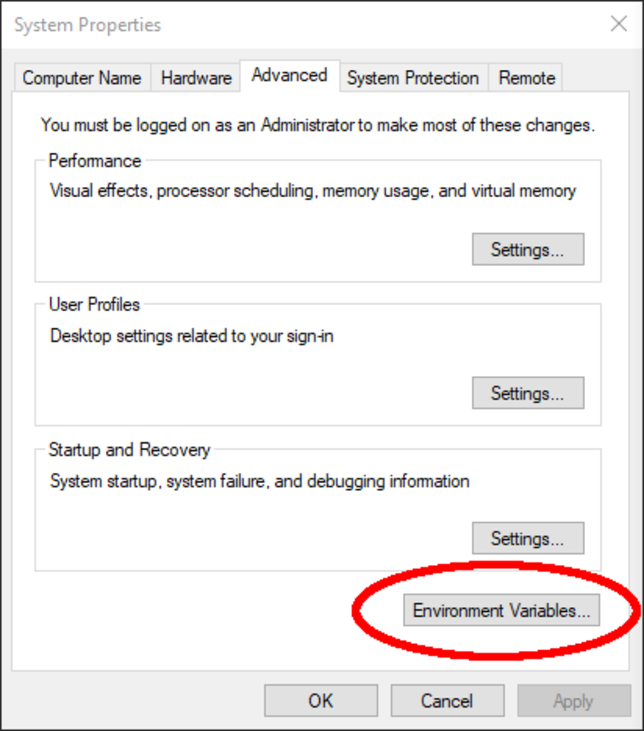
\includegraphics[width=\textwidth]{Figures/win/Win1.pdf}
(a)
\end{center}
\end{minipage}
\begin{minipage}[t]{.29\textwidth}
\begin{center}
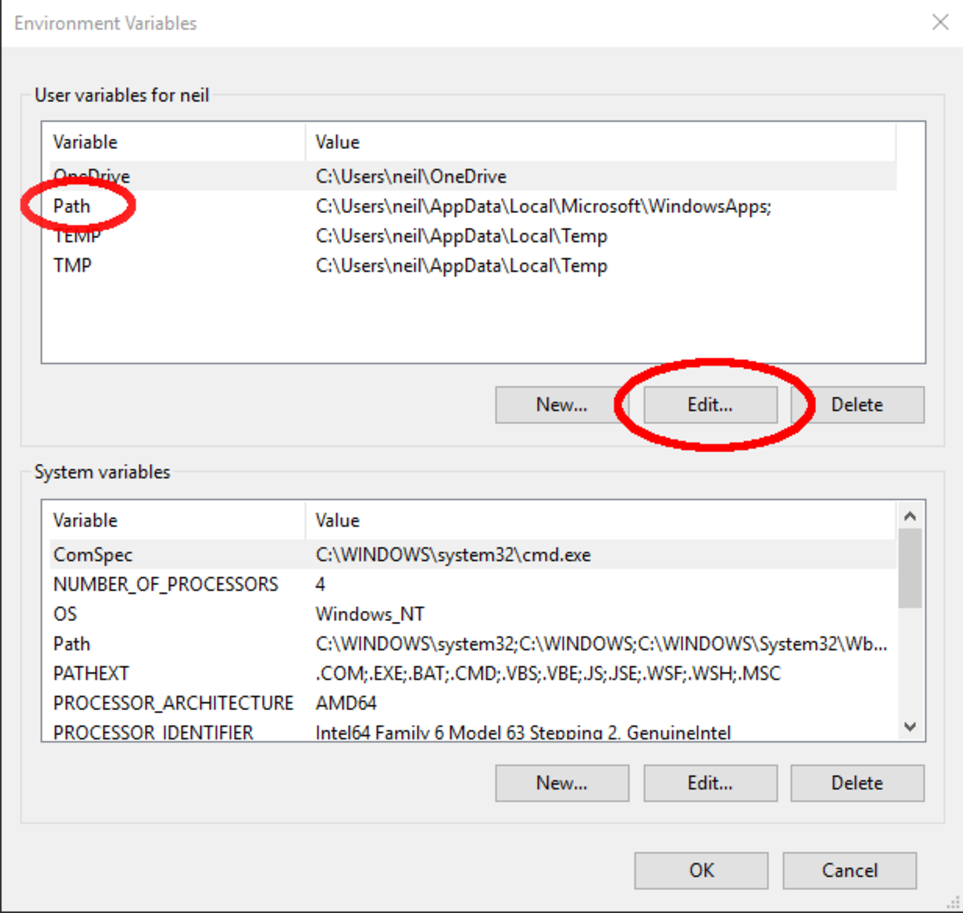
\includegraphics[width=\textwidth]{Figures/win/Win2.pdf}
(b)
\end{center}
\end{minipage}
\begin{minipage}[t]{.29\textwidth}
\begin{center}
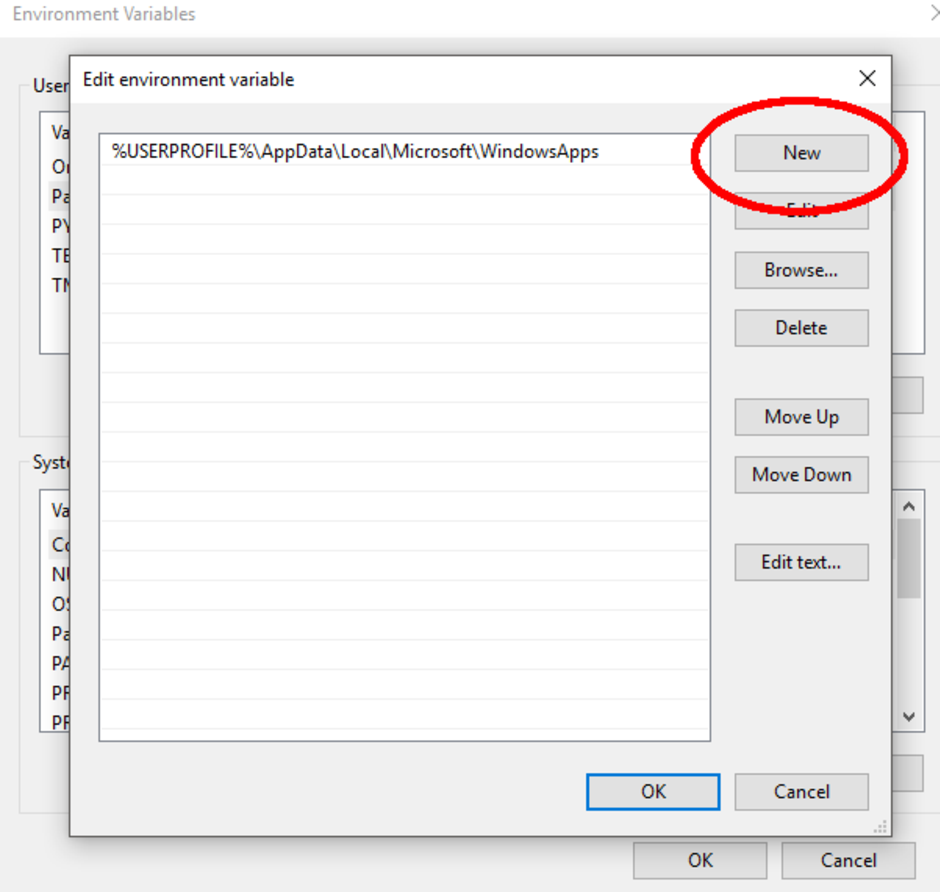
\includegraphics[width=\textwidth]{Figures/win/Win3.pdf}
(c)
\end{center}
\end{minipage}

\begin{minipage}[t]{.29\textwidth}
\begin{center}
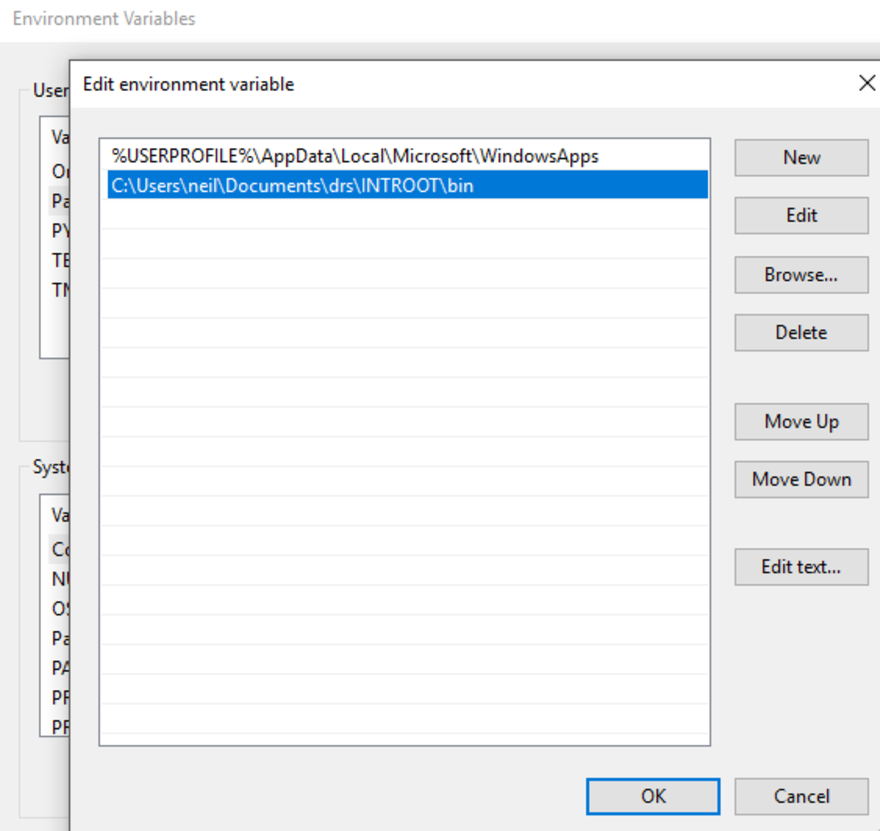
\includegraphics[width=\textwidth]{Figures/win/Win4.pdf}
(d)
\end{center}
\end{minipage}
\begin{minipage}[t]{.29\textwidth}
\begin{center}
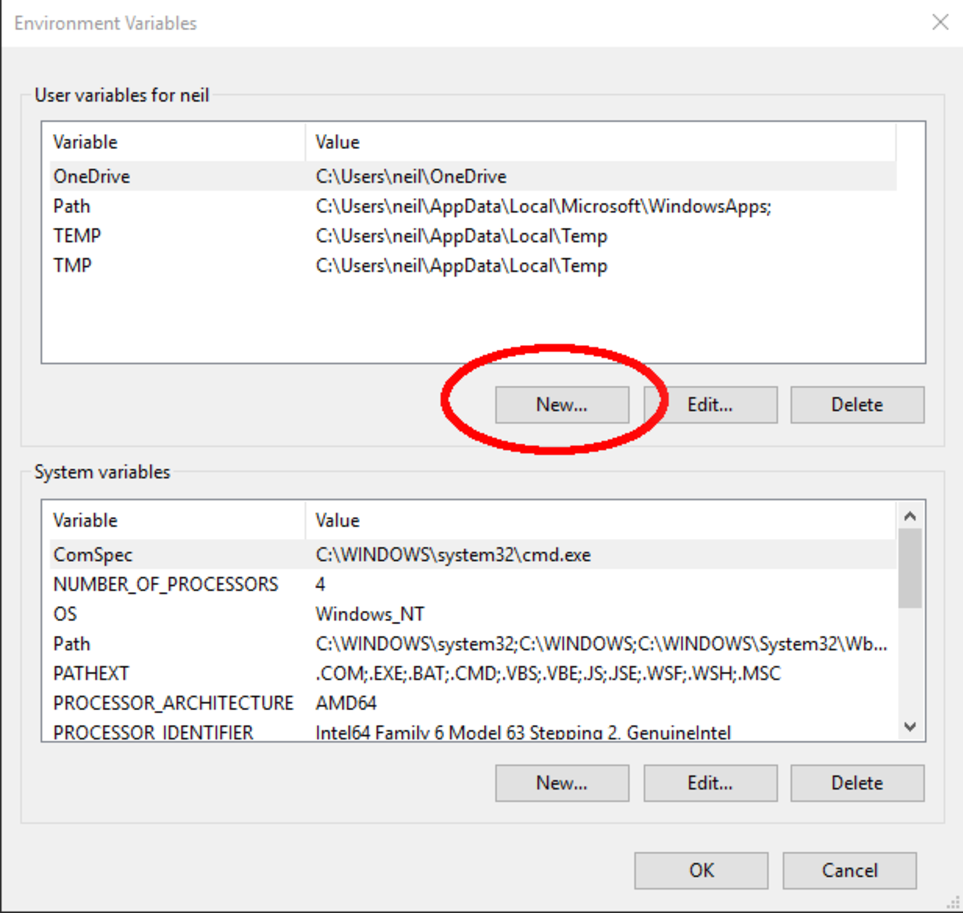
\includegraphics[width=\textwidth]{Figures/win/Win5.pdf}
(e)
\end{center}
\end{minipage}
\begin{minipage}[t]{.29\textwidth}
\begin{center}
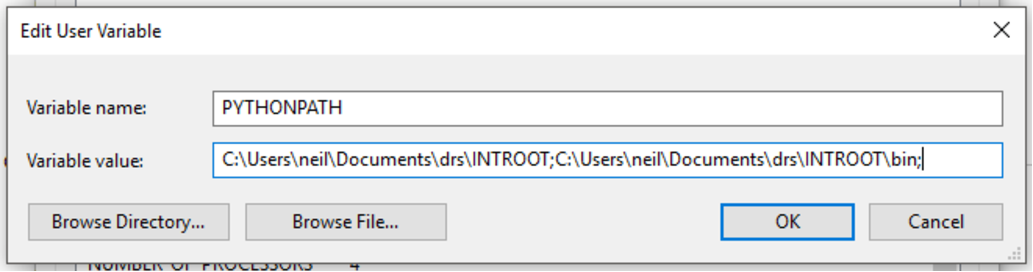
\includegraphics[width=\textwidth]{Figures/win/Win6.pdf}
(f)
\end{center}
\end{minipage}
\end{center}
\caption{(a) Once in ``Advanced system properties'' click ``Environment Variables'' (b) Click ``Path'' and click ``Edit...'' to edit the ``Path'' environmental variable (c) Once in the ``Path'' environmental variable click ``New'' to add a new path (d) Type in the new line to add variable and click ``OK'' (e) Once back in the Enivronmental variable page click ``New'' to add `PYTHONPATH' (f) Set the variable name to ``PYTHONPATH'' and edit the variable value accordingly. \label{figure:screengrabs} }
\end{figure}
\vspace{0.25cm}



%%%%%%%%%%%%%%%%%%%%%%%%%%%%%%%%%%%%%%%%%%%%%%%%%%%%%%%%
%%
\clearpage
\newpage
\section{Setting up the DRS (Windows)}
\label{ch:install:setup_win}
%%
%%%%%%%%%%%%%%%%%%%%%%%%%%%%%%%%%%%%%%%%%%%%%%%%%%%%%%%%

Before running the DRS one must set the data paths. \\

\noindent The `\configtxtfile' file is located in the \InstallDIR in the config folder.

i.e. at \InstallDIR\path{\\config\\}{configtxtfile} \\

\noindent The following keywords \textbf{must} be changed (and must be a valid path):
\begin{thighlight}
\begin{table}[H]
{\footnotesize
\begin{tabular}{p{4cm} p{0.05cm} p{2.5cm} p{0.05cm} p{5.5cm}}
\definevariable{text:drs_root}{TDATA}            & = & \path{C:\\Users\\User\\Documents\\drs\\data}        & / & Define the DATA directory\\
&&&&\\
\definevariable{text:drs_root}{DRS\_ROOT}         & = & \path{C:\\Users\\User\\Documents\\drs\\INTROOT}     & / & Define the installation directory \\
\definevariable{text:drs_data_raw}{DRS\_DATA\_RAW}     & = & \path{C:\\Users\\User\\Documents\\drs\\data\\raw}    & / & Define the folder with the raw data files in \\
\definevariable{text:drs_data_reduc}{DRS\_DATA\_REDUC}   & = & \path{C:\\Users\\User\\Documents\\drs\\data\\reduced} & / & Define the directory that the reduced data should be saved to/read from \\
\definevariable{text:drs_calib_db}{DRS\_CALIB\_DB}     & = & \path{C:\\Users\\User\\Documents\\drs\\data\\calibDB} & / & Define the directory that the calibration files should be saved to/read from \\
\definevariable{text:drs_data_msg}{DRS\_DATA\_MSG}     & = & \path{C:\\Users\\User\\Documents\\drs\\data\\msg}    & / & Define the directory that the log messages are stored in \\
\definevariable{text:drs_data_working}{DRS\_DATA\_WORKING} & = & \path{C:\\Users\\User\\Documents\\drs\\data\\tmp}    & / & Define the working directory \\
\end{tabular}
}
\end{table}
\end{thighlight}
\begin{note}
Note: On windows paths in windows must have a `\textbackslash\textbackslash' also the python files must be open with a valid editor such as sublime text, notepad++, spyder or pycharm for example
\end{note}

\vspace{0.25cm}

\noindent The following keywords can be changed: \\
\begin{thighlight}
\begin{table}[H]
\begin{tabular}{>{\color{red}}l c r c p{5cm}}
\definevariable{text:drs_plot}{DRS\_PLOT}    & = & 1     & / & Whether to show plots \\
\definevariable{text:print_level}{PRINT\_LEVEL} & = & "all" & / & Level at which to print \\
\definevariable{text:log_level}{LOG\_LEVEL}   & = & "all" & / & Level at which to log in log file \\
\end{tabular}
\end{table}

\noindent For the `\definevariable{text:print_level}{PRINT\_LEVEL} and \definevariable{text:log_level}{LOG\_LEVEL} keywords the values are set as follows:
\begin{itemize}
	\item "all" -- prints all events
	\item "info" -- prints info, warning and error events
	\item "warning" -- prints warning and error events
	\item "error" -- print only error events
\end{itemize}
\end{thighlight}



%%%%%%%%%%%%%%%%%%%%%%%%%%%%%%%%%%%%%%%%%%%%%%%%%%%%%%%%
%%
\clearpage
\newpage
\section{Validating Installation on Windows}
\label{ch:install:validating_installwin}
%%
%%%%%%%%%%%%%%%%%%%%%%%%%%%%%%%%%%%%%%%%%%%%%%%%%%%%%%%%

\begin{note}
One must install the DRS (Section \ref{ch:install:install_win}) AND set up the DRS (Section \ref{ch:install:setup}) before validation will be successful.
\end{note}

\noindent In windows there are currently 3 ways to run the RS (running in python/ipython).

\begin{itemize}
\item To validate running from python/ipython from the command line type:
\begin{cmdbox}
python (*\calvalidate*)
ipython (*\calvalidate*)
\end{cmdbox}

\item To validate running from ipython, open ipython and type:
\begin{pythonbox}
@run@ (*\calvalidate*)
\end{pythonbox}

\item To validate running from import from python/ipython, open python/ipython and type:
\begin{pythonbox}
import cal_validate_spirou
cal_validate_spirou.main()
\end{pythonbox}

\end{itemize}

\noindent If validation is successful the following should appear:
\begin{cmdboxprintspecial}
@g
17:34:19.0 -   || *****************************************
17:34:19.0 -   || * SPIROU @(#) Geneva Observatory (0.1.016)
17:34:19.0 -   || *****************************************
17:34:19.0 -   ||(dir_data_raw)      DRS_DATA_RAW=C:\\Users\\User\\Documents\\drs\\data\\raw
17:34:19.0 -   ||(dir_data_reduc)    DRS_DATA_REDUC=C:\\Users\\User\\Documents\\drs\\data\\reduced
17:34:19.0 -   ||(dir_calib_db)      DRS_CALIB_DB=C:\\Users\\User\\Documents\\drs\\data\\calibDB
17:34:19.0 -   ||(dir_data_msg)      DRS_DATA_MSG=C:\\Users\\User\\Documents\\drs\\data\\msg
17:34:19.0 -   ||(print_level)       PRINT_LEVEL=all         %(error/warning/info/all)
17:34:19.0 -   ||(log_level)         LOG_LEVEL=all         %(error/warning/info/all)
17:34:19.0 -   ||(plot_graph)        DRS_PLOT=1            %(def/undef/trigger)
17:34:19.0 -   ||(used_date)         DRS_USED_DATE=undefined
17:34:19.0 -   ||(working_dir)       DRS_DATA_WORKING=C:\\Users\\User\\Documents\\drs\\data\\tmp
17:34:19.0 -   ||                    DRS_INTERACTIVE is not set, running on-line mode
17:34:19.0 -   ||                    DRS_DEBUG is set, debug mode level:1
17:34:19.0 -   ||
17:34:19.0 -   ||Validation successful. DRS installed corrected.
@g
\end{cmdboxprintspecial}

% Chapter: Data Architecture
%%%%%%%%%%%%%%%%%%%%%%%%%%%%%%%%%%%%%%%%%%%%%%%%%%%%%%%%
%%
\chapter{Data Architecture}
\label{chapter:data_architecture}
%%
%%%%%%%%%%%%%%%%%%%%%%%%%%%%%%%%%%%%%%%%%%%%%%%%%%%%%%%%

% Chapter: Using the DRS
%%%%%%%%%%%%%%%%%%%%%%%%%%%%%%%%%%%%%%%%%%%%%%%%%%%%%%%%
%%
\chapter{Using the DRS}
\label{chapter:using_the_drs}
%%
%%%%%%%%%%%%%%%%%%%%%%%%%%%%%%%%%%%%%%%%%%%%%%%%%%%%%%%%

There are two ways to run the DRS recipes. The first (described in Section \ref{chapter:using_the_drs:direct}) directly calls the code and inputs arguments (either from the command line or from python), the second way is to import the recipes in a python script and define arguments in a call to a function (see Section \ref{chapter:using_the_drs:script}).

%%%%%%%%%%%%%%%%%%%%%%%%%%%%%%%%%%%%%%%%%%%%%%%%%%%%%%%%
%%
\section{Running the DRS recipes directly}
\label{chapter:using_the_drs:direct}
%%
%%%%%%%%%%%%%%%%%%%%%%%%%%%%%%%%%%%%%%%%%%%%%%%%%%%%%%%%

As in Chapter \ref{chapter:installation}, using Linux or \mac one can run DRS recipes from the command line or from python, in windows one is required to be in python before running the scipts. Below we use \calDARK as an example:
\begin{itemize}
\item To run from command line type:
\begin{cmdbox}
(*\calDARK*) YYMMDD Filenames
\end{cmdbox}

\item To run from python/ipython from the command line type:
\begin{cmdbox}
python (*\calDARK*) YYMMDD Filenames
ipython (*\calDARK*) YYMMDD Filenames
\end{cmdbox}

\item To run from ipython, open ipython and type:
\begin{pythonbox}
@run@ (*\calDARK*) YYMMDD Filenames
\end{pythonbox}
\end{itemize}

%%%%%%%%%%%%%%%%%%%%%%%%%%%%%%%%%%%%%%%%%%%%%%%%%%%%%%%%
%%
\section{Running the DRS recipes from a python script}
\label{chapter:using_the_drs:script}
%%
%%%%%%%%%%%%%%%%%%%%%%%%%%%%%%%%%%%%%%%%%%%%%%%%%%%%%%%%

In any operating system one can also import a recipe and call a function to run the code. This is useful in batch operations, timing tests and unit tests for example. Below we use \calDARK as an example:

\begin{pythonbox}
# import the recipe
import cal_DARK_spirou
# define the night folder name
night_name = "20170710"
# define the file(s) to run through the code
files = ['dark_dark02d406.fits']
# run code
cal_validate_spirou.main(night_name=night_name, files=files)
\end{pythonbox}


%%%%%%%%%%%%%%%%%%%%%%%%%%%%%%%%%%%%%%%%%%%%%%%%%%%%%%%%
%%
\section{Working example of the code for SPIRou}
\label{chapter:using_the_drs:working_example}
%%
%%%%%%%%%%%%%%%%%%%%%%%%%%%%%%%%%%%%%%%%%%%%%%%%%%%%%%%%

% ----------------------------------------------
\subsection{Overview}
\label{chapter:using_the_drs:working_example:overview}
% ----------------------------------------------

For this example all files are from:
\begin{cmdbox}
spirou@10.102.14.81:/data/RawImages/H2RG-AT4/AT4-04/2017-07-10_15-36-18/ramps/
\end{cmdbox} 

\noindent following our example data architecture (from Section \ref{ch:install:setup} and shown explicity in Section \ref{ch:data_architecture:folder_layout}) all files should be places in the \definevariable{text:drs_data_raw}{DRS\_DATA\_RAW} (\textcolor{blue}{/drs/data/raw} in our case).

\noindent and we will also need the current WAVE file from here:
\begin{cmdbox}
spirou@10.102.14.81:/data/reduced/DATA-CALIB/spirou_wave_ini3.fits
\end{cmdbox}

\noindent which needs to be placed in the \definevariable{text:drs_calib_db}{DRS\_CALIB\_DB} dirctory (\textcolor{blue}{/drs/data/calibDB} in our case).

\noindent Starting with RAMP files and ending with extracted orders and calculated drifts we need to run six codes:
\begin{enumerate}
\item \calDARK \hfill (See Section \ref{ch:the_recipes:cal_DARK_spirou})
\item \callocRAW ($\times$2) \hfill (See Section \ref{ch:the_recipes:cal_loc_RAW_spirou})
\item \calSLIT \hfill (See Section \ref{ch:the_recipes:cal_SLIT_spirou})
\item \calFFraw ($\times$2) \hfill (See Section \ref{ch:the_recipes:cal_FF_RAW_spirou})
\item (add spirou\_wave\_ini3.fits to calibDB) 
\item \calextractRAWAB and \calextractRAWC (many times) \hfill (See Section \ref{ch:the_recipes:cal_extract_RAW_spirou})
\item \calDRIFTRAW \hfill (See Section \ref{ch:the_recipes:cal_DRIFT_RAW_spirou})
\end{enumerate}





% ----------------------------------------------
\subsection{Run through from command line/python shell (Linux and macOS)}
\label{chapter:using_the_drs:working_example:run_cmd}
% ----------------------------------------------

As long as all codes are excutable (see Section \ref{ch:install:installunix:executable}) one can run all codes from the command line or if not excutable or one has a preference for python one can run the following with `python \{command\}', `ipython \{command\}' or indeed through an interactive ipython session using `run \{command\}'.

\begin{enumerate}

\item run the dark extraction on the `dark\_dark' file:
\begin{cmdbox}
cal_DARK_spirou.py 20170710 dark_dark02d406.fits
\end{cmdbox}

\item run the order localisation on the `dark\_flat' files:
\begin{cmdbox}
cal_loc_RAW_spirou.py 20170710 dark_flat02f10.fits dark_flat03f10.fits dark_flat04f10.fits dark_flat05f10.fits dark_flat06f10.fits
\end{cmdbox}

\item run the order localisation on the `flat\_dark' files:
\begin{cmdbox}
cal_loc_RAW_spirou.py 20170710 flat_dark02f10.fits flat_dark03f10.fits flat_dark04f10.fits flat_dark05f10.fits flat_dark06f10.fits
\end{cmdbox}

\item run the slit calibration on the `fp\_fp' files.
\begin{cmdbox}
cal_SLIT_spirou.py 20170710 fp_fp02a203.fits fp_fp03a203.fits fp_fp04a203.fits
\end{cmdbox}

\item run the flat field creation on the `dark\_flat' files:

\begin{note}
if using same files as above you will get an error message when running the file.

\noindent To solve this open the `\masterCALIBDBfile' file located in \textcolor{blue}{\{DATA\_ROOT\_CALIB\}}. Edit the unix date in the line that begins `TILT' so that it is less than or equal to the unix date on rows `ORDER\_PROFIL\_AB' (i.e. easiest to change it to the date on the `ORDER\_PROFIL\_AB')

\noindent The human date format must match the unix date thus both must be changed if one is modified.

\noindent i.e. the `\masterCALIBDBfile' file should look go from
\begin{textbox}
DARK 20170710 dark_dark02d406.fits 07/10/17/16:37:48 1499704668.0
ORDER_PROFIL_C 20170710 dark_flat02f10_order_profil_C.fits 07/10/17/17:03:50 1499706230.0
LOC_C 20170710 dark_flat02f10_loco_C.fits 07/10/17/17:03:50 1499706230.0
ORDER_PROFIL_AB 20170710 flat_dark02f10_order_profil_AB.fits 07/10/17/17:07:08 1499706428.0
LOC_AB 20170710 flat_dark02f10_loco_AB.fits 07/10/17/17:07:08 1499706428.0
TILT 20170710 fp_fp02a203_tilt.fits @07/10/17/17:25:15 1499707515.0@
\end{textbox}
\noindent to this:
\begin{textbox}
DARK 20170710 dark_dark02d406.fits 07/10/17/16:37:48 1499704668.0
ORDER_PROFIL_C 20170710 dark_flat02f10_order_profil_C.fits 07/10/17/17:03:50 1499706230.0
LOC_C 20170710 dark_flat02f10_loco_C.fits 07/10/17/17:03:50 1499706230.0
ORDER_PROFIL_AB 20170710 flat_dark02f10_order_profil_AB.fits 07/10/17/17:07:08 1499706428.0
LOC_AB 20170710 flat_dark02f10_loco_AB.fits 07/10/17/17:07:08 1499706428.0
TILT 20170710 fp_fp02a203_tilt.fits @07/10/17/17:07:08 1499706428.0@
\end{textbox}
\end{note}

\begin{cmdbox}
cal_FF_RAW_spirou.py 20170710 dark_flat02f10.fits dark_flat03f10.fits dark_flat04f10.fits dark_flat05f10.fits dark_flat06f10.fits
\end{cmdbox}

\newpage

\item Currently we do not create a new wavelength calibration file for this run. Therefore we need one (as stated in the above section). We use the one from here:
\begin{cmdbox}
spirou@10.102.14.81:/data/reduced/DATA-CALIB/spirou_wave_ini3.fits
\end{cmdbox}

\noindent then place it in the \definevariable{text:drs_calib_db}{DRS\_CALIB\_DB} folder. You will also need to edit the `\masterCALIBDBfile' file located in \definevariable{text:drs_calib_db}{DRS\_CALIB\_DB}. 

\noindent Add the folloing line to `\masterCALIBDBfile'
\begin{textbox}
@WAVE 20170710 spirou_wave_ini3.fits 07/10/17/17:03:50 1499706230.0@
\end{textbox}

\noindent and the `master\_calib\_SPIROU.txt' should look like this:
\begin{textbox}
DARK 20170710 dark_dark02d406.fits 07/10/17/16:37:48 1499704668.0
ORDER_PROFIL_C 20170710 dark_flat02f10_order_profil_C.fits 07/10/17/17:03:50 1499706230.0
LOC_C 20170710 dark_flat02f10_loco_C.fits 07/10/17/17:03:50 1499706230.0
ORDER_PROFIL_AB 20170710 flat_dark02f10_order_profil_AB.fits 07/10/17/17:07:08 1499706428.0
LOC_AB 20170710 flat_dark02f10_loco_AB.fits 07/10/17/17:07:08 1499706428.0
TILT 20170710 fp_fp02a203_tilt.fits 07/10/17/17:07:08 1499706428.0
@WAVE 20170710 spirou_wave_ini3.fits 07/10/17/17:03:50 1499706230.0@
\end{textbox}

\item run the extraction files on the `hcone\_dark', `dark\_hcone', `hcone\_hcone', `dark\_dark\_AHC1', `hctwo\_dark', `dark\_hctwo', `hctwo-hctwo', `dark\_dark\_AHC2' and `fp\_fp'  files. For example for the `fp\_fp' files:
\begin{cmdbox}
cal_extract_RAW_spirouAB.py 20170710 fp_fp02a203.fits fp_fp03a203.fits fp_fp04a203.fits
cal_extract_RAW_spirouC.py 20170710 fp_fp02a203.fits fp_fp03a203.fits fp_fp04a203.fits
\end{cmdbox}

\item run the drift calculation on the `fp\_fp' files:
\begin{cmdbox}
@cal_DRIFT_RAW_spirou.py 20170710 @fp_fp02a203.fits fp_fp03a203.fits fp_fp04a203.fits
\end{cmdbox}

\end{enumerate}

% ----------------------------------------------
\clearpage
\newpage
\subsection{Run through python script}
\label{chapter:using_the_drs:working_example:run_python}
% ----------------------------------------------

The process is in the same order as Section \ref{chapter:using_the_drs:working_example:run_cmd}, including changing the date on the `TILT' keyword and adding the `WAVE' line, and adding the wave file to the calibDB folder).

\begin{pythonbox}
import cal_DARK_spirou, cal_loc_RAW_spirou
import cal_SLIT_spirou, cal_FF_RAW_spirou
import cal_extract_RAW_spirou, cal_DRIFT_RAW_spirou
import matplotlib.pyplot as plt
# define constants
NIGHT_NAME = '20170710'
# cal_dark_spirou
files = ['dark_dark02d406.fits']          # set up files
cal_DARK_spirou.main(NIGHT_NAME, files)   # run cal_dark_spirou
plt.close('all')                          # close graphs
# cal_loc_RAW_spirou - flat_dark
files = ['flat_dark02f10.fits', 'flat_dark03f10.fits', 'flat_dark04f10.fits',
         'flat_dark05f10.fits','flat_dark06f10.fits']
cal_loc_RAW_spirou.main(NIGHT_NAME, files)
plt.close('all')
# cal_loc_RAW_spirou - dark_flat
files = ['dark_flat02f10.fits', 'dark_flat03f10.fits', 'dark_flat04f10.fits', 
         'dark_flat05f10.fits', 'dark_flat06f10.fits']
cal_loc_RAW_spirou.main(NIGHT_NAME, files)
plt.close('all')
# cal_SLIT_spirou
files = ['fp_fp02a203.fits', 'fp_fp03a203.fits', 'fp_fp04a203.fits']
cal_SLIT_spirou.main(NIGHT_NAME, files)
plt.close('all')
# cal_FF_RAW_spirou - flat_dark
files = ['flat_dark02f10.fits', 'flat_dark03f10.fits','flat_dark04f10.fits',
         'flat_dark05f10.fits', 'flat_dark06f10.fits']
cal_FF_RAW_spirou.main(NIGHT_NAME, files)
plt.close('all')
# cal_FF_RAW_spirou - dark_flat
files = ['dark_flat02f10.fits', 'dark_flat03f10.fits', 'dark_flat04f10.fits', 
         'dark_flat05f10.fits', 'dark_flat06f10.fits']
cal_FF_RAW_spirou.main(NIGHT_NAME, files)
plt.close('all')
# cal_extract_RAW_spirou - fp_fp AB
files = ['fp_fp02a203.fits', 'fp_fp03a203.fits', 'fp_fp04a203.fits']
cal_extract_RAW_spirou.main(NIGHT_NAME, files, 'AB')
plt.close('all')
# cal_extract_RAW_spirou - fp_fp C
files = ['fp_fp02a203.fits', 'fp_fp03a203.fits', 'fp_fp04a203.fits']
cal_extract_RAW_spirou.main(NIGHT_NAME, files, 'C')
plt.close('all')
# test cal_DRIFT_RAW_spirou
files = ['fp_fp02a203.fits', 'fp_fp03a203.fits', 'fp_fp04a203.fits']
cal_DRIFT_RAW_spirou.main(NIGHT_NAME, files)
plt.close('all')

\end{pythonbox}


% Chapter: Changelog (This version and AT-4)
%%%%%%%%%%%%%%%%%%%%%%%%%%%%%%%%%%%%%%%%%%%%%%%%%%%%%%%%
%%
\chapter{Summary of changes (AT-4)}
\label{ch:changelog}
%%
%%%%%%%%%%%%%%%%%%%%%%%%%%%%%%%%%%%%%%%%%%%%%%%%%%%%%%%%

Below we describe breifly the main differences from AT-4 build.

%%%%%%%%%%%%%%%%%%%%%%%%%%%%%%%%%%%%%%%%%%%%%%%%%%%%%%%%
%%
\section{General}
%%
%%%%%%%%%%%%%%%%%%%%%%%%%%%%%%%%%%%%%%%%%%%%%%%%%%%%%%%%
\begin{itemize}

\item all recipes main body of code is now in a \definevariable{\progMAIN} function and this function is called in \definevariable{\MAIN} part of the code (the part that executes at run time). This allows recipes to be called as functions as well as being called as a standalone code or from the command line. i.e. for \calDARK:
	\begin{pythonbox}
	import cal_DARK_spirou
	    
	files = ['dark_dark02d406.fits']
	night_name = '20170710'
	cal_DARK_spirou.main(night_name=night_name, files=files)
	\end{pythonbox}
	will run the exact same procedure as:
	\begin{bashbox}
	cal_DARK_spirou.py 201707 dark_dark02d406.fits
	\end{bashbox}

\item \definevariable{WLOG} function overhal (now in \definevariable{\spirouLog.logger()}) but aliased in most codes back to \definevariable{WLOG}. This means one can use the same functionality as before:
	\begin{pythonbox}
	WLOG("warning", "program", "message")
	\end{pythonbox}
	However now when "error" is called an automatic exit routine is run (therefore there is no need for sys.exit after a WLOG("error", "", "") call).

\item execution of pythonstartup codes removed and replaced with functions

\item loading of many variables into python memory replaced with call to need dictionary object (parameter dictionary). Parameter dictionary is a custom dictionary object that as well as storing key and value pairs also can set a source for each key in the dictionary (hence the developer will always know where a variable was defined, if used correctly)

\item All hard coded constants removed from running code and moved to configuration files, all variables have been described, noted their new definition locations and where they are used in the recipes and codes (see Section \ref{ch:variables}). This has allowed (and will allow) variables to either be public (i.e. in a location easily accessible by the user) or to be private (in files stored within the module). We can make many specific configuration files or a few, depending on which we deem best.

\item Custom exception: \definevariable{ConfigError} and \definevariable{ConfigException} - designed specifically to be used with the WLOG() function 

\item moved core functions used in multiple recipes to sub-modules

\item all plotting taken out of main codes (call to specific sub-module)

\end{itemize}

%%%%%%%%%%%%%%%%%%%%%%%%%%%%%%%%%%%%%%%%%%%%%%%%%%%%%%%%
%%
\section{The cal\_DARK\_spirou recipe}
\label{ch:changelog:At4:cal_DARK_spirou}
%%
%%%%%%%%%%%%%%%%%%%%%%%%%%%%%%%%%%%%%%%%%%%%%%%%%%%%%%%%

\begin{itemize}

\item dark measurement moved to function \definevariable{\spirouImage.MeasureDark} (for clarity). This is, in part, due to the repetition of code for ``Whole det'', ``Blue part'' and ``Red part''.

\item all plotting moved to internal functions (for clarity)
	\begin{itemize}
    \item \definevariable{\spirouPlot.darkplot\_image\_and\_regions} for the image/region plot
    \item \definevariable{\spirouPlot.darkplot\_datacut} for the DARK cutlimit plot
    \item \definevariable{\spirouPlot.darkplot\_histograms} for the histogram plots 
    \end{itemize}

\item histogram plot updated, original plot plotted bin centers as a smooth peak, simple modification to make sure histogram bars are present
    
\item writing of data is sped up by caching all HEADER keys and writing to file once with the write of the data.

\item speed up
	\begin{itemize}
	\item AT-4 v44: 4.881 seconds
	\item py3: 1.890 seconds
	\end{itemize}

\end{itemize}

%%%%%%%%%%%%%%%%%%%%%%%%%%%%%%%%%%%%%%%%%%%%%%%%%%%%%%%%
%%
\section{The cal\_loc\_RAW\_spirou recipe}
\label{ch:changelog:At4:cal_loc_RAW_spirou}
%%
%%%%%%%%%%%%%%%%%%%%%%%%%%%%%%%%%%%%%%%%%%%%%%%%%%%%%%%%

\begin{itemize}

\item added function to convert from ADU/s to electrons \definevariable{\spirouImage.ConvertToE}
    
\item added function to flip image \definevariable{\spirouImage.FlipImage}

\item smoothed image (by a box) is now in a function (creates order\_profile)
	\begin{itemize}
	\item added different way to calculate order\_profile - currently set to 'manual' be default
	\item \definevariable{\spirouLOCOR.BoxSmoothedImage} 
	\item Instead of manually working out the mean for each box you convolve the weighted image with a tophat function and the weights with a topcat function and then divide the two.
	\item This gives approximately the same result (with small deviations due to the FT of a topcat function not being perfect).
	\item The function can be turned back to the original manual mode by using `mode='manual'' but is slower (by a factor of $\sim\times$8)
	\end{itemize}

\item added storage dictionary to store (and pass around) all variables created `loc' - a Parameter dictionary (thus source can be set for all variables to keep track of them)

\item added function to measure background and get central pixel positions \definevariable{\spirouLOCOR.MeasureBkgrdGetCentPixs}

\item debug plot added to plot the minimum of `ycc' and `ic\_locseuil' \definevariable{\spirouPlot.sPlt.debug\_locplot\_min\_ycc\_loc\_threshold}

\item added function for locating central position (previously \definevariable{\spirouLOCOR.poscolc}) - currently set to 'manual' be default
    \begin{itemize}
    \item \definevariable{\spirouLOCOR.LocateCentralOrderPositions} 
    \item  Instead of manually working out the starts and ends of each order (with while loops) convolves a mask of cvalues > threshold with a top-hat (size=3) function such that all edges are found
    \item i.e. `[False, True, True]` or `[True, True, False]` give a different value than `[True, True, True]` or `[False, False, False]` or `[False, False, True]`
    \item i.e. the convolution gives the sum of three elements, thus selected those elements with a sum of 2 give our edges
    \item The function can be turned back to the original 'manual' mode by using `mode='manual` but is slower (by a factor of x2)
	\end{itemize}

\item debug plot added to plot the image above saturation threshold \definevariable{\spirouPlot.locplot\_im\_sat\_threshold}
        
\item moved `ctro`,`sigo`,`ac`,`ass` etc into loc (for storage and ease of use)        
        
\item the fit across each order has been split into functions
    \begin{itemize}
	\item the initial fit is done by \definevariable{\spirouLOCOR.InitialOrderFit}
	\item This initial fit takes in the plotting args and thus as order is fit the fit is piped on to plot via \definevariable{\spirouPlot.locplot\_order}
	\item the sigma clipping fit is done by \definevariable{\spirouLOCOR.SigClipOrderFit}
	\item kind is used to change between 'center' and 'fwhm' fits (thus function is reused in both cases), kind will do the tiny bits of code which are different for each fit
	\item all fit parameters are loaded into the `loc` parameter dictionary
	\end{itemize}

\item plot of order number against rms is move to \definevariable{\spirouPlot.locplot\_order{\hskip 0pt}\_number\_against\_rms}

\item function created to add the 2Dlist (i.e. the coefficients) to hdict (the dictionary used to save keys to so that we only write to the fits file once)

\item superimposed fit on the image is pushed into a function, this is many times faster than before - due to optimisation, \definevariable{\spirouLOCOR.imageLocSuperimp}

\item Writing of fits file cleaned up (header keywords written during data write)

\item speed up
	\begin{itemize}
	\item AT-4 v44: 5.697 seconds
	\item py3:  2.255 seconds
    \end{itemize}

\end{itemize}

%%%%%%%%%%%%%%%%%%%%%%%%%%%%%%%%%%%%%%%%%%%%%%%%%%%%%%%%
%%
\section{The cal\_SLIT\_spirou recipe}
\label{ch:changelog:At4:cal_SLIT_spirou}
%%
%%%%%%%%%%%%%%%%%%%%%%%%%%%%%%%%%%%%%%%%%%%%%%%%%%%%%%%%

\begin{itemize}
\item added storage dictionary to store (and pass around) all variables created `loc` - a Parameter dictionary (thus source can be set for all variables to keep track of them)

\item Retrieval of coefficients from `\_loco\_` file moved to \definevariable{\spirouLOCOR.GetCoeffs}

\item Tilt finding is moved to function \definevariable{\spirouImage.GetTilt}

\item Fitting the tilt is moved to function \definevariable{\spirouImage.FitTilt}

\item selected order plot moved to \definevariable{\spirouPlot.slit\_sorder\_plot}

\item slit tilt angle and fit plot moved to \definevariable{\spirouPlot.slit\_tilt\_angle\_and\_fit\_plot}

\item Writing of fits file cleaned up (header keywords written during data write)

\item speed up
	\begin{itemize}
	\item AT-4 v44: 11.071 seconds
	\item py3: 4.386 seconds
    \end{itemize}

\end{itemize}

%%%%%%%%%%%%%%%%%%%%%%%%%%%%%%%%%%%%%%%%%%%%%%%%%%%%%%%%
%%
\section{The cal\_FF\_RAW\_spirou recipe}
\label{ch:changelog:At4:cal_FF_RAW_spirou}
%%
%%%%%%%%%%%%%%%%%%%%%%%%%%%%%%%%%%%%%%%%%%%%%%%%%%%%%%%%

\begin{itemize}
\item added function to replace measure\_bkgr\_FF, but incomplete (not currently used) would need to convert interpol.c to python (spline fitting)

\item added storage dictionary to store (and pass around) all variables created `loc` - a Parameter dictionary (thus source can be set for all variables to keep track of them)

\item Created function to read TILT file from calibDB (replaces `readkeyloco`)
	\begin{itemize}
    \item \definevariable{\spirouImage.ReadTiltFile}
    \item takes in header dictionary from `fitsfilename` in order to avoid re-opening FITS rec (acqutime used in calibDB to get max\_time of calibDB entry) 
    \end{itemize}
\item Created function to read order profile (replaces `read\_data\_raw` + pre-amble)
	\begin{itemize}
	\item \definevariable{\spirouImage.ReadOrderProfile}
	\item takes in header dictionary from `fitsfilename` in order to avoid re-opening FITS rec (acqutime used in calibDB to get max\_time of calibDB entry) 
    \end{itemize}
\item Used \definevariable{\spirouLOCOR.GetCoeffs} to get the coefficients from file

\item Created merge coefficients function to perform AB coefficient merge \definevariable{\spirouLOCOR.MergeCoefficients}
    
\item Updated extraction function \definevariable{\spirouEXTOR.ExtracTiltWeightOrder2} - much faster as takes many of the calculations outside the pixel loop
	\begin{itemize}
	\item i.e. calculating the pixel contribution due to tilt in array `ww`
	\item `ww` is constant for an order, thus doesn't need to be worked out for each pixel in one order, just the multiplication between ww and the image
	\item up to 8 times faster with these improvements
    \end{itemize}
\item `e2ds`, `SNR`, `RMS`, `blaze` and `flat` are stored in `loc` parameter dictionary

\item Plotting code moved to \definevariable{\spirouPlot} functions

\item Writing of fits file cleaned up (header keywords written during data write)

\item QC (max\_signal $>$ qc\_max\_signal $\times$ nbframes) moved to end, however in old code it is not used as a failure criteria so also not used to fail in new code

\item speed up
	\begin{itemize}
	\item AT-4 v44: 25.962 seconds
	\item py3: 4.675 seconds
    \end{itemize}

\end{itemize}

%%%%%%%%%%%%%%%%%%%%%%%%%%%%%%%%%%%%%%%%%%%%%%%%%%%%%%%%
%%
\section{The cal\_extract\_RAW\_spirou recipes}
\label{ch:changelog:At4:cal_extract_RAW_spirou}
%%
%%%%%%%%%%%%%%%%%%%%%%%%%%%%%%%%%%%%%%%%%%%%%%%%%%%%%%%%

\begin{itemize}
\item Merged \definevariable{cal\_extract{\hskip 0pt}\_RAW\_spirouAB}, \definevariable{cal\_extract{\hskip 0pt}\_RAW\_spirouC} and \definevariable{cal\_extract\_RAW{\hskip 0pt}\_spirouALL} can still access \definevariable{cal\_extract{\hskip 0pt}\_RAW\_spirouAB} and \definevariable{cal\_extract{\hskip 0pt}\_RAW\_spirouC} but instead of being modified copies of the code they are just wrappers for \definevariable{cal\_extract\_RAW{\hskip 0pt}\_spirou.py} (i.e. they forward the fiber type)

\item added storage dictionary to store (and pass around) all variables created `loc` - a Parameter dictionary (thus source can be set for all variables to keep track of them)

\item Created function to read TILT file from calibDB (replaces `readkeyloco`)
    \begin{itemize}
	\item \definevariable{\spirouImage.ReadTiltFile}
	\item takes in header dictionary from `fitsfilename` in order to avoid re-opening FITS rec (acqutime used in calibDB to get max\_time of calibDB entry) 
    \end{itemize}

\item Created function to read WAVE file from calibDB (replaces `read\_data\_raw(`)
    \begin{itemize}
	\item \definevariable{\spirouImage.ReadWaveFile}
	\item takes in header dictionary from `fitsfilename` in order to avoid re-opening FITS rec (acqutime used in calibDB to get max\_time of calibDB entry) 
    \end{itemize}

\item Used \definevariable{\spirouLOCOR.GetCoeffs} to get the coefficients from file

\item Created function to read order profile (replaces `read\_data\_raw` + pre-amble)
    \begin{itemize}
	\item \definevariable{\spirouImage.ReadOrderProfile}
	\item takes in header dictionary from `fitsfilename` in order to avoid re-opening FITS rec (acqutime used in calibDB to get max\_time of calibDB entry) 
    \end{itemize}

\item Created merge coefficients function to perform AB coefficient merge \definevariable{\spirouLOCOR.MergeCoefficients}

\item New structures above replace the need for specific fiber sections ('AB', 'C', 'A', 'B') (In \definevariable{cal\_extract{\hskip 0pt}\_RAW\_spirouALL} and individual setups for \definevariable{cal\_extract{\hskip 0pt}\_RAW\_spirouAB} and \definevariable{cal\_extract{\hskip 0pt}\_RAW\_spirouC})

\item all extraction functions passed into \definevariable{spirouEXTOR} to wrapper functions (\definevariable{\spirouEXTOR.ExtractOrder}, \definevariable{\spirouEXTOR.ExtractTiltOrder}, \definevariable{\spirouEXTOR.ExtractTiltWeightOrder} and \definevariable{\spirouEXTOR.ExtractWeightOrder}) these are then run into \definevariable{\spirouEXTOR.ExtractionWrapper} and processed accordingly

\item Added a timing string (to record timings of all extraction processes) use `print(timing))` to view
    
\item `e2ds` and `SNR` stored in `loc`

\item Plotting code moved to \definevariable{\spirouPlot} functions

\item Writing of fits file cleaned up (header keywords written during data write)

\item QC (max\_signal $>$ qc\_max\_signal $\times$ nbframes) moved to end, however in old code it is not used as a failure criteria so also not used to fail in new code

\item speed up
	\begin{itemize}
	\item AT-4 v44: 60.852
	\item py3: 8.694

	\item Extraction timing Py3:
		\begin{itemize}
		\item ExtractOrder = 0.025 s
		\item ExtractTiltOrder = 0.060 s
		\item ExtractTiltWeightOrder = 0.141 s
		\item ExtractWeightOrder = 0.070 s
         \end{itemize}

	\item Extraction timing AT-4 v46:
		\begin{itemize}
		\item ExtractOrder (Fortran) = 0.019 s
		\item ExtractOrder (Py2) = 0.085 s
		\item ExtractTiltOrder = 0.766 s
		\item ExtractTiltWeightOrder = 0.840 s
		\item ExtractWeightOrder = 0.156 s
         \end{itemize}

	\item Speed increase (Py3 over AT-4 v46)
		\begin{itemize}
		\item ExtractOrder (Py3 $\rightarrow$ Fortran) = slower    x 1.3 times slower
		\item ExtractOrder (Py3 $\rightarrow$ Py) = faster     x 3.4 times faster
		\item ExtractTiltOrder (Py3 $\rightarrow$ Py = faster     x12.9 times faster
		\item ExtractTiltWeightOrder (Py3 $\rightarrow$ Py) = faster    x6.0 times faster
		\item ExtractWeightOrder (Py3 $\rightarrow$ Py) = faster    x2.2 times faster
		\end{itemize}

	\end{itemize}

\end{itemize}


%%%%%%%%%%%%%%%%%%%%%%%%%%%%%%%%%%%%%%%%%%%%%%%%%%%%%%%%
%%
\section{The cal\_DRIFT\_RAW\_spirou recipe}
\label{ch:changelog:At4:cal_DRIFT_RAW_spirou}
%%
%%%%%%%%%%%%%%%%%%%%%%%%%%%%%%%%%%%%%%%%%%%%%%%%%%%%%%%%

\begin{itemize}
\item acqtime (bjdref) got from header using \definevariable{\spirouImage.GetAcqTime}
	\begin{itemize}
	\item can be used to get both `human` readible and `unix` time (use key kind=`human` or kind=`unix)
	\end{itemize}

\item Created function to read TILT file from calibDB (replaces `readkeyloco`)
	\begin{itemize}
	\item \definevariable{\spirouImage.ReadTiltFile}
	\item takes in header dictionary from `fitsfilename` in order to avoid re-opening FITS rec (acqutime used in calibDB to get max\_time of calibDB entry) 
	\end{itemize}

\item Created function to read WAVE file from calibDB (replaces `read\_data\_raw(`)
	\begin{itemize}
	\item \definevariable{\spirouImage.ReadWaveFile}
	\item takes in header dictionary from `fitsfilename` in order to avoid re-opening FITS rec (acqutime used in calibDB to get max\_time of calibDB entry) 
	\end{itemize}

\item Used \definevariable{\spirouLOCOR.GetCoeffs} to get the coefficients from file

\item Created function to read order profile (replaces `read\_data\_raw` + pre-amble)
	\begin{itemize}
	\item \definevariable{\spirouImage.ReadOrderProfile}
	\item takes in header dictionary from `fitsfilename` in order to avoid re-opening FITS rec (acqutime used in calibDB to get max\_time of calibDB entry) 
	\end{itemize}

\item new extraction (see \calextractRAW above).

\item delta RV RMS calculation in \definevariable{\spirouRV.DeltaVrms2D}
	\begin{itemize}
	\item where arguments are `speref` and `wave` (stored in `loc`)
	\item where keyword arguments are `sigdet`, `size` and `threshold` (stored in p)
	\end{itemize}

\item all functionality to do with listing files moved to \definevariable{\spirouImage{\hskip 0pt}.GetAllSimilarFiles} - no need for "alphanumeric short"/"nice sort" - `np.sort(x)` does this
    
\item Renormlisation and cosmics correction in \definevariable{\spirouRV.ReNormCosmic2D}
	\begin{itemize}
	\item where arguments are `speref` and `spe` (stored in `loc`)
	\item where keyword arguments are `cut`, `size` and `threshold` (stored in p)
	\end{itemize}

\item RV drift calculated
	\begin{itemize}
	\item \definevariable{\spirouRV.CalcRVdrift2D}
	\item where arguments are `speref`, `spen` and `wave` (`speref` and `spen` stored in loc)
	\item where keyword arguments are `sigdet`, `size` and `threshold` (stored in p)
	\end{itemize}

\item added an option (drift\_type\_e2ds) to decide between getting drift using a weighted mean or using a median (to combine all orders)

\item `drift`, `errdrift`, `deltatime`, `mdrift`, `merrdrift` stored in loc

\item Writing of fits file cleaned up (header keywords written during data write)

\item speed up
	\begin{itemize}
	\item AT-4 v44: 22.556 s
	\item py3:  8.143 s
	\end{itemize}

\end{itemize}


%%%%%%%%%%%%%%%%%%%%%%%%%%%%%%%%%%%%%%%%%%%%%%%%%%%%%%%%
%%
\section{The cal\_BADPIX\_spirou recipe}
\label{ch:changelog:At4:cal_BADPIX_spirou}
%%
%%%%%%%%%%%%%%%%%%%%%%%%%%%%%%%%%%%%%%%%%%%%%%%%%%%%%%%%

\begin{itemize}
	\item loading of custom arguments moved to \definevariable{\spirouStartup.GetCustomFromRuntime}

	\item loading of files moved to \definevariable{\spirouImage.ReadImage}

	\item normalising flat and median of flat moved to \definevariable{\spirouImage.NormMedianFlat}

	\item locating bad pixels moved to \definevariable{\spirouImage.LocateBadPixels}

	\item instead of taking the 90th pixel in flattened meadian flat image now work out the 90th percentile of finite values (will lead to a slightly more correct normalisation value)

	\item Writing of fits file cleaned up (header keywords written during data write)
\end{itemize}


%%%%%%%%%%%%%%%%%%%%%%%%%%%%%%%%%%%%%%%%%%%%%%%%%%%%%%%%
%%
\section{The cal\_DRIFT\_RAW\_spirou recipe}
\label{ch:changelog:At4:cal_DRIFT_RAW_spirou}
%%
%%%%%%%%%%%%%%%%%%%%%%%%%%%%%%%%%%%%%%%%%%%%%%%%%%%%%%%%

\begin{itemize}
\item loading of custom arguments for reference file

\item acqtime (bjdref) got from header using \definevariable{\spirouImage.GetAcqTime}
	\begin{itemize}
	\item can be used to get both `human` readible and `unix` time (use key kind=`human` or kind=`unix)
	\end{itemize}

\item Created function to read TILT file from calibDB (replaces `readkeyloco`)
	\begin{itemize}
	\item \definevariable{\spirouImage.ReadTiltFile}
	\item takes in header dictionary from `fitsfilename` in order to avoid re-opening FITS rec (acqutime used in calibDB to get max\_time of calibDB entry) 
	\end{itemize}

\item Created function to read WAVE file from calibDB (replaces `read\_data\_raw(`)
	\begin{itemize}
	\item \definevariable{\spirouImage.ReadWaveFile}
	\item takes in header dictionary from `fitsfilename` in order to avoid re-opening FITS rec (acqutime used in calibDB to get max\_time of calibDB entry) 
	\end{itemize}

\item delta RV RMS calculation in \definevariable{\spirouRV.DeltaVrms2D}
	\begin{itemize}
	\item where arguments are `speref` and `wave` (stored in `loc`)
	\item where keyword arguments are `sigdet`, `size` and `threshold` (stored in p)
	\end{itemize}

\item all functionality to do with listing files moved to \definevariable{\spirouImage{\hskip 0pt}.GetAllSimilarFiles} - no need for "alphanumeric short"/"nice sort" - `np.sort(x)` does this
    
\item Renormlisation and cosmics correction in \definevariable{\spirouRV.ReNormCosmic2D}
	\begin{itemize}
	\item where arguments are `speref` and `spe` (stored in `loc`)
	\item where keyword arguments are `cut`, `size` and `threshold` (stored in p)
	\end{itemize}

\item RV drift calculated
	\begin{itemize}
	\item \definevariable{\spirouRV.CalcRVdrift2D}
	\item where arguments are `speref`, `spen` and `wave` (`speref` and `spen` stored in loc)
	\item where keyword arguments are `sigdet`, `size` and `threshold` (stored in p)
	\end{itemize}

\item added an option (drift\_type\_e2ds) to decide between getting drift using a weighted mean or using a median (to combine all orders)

\item `drift`, `errdrift`, `deltatime`, `mdrift`, `merrdrift` stored in loc

\item Writing of fits file cleaned up (header keywords written during data write)

\item new functions to save to .tbl format (\spirouImage.MakeTable and \spirouImage.WriteTable)

\item speed up
	\begin{itemize}
	\item 
	\item 
	\end{itemize}

\end{itemize}

% Chapter: To do 
%%%%%%%%%%%%%%%%%%%%%%%%%%%%%%%%%%%%%%%%%%%%%%%%%%%%%%%%
%%
\chapter{Current to do list}
\label{ch:todo}
%%
%%%%%%%%%%%%%%%%%%%%%%%%%%%%%%%%%%%%%%%%%%%%%%%%%%%%%%%%

Below is the current to do list and any things that need to be addressed before release.

%%%%%%%%%%%%%%%%%%%%%%%%%%%%%%%%%%%%%%%%%%%%%%%%%%%%%%%%
%%
\section{General}
\label{ch:todo:general}
%%
%%%%%%%%%%%%%%%%%%%%%%%%%%%%%%%%%%%%%%%%%%%%%%%%%%%%%%%%

\begin{itemize}
	\item Write codes (see sections below)
	\item Write unit tests (see sections below)
	\item Write documentation (see section below)
	\item Doc strings for all modules, functions and function aliases
	\item Need to sort out public and private variables (and keywords)
	\item Need to move user configuration file to, for example, \textcolor{blue}{/home/\$user/.spirou\_config} and call the default values from a private location
	\item Check confirugation variable values are valid at startup of recipes (avoids crashes later)
	\item \textcolor{red}{Can we remove `special\_config\_SPIROU' configuration file call as the file does not exist?}
	\item \textcolor{red}{fitsfilename is the last file in a group of files - is this correct or should it be the first (as initially defined)?}
	\item \textcolor{red}{`nbcos' in \definevariable{\spirouImage} is not used - what is it?}
	\item \textcolor{red}{`image\_gap' in \definevariable{\spirouLOCOR} is set to zero, what is this?}
	\item \textcolor{red}{Some keywords added to header but not updated in any recipe - should they be removed (or updated)?}
	\item Write a setup.py installer / checker for prerequisites (Last step)
\end{itemize}

%%%%%%%%%%%%%%%%%%%%%%%%%%%%%%%%%%%%%%%%%%%%%%%%%%%%%%%%
%%
\section{Documentation}
\label{ch:todo:documentation}
%%
%%%%%%%%%%%%%%%%%%%%%%%%%%%%%%%%%%%%%%%%%%%%%%%%%%%%%%%%

\begin{itemize}
	\item Write introduction (leading paragraph) \dotfill Dev
	\item \sout{Write installation} \dotfill User + Dev
	\item \sout{Write data architecture} \dotfill User + Dev
	\item \sout{Write using the DRS} \dotfill User + Dev
	\item \sout{Write summary of changes} \dotfill Dev
	\item \sout{Write Todo chapter} \dotfill Dev
	\item \sout{Write coding style chapter} \dotfill Dev
	\item \sout{Write documentation chapter} \dotfill Dev
	\item \sout{Write input keywords chapter} \dotfill Dev
	\item \sout{Write variables chapter} \dotfill User + Dev
	\item \sout{Write output keywords chapter} \dotfill Dev
	\item Write recipes chapter \dotfill User + Dev
	\item Write module chapter \dotfill Dev
\end{itemize}


%%%%%%%%%%%%%%%%%%%%%%%%%%%%%%%%%%%%%%%%%%%%%%%%%%%%%%%%
%%
\section{The cal\_DARK\_spirou recipe}
\label{ch:todo:cal_DARK_spirou}
%%
%%%%%%%%%%%%%%%%%%%%%%%%%%%%%%%%%%%%%%%%%%%%%%%%%%%%%%%%

\begin{itemize}
	\item \sout{convert code from AT-4 v43 to run on python 3}
	\item \sout{add variables and keywords to documentation}
	\item \sout{Update from AT-4 v43 to current}
	\item Unit test - comparing outputs this version to AT-4
\end{itemize}

%%%%%%%%%%%%%%%%%%%%%%%%%%%%%%%%%%%%%%%%%%%%%%%%%%%%%%%%
%%
\section{The cal\_loc\_RAW\_spirou recipe}
\label{ch:todo:cal_loc_RAW_spirou}
%%
%%%%%%%%%%%%%%%%%%%%%%%%%%%%%%%%%%%%%%%%%%%%%%%%%%%%%%%%

\begin{itemize}
	\item \sout{convert code from AT-4 v43 to run on python 3}
	\item \sout{add variables and keywords to documentation}
	\item \sout{Update from AT-4 v43 to current}
	\item Unit test - comparing outputs this version to AT-4
\end{itemize}

%%%%%%%%%%%%%%%%%%%%%%%%%%%%%%%%%%%%%%%%%%%%%%%%%%%%%%%%
%%
\section{The cal\_SLIT\_spirou recipe}
\label{ch:todo:cal_SLIT_spirou}
%%
%%%%%%%%%%%%%%%%%%%%%%%%%%%%%%%%%%%%%%%%%%%%%%%%%%%%%%%%

\begin{itemize}
	\item \sout{convert code from AT-4 v43 to run on python 3}
	\item \sout{add variables and keywords to documentation}
	\item \sout{Update from AT-4 v43 to current}
	\item Unit test - comparing outputs this version to AT-4
\end{itemize}

%%%%%%%%%%%%%%%%%%%%%%%%%%%%%%%%%%%%%%%%%%%%%%%%%%%%%%%%
%%
\section{The cal\_FF\_RAW\_spirou recipe}
\label{ch:todo:cal_FF_RAW_spirou}
%%
%%%%%%%%%%%%%%%%%%%%%%%%%%%%%%%%%%%%%%%%%%%%%%%%%%%%%%%%

\begin{itemize}
	\item \sout{convert code from AT-4 v43 to run on python 3}
	\item \sout{add variables and keywords to documentation}
	\item \definevariable{\spirouBACK.measure\_background\_flatfield()} needs converting from C to python (interpol.c) - currently not used so not converted  -- background set to zero.
	\item \textcolor{red}{\definevariable{\spirouBACK.measure\_min\_max()} why is the max\_signal the third biggest value and not a percentile?}
	\item \textcolor{red}{Quality control test \definevariable{QC\_MAX\_SIGNAL} ignored for some reason - Why?}
	\item \sout{Update from AT-4 v43 to current}
	\item Unit test - comparing outputs this version to AT-4
\end{itemize}

%%%%%%%%%%%%%%%%%%%%%%%%%%%%%%%%%%%%%%%%%%%%%%%%%%%%%%%%
%%
\section{The cal\_extract\_RAW\_spirou recipes}
\label{ch:todo:cal_extract_RAW_spirou}
%%
%%%%%%%%%%%%%%%%%%%%%%%%%%%%%%%%%%%%%%%%%%%%%%%%%%%%%%%%

\begin{itemize}
	\item \sout{convert code from AT-4 v43 to run on python 3}
	\item \sout{add variables and keywords to documentation}
	\item \definevariable{\spirouBACK.measure\_background\_flatfield()} needs converting from C to python (interpol.c) - currently not used so not converted -- background set to zero.
	\item \textcolor{red}{\definevariable{\spirouBACK.measure\_min\_max()} why is the max\_signal the third biggest value and not a percentile?}
	\item \textcolor{red}{Quality control test \definevariable{QC\_MAX\_SIGNAL} ignored for some reason - Why?}
	\item \textcolor{red}{Inconsitency in adding ``lower'' and ``upper'' contribution due to pixel rounding in pixel extraction process.}
	\item \sout{Update from AT-4 v43 to current}
	\item Unit test - comparing outputs this version to AT-4
\end{itemize}

%%%%%%%%%%%%%%%%%%%%%%%%%%%%%%%%%%%%%%%%%%%%%%%%%%%%%%%%
%%
\section{The cal\_DRIFT\_RAW\_spirou recipe}
\label{ch:todo:cal_DRIFT_RAW_spirou}
%%
%%%%%%%%%%%%%%%%%%%%%%%%%%%%%%%%%%%%%%%%%%%%%%%%%%%%%%%%

\begin{itemize}
	\item \sout{convert code from AT-4 v43 to run on python 3}
	\item \sout{add variables and keywords to documentation}
	\item \sout{Update from AT-4 v43 to current}
	\item Unit test - comparing outputs this version to AT-4
\end{itemize}


%%%%%%%%%%%%%%%%%%%%%%%%%%%%%%%%%%%%%%%%%%%%%%%%%%%%%%%%
%%
\section{The cal\_BADPIX\_spirou recipe}
\label{ch:todo:cal_BADPIX_spirou}
%%
%%%%%%%%%%%%%%%%%%%%%%%%%%%%%%%%%%%%%%%%%%%%%%%%%%%%%%%%

\begin{itemize}
	\item \sout{convert code from AT-4 to run on python 3}
	\item \sout{add variables and keywords to documentation}
	\item Unit test - comparing outputs this version to AT-4
\end{itemize}


%%%%%%%%%%%%%%%%%%%%%%%%%%%%%%%%%%%%%%%%%%%%%%%%%%%%%%%%
%%
\section{The cal\_DRIFT\_E2DS\_spirou recipe}
\label{ch:todo:cal_DRIFT_E2DS_spirou}
%%
%%%%%%%%%%%%%%%%%%%%%%%%%%%%%%%%%%%%%%%%%%%%%%%%%%%%%%%%

\begin{itemize}
	\item \sout{convert code from AT-4 to run on python 3}
	\item \sout{add variables and keywords to documentation}
	\item \sout{Update from AT-4 v43 to current}
	\item Unit test - comparing outputs this version to AT-4
\end{itemize}


%%%%%%%%%%%%%%%%%%%%%%%%%%%%%%%%%%%%%%%%%%%%%%%%%%%%%%%%
%%
\section{The cal\_DRIFT-PEAK\_E2DS\_spirou recipe}
\label{ch:todo:cal_DRIFTPEAK_E2DS_spirou}
%%
%%%%%%%%%%%%%%%%%%%%%%%%%%%%%%%%%%%%%%%%%%%%%%%%%%%%%%%%

\begin{itemize}
	\item convert code from AT-4 to run on python 3
	\item add variables and keywords to documentation
	\item Unit test - comparing outputs this version to AT-4
\end{itemize}


%%%%%%%%%%%%%%%%%%%%%%%%%%%%%%%%%%%%%%%%%%%%%%%%%%%%%%%%
%%
\section{The cal\_HC\_E2DS\_spirou recipe}
\label{ch:todo:cal_HC_E2DS_spirou}
%%
%%%%%%%%%%%%%%%%%%%%%%%%%%%%%%%%%%%%%%%%%%%%%%%%%%%%%%%%

\begin{itemize}
	\item convert code from AT-4 to run on python 3
	\item add variables and keywords to documentation
	\item Unit test - comparing outputs this version to AT-4
\end{itemize}


%%%%%%%%%%%%%%%%%%%%%%%%%%%%%%%%%%%%%%%%%%%%%%%%%%%%%%%%
%%
\section{The cal\_WAVE\_E2DS\_spirou recipe}
\label{ch:todo:cal_WAVE_E2DS_spirou}
%%
%%%%%%%%%%%%%%%%%%%%%%%%%%%%%%%%%%%%%%%%%%%%%%%%%%%%%%%%

\begin{itemize}
	\item convert code from AT-4 to run on python 3
	\item add variables and keywords to documentation
	\item Unit test - comparing outputs this version to AT-4
\end{itemize}


%%%%%%%%%%%%%%%%%%%%%%%%%%%%%%%%%%%%%%%%%%%%%%%%%%%%%%%%
%%
\section{The cal\_CCF\_E2DS\_spirou recipe}
\label{ch:todo:cal_CCF_E2DS_spirou}
%%
%%%%%%%%%%%%%%%%%%%%%%%%%%%%%%%%%%%%%%%%%%%%%%%%%%%%%%%%

\begin{itemize}
	\item convert code from AT-4 to run on python 3
	\item add variables and keywords to documentation
	\item Unit test - comparing outputs this version to AT-4
\end{itemize}


%%%%%%%%%%%%%%%%%%%%%%%%%%%%%%%%%%%%%%%%%%%%%%%%%%%%%%%%
%%
\section{The pol\_spirou recipe}
\label{ch:todo:pol_spirou}
%%
%%%%%%%%%%%%%%%%%%%%%%%%%%%%%%%%%%%%%%%%%%%%%%%%%%%%%%%%

\begin{itemize}
	\item convert code from AT-4 to run on python 3
	\item add variables and keywords to documentation
	\item Unit test - comparing outputs this version to AT-4
\end{itemize}


% Chapter: Coding rules and standardisation practises
%%%%%%%%%%%%%%%%%%%%%%%%%%%%%%%%%%%%%%%%%%%%%%%%%%%%%%%%
%%
\chapter{Coding style and standardization}
\label{ch:rules}
%%
%%%%%%%%%%%%%%%%%%%%%%%%%%%%%%%%%%%%%%%%%%%%%%%%%%%%%%%%

To keep the code neat, tidy, consistent and professional the following sections suggest guideline by which the DRS should conform to.

%%%%%%%%%%%%%%%%%%%%%%%%%%%%%%%%%%%%%%%%%%%%%%%%%%%%%%%%
%%
\section{PEP 8 - A style guide for python code}
\label{ch:rules:pep8}
%%
%%%%%%%%%%%%%%%%%%%%%%%%%%%%%%%%%%%%%%%%%%%%%%%%%%%%%%%%

PEP 8 is a style guide for python it lays out a specific way to format python code, a full guide can be found here: \url{https://www.python.org/dev/peps/pep-0008/} but the following summarizes the main points used in the DRS.

\begin{itemize}
	\item Code lay-out
	\begin{itemize}
		\item 4 spaces per indentation level (spaces not tabs)
		\item Continuation lines should align wrapped elements
		\item Maximum line length of 79 characters
		\item Surround top-level functions and class definitions with two blank lines (methods with one blank line and all other code with one blank line maximum)
		\item imports should usually be on separate lines
	\end{itemize}

	\item White space in expressions and statements
	\begin{itemize}
		\item No white spaces immediately inside parentheses, brackets or braces
		\item No white spaces immediately before a comma, semicolon, or colon (exception for slicing)
		\item No white spaces immediately before the open parenthesis that starts the argument list of a function call
		\item No white spaces immediately before the open parenthesis that starts an indexing or slicing
		\item Exactly one white space around an assignment (or other) operator
		\item No space around the = sign when used to indicate a keyword argument or a default parameter value
		\item Avoid compound statements (multiple statements on the same line)
	\end{itemize}

	\item Comments
	\begin{itemize}
		\item Comments should start with a \# and be followed by a single white space
		\item In-line comments should be used sparingly
		\item All functions, classes and methods should have a valid document string (see here: \url{https://www.python.org/dev/peps/pep-0257})
	\end{itemize}

	\item Naming conventions
	\begin{itemize}
		\item Never use lower-case letter el `l', upper-case letter `oh' `O', or upper-case letter `eye' `I' as single character variables names
		\item Class Names should normally use CamelCase (words should be Capitalized)
		\item Functions names should be lower-case with words separated by underscores as necessary (same is true for global variable names)
		\item Constants defined on a module level should be written in capital letters with underscores separating words
	\end{itemize}

\end{itemize}


%%%%%%%%%%%%%%%%%%%%%%%%%%%%%%%%%%%%%%%%%%%%%%%%%%%%%%%%
%%
\section{DRS specific style and standardization}
\label{ch:rules:drs_specific}
%%
%%%%%%%%%%%%%%%%%%%%%%%%%%%%%%%%%%%%%%%%%%%%%%%%%%%%%%%%

In addition to PEP-8 we stick to some extra style and standardization points, these include some custom objects to help the ease of development and user experience.

% -------------------------------------------------------
\subsection{Functions from sub-modules}
\label{ch:rules:drs_specific:sub-module_functions}
% -------------------------------------------------------

Unlike `normal' functions these are written in CamelCase without underscores between words. This is done to distinguish them from standard functions. They are always defined in a module (or sub-modules) \INIT\, code and are essentially public aliases to module level code. An example is presented below.

\begin{pythonbox}
# --------------------------
# in the module file spirouMath.py
# --------------------------
def add_x_to_y(x, y):
	"""
	Returns the summation of x and y
	:param x: float, the first term to add
	:param y: float, the second term to add
	:return z: float, the summation of x and y
	"""
	# add x to y
	z = x + y
	# return z
	return z

# --------------------------
# in the __init__ file for spirouCore
# --------------------------
# import from local code
from . import spirouMath
# publicly defined alias to local code function
AddXtoY = spirouMath.add_x_to_y

# --------------------------
# in the recipe
# --------------------------
# import sub-module
from SpirouDRS import spirouCore
# set up constants
x = 4.123
y = 5.234
# add via function
z = spirouCore.AddXtoY(x, y)
\end{pythonbox}


% -------------------------------------------------------
\clearpage
\newpage
\subsection{The logger (WLOG)}
\label{ch:rules:drs_specific:logger}
% -------------------------------------------------------

As in previous version of the DRS the printing and logging is controlled by a function. In this version of the DRS this is in \spirouLog.logger but in most recipes/modules this is aliased to \WLOG. The \WLOG function controls both the printing to the screen (standard output) and to a log file. Where and how this is done is controlled by several variables.

The format of the log entry (whether it is printed to the standard output or to the logging file) is as follows:
\begin{pythonbox}
WLOG(level, program, message)
\end{pythonbox}
\noindent and produces the following entry (in log or standard output)
\begin{cmdboxprint}
HH:MM:SS.s - char | program | message
\end{cmdboxprint}
\noindent where the `char' is dependent on the input level. 

\noindent The `char' and level are a dictionary pair in the form `level = char' and is controlled by \definevariable{text:trig_keys}{trig\_key} (see section \ref{ch:variables:log_print}) i.e. by default the level char pairs are:
\begin{pythonbox}
dict(all=' ', error='!', warning='@', info='*', graph='~')
\end{pythonbox}

\noindent The level also determines whether or not a message is shown in the screen (standard output) or in the log. A log message will be shown if it has a numeric value (defined in \definevariable{text:write_level}{write\_level}) higher than that set in \definevariable{text:print_level}{PRINT\_LEVEL} for printing to the screen (standard output) or set in \definevariable{text:log_level}{LOG\_LEVEL} for printing to the log.

i.e.: 
\begin{pythonbox}
write_level = dict(error=3, warning=2, info=1)
trig_key = dict(all=' ', error='!', warning='@', info='*', graph='~')
PRINT_LEVEL = 'warning'

WLOG('info', 'program', 'Info message')
WLOG('warning', 'program', 'Warning message')
WLOG('error', 'program', 'Error message')
\end{pythonbox}
returns
\begin{cmdboxprint}
HH:MM:SS.s - @ |program|Warning message
HH:MM:SS.s - ! |program|Error message
\end{cmdboxprint}
\begin{note}
Note the info message was not shown as info=1 and \definevariable{text:print_level}{PRINT\_LEVEL} is set to warning=2.
\end{note}

\newpage 

\noindent In addition to logging the certain levels can be set to exit the DRS recipe when they are used. They are defined in \definevariable{text:exit_levels}{exit\_levels} and exiting python is controlled via \definevariable{text:exit_controller}{exit} and \definevariable{text:log_exit_type}{log\_exit\_type}.

i.e. 
\begin{pythonbox}
write_level = dict(error=3, warning=2, info=1)
trig_key = dict(all=' ', error='!', warning='@', info='*', graph='~')
exit_levels = ['error']
PRINT_LEVEL = 'warning'

WLOG('error', 'program', 'Error message')
WLOG('info', 'program', 'Info message')
WLOG('warning', 'program', 'Warning message')

\end{pythonbox}
returns
\begin{cmdboxprint}
HH:MM:SS.s - ! |program|Error message
\end{cmdboxprint}
\begin{note}
Note that `WLOG('error')' triggered the recipe/module to exit python, thus no other logs were printed.
\end{note}

% -------------------------------------------------------
\subsection{The coloured log}
\label{ch:rules:drs_specific:coloured_log}
% -------------------------------------------------------

In addition to the features above the log can be coloured to aid usability.
Currently errors are coloured red, warnings are coloured yellow and all other text is coloured green. These colours can be changed using \definevariable{text:colouredlevels}{clevels} or turned on/off using \definevariable{text:coloured_log}{COLOURED\_LOG}.

\vspace{0.5cm}

\noindent An example of each is shown below:
\begin{pythonbox}
WLOG('all', 'program', 'All message')
WLOG('info', 'program', 'Info message')
WLOG('warning', 'program', 'Warning message')
WLOG('error', 'program', 'Error message')
WLOG('all', 'program', 'All message')
\end{pythonbox}
\begin{cmdboxprintspecial}
@gHH:MM:SS.s -   |program|All message@g
@gHH:MM:SS.s - * |program|Info message@g
@yHH:MM:SS.s - \@ |program|Warning message@y
@rHH:MM:SS.s - ! |program|Error message@r
@gHH:MM:SS.s -   |program|All message@g
\end{cmdboxprintspecial}

\newpage

% -------------------------------------------------------
\subsection{The Parameter Dictionary Object}
\label{ch:rules:drs_specific:param_dict}
% -------------------------------------------------------

While running the DRS there are many variables defined in many places that are used throughout the recipes, DRS module and sub-modules, defined in configuration files and from certain sub-modules and recipes. It is important as a developer (and for proper error handling) to keep track of where this variables are being defined and changed in the DRS. \\

\noindent For this reason, and for convenience for passing between functions and recipes, a new object, based on a dictionary has been defined to handle all variables defined throughout the DRS. This is the parameter dictionary (\ParamDict) class (defined in \spirouConfig). \\

\noindent The \ParamDict is a custom dictionary class (that inherits all attributes and methods from the standard python dictionary object), with the ability to get and set a source for each key value pair. In addition to this all variables stored are \textbf{insensitive to case} (i.e. upper-case variables, lower-case variables and mixed case variables are stored as the \textbf{same} variable). \\

\noindent Construct/initiate the \ParamDict in the same way one would a python dictionary:
\begin{pythonbox}
# as an empty dictionary
p1 = ParamDict()
# from a list of keys and values (using zip)
p2 = ParamDict(zip(keys, values))
\end{pythonbox}

\noindent Once created key, value pairs are created the same way one would with a python dictionary.
\begin{pythonbox}
# set a key, value pair
p1['test'] = 1
# ParamDict are case insensitive 'Test' overwrites 'test' and 'teST' 
p1['Test'] = 99
\end{pythonbox}

\vspace{0.5cm}
\noindent After creating a key the source should be set. This can be done as follows:
\begin{pythonbox}
# -----------------------
# Set a single source
# -----------------------
# set the key value pair
p1['test'] = 1
# set the source
p1.set_source('test', 'test.py/__main__()')
\end{pythonbox}

\newpage

\noindent One can also add a set of sources (after creating multiple key value pairs)
\begin{pythonbox}
# -----------------------
# Set a list of sources
# -----------------------
# set the key value pairs
p1['a'] = 1
p1['b'] = 2
p1['c'] = 3
# set the sources
p1.set_sources(['a', 'b', 'c'], 'SpirouConfig.DefineConstants()')
\end{pythonbox}

\vspace{0.5cm}
\noindent or one can set all sources in the \ParamDict to a specific source
\begin{note}
Note set all sources will change every source in the \ParamDict so should only be used after \ParamDict created from a set of key value pairs
\end{note}

\begin{pythonbox}
# -----------------------
# Set all sources
# -----------------------
# create ParamDict
keys = ['a', 'b', 'c', 'd', 'e']
values = [1, 2, 3, 4, 5]
p3 = ParamDict(zip(keys, values))
# set all sources
p3.set_all_sources('SpirouMath.LetterNumbers()')
\end{pythonbox}


% -------------------------------------------------------
\clearpage
\newpage
\subsection{Configuration Error and Exception}
\label{ch:rules:drs_specific:config_error}
% -------------------------------------------------------

As mentioned above in section \ref{ch:rules:drs_specific:param_dict} it is important to handle errors caused by variable definition. Included in the parameter dictionary definitions are a new set of exception handlers to be used with \ParamDict and the \spirouLog.logger (aliased to \WLOG in most modules/recipes). It is very similar to standard python Exceptions but adds some new methods that can be accessed to be used with \WLOG. \\

An example is below of the \ConfigError exception (without using \ParamDict)

\begin{pythonbox}
def a_function():
    try:
        # some_code that causes an exception
        x = dict()
        y = x['a']
        return y
    except KeyError:
        # define a log message
        message = 'a was not found in dictionary x'
        raise ConfigError(message, level='error')

# Main code:
try:
    a_function()
except ConfigError as e:
    WLOG(e.level, 'program', e.message)
\end{pythonbox}
\vspace{0.5cm}
\noindent This functionality is coded into \ParamDict (with a \WLOG level set to `error') thus one only needs the following code:
\begin{pythonbox}
# set up the ParamDict
x = ParamDict()
# Main code:
try:
    y = x['add']
except ConfigError as e:
    WLOG(e.level, 'program', e.message)
\end{pythonbox}
\noindent and the result will be as follows:
\begin{cmdboxprint}
HH:MM:SS.s - ! |program|Parameter "add" not found in parameter dictionary
\end{cmdboxprint}
\begin{note}
Due to WLOG `error' currently meaning the code is exited a missing parameter will print the above message and then exit using the \definevariable{text:log_exit_type}{log\_exit\_type} exit strategy (see section \ref{ch:rules:drs_specific:logger}).
\end{note}

% Chapter: To do 
%%%%%%%%%%%%%%%%%%%%%%%%%%%%%%%%%%%%%%%%%%%%%%%%%%%%%%%%
%%
\chapter{Writing the documentation}
\label{ch:documentation}
%%
%%%%%%%%%%%%%%%%%%%%%%%%%%%%%%%%%%%%%%%%%%%%%%%%%%%%%%%%

%%%%%%%%%%%%%%%%%%%%%%%%%%%%%%%%%%%%%%%%%%%%%%%%%%%%%%%%
%%
\section{Documentation Architecture}
\label{ch:documentation:architecture}
%%
%%%%%%%%%%%%%%%%%%%%%%%%%%%%%%%%%%%%%%%%%%%%%%%%%%%%%%%%

The documentation is written in \LaTeX and to ease writing many packages and customizations are used. The documentation is located in the \textcolor{blue}{./documentation} folder. Both the user documentation and the developer documentation (this document) are written together. 

The main \textcolor{blue}{.tex} files are \textcolor{blue}{User\_guide\_spirou\_drs.tex} and \textcolor{blue}{Dev\_guide\_spirou\_drs.tex} these are the files that should be compiled by \LaTeX. As well as this file there are four directories, the `Chapters' directory (containing the content of each chapter), the `Config' directory (containing custom commands, formatting and constants - see Section \ref{ch:documentation:commands}, Section \ref{ch:documentation:constants}, and Section \ref{ch:documentation:code_format}), the `Figures' directory (containing all figures and graphics) and the `Tables' directory containing table \textcolor{blue}{.tex} files. \\

\noindent The documentation is currently written using the `memoir' class file (\url{texdoc.net/texmf-dist/doc/latex/memoir/memman.pdf}) and uses custom chapter styles from \url{ctan.org/pkg/memoirchapterstyles} (Contained within the \textcolor{blue}{.documentation/Config/preamble.tex} file). 

%%%%%%%%%%%%%%%%%%%%%%%%%%%%%%%%%%%%%%%%%%%%%%%%%%%%%%%%
%%
\section{Required \LaTeX packages}
\label{ch:documentation:packages}
%%
%%%%%%%%%%%%%%%%%%%%%%%%%%%%%%%%%%%%%%%%%%%%%%%%%%%%%%%%

To compile in \LaTeX one needs the following document class:
\begin{itemize}
	\item memoir \dotfill Typeset fiction, non-fiction and mathematical books
\end{itemize}

To compile in \LaTeX\, one needs the following packages:
\begin{itemize}
	\item inputenc \dotfill utf8 encoding
	\item fontenc \dotfill Standard package for selecting font encodings
	\item babel \dotfill Multilingual support for Plain \TeX or \LaTeX
	\item microtype \dotfill Sublim­i­nal re­fine­ments to­wards ty­po­graph­i­cal per­fec­tion
	\item amsmath \dotfill AMS mathematical facilities for \LaTeX
	\item amssymb \dotfill AMS symbols for \LaTeX
	\item mathtools \dotfill Mathematical tools to use with amsmath
	\item memhfixc \dotfill Adjustment for using hyperref in memoir documents
	\item graphicx \dotfill Enhanced support for graphics
	\item listings \dotfill Typeset source code listings using \LaTeX
	\item xcolor \dotfill Driver-independent colour extensions for \LaTeX\, and pdf\LaTeX
	\item hyperref \dotfill Extensive support for hypertext in \LaTeX
	\item dirtree \dotfill Display trees in the style of windows explorer
	\item framed \dotfill Framed or shaded regions that can break across pages
	\item multirow \dotfill Create tabular cells spanning multiple rows
	\item float \dotfill Improved interface for floating objects
	\item background \dotfill Placement of background material on pages of a document
	\item tcolorbox \dotfill Coloured boxes, for \LaTeX\, examples and theorems
	\item eso-pic \dotfill Add picture commands (or backgrounds) to every page
	\item ulem \dotfill Package for underlining
	\item tocloft \dotfill Con­trol ta­ble of con­tents, fig­ures, etc
	\item caption \dotfill Cus­tomis­ing cap­tions in float­ing en­vi­ron­ments
	\item pdflscape \dotfill Make land­scape pages dis­play as land­scape
	\item xifthen \dotfill Ex­tended con­di­tional com­mands
\end{itemize}


%%%%%%%%%%%%%%%%%%%%%%%%%%%%%%%%%%%%%%%%%%%%%%%%%%%%%%%%
%%
\section{Developer documentation content}
\label{ch:documentation:devguide}
%%
%%%%%%%%%%%%%%%%%%%%%%%%%%%%%%%%%%%%%%%%%%%%%%%%%%%%%%%%

As mentioned above we write the developer documentation and user guide using the same files, for this reason one needs a way to distinguish content that is unique to the user documentation or the developer documentation. This is done using the boolean statement `\textcolor{red}{\textbackslash{ifdevguide}}' (defined in the main \textcolor{blue}{.tex} files for the user documentation - \textcolor{red}{\textbackslash{devguidefalse}} - and developer documentation \textcolor{red}{\textbackslash{devguidetrue}}). 

\noindent An example of a different content for each type of documentation is below:
\begin{latexbox}
\ifdevguide
This is the developer guide.
\else
This is the user guide.
\fi
\end{latexbox}

\noindent an example of content only for the developer guide is below:
\begin{latexbox}
\ifdevguide
This section is only for developers
\fi
\end{latexbox}

\noindent an example of content only for the user guide is below:
\begin{latexbox}
\ifdevguide
\else
This section is only for developers
\fi
\end{latexbox}
\begin{note}
As this is the developer guide the content for the user guide only will not be present.
\end{note}
\begin{note}
It is probably never the case where the user documentation will have content that the developer documentation does not need.
\end{note}


%%%%%%%%%%%%%%%%%%%%%%%%%%%%%%%%%%%%%%%%%%%%%%%%%%%%%%%%
%%
\clearpage
\newpage
\section{Custom Commands}
\label{ch:documentation:commands}
%%
%%%%%%%%%%%%%%%%%%%%%%%%%%%%%%%%%%%%%%%%%%%%%%%%%%%%%%%%

To ease writing the documentation some custom commands are defined in \textcolor{blue}{./documentation/Config/commands.tex}. These include the following:
\begin{itemize}
	
	\item \namedlabel{text:definevariable} \textcolor{red}{\textbackslash{definevariable}\{label reference\}\{text\}} - used to create in-text variables (that link to the variables chapter) i.e.:
	\begin{latexbox}
	The variable \definevariable{ch:variables}{VARIABLE} can be used.
	\end{latexbox}

	
	\item \namedlabel{text:defineinkeyword} \textcolor{red}{\textbackslash{defineinkeyword}\{label reference\}\{text\}}, \textcolor{red}{\textbackslash{defineoutkeyword}\{label reference\}\{text\}} - used to create in-text keywords (that link to the keywords chapter) i.e.:
	\begin{latexbox}
	The keyword \defineinkeyword{ch:input_keywords}{IN\_KEYWORD} can be used.
	The keyword \defineoutkeyword{ch:output_keywords}{OUT\_KEYWORD} can be used.
	\end{latexbox}

	\item \textcolor{red}{\textbackslash{Program}} - used to highligh a program (writen in small caps). i.e.:
	\begin{latexbox}
	The program \Program{AstroPy} can be used.
	\end{latexbox}

	\newpage

	\item \begin{minipage}[t]{\textwidth}
	\namedlabel{text:variable_name1}
	\textcolor{red}{\textbackslash{ParameterEntry}} - used to define a parameter entry. It requires 8 arguments (Variable title, Description, variable name, default value, which recipe it is used in, the place the variable is defined, the code/module/function it is used in -- dev only, and the visibility level -- dev only). i.e.:
	\begin{latexbox}
	\namedlabel{text:variablename1}
	\ParameterEntry{Variable title}
	{Description of the variable}
	{VARIABLE\_NAME}
	{Default Value}{The recipe used the variable is used in.}
	{The place where the variable is defined.}
	{The code (module + function) where variable is used.}
	{
	Who should be able to change this variable, levels are as follows:
	\begin{itemize}
		\item Public: Everyone (including the user)
		\item Private: Only the developer
	\end{itemize}
	}
	\end{latexbox}
	\begin{note}
	the \textcolor{red}{\textbackslash{label}} here is used to link variables with this name (i.e. via \definevariable{text:definevariable}{definevariable})
	\end{note}
	\end{minipage}

	\item \begin{minipage}[t]{\textwidth}
	\namedlabel{text:variable_name2}
	\textcolor{red}{\textbackslash{PseudoParamEntry}} - used to define a pseudo parameter entry. It requires 6 arguments (Variable title, Description, variable name, which recipe it is used in, the place the variable is defined, the code/module/function it is used in). It is only available for the developer guide. i.e.:
	\begin{latexbox}
	\namedlabel{text:variablename2}
	\PseudoParamEntry{Variable title}
	{Description of the variable}
	{VARIABLE\_NAME}
	{The recipe used the variable is used in.}
	{The place where the variable is defined.}
	{The code (module + function) where variable is used.}
	\end{latexbox}
	\begin{note}
	\textcolor{red}{\textbackslash{PseudoParamEntry}} is identical to \textcolor{red}{\textbackslash{ParameterEntry}} other than not requiring a default value and not requiring a visibility level (as it is generally used for code thus a simple value can not be given cleanly and will always be a private variable).
	\end{note}
	\begin{note}
	the \textcolor{red}{\textbackslash{label}} here is used to link variables with this name (i.e. via \definevariable{text:definevariable}{definevariable})
	\end{note}
	\end{minipage}

	\item \begin{minipage}[t]{\textwidth}
	\namedlabel{text:definekeyword}
	\textcolor{red}{\textbackslash{KeywordEntry}} - used to define a keyword entry. It requires 9 arguments (Keyword title, Description, keyword name, HEADER key name, default HEADER value, HEADER comment, which recipe it is used in, the place the variable is defined, the code/module/function it is used in). It is only available for the developer guide.
	\begin{latexbox}
	\namedlabel{text:keywordname}
	\KeywordEntry{Keyword title}
	{Description of the keyword}
	{kw\_variable}{HEADER key}
	{Default HEADER value}{HEADER comment}
	{The recipe the keyword is used in}
	{The place where the keyword is defined}
	{The code where the keyword is used.}
	\end{latexbox}
	\begin{note}
	the \textcolor{red}{\textbackslash{label}} here is used to link variables with this name (i.e. via \definevariable{text:definekeyword}{definekeyword})
	\end{note}
	\end{minipage}

	\item \begin{minipage}[t]{\textwidth} 
	\textcolor{red}{\textbackslash{customdirtree}} - used to create a directory tree, so add background use with the \textcolor{red}{tcustomdir} environment (see \ref{ch:documentation:code_format}). The format of each line is 
	\begin{textbox}
	.{level} {directory}.
	\end{textbox}
	\noindent each line must start with a period and end with a period, comments can be added using the \textcolor{red}{\textbackslash{DTcomment}} command.

	\noindent an example is shown below:
	\begin{latexbox}
	The file structure should look as follows:
\begin{tcustomdir}
\customdirtree{%
.1 home.
.2 user1.
.3 Downloads\DTcomment{User 1 downloads}.
.3 Documents.
.4 \DTcomment{Many documents in here}.
.2 user2.
.3 Downloads.
.3 Documents\DTcomment{User 2 documents}.
}
\end{tcustomdir}
	\end{latexbox}
	\end{minipage}

\end{itemize}


%%%%%%%%%%%%%%%%%%%%%%%%%%%%%%%%%%%%%%%%%%%%%%%%%%%%%%%%
%%
\clearpage
\newpage
\section{Constants}
\label{ch:documentation:constants}
%%
%%%%%%%%%%%%%%%%%%%%%%%%%%%%%%%%%%%%%%%%%%%%%%%%%%%%%%%%

Many constants are setup to ease the writing of this documentation. These can be found in the \textcolor{blue}{./documentation/Config/constants.tex} file. These are defined and use in the form:
\begin{latexbox}
% define constant
\newcommand{\ConstantName}{ConstantName}
% user constant
The constant is called \ConstantName
\end{latexbox}

\noindent Please check out the \textcolor{blue}{constants.tex} file for the list of which constants are currently defined.

%%%%%%%%%%%%%%%%%%%%%%%%%%%%%%%%%%%%%%%%%%%%%%%%%%%%%%%%
%%
\section{Code formatting}
\label{ch:documentation:code_format}
%%
%%%%%%%%%%%%%%%%%%%%%%%%%%%%%%%%%%%%%%%%%%%%%%%%%%%%%%%%

This section deals with the textbox, cmdbox, pythonbox and \LaTeX boxes seen throughout the documentation. These are defined in \textcolor{blue}{./documentation/Config/code\_format.tex} along with many style definitions (that only need to be changed to change colours/box styles) - this is left out of this guide for berivity.

\begin{itemize}


\item \begin{minipage}[t]{\textwidth} 
A line/lines of text (that are to be edited in a text editor):
\begin{latexbox}
\begin{textbox}
<# A variable name that can be changes to a specific value>
@VARIABLE_NAME@ = "Variable Value"
\end{textbox}
\end{latexbox}
\end{minipage}

\begin{note}
A custom title can be added to any code box and any other tcolorbox parameters can be overwritten as follows:

\begin{latexbox}
\begin{textbox}[title={Custom title}, colback=blue!30!white]
<# A variable name that can be changes to a specific value>
@VARIABLE_NAME@ = "Variable Value"
\end{textbox}
\end{latexbox}

For keywords and options see the \Program{tcolorbox} documentation here: \url{http://texdoc.net/texmf-dist/doc/latex/tcolorbox/tcolorbox.pdf}. 
\end{note}


\item \begin{minipage}[t]{\textwidth} 
A line/lines of text (that are to be edited in bash):
\begin{latexbox}
\begin{bashbox}
#!/usr/bin/bash
# Find out which console you are using
echo $0
# Set environment Hello
export Hello="Hello"
\end{bashbox}
\end{latexbox}
\end{minipage}


\item \begin{minipage}[t]{\textwidth}
A line/lines of text (that are to be edited in bash):
\begin{latexbox}
\begin{cshbox}
#!/usr/bin/tcsh
# Find out which console you are using
echo $0
# Set environment Hello
setenv Hello "Hello"
\end{cshbox}
\end{latexbox}
\end{minipage}


\item \begin{minipage}[t]{\textwidth} 
A line/lines of text to be run in the command shell:
\begin{latexbox}
\begin{cmdbox}
cd (*$\sim$*)/Downloads
\end{cmdbox}
\end{latexbox}
\end{minipage}


\item \begin{minipage}[t]{\textwidth} 
A line/lines of text that is print out to the screen (standard output):
\begin{latexbox}
\begin{cmdboxprint}
 This is a print out in the command line
 produced by using the echo command
\end{cmdboxprint}
\end{latexbox}
\end{minipage}


\item \begin{minipage}[t]{\textwidth} 
A line/lines of text in the python terminal or python script
\begin{latexbox}
\begin{pythonbox}
import numpy as np
print("Hello world")
print("{0} seconds".format(np.sqrt(25)))
\end{pythonbox}
\end{latexbox}
\end{minipage}


\item \begin{minipage}[t]{\textwidth} 
A line/lines of text in \LaTeX code (in raw form and then compiled form).
\begin{latexbox1}
\begin{latexbox}[colframe=blue!75!black,]
This is my \LaTeX code.
\end{latexbox}
\end{latexbox1}
\end{minipage}

\item \begin{minipage}[t]{\textwidth} 
highlighted textbox:
\begin{latexbox}
\begin{thighlight}
Highlighted section
\end{thighlight}
\end{latexbox}
\end{minipage}


\item \begin{minipage}[t]{\textwidth} 
Custom directory tree (highlighted section):
\begin{latexbox}
\begin{tcustomdir}
\customdirtree{%
.1 home.
.2 user1\DTcomment{User directories here}.
.3 Downloads\DTcomment{Sub-directories have increasing numbers}.
.2 user2 \DTcomment{Each line needs terminating period (`.')}.
}
\end{tcustomdir}
\end{latexbox}
\end{minipage}


\item \begin{minipage}[t]{\textwidth} 
note box:
\begin{latexbox}
\begin{note}
This is a Note
\end{note}
\end{latexbox}
\end{minipage}


\item \begin{minipage}[t]{\textwidth} 
todo box:
\begin{latexbox}
\begin{todo}
This is a to do statement (temporary)
\end{todo}
\end{latexbox}
\end{minipage}

\end{itemize}

% Chapter: Required input header keywords
%%%%%%%%%%%%%%%%%%%%%%%%%%%%%%%%%%%%%%%%%%%%%%%%%%%%%%%%
%%
\chapter{Required input header keywords}
\label{ch:input_keywords}
%%
%%%%%%%%%%%%%%%%%%%%%%%%%%%%%%%%%%%%%%%%%%%%%%%%%%%%%%%%

%%%%%%%%%%%%%%%%%%%%%%%%%%%%%%%%%%%%%%%%%%%%%%%%%%%%%%%%
%%
\section{Required keywords}
%%
%%%%%%%%%%%%%%%%%%%%%%%%%%%%%%%%%%%%%%%%%%%%%%%%%%%%%%%%

The following keywords are required by the current recipes to run.

\begin{itemize}

% ACQTIME1
\item \namedlabel{text:acqtime1} \KeywordEntry{Acquisition time (human readable)}
{The acquisition time in format YYYY-mm-dd-HH-MM-SS.ss}
{kw\_ACQTIME\_KEY}
{ACQTIME1}{YYYY-mm-dd-HH-MM-SS.ss}{Date at start of observation}
{\AllRecipes}{\spirouKeywords}{\spirouKeywords}

% ACQTIME
\item \KeywordEntry{Acquisition time (unix time format)}
{The acquisition time in in unix time format (time since 1970-01-01-00-00-00)}
{kw\_ACQTIME\_KEY\_UNIX}
{ACQTIME}{000000000.00}{Date in unix time at start of observation}
{\AllRecipes}{\spirouKeywords}{\spirouKeywords}

% DATE-OBS
\item \KeywordEntry{Observation date}
{The observation date in format YYYY-mm-DD}
{kw\_DATE\_OBS}
{DATE-OBS}{YYYY-mm-DD}{Date at start of observation (UTC)}
{\AllRecipes}{\spirouKeywords}{\spirouKeywords}

% UTC-OBS
\item \KeywordEntry{Observation time}
{The observation time in format HH:MM:SS.SS}
{kw\_UTC\_OBS}
{UTC-OBS}{HH:MM:SS.SS}{Time at start of observation (UTC)}
{\AllRecipes}{\spirouKeywords}{\spirouKeywords}

% OBJRA
\item \KeywordEntry{Object Right Ascension}
{The object Right Ascension in HH:MM:SS.SS}
{kw\_OBJRA}
{OBJRA}{HH:MM:SS.SS}{Target right ascension}
{\AllRecipes}{\spirouKeywords}{\spirouKeywords}

% OBJDEC
\item \KeywordEntry{Object Declination}
{The object Declination in DD:MM:SS.SS}
{kw\_OBJDEC}
{OBJDEC}{DD:MM:SS.SS}{Target declination}
{\AllRecipes}{\spirouKeywords}{\spirouKeywords}

% OBJNAME
\item \KeywordEntry{Object Name}
{The object name}
{kw\_OBJNAME}
{OBJNAME}{Name}{Target name}
{\AllRecipes}{\spirouKeywords}{\spirouKeywords}

% OBJEQUIN
\item \KeywordEntry{Object Equinox}
{The object equinox}
{kw\_OBJEQUIN}
{OBJEQUIN}{DDDD.D}{Target equinox}
{\AllRecipes}{\spirouKeywords}{\spirouKeywords}

% OBJRAPM
\item \KeywordEntry{Object Right Ascension in proper motion}
{The Object Right Ascension in proper motion [as/yr]}
{kw\_OBJRAPM}
{OBJRAPM}{D.DD}{Target right ascension proper motion in as/yr}
{\AllRecipes}{\spirouKeywords}{\spirouKeywords}

% OBJDECPM
\item \KeywordEntry{Object Declination in proper motion}
{The Object Declination in proper motion [as/yr]}
{kw\_OBJDECPM}
{OBJDECPM}{D.DD}{Target declination proper motion in as/yr}
{\AllRecipes}{\spirouKeywords}{\spirouKeywords}

% RDNOISE
\item \namedlabel{text:sigdet} \KeywordEntry{Read noise}
{The read noise (used for sigdet) [e-]}
{kw\_RDNOISE}
{RDNOISE}{0.0}{read noise (electrons)}
{\AllRecipes}{\spirouKeywords}{\spirouKeywords}

% GAIN
\item \namedlabel{text:gain} \KeywordEntry{Gain}
{The gain [e-/ADU]}
{kw\_GAIN}
{GAIN}{0.0}{gain (electrons/ADU)}
{\AllRecipes}{\spirouKeywords}{\spirouKeywords}

% EXPTIME
\item \namedlabel{text:exptime} \KeywordEntry{Exposure time}
{The integration time in seconds}
{kw\_EXPTIME}
{EXPTIME}{0.0}{Integration time (seconds)}
{\AllRecipes}{\spirouKeywords}{\spirouKeywords}

% OBSTYPE
\item \KeywordEntry{Observation Type}
{The observation type}
{kw\_OBSTYPE}
{OBSTYPE}{Object}{Observation / Exposure type}
{\AllRecipes}{\spirouKeywords}{\spirouKeywords}

% CCAS
\item \KeywordEntry{Cassegrain Fiber Position}
{The cassegrain fiber position}
{kw\_CCAS}
{SBCCAS\_P}{pos\_pk}{SPIRou Cassegrain Fiber Position (predefined)}
{\AllRecipes}{\spirouKeywords}{\spirouKeywords}

% CREF
\item \KeywordEntry{Reference Fiber Position}
{The reference fiber position}
{kw\_CREF}
{SBCREF\_P}{pos\_pk}{SPIRou Reference Fiber Position (predefined)}
{\AllRecipes}{\spirouKeywords}{\spirouKeywords}

% CDEN
\item \KeywordEntry{Calibration reference density}
{The calibration reference density}
{kw\_CDEN}
{SBCDEN\_P}{1.2}{SPIRou Calib-Reference density (0 to 3.3)}
{\AllRecipes}{\spirouKeywords}{\spirouKeywords}

% CMMTSEQ
\item \KeywordEntry{Exposure Sequence}
{The exposure sequence description}
{kw\_CMMTSEQ}
{CMMTSEQ}{\{X\} exposure A of B}{}
{\AllRecipes}{\spirouKeywords}{\spirouKeywords}
\begin{note}
where X = a Stoke parameter and A and B are integers. \\
e.g. ``V exposure 2, sequence 1 of 1''
\end{note}

\end{itemize}

\ifdevguide

%%%%%%%%%%%%%%%%%%%%%%%%%%%%%%%%%%%%%%%%%%%%%%%%%%%%%%%%
%%
\section{Descriptions}
%%
%%%%%%%%%%%%%%%%%%%%%%%%%%%%%%%%%%%%%%%%%%%%%%%%%%%%%%%%

% ------------------------------------------------------------------------

The following FITS descriptors of the 2D raw frames are required for the DRS.
Last updated version 21 Nov 2014. 

%%%%%%%%%%%%%%%%%%%%%%%%%%%%%%%%%%%%%%%%%%%%%%%%%%%%%%%%
%%
\subsection{Standard FITS Keywords}
%%
%%%%%%%%%%%%%%%%%%%%%%%%%%%%%%%%%%%%%%%%%%%%%%%%%%%%%%%%

\begin{thighlight}
\begin{table}[H]
\begin{tabular}{>{\color{red}}l c r c l}
BITPIX  & = &                   16 & / & 16bit \\
NAXIS   & = &                    2 & / & Number of axes \\
NAXIS1  & = &                 4096 & / & Number of pixel columns \\
NAXIS2  & = &                 4096 & / & Number of pixel rows \\
BZERO   & = &              32768.0 & / & Zero factor \\
BSCALE  & = &                  1.0 & / & Scale factor \\
DATE    & = & `2013-11-26T09:06:14' & / & UTC Date of file creation \\
INSTRUME& = & `SPIROU'           & / & Instrument Name \\
\end{tabular}
\end{table}
\end{thighlight}

%%%%%%%%%%%%%%%%%%%%%%%%%%%%%%%%%%%%%%%%%%%%%%%%%%%%%%%%
%%
\subsection{FITS keywords related to the detector}
%%
%%%%%%%%%%%%%%%%%%%%%%%%%%%%%%%%%%%%%%%%%%%%%%%%%%%%%%%%

\begin{thighlight}
\begin{table}[H]
\begin{tabular}{>{\color{red}}l c r c l}
EXPTIME & = &                800.0 & / &  Integration time (seconds) \\
DARKTIME& = &            800.0 & / & Dark current time (seconds) \\
GAIN    & = &                 1.30 & / & gain (electrons/ADU) \\
RDNOISE & = &                 4.20 & / & read noise (electrons) \\
NSUBEXP & = &                    4 & / & Total number of sub-exposures of 5.2s \\
OBSTYPE & = &   `NORMAL'     & / & Exposure type (DARK/NORMAL) \\
MIDEXPTM& = &        400  & / &  mid-exposure time (seconds)  \\
EMCNTS  & = & 	444578   & / & exposure meter counts at end \\
\end{tabular}
\end{table}
\end{thighlight}

%%%%%%%%%%%%%%%%%%%%%%%%%%%%%%%%%%%%%%%%%%%%%%%%%%%%%%%%
%%
\subsection{FITS keywords related to the target}
%%
%%%%%%%%%%%%%%%%%%%%%%%%%%%%%%%%%%%%%%%%%%%%%%%%%%%%%%%%

\begin{thighlight}
\begin{table}[H]
\begin{tabular}{>{\color{red}}l c r c l}
OBJNAME & = &  Gl9999   & / &  Target name \\
OBJRA   & = &  `5:35:09.87'         & / & Target right ascension \\
OBJDEC  & = &  `-5:27:53.3'        & / & Target declination \\
OBJRAPM & = &                  0.560 & / & Target right ascension proper motion in as/yr \\
OBJDECPM& = &                  -0.33 & / & Target declination proper motion in as/yr \\
OBJEQUIN& = &  2000.0       & / & Target equinox \\

OBJRV   & = &        -30.0      & / & Target Radial velocity (km/s)  (999 if unknown) \\
OBJTYPE & = &     `M5' & / & Target spectral type \\
OBJJMAG & = &        8.2 & / & Target J magnitude \\
OBJHMAG & = &        9.2 & / & Target H magnitude \\
OBJKMAG & = &        10.0 & / & Target K magnitude  \\
\end{tabular}
\end{table}
\end{thighlight}

%%%%%%%%%%%%%%%%%%%%%%%%%%%%%%%%%%%%%%%%%%%%%%%%%%%%%%%%
%%
\subsection{FITS keywords related to the telescope}
%%
%%%%%%%%%%%%%%%%%%%%%%%%%%%%%%%%%%%%%%%%%%%%%%%%%%%%%%%%

\begin{thighlight}
\begin{table}[H]
\begin{tabular}{>{\color{red}}l c r c l}
ACQTIME & = & 2013-11-26T09 :06 :14.858 & / & Date at start of observation \\
ACQTIME1 & = & 1385456774               & / & Date in unix time at start of observation \\
DATE\_OBS& = & `2013-11-26T09 :06 :14.858'       & / & Date at start of observation (UTC) \\
EQUINOX & = &               2000.0 & / &Equinox of coordinates \\
EPOCH   & = &            2000.0 & / & Epoch of coordinates \\
MJDATE  & = &        56622.3700212 & / & Modified Julian Date at start of observation \\
MJEND   & = &        56622.3797593 & / & Modified Julian Date at end of observation \\
AIRMASS & = &        1.4 & / & Airmass at start of observation \\
RA      & = & `5:35:09.87'         & / & Telescope right ascension \\
DEC     & = & `-5:27:53.3'         & / & Telescope declination \\

SEEING & = &    1.0 & / & Seeing at start of observation \\
\end{tabular}
\end{table}
\end{thighlight}

%%%%%%%%%%%%%%%%%%%%%%%%%%%%%%%%%%%%%%%%%%%%%%%%%%%%%%%%
%%
\subsection{FITS keywords related to the instrument}
%%
%%%%%%%%%%%%%%%%%%%%%%%%%%%%%%%%%%%%%%%%%%%%%%%%%%%%%%%%

\begin{thighlight}
\begin{table}[H]
\begin{tabular}{>{\color{red}}l c r c l}
TPL\_NAME & = & `SPIROU\_POL\_WAVE'   & / & template Name  \\
TPL\_NEXP & = &    1                  & / & \# of exposure within template  \\
TPL\_EXPN & = &    1                  & / & exposure \# within template  \\
INS\_CAL  & = & `WAVE'                & / & Simultaneous calibration (WAVE/FP/NONE)  \\
INS\_LAMP & = & `UrAr'                & / &   Calibration lamp  \\
INS\_RHB1 & = &  90                   & / & SPIROU rhomb 1 position (deg) \\
INS\_RHB2 & = &  180                  & / & SPIROU rhomb 2 position deg) \\
\end{tabular}
\end{table}
\end{thighlight}

\fi

% Chapter: Descriptions of constants and variables
%%%%%%%%%%%%%%%%%%%%%%%%%%%%%%%%%%%%%%%%%%%%%%%%%%%%%%%%
%%
\ifdevguide
\chapter{Variables}
\else
\chapter{User modifiable variables}
\fi
\label{ch:variables}
%%
%%%%%%%%%%%%%%%%%%%%%%%%%%%%%%%%%%%%%%%%%%%%%%%%%%%%%%%%


To better understand the variables in the DRS we have laid out each variable in the following way:

\begin{itemize}
\item \namedlabel{text:variable} \ParameterEntry{Variable title}
{Description of the variable}
{VARIABLE\_NAME}
{Default Value}{The recipe used the variable is used in.}
{The place where the variable is defined.}
{The code (module + function) where variable is used.}
{
Who should be able to change this variable, levels are as follows:
\begin{itemize}
	\item Public: Everyone (including the user)
	\item Private: Only the developer
\end{itemize}
}

\end{itemize}

\ifdevguide
\begin{note}
All variable from all configuration files are (and should be) loaded into the main parameter dictionary `p' in all recipes and thus are accessed via: 
\begin{pythonbox}
variable = p["(*\textcolor{red}{VARIABLE\_NAME}*)"]
\end{pythonbox}
\end{note}
\fi





%%%%%%%%%%%%%%%%%%%%%%%%%%%%%%%%%%%%%%%%%%%%%%%%%%%%%%%%
%%
\section{Variable file locations}
\label{ch:variables:location}
%%
%%%%%%%%%%%%%%%%%%%%%%%%%%%%%%%%%%%%%%%%%%%%%%%%%%%%%%%%

\ifdevguide
\subsection{User modifiable variables}
\fi

The variables are currently stored in two places. The first (\configtxtfile) contains constants that deal with initial set up. These were mentioned in Section \ref{ch:install:setup} and are located in \configtxtfilepath. \\

\noindent The other variables modify how the DRS runs. These are located in \constantsfile\, (located at \constantsfilepath).  \\


\ifdevguide
\subsection{Private variables}

\noindent In addition to the above (user modifiable public variable files) there are several files that will contain all constants that should not be changed by a user (i.e. static variables that are set and changed only in development). These are described below:

\begin{itemize}

	\item \textbf{Keywords:} The keywords for header input and output are stored in \spirouKeywords. This contains keyword definitions in the form of a python list:  \\

	\begin{pythonbox}
	kw_VARIABLE = ['KEYWORD', 'Default value', 'Comment']
	\end{pythonbox}

	\noindent where the 'KEYWORD' is the key in the FITs REC header file, with the value and comment defined in the next positions. i.e. in a FITs REC header reader one would expect

	\begin{thighlight}
	\begin{tabular}{l c r c l}
	KEYWORD & = & Default value & / Comment \\
	\end{tabular}
	\end{thighlight}


	\item \textbf{Constants and Pseudo-constants:} These are stored in \spirouConst, they range from simple objects (strings, integers, float, lists, python dictionaries etc.) to more complicated `pseudo-constants' that are constructed themselves from other constants. These are kept private (i.e. no mentioned in the user manual) as they should not need be changed by the average user.

\end{itemize}

\fi





%%%%%%%%%%%%%%%%%%%%%%%%%%%%%%%%%%%%%%%%%%%%%%%%%%%%%%%%
%%
\section{Global variables}
\label{ch:variables:global}
%%
%%%%%%%%%%%%%%%%%%%%%%%%%%%%%%%%%%%%%%%%%%%%%%%%%%%%%%%%


\begin{itemize}
% DRS_NAME
\ifdevguide
\item \namedlabel{text:drs_name} \ParameterEntry{DRS Name}
{Defines the data reduction software name. Value must be a valid string.}
{DRS\_NAME}{SPIROU}
{\AllRecipes}{\spirouConst.NAME()}{\AllRecipes}{Private}
\fi

% DRS_VERSION
\ifdevguide
\item \namedlabel{text:drs_version} \ParameterEntry{DRS Version}
{Defines the data reduction software version. Value must be a valid string.}
{DRS\_VERSION}{0.0.1}
{\AllRecipes}{\spirouConst.VERSION()}{\AllRecipes}{Private}
\fi


% IC_IMAGE_TYPE
\item \namedlabel{text:ic_image_type} \ParameterEntry{DRS Detector Type}
{Defines the detector. Value must be a valid string. Currently supported values are: ``H2RG'' or ``H4RG''.}
{IC\_IMAGE\_TYPE}{H4RG}
{\AllRecipes}{\constantsfile}{\AllRecipes}{Public}


% DRS_RELEASE
\ifdevguide
\item \ParameterEntry{Release type}
{Defines the current release type or state of the DRS. Value must be a valid string. This could explain the current state or just distinguish between alpha, beta and full releases.}
{release}{'alpha'}
{\AllRecipes}{\spirouConst.RELEASE()}{\AllRecipes}{Private}
\fi

% package
\ifdevguide
\item \ParameterEntry{Package name}
{Defines the name of the python package that all sub-modules are located in. Value must be a string and be the name of a valid python package.}
{package}{SpirouDRS}
{\AllRecipes}{\spirouConst.PACKAGE()}{\AllRecipes}{Private}
\fi

% authors
\ifdevguide
\item \ParameterEntry{authors}
{Defines the authors of the DRS. Value must be a string, author names separated by a comma.}
{authors}{N. Cook, F. Bouchy, E. Artigau, I. Boisse, M. Hobson, C. Moutou}
{\AllRecipes}{\spirouConst.AUTHORS()}{\AllRecipes}{Private}
\fi


% date
\ifdevguide
\item \ParameterEntry{date}
{Defines the last edited date for the DRS. Value must be a string in format YYYY-MM-DD format.}
{date}{2017-11-17}
{None}{\spirouConst.LATEST\_EDIT()}{None}{Private}
\fi


% DRS_PLOT
\item \namedlabel{text:drs_plot} \ParameterEntry{Plotting switch}
{Defines whether to show plots (A value of 1 to show plots, a value of 0 to not show plots). Value must be an integer (0 or 1) or boolean (True or False)}
{DRS\_PLOT}{1}
{\AllRecipes}{\configtxtfile}{\AllRecipes}{Public}

% DRS_INTERACTIVE
\item \namedlabel{text:drs_interactive} \ParameterEntry{Interactive switch}
{Defines whether to run in interactive mode. If False or 0 will be set to non-interactive mode (i.e. \definevariable{text:drs_plot}{DRS\_PLOT} will be set to 0). Will stop any user input at the end of recipes if set to 0.}
{DRS\_INTERACTIVE}{1}
{\AllRecipes}{\configtxtfile}{\AllRecipes}{Public}

% interactive_plots
\ifdevguide
\item \ParameterEntry{Use matplotlib interactive plot environment}
{Defines whether to use the matplotlib interactive plot environment. If True or 1 uses `plot.ion()' and plots do not interrupt the running of code. If False or 0 all plots are run and `plt.show(), plt.close()' is used after each plot (pausing the code and destroying the plots after they are manually closed). This is mostly useful for debugging.}
{interactive\_plots}{True}
{\spirouPlot}{\spirouConst.INTERACITVE\_PLOTS\_ENABLED()}{\spirouPlot variable definition}{Private}
\fi

% DRS_DEBUG
\item \namedlabel{text:drs_debug} \ParameterEntry{Debug mode}
{Defines whether we should run the DRS in debug mode. Certain print/log statements and certain graphs only plot in debug mode. On an error the option to enter the python debugger is asked (allows user to look into functions/current memory and see what variables are currently defined. Value must be an integer. Value must be an integer where:
\begin{itemize}
\item 0 = No debug
\item 1 = basic debugging on errors (prompted to enter python debugger)
\item 2 = Same as 1 and recipes specific (plots and some code runs)
\end{itemize}
}
{DRS\_DEBUG}{0}
{\AllRecipes}{\configtxtfile}{\AllRecipes}{Public}

% DEBUG
\ifdevguide
\item \PseudoParamEntry{Debugging mode controller}
{Controls the debug level (from \definevariable{text:drs_debug}{DRS\_DEBUG})}
{debug}
{\AllRecipes}{\spirouConst.DEBUG()}{\AllRecipes}
\fi


% USER_CONFIG
\item \namedlabel{text:user_config} \ParameterEntry{Enable use of custom configuration files}
{Controls whether the DRS searches for custom configuration files (all configuration files). Value can be 1 (True) or 0 (False), True turns on the use of custom configuration files. Constants/variables set in the custom constant files \textbf{always} take precedence over the master files. Any constant/variable not set in a custom constant file is taken from the master files. Value must be 1 or True to switch on or 0 or False to switch off.}
{DRS\_DEBUG}{0}
{\AllRecipes}{\configtxtfile}{\AllRecipes}{Public}

% ICDP_NAME
\item \namedlabel{text:icdp_name} \ParameterEntry{Plot interval}
{Defines the main constants file for the DRS (not the directory just the file name). The directory is controlled internally or if \definevariable{text:user_config}{USER\_CONFIG} is set by \definevariable{text:drs_uconfig}{DRS\_UCONFIG}}{constants\_SPIROU.py}
{\AllRecipes}{\configtxtfile}{\AllRecipes}{Public}


% SPECIAL_NAME
\item \ParameterEntry{Plot interval}
{Defines the a special constants file for the DRS (not the directory just the file name). The directory is controlled internally or if \definevariable{text:user_config}{USER\_CONFIG} is set by \definevariable{text:drs_uconfig}{DRS\_UCONFIG}}{special\_config\_SPIROU.py}
{\AllRecipes}{\configtxtfile}{\AllRecipes}{Public}
\DevNote{This file does not currently exist.}

% ic_display_timeout
\item \ParameterEntry{Plot interval}
{Set the interval between plots in seconds (for certain interactive graphs). Value must be a valid float larger than zero.}
{ic\_display\_timeout}{0.5}{\callocRAW}{\constantsfile}{}{Public}
\DevNote{Should this be public?}

\end{itemize}






%%%%%%%%%%%%%%%%%%%%%%%%%%%%%%%%%%%%%%%%%%%%%%%%%%%%%%%%
%%
\section{Directory variables}
\label{ch:variables:directory}
%%
%%%%%%%%%%%%%%%%%%%%%%%%%%%%%%%%%%%%%%%%%%%%%%%%%%%%%%%%

\begin{itemize}

% TDATA
\item \namedlabel{text:tdata} \ParameterEntry{The data directory}
{Defines the path to the data directory. Value must be a string containing a valid file location.}
{TDATA}{/drs/data/}{\AllRecipes}{\configtxtfile}{\spirouConst}{Public}

% DRS_ROOT
\item \namedlabel{text:drs_root} \ParameterEntry{The installation directory}
{Defines the installation directory (\InstallDIR). Value must be a string containing a valid file location.}
{DRS\_ROOT}{/drs/INTROOT/}{\AllRecipes}{\configtxtfile}{\spirouConst}{Public}

% DRS_DATA_RAW
\item \namedlabel{text:drs_data_raw} \ParameterEntry{The raw data directory}
{Defines the directory that the reduced data will be saved to/read from. Value must be a string containing a valid file location.}
{DRS\_DATA\_RAW}{/drs/data/raw}{\AllRecipes}{\configtxtfile}{\spirouConst}{Public}

% DRS_DATA_REDUC
\item \namedlabel{text:drs_data_reduc} \ParameterEntry{The reduced data directory}
{Defines the directory that the reduced data will be saved to/read from. Value must be a string containing a valid file location.}
{DRS\_DATA\_REDUC}{/drs/data/reduced}{\AllRecipes}{\configtxtfile}{\spirouConst}{Public}

% DRS_CALIB_DB
\item \namedlabel{text:drs_calib_db} \ParameterEntry{The calibration database and calibration file directory}
{Defines the directory that the calibration files and database will be saved to/read from. Value must be a string containing a valid file location.}
{DRS\_CALIB\_DB}{/drs/data/calibDB}{\AllRecipes}{\configtxtfile}{\spirouConst}{Public}

% DRS_DATA_MSG
\item \namedlabel{text:drs_data_msg} \ParameterEntry{The log directory}
{Defines the directory that the log messages are stored in. Value must be a string containing a valid file location.}
{DRS\_DATA\_MSG}{/drs/data/msg}{\AllRecipes}{\configtxtfile}{\spirouConst}{Public}

% DRS_DATA_WORKING
\item \namedlabel{text:drs_data_working} \ParameterEntry{The working directory}
{Defines the working directory. Value must be a string containing a valid file location.}
{DRS\_DATA\_WORKING}{/drs/data/tmp/}{\AllRecipes}{\configtxtfile}{\spirouConst}{Public}

% DRS_UCONFIG
\item \namedlabel{text:drs_uconfig} \ParameterEntry{The custom configuration directory}
{Defines the custom configuration directory. Value must be a string containing a valid file location.}
{DRS\_UCONFIG}{$\sim$/spirou\_config/}{\AllRecipes}{\configtxtfile}{\spirouConst}{Public}

\end{itemize}


%%%%%%%%%%%%%%%%%%%%%%%%%%%%%%%%%%%%%%%%%%%%%%%%%%%%%%%%
%%
\section{Observatory variables}
\label{ch:variables:observatory}
%%
%%%%%%%%%%%%%%%%%%%%%%%%%%%%%%%%%%%%%%%%%%%%%%%%%%%%%%%%

\begin{itemize}

% IC_LONGIT_OBS
\item \namedlabel{text:ic_longit_obs} \ParameterEntry{CFHT Longitude}
{Defines the CFHT longitude West (in degrees)}
{IC\_LONGIT\_OBS}{155.468876}
{\calCCF}{\constantsfile}{\spirouRV.\path{earth_velocity_correction}}{Public}

% IC_LATIT_OBS
\item \namedlabel{text:ic_longit_obs} \ParameterEntry{CFHT Longitude}
{Defines the CFHT latitude North (in degrees)}
{IC\_LATIT\_OBS}{19.825252}
{\calCCF}{\constantsfile}{\spirouRV.\path{earth_velocity_correction}}{Public}

% IC_ALTIT_OBS
\item \namedlabel{text:ic_longit_obs} \ParameterEntry{CFHT Longitude}
{Defines the CFHT altitude (in km)}
{IC\_ALTIT\_OBS}{4.204}
{\calCCF}{\constantsfile}{\spirouRV.\path{earth_velocity_correction}}{Public}

\end{itemize}


%%%%%%%%%%%%%%%%%%%%%%%%%%%%%%%%%%%%%%%%%%%%%%%%%%%%%%%%
%%
\section{Image variables}
\label{ch:variables:image}
%%
%%%%%%%%%%%%%%%%%%%%%%%%%%%%%%%%%%%%%%%%%%%%%%%%%%%%%%%%

\begin{itemize}

% Resize blue window (has to be defined manually)
% IC_CCDX_BLUE_LOW
% IC_CCDX_BLUE_HIGH
% IC_CCDY_BLUE_LOW
% IC_CCDY_BLUE_HIGH
\item 
\begin{minipage}[t]{\textwidth}
\textbf{Resizing blue window (\textcolor{red}{ic\_ccd\{x/y\}\_blue\_\{low/high\}})}

\begin{thighlight}
\textcolor{brown}{The blue window used in \calDARK. Each value must be a integer between 0 and the maximum array size in each dimension.} 

\begin{tabular}{>{\color{red}}l c l}
&&\\
ic\_ccdx\_blue\_low &=& 2048-200 \\
ic\_ccdx\_blue\_high &=& 2048-1500 \\
ic\_ccdy\_blue\_low &=& 2048-20 \\
ic\_ccdy\_blue\_high &=& 2048-350 \\
&&\\
\textcolor{blue}{Used in:}  & \multicolumn{2}{p{10cm}}{\calDARK} \\
\textcolor{blue}{Defined in:} & \multicolumn{2}{p{10cm}}{\constantsfile} \\
\ifdevguide
\textcolor{blue}{Called in:} & \multicolumn{2}{p{10cm}}{\textcolor{codegreen}{\calDARK.\progMAIN}} \\
\textcolor{blue}{Level:} & \multicolumn{2}{p{10cm}}{Public} \\
\fi
\end{tabular}
\end{thighlight}
\end{minipage}


% Resize red window (has to be defined manually)
 % IC_CCDX_RED_LOW
 % IC_CCDX_RED_HIGH
 % IC_CCDY_RED_LOW
 % IC_CCDY_RED_HIGH
\item 
\begin{minipage}[t]{\textwidth}
\textbf{Resizing red window (\textcolor{red}{ic\_ccd\{x/y\}\_red\_\{low/high\}})}

\begin{thighlight}
\textcolor{brown}{The blue window used in \calDARK. Each value must be a integer between 0 and the maximum array size in each dimension.} 

\begin{tabular}{>{\color{red}}l c l}
&&\\
ic\_ccdx\_red\_low  & =  & 2048-20 \\
ic\_ccdx\_red\_high &  = &  2048-1750 \\
ic\_ccdy\_red\_low  & =  & 2048-1570 \\
ic\_ccdy\_red\_high &  = &  2048-1910 \\
&&\\
\textcolor{blue}{Used in:}  & \multicolumn{2}{p{10cm}}{\calDARK} \\
\textcolor{blue}{Defined in:} & \multicolumn{2}{p{10cm}}{\constantsfile} \\
\ifdevguide
\textcolor{blue}{Called in:} & \multicolumn{2}{p{10cm}}{\textcolor{codegreen}{\calDARK.\progMAIN}} \\
\textcolor{blue}{Level:} & \multicolumn{2}{p{10cm}}{Public} \\
\fi
\end{tabular}
\end{thighlight}
\end{minipage}



% Resize image (has to be defined manually)
% IC_CCDX_LOW
% IC_CCDX_HIGH
% IC_CCDY_LOW
% IC_CCDY_HIGH
\item 
\begin{minipage}[t]{\textwidth}
\textbf{Resizing red window (\textcolor{red}{ic\_ccd\{x/y\}\_\{low/high\}})}

\begin{thighlight}
\textcolor{brown}{The blue window used in \calDARK. Each value must be a integer between 0 and the maximum array size in each dimension.} 

\begin{tabular}{>{\color{red}}l c l}
&&\\
ic\_ccdx\_low &=& 5 \\
ic\_ccdx\_high &=& 2040 \\
ic\_ccdy\_low &=& 5 \\
ic\_ccdy\_high &=& 1935 \\
&&\\
\textcolor{blue}{Used in:}  & \multicolumn{2}{p{10cm}}{\callocRAW, \calSLIT, \calFFraw, \calextractRAW, \calDRIFTRAW} \\
\textcolor{blue}{Defined in:} & \multicolumn{2}{p{10cm}}{\constantsfile} \\
\ifdevguide
\textcolor{blue}{Called in:} & \multicolumn{2}{p{10cm}}{\textcolor{codegreen}{\callocRAW\progMAIN, \calSLIT\progMAIN, \calFFraw\progMAIN, \calextractRAW\progMAIN, \calDRIFTRAW.\progMAIN}} \\
\textcolor{blue}{Level:} & \multicolumn{2}{p{10cm}}{Public} \\
\fi
\end{tabular}
\end{thighlight}
\end{minipage}


% Avaiable fiber types
% fiber_types
\item \namedlabel{text:fiber_types} \ParameterEntry{Available fiber types}
{Defines the type of fiber we have (used in various codes). Theses are define in a python list of string, where the earlier a fiber is in the list the more it takes priority in searches (i.e. AB over A or B if AB is first)}
{fiber\_types}
{\lstinline[style=pythoninline]| ['AB', 'A', 'B', 'C'] |}
{\calextractRAW, \calDRIFTE}{\constantsfile}{\calextractRAW.\progMAIN, \spirouStartup.get\_fiber\_type()}{Public}


\end{itemize}






%%%%%%%%%%%%%%%%%%%%%%%%%%%%%%%%%%%%%%%%%%%%%%%%%%%%%%%%
%%
\clearpage
\newpage
\section{Fiber variables}
\label{ch:variables:fiber}
%%
%%%%%%%%%%%%%%%%%%%%%%%%%%%%%%%%%%%%%%%%%%%%%%%%%%%%%%%%

These variables are defined for each type of fiber and thus are defined as a python dictionary of values \ifdevguide (read using the python `eval' function) \fi. As such they all must contain the same dictionary keys (currently `AB', `A', `B' and `C'). 

\DevNote{For python to combine these at run time the suffix `\_fpall' must be used (thus once a fiber is defined the code will know to extract the key before the suffix). i.e. for variable `nbfib\_fpall' and a fiber `AB' the extracted parameter will be `nbfib' with the value in the dictionary corresponding to the `AB' key.}

\begin{itemize}

% nbfib
% nbfib_fpall
\item \ParameterEntry{Number of fibers}
{This describes the number of fibers of a given type. Must be a python dictionary with identical keys to all other fiber parameters (each value must be an integer).}
{nbfib\_fpall}
{\lstinline[style=pythoninline]| \{'AB':2, 'A':1, 'B':1, 'C':1\} |}
{\callocRAW}{\constantsfile}
{\callocRAW.\progMAIN}{Public}

% ic_first_order_jump
% ic_first_order_jump_fpall
\item \ParameterEntry{Order skip number}
{Describes the number of orders to skip at the start of an image. Must be a python dictionary with identical keys to all other fiber parameters (each value must be an integer).}
{ic\_first\_order\_jump\_fpall}
{\lstinline[style=pythoninline]| \{'AB':2, 'A':0, 'B':0, 'C':0\} |}
{\callocRAW}{\constantsfile}
{\callocRAW.\progMAIN}{Public}

% ic_locnbmaxo
% ic_locnbmaxo_fpall
\item \ParameterEntry{Maximum order numbers}
{Describes the maximum allowed number of orders. Must be a python dictionary with identical keys to all other fiber parameters (each value must be an integer).}
{ic\_locnbmaxo\_fpall}
{\lstinline[style=pythoninline]| \{'AB':72, 'A':36, 'B':36, 'C':36\} |}
{\callocRAW}{\constantsfile}
{\callocRAW.\progMAIN}{Public}

% qc_loc_nbo
% qc_loc_nbo_fpall
\item \namedlabel{text:qc_loc_nbo_fpall} \ParameterEntry{Number of orders to fit (QC)}
{Quality control parameter for the number of orders on fiber to fit. Must be a python dictionary with identical keys to all other fiber parameters (each value must be an integer).}
{qc\_loc\_nbo\_fpall}
{\lstinline[style=pythoninline]| \{'AB':72, 'A':36, 'B':36, 'C':36\} |}
{\callocRAW}{\constantsfile}
{\callocRAW.\progMAIN}{Public}
\DevNote{Should this be merged with `ic\_locnbmaxo\_fpall'?}

% fib_type
% fib_type_fpall
\item \ParameterEntry{Fiber types for this fiber}
{The fiber type(s) -- as a list -- for this fiber. Must be a python dictionary with identical keys to all other fiber parameters (each value must be a list of strings).}
{fib\_type\_fpall}
{\lstinline[style=pythoninline]| \{'AB':["AB"], 'A':["A"], 'B':["B"], 'C':["C"]\} |}
{\calFFraw}{\constantsfile}
{\calFFraw.\progMAIN}{Public}
\DevNote{This is not be needed but is in here due to a loop in \calFFraw}

% ic_ext_range1
% ic_ext_range1_fpall
\item \ParameterEntry{Half-zone extraction width (left/top)}
{The pixels are extracted from the center of the order out to the edges in the row direction (y-axis), i.e. defines the illuminated part of the order - this number defines the \textbf{top} side (if one requires a symmetric extraction around the order fit both range 1 and range 2 -- below -- should be the same). This can also be used to extract A and B separately (where the fit order is defined at the centre of the AB pair). Must be a python dictionary with identical keys to all other fiber parameters.}
{ic\_ext\_range1\_fpall}
{\lstinline[style=pythoninline]| \{'AB':14.5, 'A':0.0, 'B':14.5, 'C':7.5\} |}
{\calFFraw}{\constantsfile}
{\calextractRAW.\progMAIN, \spirouEXTOR.extract\_tilt\_weight\_order2(), \spirouPlot.ff\_sorder\_fit\_edges()}{Public}
\DevNote{Formally this was called `plage1' in \calFFraw}

% ic_ext_range2
% ic_ext_range2_fpall
\item \ParameterEntry{Half-zone extraction width (right/bottom)}
{The pixels are extracted from the center of the order out to the edges in the row direction (y-axis), i.e. defines the illuminated part of the order - this number defines the \textbf{bottom} side (if one requires a symmetric extraction around the order fit both range 1 and range 2 -- below -- should be the same). This can also be used to extract A and B separately (where the fit order is defined at the centre of the AB pair). Must be a python dictionary with identical keys to all other fiber parameters.}
{ic\_ext\_range2\_fpall}
{\lstinline[style=pythoninline]| \{'AB':14.5, 'A':14.5, 'B':0.0, 'C':7.5\} |}
{\calFFraw, \calextractRAW}{\constantsfile}
{\calFFraw.\progMAIN, \calextractRAW.\progMAIN, \spirouEXTOR.extract\_tilt\_weight\_order2(), \spirouPlot.ff\_sorder\_fit\_edges()}{Public}
\DevNote{Formally this was called `plage2' in \calFFraw}

% ic_ext_range
% ic_ext_range_fpall
\item \ParameterEntry{Half-zone extraction width for full extraction}
{The pixels are extracted from the centre of the order out to the edges in the row direction (y-axis), i.e. defines the illuminated part of the order. In \calextractRAW both sides of the fit order are extracted at with the same width (symmetric). Must be a python dictionary with identical keys to all other fiber parameters.}
{ic\_ext\_range\_fpall}
{\lstinline[style=pythoninline]| \{'AB':14.5, 'A':14.5, 'B':14.5, 'C':7.5\} |}
{\calextractRAW}{\constantsfile}
{\spirouEXTOR.extract\_order(), \spirouEXTOR.extract\_tilt\_order(), \spirouEXTOR.extract\_tilt\_weight\_order(), \spirouEXTOR.extract\_weight\_order()}{Public}
\DevNote{Formally this was called `plage' in \calextractRAW}

% loc_file
% loc_file_fpall
\item \ParameterEntry{Localization fiber for extraction  }
{Defines the localization fiber to use for each fiber type. This is the file in calibDB that is used i.e. the keyword \masterCALIBDBfile used will be \`LOC\_\{loc\_file\_fpall\}' (e.g. for fiber=`AB' use `LOC\_AB'). Must be a python dictionary with identical keys to all other fiber parameters.}
{loc\_file\_fpall}
{\lstinline[style=pythoninline]| \{'AB':'AB', 'A':'AB', 'B':'AB', 'C':'C'\} |}
{\calextractRAW}{\constantsfile}
{\spirouLOCOR.get\_loc\_coefficients()}{Public}

% orderp_file
% orderp_file_fpall
\item \ParameterEntry{Order profile fiber for extraction}
{Defines the order profile fiber to use for each fiber type. This is the file in calibDB that is used i.e. the keyword \masterCALIBDBfile used will be \`ORDER\_PROFILE\_\{orderp\_file\_fpall\}' (e.g. for fiber=`AB' use `ORDER\_PROFILE\_AB'). Must be a python dictionary with identical keys to all other fiber parameters.}
{orderp\_file\_fpall}
{\lstinline[style=pythoninline]| \{'AB':'AB', 'A':'AB', 'B':'AB', 'C':'C'\} |}
{\calextractRAW}{\constantsfile}
{\spirouFITS.read\_order\_profile\_superposition()}{Public}

% ic_ext_d_range
% ic_ext_d_range_fpall
\item \ParameterEntry{Half-zone extract width \calDRIFTRAW}
{The size in pixels of the extraction away from the order localization fit (to the top and bottom) - defines the illuminated area of the order for extraction. Must be a python dictionary with identical keys to all other fiber parameters.}
{ic\_ext\_d\_range\_fpall}
{\lstinline[style=pythoninline]| \{'AB':14.0, 'A':14.0, 'B':14.0, 'C':7.0\} |}
{\calDRIFTRAW}{\constantsfile}
{\calDRIFTRAW.\progMAIN}{Public}
\DevNote{Formally this was called `ic\_extnbsig' in \calDRIFTRAW}

\end{itemize}




%%%%%%%%%%%%%%%%%%%%%%%%%%%%%%%%%%%%%%%%%%%%%%%%%%%%%%%%
%%
\clearpage
\newpage
\section{Pre-processing variables}
\label{ch:variables:preprocessing}
%%
%%%%%%%%%%%%%%%%%%%%%%%%%%%%%%%%%%%%%%%%%%%%%%%%%%%%%%%%

\begin{itemize}

% IC_FORCE_PREPROCESS
\item \namedlabel{text:ic_force_preprocess} \ParameterEntry{Force Pre-processing}
{Defines whether the DRS should force pre-processed files only. If True (or 1) only files that are pre-processed will be allowed to be used in the DRS (an error will be generated on un-preprocessed files). If False (or 0) any file will be accepted (but un-preprocessed files will be assumed to be raw and hence rotated, as in pre-processing).}
{IC\_FORCE\_PREPROCESS}{1}
{\AllRecipes}{\constantsfile}
{\spirouFile.\path{check_file_id}, \spirouFile.\path{check_preprocess}}{Public}

% PROCESSED_SUFFIX
\item \namedlabel{text:processed_suffix} \ParameterEntry{Pre-processing suffix}
{Defines the suffix to apply to the pre-processed files. If "None" then no suffix is added (or checked for).}
{PROCESSED\_SUFFIX}{"\_pp.fits"}
{\AllRecipes}{\constantsfile}{\calpreprocess.main, \offlisting.main, \spirouFile.\path{check_file_id}, \spirouFile.\path{check_preprocess}, \spirouImage.\path{fix_non_preprocessed}}{Public}

% NUMBER_DARK_AMP
\item \namedlabel{text:number_dark_amp} \ParameterEntry{Number of dark amplifiers}
{Defines the number of dark amplifiers on the detector}
{NUMBER\_DARK\_AMP}{5}
{\calpreprocess}{\constantsfile}{\spirouImage.\path{median_filter_dark_amp}}{Public}

% TOTAL_AMP_NUM
\item \namedlabel{text:total_amp_num} \ParameterEntry{Total number of amplifiers}
{Defines the total number of amplifiers on the detector}
{TOTAL\_AMP\_NUM}{32}
{\calpreprocess}{\constantsfile}{\spirouImage.\path{ref_top_bottom}, \spirouImage.\path{median_filter_dark_amp}}{Public}

% NUMBER_REF_TOP
\item \namedlabel{text:number_ref_top} \ParameterEntry{Number of top reference pixels}
{Defines the number of un-illuminated reference pixels at the top of the image.}
{NUMBER\_REF\_TOP}{4}
{\calpreprocess}{\constantsfile}{\spirouImage.\path{ref_top_bottom}, \spirouImage.\path{median_one_over_f_noise}}{Public}

% NUMBER_REF_BOTTOM
\item \namedlabel{text:number_ref_top} \ParameterEntry{Number of bottom reference pixels}
{Defines the number of un-illuminated reference pixels at the bottom of the image.}
{NUMBER\_REF\_BOTTOM}{4}
{\calpreprocess}{\constantsfile}{\spirouImage.\path{ref_top_bottom}, \spirouImage.\path{median_one_over_f_noise}}{Public}

% DARK_MED_BINNUM
\item \namedlabel{text:dark_med_binnum} \ParameterEntry{Number of bins in dark median process}
{Define the number of bins used in the dark media process.}
{DARK\_MED\_BINNUM}{32}
{\calpreprocess}{\constantsfile}{\spirouImage.\path{median_filter_dark_amp}, \spirouImage.\path{median_one_over_f_noise}}{Public}

% RAW_TO_PP_ROTATION
\item \namedlabel{text:raw_pp_rotation} \ParameterEntry{Raw to Pre-processed rotation}
{Defines the rotation angle of the raw images compared to that expected by the DRS. Value must be multiple of 90 degrees (in degrees counter-clockwise direction).}
{RAW\_TO\_PP\_ROTATION}{-90}
{\AllRecipes}{\constantsfile}{\calpreprocess.main, \spirouImage.\path{fix_non_preprocessed}}{Public}

\end{itemize}



%%%%%%%%%%%%%%%%%%%%%%%%%%%%%%%%%%%%%%%%%%%%%%%%%%%%%%%%
%%
\clearpage
\newpage
\section{Dark calibration variables}
\label{ch:variables:dark}
%%
%%%%%%%%%%%%%%%%%%%%%%%%%%%%%%%%%%%%%%%%%%%%%%%%%%%%%%%%

\begin{itemize}

% dark_qmin
\item \ParameterEntry{Lower percentile for dead pixel stats}
{This defines the lower percentile to be logged for the fraction of dead pixels statistics. Value must be an integer between 0 and 100 (1 sigma below the mean is $\sim$16).}
{dark\_qmin}{5}
{\calDARK}{\constantsfile}
{\spirouImage.measure\_dark()}{Public}

% dark_qmax
\item \ParameterEntry{Upper percentile for dead pixel stats}
{This defines the upper percentile to be logged for the fraction of dead pixels statistics. Value must be an integer between 0 and 100 (1 sigma above the mean is $\sim$84).}
{dark\_qmax}{95}
{\calDARK}{\constantsfile}
{\spirouImage.measure\_dark()}{Public}

% histo_bins
\item \ParameterEntry{Dark stat histogram bins}
{Defines the number of bins to use in the dark histogram plot. Value must be a positive integer.}
{histo\_bins}{200}
{\calDARK}{\constantsfile}
{\spirouImage.measure\_dark()}{Public}

% histo_range_low
\item \ParameterEntry{Lower bound for the Dark stat histogram}
{Defines the lower bound for the dark statistic histogram. Value must be a float less than (no equal to) the value of `histo\_range\_high'}
{histo\_range\_low}{-0.5}
{\calDARK}{\constantsfile}
{\spirouImage.measure\_dark()}{Public}

% histo_range_high
\item \ParameterEntry{Upper bound for the Dark stat histogram}
{Defines the upper bound for the dark statistic histogram. Value must be a float greater than (not equal to) the value of `histo\_range\_low'}
{histo\_range\_high}{5}
{\calDARK}{\constantsfile}
{\spirouImage.measure\_dark()}{Public}

% dark_cutlimit
\item \namedlabel{text:dark_cutlimit} \ParameterEntry{Bad pixel cut limit}
{Defines the bad pixel cut limit in ADU/s. 
\begin{equation}
badpixels = (image > \text{dark\_cut\_limit}) \text{ OR } (\text{non-finite})
\end{equation}}
{dark\_cutlimit}{100.0}
{\calDARK}{\constantsfile}
{\calDARK.\progMAIN}{Public}

\end{itemize}






%%%%%%%%%%%%%%%%%%%%%%%%%%%%%%%%%%%%%%%%%%%%%%%%%%%%%%%%
%%
\clearpage
\newpage
\section{Localization calibration variables}
\label{ch:variables:localization}
%%
%%%%%%%%%%%%%%%%%%%%%%%%%%%%%%%%%%%%%%%%%%%%%%%%%%%%%%%%

\begin{itemize}

% loc_box_size
\item \ParameterEntry{Order profile smoothed box size}
{Defines the size of the order profile smoothing box (from the central pixel minus size to the central pixel plus size). Value must be an integer larger than zero.}
{loc\_box\_size}{10}
{\callocRAW}{\constantsfile}
{\callocRAW.\progMAIN}{Public}


% ic_offset
\item \ParameterEntry{Image row offset}
{The row number (y axis) of the image to start localization at (below this row orders will not be fit). Value must be an integer equal to or larger than zero.}
{ic\_offset}{40}
{\callocRAW}{\constantsfile}
{\callocRAW.\progMAIN }{Public}

% ic_cent_col
\item \ParameterEntry{Central column of the image}
{The column which is to be used as the central column (x-axis), this is the column that is initially used to find the order locations. Value must be an integer between 0 and the number of columns (x-axis dimension).}
{ic\_cent\_col}{1000}
{\callocRAW, \calFFraw, \calextractRAW}{\constantsfile}
{\callocRAW.\progMAIN, \calFFraw.\progMAIN, \calextractRAW.\progMAIN, \spirouBACK.measure\_background\_{\hskip 0pt}and\_get\_central\_pixels(), \spirouPlot.slit\_sorder\_plot(), \spirouEXTOR.extract\_AB\_order(), \spirouLOCOR.find\_order\_centers(), \spirouLOCOR.initial\_order\_fit()}{Public}

% ic_ext_window
\item \ParameterEntry{Localization window row size}
{Defines the size of the localization window in rows (y-axis). Value must be an integer larger than zero and less than the number of rows (y-axis dimension).}
{ic\_ext\_window}{12}
{\callocRAW}{\constantsfile}
{\spirouLOCOR.find\_order\_centers}{Public}
\DevNote{Formally this was called `ic\_ccdcolc' in \callocRAW}

% ic_locstepc
\item \ParameterEntry{Localization window column step}
{For the initial localization procedure interval points along the order (x-axis) are defined and the centers are found, this is used as the first estimate of the order shape. This parameter defines that interval step in columns (x-axis). Value must be an integer larger than zero and less than the number of columns (x-axis dimension).}
{ic\_locstepc}{12}
{\callocRAW}{\constantsfile}
{\spirouLOCOR.find\_order\_centers}{Public}

% ic_image_gap
\item \ParameterEntry{Image gap index}
{Defines the image gap index. The order is skipped if the top of the row (row number - ic\_ext\_window) or bottom of the row (row number + ic\_ext\_window) is inside this image gap index. i.e. a order is skipped if:
\begin{equation}
(\text{top of the row} < \text{ic\_image\_gap})
\text{ OR } 
(\text{bottom of the row} > \text{ic\_image\_gap})
\end{equation}
Value must be an integer between zero and the number of rows (y-axis dimension).
}
{ic\_image\_gap}{0}
{\callocRAW}{\constantsfile}
{\spirouLOCOR.find\_order\_centers}{Public}
\DevNote{This is set to zero and never used in a meaningful way, should it be removed?}


% ic_widthmin
\item \ParameterEntry{Minimum order row size}
{Defines the minimum row width (width in y-axis) to accept an order as valid. If below this threshold order is not recorded. Value must be an integer between zero and the number of rows (y-axis dimension).}
{ic\_widthmin}{5}
{\callocRAW}{\constantsfile}
{\spirouLOCOR.find\_order\_centers}{Public}


% ic_noise_mult_thres
\item \ParameterEntry{Center noise multiplier threshold}
{Defines the noise multiplier threshold in order to accept an order center as usable such that:
\begin{equation}
max(value) - min(value) > \text{ic\_noise\_mult\_thres} * sigdet
\end{equation}
where the value is row center pixel value and sigdet is the image's read out noise. Values must be a float.}
{ic\_noise\_mult\_thres}{100}
{\callocRAW}{\constantsfile}
{\spirouLOCOR.find\_order\_centers}{Public}


% bad_region_fit
\item \ParameterEntry{Polynomial fit coefficients for bad region interp.}
{Defines the polynomial fit parameters for interpolating over the bad regions (holes) before the localization is done. Must be a python list of floats. The coefficient list should be in the following order:
\begin{equation}
p[0]*x^{(N-1)} + p[1]*x^{(N-2)} + \text{...} + p[N-2]*x + p[N-1]
\end{equation}
}
{bad\_region\_fit}{[3.19884964e-05,  -1.08289228e-01,   2.16643659e+03]}
{\callocRAW}{\constantsfile}
{\spirouImage.interp\_bad\_regions}{Public}

% bad_region_med_size
\item \ParameterEntry{Median filter box size 1 for bad region interp.}
{Defines the median filter box size used in interpolating over the bad regions (holes) before the localization is done. Value must be a positive integer.}
{bad\_region\_med\_size}{101}
{\callocRAW}{\constantsfile}
{\spirouImage.interp\_bad\_regions}{Public}

% bad_region_threshold
\item \ParameterEntry{Threshold for bad pixels for bad region interp.}
{Defines the threshold below which the image (normalised between 0 and 1) should be regarded as bad. Used in interpolating over the bad regions (holeS) before localization is done. Value must be a float between 0 and 1.}
{bad\_region\_threshold}{0.2}
{\callocRAW}{\constantsfile}
{\spirouImage.interp\_bad\_regions}{Public}

% bad_region_kernel_size
\item \ParameterEntry{Box size (kernel) for convolve in bad region interp.}
{Defines the box size (kernel) for the convolution. Used in interpolating over the bad regions (holes) before localization is done. Value must be a positive integer.}
{bad\_region\_kernel\_size}{51}
{\callocRAW}{\constantsfile}
{\spirouImage.interp\_bad\_regions}{Public}

% bad_region_med_size2
\item \ParameterEntry{Median filter box size 2 for bad region interp.}
{Defines the median filter box size used  (during the convolution) in interpolating over the bad regions (holes) before the localization is done. Value must be a positive integer.}
{bad\_region\_med\_size2}{11}
{\callocRAW}{\constantsfile}
{\spirouImage.interp\_bad\_regions}{Public}

% bad_region_good_value
\item \ParameterEntry{Threshold for good ratio for bad region interp.}
{Defines the threshold (of the ratio between original image and the interpolated image) where pixels are deemed "good". For use in interpolating over the bad regions (holes) before the localization is done.}
{bad\_region\_good\_value}{0.5}
{\callocRAW}{\constantsfile}
{\spirouImage.interp\_bad\_regions}{Public}

% bad_region_bad_value
\item \ParameterEntry{Threshold for bad ratio for bad region interp.}
{Defines the threshold (of the ratio between original image and the interpolated image) where pixels are deemed "bad". For use in interpolating over the bad regions (holes) before the localization is done.}
{bad\_region\_bad\_value}{0.25}
{\callocRAW}{\constantsfile}
{\spirouImage.interp\_bad\_regions}{Public}

% ic_locnbpix
\item \ParameterEntry{Min/Max smoothing box size}
{Defines the half-size of the rows to use when smoothing the image to work out the minimum and maximum pixel values. This defines the half-spacing between orders and is used to estimate background and the maximum signal. Value must be greater than zero and less than the number of rows (y-axis dimension).}
{ic\_locnbpix}{45}
{\callocRAW}{\constantsfile}
{\spirouBACK.measure\_min\_max()}{Public}

% ic_min_amplitude
\item \ParameterEntry{Minimum signal amplitude}
{Defines a cut off (in e-) where below this point the central pixel values will be set to zero. Value must be a float greater than zero.}
{ic\_min\_amplitude}{100.0}
{\callocRAW}{\constantsfile}{\spirouBACK.measure\_background\_{\hskip 0pt}and\_get\_central\_pixels()}
{Public}

% ic_locseuil
\item \ParameterEntry{Normalized background amplitude threshold}
{Defines the normalized amplitude threshold to accept pixels for background calculation (pixels below this normalized value will be used for the background calculation). Value must be a float between zero and one.}
{ic\_locseuil}{0.2}
{\callocRAW}{\constantsfile}{\spirouBACK.measure\_background\_{\hskip 0pt}and\_get\_central\_pixels()}
{Public}

% ic_satseuil
\item \ParameterEntry{Saturation threshold on the order profile plot}
{Defines the saturation threshold on the order profile plot, pixels above this value will be set this value (ic\_satseuil). Value must be a float greater than zero.}
{ic\_satseuil}{64536}
{\callocRAW}{\constantsfile}{\callocRAW.\progMAIN}{Public}


% ic_locdfitc
\item \namedlabel{text:ic_locdfitc} \ParameterEntry{Degree of the fitting polynomial for localization position}
{Defines the degree of the fitting polynomial for locating the positions of each order i.e. if value is 1 is a linear fit, if the value is 2 is a quadratic fit. The value must be a positive integer equal to or greater than zero (zero would lead to a constant fit along the column direction (x-axis direction).}
{ic\_locdfitc}{5}
{\callocRAW}{\constantsfile}{\spirouLOCOR.initial\_order\_fit(), \spirouLOCOR.sigmaclip\_order\_fit()}{Public}


% ic_locdfitw
\item \ParameterEntry{Degree of the fitting polynomial for localization width}
{Defines the degree of the fitting polynomial for measuring the width of each order i.e. if value is 1 is a linear fit, if the value is 2 is a quadratic fit. The value must be a positive integer equal to or greater than zero (zero would lead to a constant fit along the row direction (y-axis direction).}
{ic\_locdfitw}{5}
{\callocRAW}{\constantsfile}{\spirouLOCOR.initial\_order\_fit(), \spirouLOCOR.sigmaclip\_order\_fit()}{Public}


% ic_locdfitp
\item \ParameterEntry{Degree of the fitting polynomial for localization position error}
{Defines the degree of the fitting polynomial for locating the positions error of each order i.e. if value is 1 is a linear fit, if the value is 2 is a quadratic fit. The value must be a positive integer equal to or greater than zero (zero would lead to a constant fit along the column direction (x-axis direction).}
{ic\_locdfitp}{3}
{\callocRAW}{\constantsfile}{\spirouKeywords, \callocRAW.\progMAIN, \spirouLOCOR.sigmaclip\_order\_fit()}{Public}
\DevNote{This is only currently used to add the value to the localization file (`\_loco\_\definevariable{text:fiber_types}{fiber}.fits') but not used in any calculation. It could be removed?}


% ic_max_rms_center
\item \ParameterEntry{Maximum RMS for sigma-clipping order fit (positions)}
{Defines the maximum RMS allowed for an order, if RMS is above this value the position with the highest residual is removed and the fit is recalculated without that position (sigma-clipped). Value must be a positive float.
\vspace{0.5cm}
i.e. position fit is recalculated if: 
\begin{equation}
max(RMS) > \text{ic\_max\_rms\_center}
\end{equation}
}
{ic\_max\_rms\_center}{0.2}
{\callocRAW}{\constantsfile}
{\spirouLOCOR.sigmaclip\_order\_fit()}{Public}


% ic_max_ptp_center
\item \ParameterEntry{Maximum peak-to-peak for sigma-clipping order fit (positions)}
{Defines the maximum peak-to-peak value allowed for an order, if the peak to peak is above this value the position with the highest residual is removed and the fit is recalculated without that position (sigma-clipped). Value must be a positive float.
\vspace{0.5cm}
i.e. position fit is recalculated if: 
\begin{equation}
max(|\text{residuals}|) > \text{ic\_max\_ptp\_center}
\end{equation}
}
{ic\_max\_ptp\_center}{0.2}
{\callocRAW}{\constantsfile}{\spirouLOCOR.sigmaclip\_order\_fit()}{Public}


% ic_ptporms_center
\item \ParameterEntry{Maximum peak-to-peak-RMS ratio for sigma-clipping order fit(positions)}
{Defines the maximum ratio of peak-to-peak residuals and RMS value allowed for an order, if the ratio is above this value the position with the highest residual is removed and the fit is recalculated without that position (sigma-clipped). Value must be a positive float.
\vspace{0.5cm}
i.e. position fit is recalculated if: 
\begin{equation}
max(|\text{residuals}|)/\text{RMS} > \text{ic\_ptporms\_center}
\end{equation}
}
{ic\_ptporms\_center}{8.0}
{\callocRAW}{\constantsfile}{\spirouLOCOR.sigmaclip\_order\_fit()}{Public}


% ic_max_rms_fwhm
\item \ParameterEntry{Maximum RMS for sigma-clipping order fit (width)}
{Defines the maximum RMS allowed for an order, if RMS is above this value the width with the highest residual is removed and the fit is recalculated without that width (sigma-clipped). Value must be a positive float.
\vspace{0.5cm}
i.e. width fit is recalculated if: 
\begin{equation}
max(RMS) > \text{ic\_max\_rms\_width}
\end{equation}
}
{ic\_max\_rms\_fwhm}{1.0}
{\callocRAW}{\constantsfile}{\spirouLOCOR.sigmaclip\_order\_fit()}{Public}


% ic_max_ptp_fracfwhm
\item \ParameterEntry{Maximum peak-to-peak for sigma-clipping order fit (widths)}
{Defines the maximum peak-to-peak value allowed for an order, if the peak to peak is above this value the width with the highest residual is removed and the fit is recalculated without that width (sigma-clipped). Value must be a positive float.
\vspace{0.5cm}
i.e. width fit is recalculated if: 
\begin{equation}
max(|\text{residuals/data}|)\times100 > \text{ic\_max\_ptp\_fracfwhm}
\end{equation}
}
{ic\_max\_ptp\_fracfwhm}{1.0}
{\callocRAW}{\constantsfile}{\spirouLOCOR.sigmaclip\_order\_fit()}{Public}


% ic_loc_delta_width
\item \ParameterEntry{Delta width 3 convolve shape model}
{Defines the delta width in pixels for the 3 convolve shape model - currently not used. Value must be a positive float.}
{ic\_loc\_delta\_width}{1.85}
{\callocRAW}{\constantsfile}{\callocRAW.\progMAIN, \spirouKeywords}{Public}
\DevNote{This is currently not used (other than saving in the calibDB loco file. Can it be removed?).}


% ic_locopt1
\item \ParameterEntry{Localization archiving option}
{Whether we save the location image with the superposition of the fit (zeros). If this option is 1 or True it will save the file to `\_with-order\_\definevariable{text:fiber_types}{fiber}.fits' if 0 or False it will not save this file. Value must be 1, 0, True or False.}
{ic\_locopt1}{1}
{\callocRAW}{\constantsfile}{\callocRAW.\progMAIN}{Public}


\end{itemize}






%%%%%%%%%%%%%%%%%%%%%%%%%%%%%%%%%%%%%%%%%%%%%%%%%%%%%%%%
%%
\clearpage
\newpage
\section{Slit calibration variables}
\label{ch:variables:slit}
%%
%%%%%%%%%%%%%%%%%%%%%%%%%%%%%%%%%%%%%%%%%%%%%%%%%%%%%%%%

\begin{itemize}

% ic_tilt_coi
\item \ParameterEntry{Tilt oversampling factor}
{Defines the oversampling factor used to work out the tilt of the slit. Value must be an integer value larger than zero.}
{ic\_tilt\_coi}{10}
{\calSLIT}{\constantsfile}{\spirouImage.get\_tilt()}{Public}
\DevNote{Formally this was called `coi' in \calSLIT.}


% ic_facdec
\item \ParameterEntry{Slit fit order plot offset factor}
{Defines an offset of the position fit to show the edges of the illuminated area. (Final offset is $\pm \times$ 2 of this offset away from the order fit. Value must be a positive float.)}
{ic\_facdec}{1.6}
{\calSLIT}{\constantsfile}{\spirouPlot.slit\_sorder\_plot()}{Public}


% ic_tilt_fit
\item \ParameterEntry{Degree of the fitting polynomial for the tilt}
{Defines the degree of the fitting polynomial for determining the tilt i.e. i.e. if value is 1 is a linear fit, if the value is 2 is a quadratic fit.  The value must be a positive integer equal to or greater than zero (zero would lead to a constant fit).}
{ic\_tilt\_fit}{4}
{\calSLIT}{\constantsfile}{\spirouImage.fit\_tilt()}{Public}


% ic_slit_order_plot
\item \ParameterEntry{Selected order in Slit fit order plot}
{Defines the selected order to plot the fit for in the Slit fir order plot. Value must be between zero and the maximum number of orders.}
{ic\_slit\_order\_plot}{10}
{\calSLIT}{\constantsfile}{\spirouPlot.slit\_sorder\_plot()}{Public}


\end{itemize}






%%%%%%%%%%%%%%%%%%%%%%%%%%%%%%%%%%%%%%%%%%%%%%%%%%%%%%%%
%%
\clearpage
\newpage
\section{Flat fielding calibration variables}
\label{ch:variables:flatfielding}
%%
%%%%%%%%%%%%%%%%%%%%%%%%%%%%%%%%%%%%%%%%%%%%%%%%%%%%%%%%

\begin{itemize}

% ic_do_bkgr_subtraction
\item \ParameterEntry{Measure background}
{Define whether to measure the background and do a background subtraction. Value must be True or 1 to do the background measurement and subtraction or be False or 0 to not do the background measurement and subtraction.}
{ic\_do\_bkgr\_subtraction}{0}
{\calFFraw}{\constantsfile}{\calFFraw.\progMAIN}{Public}
\DevNote{Currently even if True or 1 the background is not calculated as the \Program{interpol} function has not been converted to python.}


% ic_bkgr_window
\item \ParameterEntry{Half-size of background window}
{Defines the half-size (in pixels) of the background window to create a sub-frame to find the minimum $2\times$ ic\_bkgr\_window pixels for which to calculate the background from. Size is used in both row and column (y and x) direction. Value must be an integer between zero and the minimum(row number, column number) (minimum(x-axis dimension, y-axis dimension)).}
{ic\_bkgr\_window}{100}
{\calFFraw}{\constantsfile}{\spirouBACK.measure\_background\_flatfield()}{Public}


% ic_tilt_nbo
\item \ParameterEntry{Number of orders in tilt measurement}
{Defines the number of orders in the tilt measurement file (TILT key in the \masterCALIBDBfile). This is the number of tilts that will be extracted. Value must be an integer larger than zero and smaller than or equal to the total number of orders present in the TILT file.}
{ic\_tilt\_nbo}{36}
{\calFFraw}{\constantsfile}{\spirouFITS.read\_tilt\_file()}{Public}
\DevNote{This can probably be removed and replaced with a check to the TILT file - to automatically determine how many orders there should be.}
\DevNote{This was formally called `nbo' and was hard coded in \calFFraw.}


% FF_START_ORDER
\item \ParameterEntry{Flat extraction start order}
{Start order of the extract for the flat finding recipe. If value is "None" uses start order = 0, else must be a positive order number less than the total number of orders.}
{ff\_start\_order}{None}
{\calFFraw}{\constantsfile}{\spirouFLAT.get\_valid\_orders()}{Public}


% FF_END_ORDER
\item \ParameterEntry{Flat extraction end order}
{End order of the extract for the flat finding recipe. If value is "None" uses last order, else must be a positive order number less than the total number of orders.}
{ff\_end\_order}{None}
{\calFFraw}{\constantsfile}{\spirouFLAT.get\_valid\_orders()}{Public}


% ic_ff_sigdet
\item \ParameterEntry{The manually set sigdet for flat fielding.}
{This defines the sigdet to use in the weighted tilt extraction. Set to -1 to use from the input file (`fitsfilename') HEADER. Value must be either -1 or a positive float.}
{ic\_ff\_sigdet}{100.0}
{\calFFraw}{\constantsfile}{\calFFraw.\progMAIN}{Public}


% ic_extfblaz
\item \ParameterEntry{Half size blaze window}
{Defines the distance from the central column that should be used to measure the blaze for each order. Value must be an integer greater than zero and less than half the number of columns (x-axis dimension).}
{ic\_extfblaz}{50}
{\calFFraw}{\constantsfile}{\calFFraw.\progMAIN}{Public}


% ic_blaze_fitn
\item \ParameterEntry{Fit degree for the blaze polynomial fit}
{Defines the degree of the fitting polynomial for fitting the blaze function of each order i.e. if value is 1 is a linear fit, if the value is 2 is a quadratic fit. The value must be a positive integer equal to or greater than zero (zero would lead to a constant fit along the column direction (x-axis direction).}
{ic\_blaze\_fitn}{5}
{\calFFraw}{\constantsfile}{\calFFraw.\progMAIN}{Public}


% ic_ff_order_plot
\item \ParameterEntry{Selected order for flat fielding plot}
{Defines the selected order to plot on the flat fielding image plot. Value must be a integer between zero and the number of orders.}
{ic\_ff\_order\_plot}{5}
{\calFFraw}{\constantsfile}{\spirouPlot.ff\_sorder\_fit\_edges}{Public}
\DevNote{This was formally called `ic\_plot\_order' in \calFFraw.}

% ic_ff_plot_all_orders
\item \ParameterEntry{Plot all order fits for flat fielding plot}
{If True or 1, instead of plotting the selected order from ic\_ff\_order\_plot will plot the order fits (and edges) for all orders. This is slower than just plotting one. Value must be True or 1 or False or 0.}
{ic\_ff\_plot\_all\_orders}{0}
{\calFFraw}{\constantsfile}{\calFFraw.\progMAIN}{Public}
\DevNote{This is a new plot, instead of plotting one selected order plots all orders - this is obviously slightly slower than just plotting one example order.}

% FF_RMS_PLOT_SKIP_ORDERS
\item \namedlabel{text:ff_rms_plot_skip_orders} \ParameterEntry{Flat-field plot skip orders}
{Define the orders not to plot on the RMS flat-field plot. Should be a valid python list of integers (with each value being an integer between 0 and the maximum number of orders)}
{FF\_RMS\_PLOT\_SKIP\_ORDERS}{{\lstinline[style=pythoninline]| [22, 23, 24, 25, 48] |}}
{\calFFraw}{\constantsfile}{\spirouPlot.\path{ff_rms_plot}}{Public}

% IC_FF_EXTRACT_TYPE
\item \namedlabel{text:ic_ff_extract_type} \ParameterEntry{Flat-field extraction type}
{Defines the extraction type for the flat-fielding. Must be one of the following:
\begin{itemize}
	\item "0" - Simple extraction (function = \spirouEXTOR.\path{extract_const_range})
	\item "1" - Wieghted extraction (function = \spirouEXTOR.\path{extract_weight})
	\item "2" - tilt extraction (function = \spirouEXTOR.\path{extract_tilt})
	\item "3a" - tilt weight extraction - old (function = \spirouEXTOR.\path{extract_tilt_weight})
	\item "3b" - tilt weight extraction 2 - old (function = \spirouEXTOR.\path{extract_tilt_weight_old2})
	\item "3c" - tilt weight extraction 2 (function = \spirouEXTOR.\path{extract_tilt_weight2})
	\item "3d" - tilt weight extraction 2 - with cosmic correction (function = \spirouEXTOR.\path{extract_tilt_weight2cosm})
\end{itemize}
}
{IC\_FF\_EXTRACT\_TYPE}{"3c"}
{\calFFraw}{\constantsfile}{\calFFraw.main, \spirouEXTOR.\path{extraction_wrapper}}{Public}

\end{itemize}


%%%%%%%%%%%%%%%%%%%%%%%%%%%%%%%%%%%%%%%%%%%%%%%%%%%%%%%%
%%
\clearpage
\newpage
\section{Extraction calibration variables}
\label{ch:variables:extraction}
%%
%%%%%%%%%%%%%%%%%%%%%%%%%%%%%%%%%%%%%%%%%%%%%%%%%%%%%%%%

\begin{itemize}

% ic_extopt
\item \ParameterEntry{Extraction option - rough extraction}
{Extraction option for rough extraction:
\begin{itemize}
\item if 0 extraction by summation over a constant range
\item if 1 extraction by summation over constants sigma (not currently available)
\item if 2 Horne extraction without cosmic elimination (not currently available)
\item if 3 Horne extraction with cosmic elimination (not currently available)
\end{itemize}
 Used for estimating the slit tilt and in calculating the blaze/flat fielding. Value must be a integer between 0 and 3.
}
{ic\_extopt}{0}
{\calSLIT, \calFFraw}{\constantsfile}
{\spirouEXTOR.extract\_AB\_order(), \spirouEXTOR.extract\_order}{Public}


% EXT_START_ORDER
\item \ParameterEntry{Extraction start order}
{Start order of the extract for the extraction. If value is "None" uses start order = 0, else must be a positive order number less than the total number of orders.}
{ff\_start\_order}{None}
{\calextractRAW}{\constantsfile}{\spirouEXTOR.get\_valid\_orders()}{Public}


% EXT_END_ORDER
\item \ParameterEntry{Extraction end order}
{End order of the extract for the extraction. If value is "None" uses last order, else must be a positive order number less than the total number of orders.}
{ff\_end\_order}{None}
{\calextractRAW}{\constantsfile}{\spirouEXTOR.get\_valid\_orders()}{Public}


% ic_extnbsig
\item \ParameterEntry{Extraction distance - rough extraction}
{The pixels are extracted from the centre of the order out to the edges in the row direction (y-axis), i.e. defines the illuminated part of the order). Used for estimating the slit tilt and in calculating the blaze/flat fielding. Value must be a positive float between 0 and the total number of rows (y-axis dimension).}
{ic\_extnbsig}{2.5}
{\calSLIT, \calFFraw}{\constantsfile}{\spirouEXTOR.extract\_AB\_order}{Public}


% ic_extract_type
\item \namedlabel{text:ic_extract_type} \ParameterEntry{Extraction type}
{Defines the extraction type for the \calextractRAW. Must be one of the following:
\begin{itemize}
	\item "0" - Simple extraction (function = \spirouEXTOR.\path{extract_const_range})
	\item "1" - Wieghted extraction (function = \spirouEXTOR.\path{extract_weight})
	\item "2" - tilt extraction (function = \spirouEXTOR.\path{extract_tilt})
	\item "3a" - tilt weight extraction - old (function = \spirouEXTOR.\path{extract_tilt_weight})
	\item "3b" - tilt weight extraction 2 - old (function = \spirouEXTOR.\path{extract_tilt_weight_old2})
	\item "3c" - tilt weight extraction 2 (function = \spirouEXTOR.\path{extract_tilt_weight2})
	\item "3d" - tilt weight extraction 2 - with cosmic correction (function = \spirouEXTOR.\path{extract_tilt_weight2cosm})
\end{itemize}
}
{ic\_extract\_type}{"3d"}
{\calextractRAW}{\constantsfile}{\calextractRAW.\progMAIN}{Public}

% IC_EXT_TILT_BORD
\item \ParameterEntry{Tilt border}
{Set the number of pixels to set as the border (needed to allow for tilt to not go off edge of image). Value must be a positive integer, smaller than half the number of x pixels.}
{ic\_ext\_tilt\_bord}{2}
{\calextractRAW, \calFFraw}{\constantsfile}{\spirouEXTOR.extract\_tilt\_order(), \spirouEXTOR.extract\_tilt\_weight\_order(), \spirouEXTOR.extract\_tilt\_weight\_order2()}{Public}

% ic_ext_sigdet
\item \namedlabel{text:ic_ext_sigdet} \ParameterEntry{Manually set the extraction sigdet}
{Set the sigdet used in the extraction process instead of using the sigdet in the FITS rec HEADER file. If the value is set to -1 the sigdet from the HEADER is used instead.}
{ic\_ext\_sigdet}{100}
{\calextractRAW}{\constantsfile}{\calextractRAW.\progMAIN}{Public}
\DevNote{Why is this value used and not the value in the header file?}

% ic_ext_order_plot
\item \ParameterEntry{Selected order in extract fit order plot}
{Defines the selected order to plot the fit for in the extract fit order plot. Value must be between zero and the maximum number of orders.}
{ic\_ext\_order\_plot}{20}
{\calextractRAW}{\constantsfile}{\spirouPlot.ext\_selected\_order\_plot()}{Public}


% ic_cosmic_sigcut
\item \namedlabel{text:ic_cosmic_sigcut} \ParameterEntry{Cosmic Sig Cut}
{Defines the percentage of (normalized) flux above which we detect as cosmics.}
{IC\_COSMIC\_SIGCUT}{0.25}
{\calFFraw, \calextractRAW}{\constantsfile}{\spirouEXTOR.\path{extraction_wrapper}, \spirouEXTOR.\path{extract_tilt_weight2cosm}}{Public}

% ic_cosmic_thresh
\item \namedlabel{text:ic_cosmic_thresh} \ParameterEntry{Max Cosmic Threshold}
{Defines the maximum number of iterations to check for cosmics (for each pixel).}
{IC\_COSMIC\_THRES}{5}
{\calFFraw, \calextractRAW}{\constantsfile}{\spirouEXTOR.\path{extraction_wrapper}, \spirouEXTOR.\path{extract_tilt_weight2cosm}}{Public}

\end{itemize}







%%%%%%%%%%%%%%%%%%%%%%%%%%%%%%%%%%%%%%%%%%%%%%%%%%%%%%%%
%%
\clearpage
\newpage
\section{Drift calibration variables}
\label{ch:variables:drift}
%%
%%%%%%%%%%%%%%%%%%%%%%%%%%%%%%%%%%%%%%%%%%%%%%%%%%%%%%%%

\begin{itemize}


% ic_drift_noise
\item \ParameterEntry{Noise value for SNR drift calculation}
{Define the noise value for the signal to noise ratio in the drift calculation.
\begin{equation}
snr = flux/\sqrt(\text{flux} + \text{noise}^2)
\end{equation}
Value must be a float larger than zero.
}
{ic\_drift\_noise}{100.0}
{\calDRIFTRAW}{\constantsfile}{\calDRIFTRAW.\progMAIN}{Public}


% ic_drift_back_corr
\item \namedlabel{text:ic_drift_back_corr} \ParameterEntry{Do background correction}
{Defines whether the background correction is done.}
{IC\_DRIFT\_BACK\_CORR}{1}
{\calDRIFTE, \calDRIFTPEAK}{\constantsfile}{\calDRIFTE.\progMAIN, \calDRIFTPEAK.\progMAIN}{Public}


% ic_drift_maxflux
\item \ParameterEntry{The maximum flux for a good (unsaturated) pixel}
{Defines the maximum flux to define a good pixel. This pixels and those that surround it will not be used in determining the RV parameters. Value must be a float greater than zero.}
{ic\_drift\_maxflux}{1.e9}
{\calDRIFTRAW}{\constantsfile}{\calDRIFTRAW.\progMAIN}{Public}


% ic_drift_boxsize
\item \ParameterEntry{Saturated pixel flag size}
{Defines the number of pixels around a saturated pixel to flag as unusable (and hence not used in determining the RV parameters). Value must be a integer larger than zero.}
{ic\_drift\_boxsize}{12}
{\calDRIFTRAW}{\constantsfile}{\calDRIFTRAW.\progMAIN}{Public}


% drift_nlarge
\item \ParameterEntry{Large number of files for skip}
{Defines the number of files that is large enough to require the `drift\_file\_skip' parameter (only uses one file in every `drift\_file\_skip' files). This is done to speed up the code and avoid a bug. Value must be an integer larger than zero.}
{drift\_nlarge}{300}
{\calDRIFTRAW, \calDRIFTE, \calDRIFTPEAK}{\constantsfile}{\calDRIFTRAW.\progMAIN, \calDRIFTE.\progMAIN, \calDRIFTPEAK.\progMAIN}{Public}
\DevNote{Has this bug been fixed, do we need to skip for a large number of files?}


% drift_file_skip
\item \ParameterEntry{Large number of files skip parameter (\calDRIFTRAW)}
{Defines how many files we skip. This is done by selecting one file every `drift\_file\_skip' files. i.e. if skip is 3 the code uses every 3rd file to calculate the drift. Value must be an integer larger than zero. A value of 1 is equivalent to no skipping of files regardless of the file number.}
{drift\_file\_skip}{3}
{\calDRIFTRAW}{\constantsfile}{\calDRIFTRAW.\progMAIN}{Public}


% drift_e2ds_file_skip
\item \ParameterEntry{Large number of files skip parameter (\calDRIFTE)}
{Defines how many files we skip. This is done by selecting one file every `drift\_file\_skip' files. i.e. if skip is 3 the code uses every 3rd file to calculate the drift. Value must be an integer larger than zero. A value of 1 is equivalent to no skipping of files regardless of the file number.}
{drift\_e2ds\_file\_skip}{1}
{\calDRIFTE}{\constantsfile}{\calDRIFTE.\progMAIN}{Public}


% ic_drift_cut_raw
\item \ParameterEntry{Number of sigmas to cut in cosmic re-normalization (\calDRIFTRAW)}
{Defines the number of standard deviations to remove fluxes at (and replace with the reference flux) for \calDRIFTRAW. Value must be a float larger than zero.}
{ic\_drift\_cut\_raw}{3}
{\calDRIFTRAW}{\constantsfile}{\calDRIFTRAW.\progMAIN}{Public}


% ic_drift_cut_e2ds
\item \ParameterEntry{Number of sigmas to cut in cosmic re-normalization (\calDRIFTE)}
{Defines the number of standard deviations to remove fluxes at (and replace with the reference flux) for \calDRIFTE. Value must be a float larger than zero.}
{ic\_drift\_cut\_e2ds}{4.5}
{\calDRIFTE}{\constantsfile}{\calDRIFTE.\progMAIN}{Public}


% ic_drift_n_order_max
\item \ParameterEntry{Number of orders to use in drift}
{Defines the number of orders to use (starting from zero to maximum number). This is used to get the median drift. Value must be an integer between 0 and the maximum number of orders.}
{ic\_drift\_n\_order\_max}{28}
{\calDRIFTRAW}{\constantsfile}{\calDRIFTRAW.\progMAIN}{Public}


% drift_type_raw
\item \ParameterEntry{Define the way to combine orders for drift (for \calDRIFTRAW)}
{Defines the way to calculate the combine order drifts (to one drift per image) should either be 'weighted mean' (Equation \ref{equation:drift_type_wmean_1}) or 'median' (Equation \ref{equation:drift_type_median_1}) for \calDRIFTRAW.
\begin{equation}
\namedlabel{equation:drift_type_wmean_1}
\text{drift} = \frac{\sum{(\text{drift}_i * w_i)}}{\sum{w_i}}
\end{equation}
\noindent where $w_i$ is $1/\Delta v_{rms}$
\begin{equation}
\namedlabel{equation:drift_type_median_1}
\text{drift} = \text{median}(\text{drift}_i)
\end{equation}
\noindent Value should be a valid python string either `median' or `weighted mean'.
}
{drift\_type\_raw}{median}
{\calDRIFTRAW}{\constantsfile}{\calDRIFTRAW.\progMAIN}{Public}


% drift_type_e2ds
\item \ParameterEntry{Define the way to combine orders for drift \calDRIFTE)}
{Defines the way to calculate the combine order drifts (to one drift per image) should either be 'weighted mean' (Equation \ref{equation:drift_type_wmean_2}) or 'median' (Equation \ref{equation:drift_type_median_2}) for \calDRIFTE.
\begin{equation}
\namedlabel{equation:drift_type_wmean_2}
\text{drift} = \frac{\sum{(\text{drift}_i * w_i)}}{\sum{w_i}}
\end{equation}
\noindent where $w_i$ is $1/\Delta v_{rms}$
\begin{equation}
\namedlabel{equation:drift_type_median_2}
\text{drift} = \text{median}(\text{drift}_i)
\end{equation}
\noindent Value should be a valid python string either `median' or `weighted mean'.
}
{drift\_type\_e2ds}{weighted mean}
{\calDRIFTE}{\constantsfile}{\calDRIFTE.\progMAIN}{Public}

% ic_drift_order_plot
\item \ParameterEntry{Selected order in drift fit order plot}
{Defines the selected order to plot the fit for in the drift fit order plot. Value must be between zero and the maximum number of orders.}
{ic\_drift\_order\_plot}{20}
{\calDRIFTRAW, \calDRIFTE}{\constantsfile}{\spirouPlot. drift\_plot\_selected\_wave\_ref()}{Public}

\end{itemize}

%%%%%%%%%%%%%%%%%%%%%%%%%%%%%%%%%%%%%%%%%%%%%%%%%%%%%%%%
%%
\clearpage
\newpage
\section{Drift-Peak calibration variables}
\label{ch:variables:driftpeak}
%%
%%%%%%%%%%%%%%%%%%%%%%%%%%%%%%%%%%%%%%%%%%%%%%%%%%%%%%%%

\begin{itemize}

% ic_drift_peak_n_order_min
\item \namedlabel{text:ic_drift_peak_n_order_min} \ParameterEntry{First order to use in drift-peak}
{Defines the first order to use (from this to \definevariable{text:ic_drift_peak_n_order_max}{ic\_drift\_peak\_n\_order\_max}). This is used to get the median drift. Value must be an integer greater than or equal to 0 and less than \definevariable{text:ic_drift_peak_n_order_max}{ic\_drift\_peak\_n\_order\_max}.}
{ic\_drift\_peak\_n\_order\_min}{2}
{\calDRIFTPEAK}{\constantsfile}{\calDRIFTPEAK.\progMAIN}{Public}

% ic_drift_peak_n_order_max
\item \namedlabel{text:ic_drift_peak_n_order_max} \ParameterEntry{Last order to use in drift-peak}
{Defines the last order to use (from \definevariable{text:ic_drift_peak_n_order_min}{ic\_drift\_peak\_n\_order\_min} to this). This is used to get the median drift. Value must be an integer greater than \definevariable{text:ic_drift_peak_n_order_min}{ic\_drift\_peak\_n\_order\_min} and less than or equal to the maximum number of orders.}
{ic\_drift\_peak\_n\_order\_max}{30}
{\calDRIFTPEAK}{\constantsfile}{\calDRIFTPEAK.\progMAIN}{Public}

% drift_peak_file_skip
\item \ParameterEntry{Large number of files skip parameter (\calDRIFTE)}
{Defines how many files we skip. This is done by selecting one file every `drift\_file\_skip' files. i.e. if skip is 3 the code uses every 3rd file to calculate the drift. Value must be an integer larger than zero. A value of 1 is equivalent to no skipping of files regardless of the file number.}
{drift\_e2ds\_file\_skip}{1}
{\calDRIFTPEAK}{\constantsfile}{\calDRIFTPEAK.\progMAIN}{Public}

% drift_peak_minmax_boxsize
\item \ParameterEntry{Minimum box size for min max smoothing}
{Defines the minimum size of the box used to get the minimum and maximum pixel values (specifically minimum pixel values). Each box (defined as the pixel position $\pm$box size) is used to work out the background value for that pixel. Value must be an integer larger than zero and less than half the number of columns (x-dimension).}
{drift\_peak\_minmax\_boxsize}{6}
{\calDRIFTPEAK}{\constantsfile}{\calDRIFTPEAK.\progMAIN}{Public}

% drift_peak_border_size
\item \namedlabel{text:drift_peak_border_size} \ParameterEntry{Image column (x-dim) border size}
{Defines the number of pixels on either side of an image that should not be used to find FP peaks. This size must be larger to or equal to \definevariable{text:drift_peak_fpbox_size}{drift\_peak\_fpbox\_size}, therefore the fit to an individual FP does not go off the edge of the image. Value must be an integer larger to or equal to \definevariable{text:drift_peak_fpbox_size}{drift\_peak\_fpbox\_size} and less than and less than half the number of columns (x-dimension).}
{drift\_peak\_border\_size}{3}
{\calDRIFTPEAK}{\constantsfile}{\spirouRV.create\_drift\_file()}{Public}

% drift_peak_fpbox_size
\item \namedlabel{text:drift_peak_fpbox_size} \ParameterEntry{Box size for fitting individual FP peak.}
{Defines the half-box size (i.e. central position $\pm$box size) of the box used to fit an individual FP peak. This size must be large enough to fit a peak but not too large as to encompass multiple FP peaks. The value must be an integer larger than zero and smaller than or equal to \definevariable{text:drift_peak_border_size}{drift\_peak\_border\_size} (to avoid fitting off the edges of the image).}
{drift\_peak\_fpbox\_size}{3}
{\calDRIFTPEAK}{\constantsfile}{\spirouRV.create\_drift\_file(), \spirouRV.get\_drift()}{Public}

% drift_peak_min_nfp_peak
% \item \ParameterEntry{Minimum normalized flux for valid FP peak}
% {Defines the minimum normalized flux a valid FP peak must have in order to be recognized as an FP peak (before the peak fitting is done). At this point the FP peak is normalised so the maximum is around a value of 1.0. If a peaks maximum is below this threshold it will not be used as a valid FP in finding the drifts. Value must be a float larger than zero and less than 1.0}
% {drift\_peak\_min\_nfp\_peak}{0.25}
% {\calDRIFTPEAK}{\constantsfile}{\spirouRV.create\_drift\_file()}{Public}


% drift_peak_peak_sig_lim
\item \ParameterEntry{Minimum sigma above median for valid peak}
{Defines the flux a valid peak must have in order to be recognized as a valid peak (before the peak fitting is done). If a peaks maximum is below this threshold it will not be used as a valid peak in finding the drifts. Value is a dictionary containing keys equivalent to the lamp types (currently this is 'fp' and 'hc'. The values of each must be a float greater than 1 for above the median and, between zero and 1 for below the median).}
{drift\_peak\_peak\_sig\_lim}
{\lstinline[style=pythoninline]| {'fp':1.0, 'hc':7.0} |}
{\calDRIFTPEAK}{\constantsfile}{\spirouRV.create\_drift\_file()}{Public}


% drift_peak_inter_peak_spacing
\item \ParameterEntry{Minimum spacing between valid peaks}
{Defines the minimum spacing peaks must have (between neighbouring peaks) in order to recognized as valid peaks (before the peak fitting is done). If peak is closer than this separation to a previous peak the peak will not be used as a valid peak in finding the drifts. Value must be an integer greater than zero.}
{drift\_peak\_inter\_peak\_spacing}{5}
{\calDRIFTPEAK}{\constantsfile}{\spirouRV.create\_drift\_file()}{Public}


% drift_peak_exp_width
\item \namedlabel{text:drift_peak_exp_width} \ParameterEntry{Expected width of FP peaks}
{Defines the expected width of the FP peaks. Parameter is used to `normalise' the peaks which are then subsequently removed if:
\begin{equation}
\text{normalized FP FWHM} > \text{drift\_peak\_norm\_width\_cut}
\end{equation}
this is equivalent to:
\begin{equation}
\text{FP FWHM} > (\text{drift\_peak\_exp\_width} + \text{drift\_peak\_norm\_width\_cut})
\end{equation}
Value must be a float larger than zero and less than the number of columns (x-dimension).
}
{drift\_peak\_exp\_width}{0.8}
{\calDRIFTPEAK}{\constantsfile}{\spirouRV.remove\_wide\_peaks(), \spirouRV.get\_drift()}{Public}

% drift_peak_norm_width_cut
\item \ParameterEntry{Normalized FP width threshold}
{Defines the maximum `normalized' width of FP peaks that is acceptable for a valid FP peak. i.e. widths above this threshold are rejected as valid FP peaks.
This works as follows:
\begin{equation}
\text{normalized FP FWHM} > \text{drift\_peak\_norm\_width\_cut}
\end{equation}
this is equivalent to:
\begin{equation}
\text{FP FWHM} > (\text{drift\_peak\_exp\_width} + \text{drift\_peak\_norm\_width\_cut})
\end{equation}
Value must be a float larger than zero and less than the number of columns (x-dimension) but if \definevariable{text:drift_peak_exp_width}{drift\_peak\_exp\_width} is defined sensibly then this number should be small.
}
{drift\_peak\_norm\_width\_cut}{0.2}
{\calDRIFTPEAK}{\constantsfile}{\spirouRV.remove\_wide\_peaks()}{Public}

% drift_peak_getdrift_gaussfit
\item \ParameterEntry{Get drift via a Gaussian fitting process}
{Defines whether the drift is calculated via a Gaussian fitting process (fitting the targeted order with a Gaussian) -- $\sim\times$10 slower, or adjusts a barycentre to get the drift. Value must be True or 1 to do the Gaussian fit, or False or 0 to use the barycentre adjustment.}
{drift\_peak\_getdrift\_gaussfit}{False}
{\calDRIFTPEAK}{\constantsfile}{\calDRIFTPEAK.\progMAIN}{Public}

% drift_peak_pearsonr_cut
\item \ParameterEntry{Pearson R coefficient (between reference and image)}
{Defines the threshold below which a image is deemed to dissimilar from the reference image to be used. A Pearson R test is performed between the reference image (E2DS file) and the current iteration image (E2DS file), the minimum of all usable orders is then tested. If any order does not pass the criteria:
\begin{equation}
\text{coefficient}_{\text{order}} > \text{drift\_peak\_pearsonr\_cut}
\end{equation}
then the whole image (E2DS file) is rejected. Value must be a float larger than zero and less than 1.0, values should be close to unity for a good fit i.e. 0.97.
}
{drift\_peak\_pearsonr\_cut}{0.9}
{\calDRIFTPEAK}{\constantsfile}{\calDRIFTPEAK.\progMAIN}{Public}
\DevNote{This value is currently set below a recommended level and should be set back to 0.97 as soon as possible, even coefficients at 0.95 are from very bad orders, and orders should be removed. A plot currently is made when a bad file is found (i.e. when the above cut is not met).}

% drift_peak_sigmaclip
\item \ParameterEntry{Sigma clip for found FP peaks}
{Defines the number of sigmas above the median that is used to remove bad FP peaks from the drift calculation process. Value must be a float larger than zero.}
{drift\_peak\_sigmaclip}{1.0}
{\calDRIFTPEAK}{\constantsfile}{\calDRIFTPEAK.\progMAIN}{Public}


% drift_peak_plot_line_log_amp
\item \ParameterEntry{Plot linelist vs log Amplitude}
{Defines whether we plot the line list against log amplitude. Value must be 1 or True to plot, or 0 or False to not plot}
{drift\_peak\_plot\_line\_log\_amp}{False}
{\calDRIFTPEAK}{\constantsfile}{\spirouPlot.drift\_peak\_plot{\hskip 0pt}\_llpeak\_amps()}{Public}

% drift_peak_selected_order
\item \ParameterEntry{Selected order for line-list vs log Amplitude plot}
{Defines the selected order to plot the wave vs extracted spectrum for over-plotting on the line list against log amplitude plot. Value must be an integer between 0 and the number of orders}
{drift\_peak\_selected\_order}{30}
{\calDRIFTPEAK}{\constantsfile}{\spirouPlot.drift\_peak\_plot{\hskip 0pt}\_llpeak\_amps()}{Public}



\end{itemize}





%%%%%%%%%%%%%%%%%%%%%%%%%%%%%%%%%%%%%%%%%%%%%%%%%%%%%%%%
%%
\clearpage
\newpage
\section{Bad pixel calibration variables}
\label{ch:variables:badpix}
%%
%%%%%%%%%%%%%%%%%%%%%%%%%%%%%%%%%%%%%%%%%%%%%%%%%%%%%%%%

\begin{itemize}

	% badpix_flat_med_wid
	\item \namedlabel{text:badpix_flat_med_wid} \ParameterEntry{Bad pixel median image box width}
	{A similar flat is produced by taking the running median of the flat in the column direction (x-dimension) over a boxcar width of \definevariable{text:badpix_flat_med_wid}{badpix\_flat\_med\_wid}. This assumes that the flux level varies only by a small amount over \definevariable{text:badpix_flat_med_wid}{badpix\_flat\_med\_wid} pixels and that the bad pixels are isolated enough that the median along that box will be representative of the flux they should have if they were not bad. Value should be an integer larger than zero and less than the number of columns (x-axis dimension).}
	{badpix\_flat\_med\_wid}{7}
	{\calbadpix}{\constantsfile}{\spirouImage.normalise\_median\_flat(), \spirouImage.locate\_bad\_pixels()}{Public}
	\DevNote{Formally this was called wmed in \calbadpix}

	% badpix_illum_cut
	\item \ParameterEntry{Bad pixel illumination cut parameter}
	{Threshold below which a pixel is considered unilluminated. As we cut the pixels that fractionally deviate by more than a certain amount (\definevariable{text:badpix_flat_cut_ratio}{badpix\_flat\_cut\_ratio}) this would lead to lots of bad pixels in unilluminated regions of the array. This parameter stops this, as the pixels are normalised this value must be a float greater than zero and less than 1.}
	{badpix\_illum\_cut}{0.05}
	{\calbadpix}{\constantsfile}{\spirouImage.locate\_bad\_pixels()}{Public}
	\DevNote{Formally this was called illum\_cut in \calbadpix}

	% badpix_flat_cut_ratio
	\item \namedlabel{text:badpix_flat_cut_ratio} \ParameterEntry{Bad pixel maximum differential pixel cut ratio}{This sets the maximum differential pixel response relative to the expected value. Value must be a float larger than zero.}
	{badpix\_flat\_cut\_ratio}{0.5}
	{\calbadpix}{\constantsfile}{\spirouImage.locate\_bad\_pixels()}{Public}
	\DevNote{Formally this was called cut\_ratio in \calbadpix}

	% badpix_max_hotpix
	\item \ParameterEntry{Bad pixel maximum flux to considered too hot}
	{Defines the maximum flux value to be considered too hot to user.}
	{badpix\_max\_hotpix}{100.0}
	{\calbadpix}{\constantsfile}{\spirouImage.locate\_bad\_pixels()}{Public}
	\DevNote{Formally this was called max\_hotpix in \calbadpix}

	% badpix_norm_percentile
	\item \ParameterEntry{Bad pixel normalisation percentile}
	{Defines the percentile at which the bad pixels are normalised to in order to locate bad and dead pixels.}
	{badpix\_norm\_percentile}{90.0}
	{\calbadpix}{\constantsfile}{\spirouImage.locate\_bad\_pixels()}{Public}


	% badpix_full_flat
	\item \ParameterEntry{Full detector flat file}
	{Defines the full detector flat file (located in the data folder)}
	{badpix\_full\_flat}{`detector\_flat\_full.fits'}
	{\calbadpix}{\constantsfile}{\spirouImage.locate\_bad\_pixels\_full()}{Public}

	% badpix_full_threshold
	\item \ParameterEntry{Full detector good threshold}
	{Defines the threshold on the full detector flat file to deem pixels as good}
	{badpix\_full\_threshold}{0.3}
	{\calbadpix}{\constantsfile}{\spirouImage.locate\_bad\_pixels\_full()}{Public}

\end{itemize}


%%%%%%%%%%%%%%%%%%%%%%%%%%%%%%%%%%%%%%%%%%%%%%%%%%%%%%%%
%%
\clearpage
\newpage
\section{Wavelength solution variables}
\label{ch:variables:wave}
%%
%%%%%%%%%%%%%%%%%%%%%%%%%%%%%%%%%%%%%%%%%%%%%%%%%%%%%%%%

\begin{itemize}

% IC_LAMPS
\item \namedlabel{text:ic_lamps} \ParameterEntry{Lamp types}
{Define the lamp types. These must be present in \definevariable{text:ic_ll_line_file_all}{IC\_LL\_LINE\_FILE\_ALL} and \definevariable{text:ic_cat_type_all}{IC\_CAT\_TYPE\_ALL} to be used. Each dictionary entry must be a list of strings (to look for in the header).}
{IC\_LAMPS}{\lstinline[style=pythoninline]| dict(UNe=['hcone', 'hc1'], TH=['hctwo', 'hc2']) |}
{\calHC, \calWAVE}{\constantsfile}{\spirouTHORCA.\path{decide_on_lamp_type}}{Public}

% IC_LL_LINE_FILE_ALL
\item \namedlabel{text:ic_ll_line_file_all} \ParameterEntry{Catalogue line list files}
{Define the lamp types. These must be present in \definevariable{text:ic_lamps}{IC\_LAMPS} and \definevariable{text:ic_cat_type_all}{IC\_CAT\_TYPE\_ALL} to be used.}
{IC\_LL\_LINE\_FILE\_ALL}{\lstinline[style=pythoninline]| dict(UNe='catalogue_UNe.dat', TH='catalogue_ThAr.dat') |}
{\calHC, \calWAVE}{\constantsfile}{\spirouTHORCA.\path{get_lamp_parameters}}{Public}

% IC_CAT_TYPE_ALL
\item \namedlabel{text:ic_cat_type_all} \ParameterEntry{Type of line list catalogue}
{Define the lamp types. These must be present in \definevariable{text:ic_lamps}{IC\_LAMPS} and \definevariable{text:ic_ll_line_file_all}{IC\_LL\_LINE\_FILE\_ALL} to be used.}
{IC\_CAT\_TYPE\_ALL}{\lstinline[style=pythoninline]| dict(UNe='fullcat', TH='thcat') |}
{\calHC, \calWAVE}{\constantsfile}{\spirouTHORCA.\path{get_lamp_parameters}}{Public}

% IC_RESOL
\item \namedlabel{text:ic_resol} \ParameterEntry{Resolution of the detector}
{Define the resolution of the detector}
{IC\_RESOL}{65000}
{\calHC, \calWAVE}{\constantsfile}{\spirouTHORCA.\path{find_lines}}{Public}

% IC_LL_FREE_SPAN
\item \namedlabel{text:ic_ll_free_span} \ParameterEntry{Wavelength free-span}
{Define the wavelength free span parameter in find lines. Must be a list of line widths (in pixels). Ordered from largest to smallest.}
{IC\_LL\_FREE\_SPAN}{\lstinline[style=pythoninline]| [6.0, 3.5] |}
{\calHC, \calWAVE}{\constantsfile}{\spirouTHORCA.\path{first_guess_at_wave_solution}, \spirouTHORCA.\path{find_lines}}{Public}

% IC_LL_SP_MIN
\item \namedlabel{text:ic_ll_sp_min} \ParameterEntry{Minimum wavelength - find lines}
{Define the minimum wavelength of the detector to use in find lines (in nm).}
{IC\_LL\_SP\_MIN}{900}
{\calHC, \calWAVE}{\constantsfile}{\spirouTHORCA.\path{find_lines}}{Public}

% IC_LL_SP_MAX
\item \namedlabel{text:ic_ll_sp_max} \ParameterEntry{Maximum wavelength - find lines}
{Define the maximum wavelength of the detector to use in find lines (in nm).}
{IC\_LL\_SP\_MAX}{2400}
{\calHC, \calWAVE}{\constantsfile}{\spirouTHORCA.\path{find_lines}}{Public}

% IC_HC_NOISE
\item \namedlabel{text:ic_hc_noise} \ParameterEntry{Readout noise - find lines}
{Define the read out noise to use in find lines}
{IC\_HC\_NOISE}{60}
{\calHC, \calWAVE}{\constantsfile}{\spirouTHORCA.\path{find_lines}}{Public}

% IC_MAX_SIGLL_CAL_LINES
\item \namedlabel{text:ic_max_sigll_cal_lines} \ParameterEntry{Maximum sig-fit of guess lines}
{Define the maximum sigma fit of the guessed lines (FWHM/2.35 of the lines). Used to filter out bad lines after a guess on the lines.}
{IC\_MAX\_SIGLL\_CAL\_LINES}{4}
{\calHC, \calWAVE}{\constantsfile}{\spirouTHORCA.\path{detect_bad_lines}}{Public}

% IC_MAX_ERRW_ONFIT
\item \namedlabel{text:ic_max_errw_onfit} \ParameterEntry{Maximum error on guess lines}
{Define the maximum error on the guess of the lines. Used to filter out bad lines after a guess on the lines.}
{IC\_MAX\_ERRW\_ONFIT}{1}
{\calHC, \calWAVE}{\constantsfile}{\spirouTHORCA.\path{detect_bad_lines}}{Public}

% IC_MAX_AMPL_LINE
\item \namedlabel{text:ic_max_ampl_line} \ParameterEntry{Maximum amplitude on guess lines}
{Define the maximum amplitude on the guess of the lines. Used to filter out bad lines after a guess on the lines.}
{IC\_MAX\_AMPL\_LINE}{1.0e8}
{\calHC, \calWAVE}{\constantsfile}{\spirouTHORCA.\path{detect_bad_lines}}{Public}

% IC_HC_N_ORD_START
\item \namedlabel{text:ic_hc_n_ord_start} \ParameterEntry{Wave solution first order}
{Defines the first order to at which the wave solution is calculated.}
{IC\_HC\_N\_ORD\_START}{13}
{\calHC, \calWAVE}{\constantsfile}{\spirouTHORCA.\path{first_guess_at_wave_solution}, \spirouTHORCA.\path{calculate_littrow_sol}}{Public}

% IC_HC_N_ORD_FINAL
\item \namedlabel{text:ic_hc_n_ord_final} \ParameterEntry{Wave solution last order}
{Defines the last order to at which the wave solution is calculated.}
{IC\_HC\_N\_ORD\_START}{40}
{\calHC, \calWAVE}{\constantsfile}{\spirouTHORCA.\path{first_guess_at_wave_solution}, \spirouTHORCA.\path{calculate_littrow_sol}, \spirouWAVE.\path{calculate_instrument_drift}}{Public}

% IC_HC_T_ORDER_START
\item \namedlabel{text:ic_hc_t_order_start} \ParameterEntry{First echelle order number}
{Defines the first echelle order number extracted.}
{IC\_HC\_T\_ORDER\_START}{79}
{\calHC, \calWAVE}{\constantsfile}{\spirouTHORCA.\path{first_guess_at_wave_solution}, \spirouTHORCA.\path{detect_bad_lines}, \spirouTHORCA.\path{extrapolate_littrow_sol}, \spirouTHORCA.\path{second_guess_at_wave_solution}, \spirouTHORCA.\path{find_lines}, \spirouTHORCA.\path{fit_1d_ll_solution}}{Public}

% IC_ERRX_MIN
\item \namedlabel{text:ic_errx_min} \ParameterEntry{Minimum x error in 1D fit}
{Define the maximum weight given to a line via defining the minimum instrumental error, such that:
\begin{equation}
\text{max\_weight} = 1.0 / (\text{IC\_ERRX\_MIN})^2
\end{equation}
}
{IC\_ERRX\_MIN}{0.01}
{\calHC, \calWAVE}{\constantsfile}{\spirouTHORCA.\path{fit_1d_ll_solution}}{Public}

% IC_LL_DEGR_FIT
\item \namedlabel{text:ic_ll_degr_fit} \ParameterEntry{Wavelength solution poly-fit degree}
{Define the wavelength fit polynomial order}
{IC\_LL\_DEGR\_FIT}{4}
{\calHC, \calWAVE}{\constantsfile}{\spirouTHORCA.\path{fit_1d_ll_solution}, \spirouTHORCA.\path{invert_1ds_ll_solution}}{Public}

% IC_MAX_LLFIT_RMS
\item \namedlabel{text:ic_max_llfit_rms} \ParameterEntry{Maximum RMS for wave solution sigma-clip fit}
{Define the maximum RMS for the wavelength sigma-clip fitting process}
{IC\_MAX\_LLFIT\_RMS}{3.0}
{\calHC, \calWAVE}{\constantsfile}{\spirouTHORCA.\path{fit_1d_ll_solution}}{Public}

% IC_LITTROW_FIT_DEG_1
\item \namedlabel{text:ic_littrow_fit_deg_1} \ParameterEntry{Littrow poly-fit degree 1}
{Define the polynomial fit degree for the Littrow fit (iteration 1)}
{IC\_LITTROW\_FIT\_DEG\_1}{5}
{\calHC, \calWAVE}{\constantsfile}{\spirouTHORCA.\path{calculate_littrow_sol} with iteration=1}{Public}

% IC_LITTROW_FIT_DEG_2
\item \namedlabel{text:ic_littrow_fit_deg_2} \ParameterEntry{Littrow poly-fit degree 2}
{Define the polynomial fit degree for the Littrow fit (iteration 2)}
{IC\_LITTROW\_FIT\_DEG\_2}{7}
{\calHC, \calWAVE}{\constantsfile}{\spirouTHORCA.\path{calculate_littrow_sol} with iteration=2}{Public}

% IC_LITTROW_CUT_STEP_1
\item \namedlabel{text:ic_littrow_cut_step_1} \ParameterEntry{Littrow cut steps}
{Define the x-pixel interval between positions to measure the Littrow at (iteration 1)
i.e.:
\begin{equation}
xcutpoints = [1 * step, 2 * step, 3 * step, ..., (N-1) * step]
\end{equation}
where `step' = IC\_LITTROW\_CUT\_STEP\_1 and `N' = length of x-dimension divided by `step'.}
{IC\_LITTROW\_CUT\_STEP\_1}{250}
{\calHC, \calWAVE}{\constantsfile}{\spirouTHORCA.\path{calculate_littrow_sol} with iteration=1}{Public}

% IC_LITTROW_CUT_STEP_2
\item \namedlabel{text:ic_littrow_cut_step_2} \ParameterEntry{Littrow cut steps}
{Define the x-pixel interval between positions to measure the Littrow at (iteration 2)
i.e.:
\begin{equation}
xcutpoints = [1 * step, 2 * step, 3 * step, ..., (N-1) * step]
\end{equation}
where `step' = IC\_LITTROW\_CUT\_STEP\_2 and `N' = length of x-dimension divided by `step'.}
{IC\_LITTROW\_CUT\_STEP\_2}{500}
{\calHC, \calWAVE}{\constantsfile}{\spirouTHORCA.\path{calculate_littrow_sol} with iteration=2}{Public}

% IC_LITTROW_ORDER_INIT
\item \namedlabel{text:ic_littrow_order_init} \ParameterEntry{Littrow fit - first order}
{Defines the first order to start the LIttrow fit from}
{IC\_LITTROW\_ORDER\_INIT}{0}
{\calHC, \calWAVE}{\constantsfile}{\spirouTHORCA.\path{calculate_littrow_sol}, \spirouTHORCA.\path{extrapolate_littrow_sol}}{Public}

% IC_LITTROW_REMOVE_ORDERS
\item \namedlabel{text:ic_littrow_remove_orders} \ParameterEntry{Littrow fit - remove orders}
{Define the orders to ignore to ignore in the Littrow fit. Must be a valid python list of integers where each integer is a number between zero and the maximum number of orders.}
{IC\_LITTROW\_REMOVE\_ORDERS}{\lstinline[style=pythoninline]| [] |}
{\calHC, \calWAVE}{\constantsfile}{\spirouTHORCA.\path{calculate_littrow_sol}}{Public}

% IC_LITTROW_ORDER_FIT_DEG
\item \namedlabel{text:ic_ll_degr_fit} \ParameterEntry{Littrow-Wavelength solution poly-fit degree}
{Define the wavelength fit polynomial order}
{IC\_LITTROW\_ORDER\_FIT\_DEG}{4}
{\calHC, \calWAVE}{\constantsfile}{\spirouTHORCA.\path{extrapolate_littrow_sol}}{Public}
\DevNote{Same as IC\_LL\_DEGR\_FIT?}

% IC_LL_FREE_SPAN_2
\item \namedlabel{text:ic_ll_free_span_2} \ParameterEntry{Wavelength free-span 2}
{Define the wavelength free span parameter in find lines used after Littrow fit. Must be a list of line widths (in pixels). Ordered from largest to smallest.}
{IC\_LL\_FREE\_SPAN\_2}{\lstinline[style=pythoninline]| [4.25, 3.0] |}
{\calHC, \calWAVE}{\constantsfile}{\spirouTHORCA.\path{second_guess_at_wave_solution}, \spirouTHORCA.\path{find_lines}}{Public}

% IC_HC_N_ORD_START_2
\item \namedlabel{text:ic_hc_n_ord_start_2} \ParameterEntry{Wave solution first order 2}
{Defines the first order to at which the wave solution is calculated used after Littrow fit.}
{IC\_HC\_N\_ORD\_START\_2}{0}
{\calHC, \calWAVE}{\constantsfile}{\spirouTHORCA.\path{second_guess_at_wave_solution}, \spirouTHORCA.\path{join_orders}, \spirouWAVE.\path{insert_fp_lines}}{Public}

% IC_HC_N_ORD_FINAL_2
\item \namedlabel{text:ic_hc_n_ord_final_2} \ParameterEntry{Wave solution last order 2}
{Defines the last order to at which the wave solution is calculated used after Littrow fit.}
{IC\_HC\_N\_ORD\_START\_2}{46}
{\calHC, \calWAVE}{\constantsfile}{\spirouTHORCA.\path{second_guess_at_wave_solution}, \spirouTHORCA.\path{join_orders}, \spirouWAVE.\path{insert_fp_lines}}{Public}

% HC_FIND_LINES_MODE
\item \namedlabel{text:hc_find_lines_mode} 
\begin{minipage}[t]{\textwidth}\ParameterEntry{Find lines mode}
{Defines the mode to find lines. Currently allowed modes are:
\begin{itemize}
	\item 0: Fortran \path{fitgaus.f} routine
	\item 1: Python fit using \path{scipy.optimize.curve_fit}
	\item 2: Python fit using \path{lmfit.models} (Model, GaussianModel)
	\item 3: Python conversion of Fortran `fitgaus' - direct translation
	\item 4: Python conversion of Fortran `fitgaus' - gaussj improvement MH
	\item 5: Python conversion of Fortran `fitgaus' - gaussj improvement NJC
\end{itemize}
where value must be an integer between 0 and 5.
}
{HC\_FIND\_LINES\_MODE}{0}
{\calHC, \calWAVE}{\constantsfile}{\calHC.\progMAIN, \calWAVE.\progMAIN, but used in \spirouTHORCA.\path{fitgaus_wrapper} via \spirouTHORCA.\path{fit_emi_line} via \spirouTHORCA.\path{find_lines}}{Public}

\ifdevguide
\begin{note}
If mode = 0 fitgaus.f needs to be compiled with:
\begin{cmdbox}
f2py -c -m fitgaus --noopt --quiet fitgaus.f
\end{cmdbox}
While located in the \path{.../INTROOT/SpirouDRS/fortan} directory.
\end{note}

\begin{note}
If mode = 2 lmfit must be installed with
\begin{cmdbox}
pip install lmfit
\end{cmdbox}
\end{note}
\fi
\end{minipage}


% IC_FP_N_ORD_START
\item \namedlabel{text:ic_fp_n_ord_start} \ParameterEntry{FP solution - first order}
{Defines the first order to start the FP solution fitting at.}
{IC\_FP\_N\_ORD\_START}{0}
{\calWAVE}{\constantsfile}{\spirouWAVE.\path{fp_wavelength_sol}, \spirouWAVE.\path{insert_fp_lines}}{Public}

% IC_FP_N_ORD_FINAL
\item \namedlabel{text:ic_fp_n_ord_final} \ParameterEntry{FP solution - last order}
{Defines the last order to stop the FP solution fitting at.}
{IC\_FP\_N\_ORD\_FINAL}{24}
{\calWAVE}{\constantsfile}{\spirouWAVE.\path{fp_wavelength_sol}, \spirouWAVE.\path{insert_fp_lines}, \spirouPlot.\path{wave_plot_final_fp_order}}{Public}

% IC_FP_SIZE
\item \namedlabel{text:ic_fp_size} \ParameterEntry{FP solution - region size}
{Region size (in pixels) that each FP peak is fitted to}
{IC\_FP\_SIZE}{3}
{\calWAVE}{\constantsfile}{\spirouWAVE.\path{fp_wavelength_sol}}{Public}

% IC_FP_THRESHOLD
\item \namedlabel{text:ic_fp_threshold} \ParameterEntry{FP solution - position threshold}
{Defines the threshold used in detecting the positions of the FP peaks.}
{IC\_FP\_THRESHOLD}{0.2}
{\calWAVE}{\constantsfile}{\spirouWAVE.\path{fp_wavelength_sol}}{Public}

% IC_FP_DOPD0
\item \namedlabel{text:ic_fp_dopd0} \ParameterEntry{FP solution - cavity width}
{Defines the initial value of the FP effective cavity width (in nm). For SPIRou this is: 
\begin{equation}
2 \times d = 24.5 mm = 24.5\times10^{6} nm
\end{equation}
}
{IC\_FP\_DOPD0}{2.45e7}
{\calWAVE}{\constantsfile}{\spirouWAVE.\path{fp_wavelength_sol}, \spirouWAVE.\path{find_fp_lines}, \spirouWAVE.\path{correct_for_large_fp_jumps}}{Public}

% IC_FP_FIT_DEGREE
\item \namedlabel{text:ic_fp_fit_degree} \ParameterEntry{FP solution - poly-fit degree}
{Defines the polynomial fit degree between FP line numbers and the measured cavity width for each line.}
{IC\_FP\_FIT\_DEGREE}{9}
{\calWAVE}{\constantsfile}{\spirouWAVE.\path{fp_wavelength_sol}}{Public}

% IC_FP_LARGE_JUMP
\item \namedlabel{text:ic_fp_large_jump} \ParameterEntry{FP solution - large jump size}
{Defines the ``jump'' value (in pixels) that is considered too large between the current and previous FP peaks.}
{IC\_FP\_LARGE\_JUMP}{0.7}
{\calWAVE}{\constantsfile}{ \spirouWAVE.\path{correct_for_large_fp_jumps}}{Public}

% IC_WAVE_IDRIFT_PLOT_ORDER
\item \namedlabel{text:ic_wave_idrift_plot_order} \ParameterEntry{Instrumental drift plot order}
{Defines the plot order for the comparison between the reference spectrum and this iterations spectrum during the instrumental drift calculation. Must be an integer between zero and the maximum number of orders.}
{IC\_WAVE\_IDRIFT\_PLOT\_ORDER}{14}
{\calWAVE}{\constantsfile}{\spirouPlot.\path{wave_plot_instrument_drift}}{Public}

% IC_WAVE_IDRIFT_NOISE
\item \namedlabel{text:ic_wave_idrift_noise} \ParameterEntry{Instrumental drift noise}
{Defines the noise to use in the instrumental drift calculation}
{IC\_WAVE\_IDRIFT\_NOISE}{50.0}
{\calWAVE}{\constantsfile}{\spirouWAVE.\path{calculate_instrument_drift}}{Public}

% IC_WAVE_IDRIFT_MAXFLUX
\item \namedlabel{text:ic_wave_idrift_maxflux} \ParameterEntry{Instrumental drift maximum flux}
{Defines the maximum flux for a good (unsaturated) pixel to use in the instrumental drift calculation.}
{IC\_WAVE\_IDRIFT\_MAXFLUX}{350000}
{\calWAVE}{\constantsfile}{\spirouWAVE.\path{calculate_instrument_drift}}{Public}

% IC_WAVE_IDRIFT_BOXSIZE
\item \namedlabel{text:ic_wave_idrift_boxsize} \ParameterEntry{Instrumental drift saturation box size}
{Defines the size around a saturated pixel to flag as unusable in the instrumental drift calculation.}
{IC\_WAVE\_IDRIFT\_BOXSIZE}{12}
{\calWAVE}{\constantsfile}{\spirouWAVE.\path{calculate_instrument_drift}}{Public}

% IC_WAVE_IDRIFT_CUT_E2DS
\item \namedlabel{text:ic_wave_idrift_cut_e2ds} \ParameterEntry{Instrumental drift cosmic sigma}
{Defines the number of standard deviations to cut at in the cosmic re-normalization calculation during the instrumental drift calculation.}
{IC\_WAVE\_IDRIFT\_CUT\_E2DS}{4.5}
{\calWAVE}{\constantsfile}{\spirouWAVE.\path{calculate_instrument_drift}}{Public}

% IC_WAVE_IDRIFT_MAX_ERR
\item \namedlabel{text:ic_wave_idrift_max_err} \ParameterEntry{Instrumental drift maximum uncertainty}
{Defines the maximum uncertainty allowed on the RV for a given order. Used during the instrumental drift calculation.}
{IC\_WAVE\_IDRIFT\_MAX\_ERR}{3.0}
{\calWAVE}{\constantsfile}{\spirouWAVE.\path{calculate_instrument_drift}}{Public}

% IC_WAVE_IDRIFT_RV_CUT
\item \namedlabel{text:ic_wave_idrift_rv_cut} \ParameterEntry{Instrumental drift RV cut}
{Defines the RV cut above which the RV from orders are not used. Used during the instrumental drift calculation.}
{IC\_WAVE\_IDRIFT\_RV\_CUT}{20.0}
{\calWAVE}{\constantsfile}{\spirouWAVE.\path{calculate_instrument_drift}}{Public}


\end{itemize}


%%%%%%%%%%%%%%%%%%%%%%%%%%%%%%%%%%%%%%%%%%%%%%%%%%%%%%%%
%%
\clearpage
\newpage
\section{CCF calibration variables}
\label{ch:variables:ccf}
%%
%%%%%%%%%%%%%%%%%%%%%%%%%%%%%%%%%%%%%%%%%%%%%%%%%%%%%%%%

\begin{itemize}

% IC_CCF_WIDTH
\item \ParameterEntry{CCF Width}
{Define the width of the CCF range. Value must be a positive integer.}
{ic\_ccf\_width}{30.0}
{\calCCF}{\constantsfile}{\calCCF.main()}{Public}


% IC_CCF_STEP
\item \ParameterEntry{CCF Step}
{Define the computations steps of the CCF }
{ic\_ccf\_step}{0.5}
{\calCCF}{\constantsfile}{\calCCF.main()}{Public}


% IC_W_MASK_MIN
\item \ParameterEntry{CCF mask weight}
{Define the weight of the CCF mask (if 1 force all weights equal)}
{ic\_w\_mask\_min}{0.0}
{\calCCF}{\constantsfile}{\spirouRV.get\_ccf\_mask()}{Public}


% IC_MASK_WIDTH
\item \ParameterEntry{Template line width}
{Define the width of the template line (if 0 use natural)}
{ic\_mask\_width}{1.7}
{\calCCF}{\constantsfile}{\spirouRV.get\_ccf\_mask()}{Public}


% CCF_BERV
\item \ParameterEntry{Barycentric Earth RV}
{Define the barycentric Earth RV (berv)}
{ccf\_berv}{0.0}
{\calCCF}{\constantsfile}{\spirouRV.coravelation()}{Public}


% CCF_BERV_MAX
\item \ParameterEntry{Maximum barycentric Earth RV}
{Define the maximum barycentric Earth RV }
{ccf\_berv\_max}{0.0}
{\calCCF}{\constantsfile}{\spirouRV.coravelation()}{Public}


% CCF_DET_NOISE
\item \ParameterEntry{Detector CCF noise}
{Define the detector noise to use in the CCF.}
{ccf\_det\_noise}{100.0}
{\calCCF}{\constantsfile}{\spirouRV.coravelation()}{Public}


% CCF_FIT_TYPE
\item \ParameterEntry{CCF Fit type}
{Define the type of fit for the CCF fit.}
{ccf\_fit\_type}{0}
{\calCCF}{\constantsfile}{\spirouRV.coravelation()}{Public}


% CCF_NUM_ORDERS_MAX
\item \ParameterEntry{CCF end order number.}
{Define the number of orders (from zero to ccf\_num\_orders\_max) to use to calculate the CCF and RV}
{ccf\_num\_orders\_max}{25}
{\calCCF}{\constantsfile}{\calCCF.main()}{Public}


% CCF_BERVMODE
\item \namedlabel{text:ccf_bervmode} \ParameterEntry{Earth velocity calculation mode}
{Deine the mode to work out the Earth velocity correction calculation. Options are:
\begin{itemize}
	\item "off" - berv is set to zero
	\item "old" - berv is calculated with FORTRAN newbervmain.f
	\item "new" - berv is calculated using barycorrpy
\end{itemize}
}
{CCF\_BERVMODE}{"new"}
{\calCCF}{\constantsfile}{\calCCF.\progMAIN, \spirouRV.\path{EarthVelocityCorrection}}{Public}

\ifdevguide

\begin{note}
If mode = "old" newbervmain.f needs to be compiled with:
\begin{cmdbox}
f2py -c -m newbervmain --noopt --quiet newbervmain.f
\end{cmdbox}
While located in the \path{\ldots/INTROOT/SpirouDRS/fortan} directory.
\end{note}

\begin{note}
If mode = "new" barycorrpy must be installed with
\begin{cmdbox}
pip install barycorrpy
\end{cmdbox}
\end{note}

\fi

\end{itemize}


%%%%%%%%%%%%%%%%%%%%%%%%%%%%%%%%%%%%%%%%%%%%%%%%%%%%%%%%
%%
\clearpage
\newpage
\section{Exoposure-meter variables}
\label{ch:variables:exopsuremeter}
%%
%%%%%%%%%%%%%%%%%%%%%%%%%%%%%%%%%%%%%%%%%%%%%%%%%%%%%%%%

\begin{itemize}

% EM_FIB_TYPE
\item \namedlabel{text:em_fib_type} \ParameterEntry{Exposure-meter Fiber Type}
{Define which fiber to extract. Must be either AB or A or B or C.}
{EM\_FIB\_TYPE}{"AB"}
{\calexometer}{\constantsfile}{\calexometer.\progMAIN}{Public}

% EM_TELL_THRESHOLD
\item \namedlabel{text:em_tell_threshold} \ParameterEntry{Telluric threshold}
{Define the telluric threshold (transmission) level to mask at.}
{EM\_TELL\_THRESHOLD}{0.95}
{\calexometer}{\constantsfile}{\calexometer.\progMAIN, \spirouExposeMeter.\path{create_mask}}{Public}

% EM_MIN_LAMBDA
\item \namedlabel{text:em_min_lambda} \ParameterEntry{Minimum wavelength for exposure-meter}
{Define the minimum wavelength (in nm) to mask at.}
{EM\_MIN\_LAMBDA}{1478.7}
{\calexometer}{\constantsfile}{\calexometer.\progMAIN, \spirouExposeMeter.\path{create_mask}}{Public}

% EM_MAX_LAMBDA
\item \namedlabel{text:em_max_lambda} \ParameterEntry{Maximum wavelength for exposure-meter}
{Define the maximum wavelength (in nm) to mask at.}
{EM\_MAX\_LAMBDA}{1823.1}
{\calexometer}{\constantsfile}{\calexometer.\progMAIN, \spirouExposeMeter.\path{create_mask}}{Public}

% EM_OUTPUT_TYPE
\item \namedlabel{text:em_output_type} \ParameterEntry{Exposure-meter file output type}
{Define what shape/properties we want the output mask to be. Options are:
\begin{itemize}
	\item "raw" - shape and rotation as in the raw input files
	\item "drs" - shape and rotation as in the DRS files
	\item "preprocess" - shape and rotation as in the pre-processed files
	\item "all" - produces all of the above
\end{itemize}
}
{EM\_OUTPUT\_TYPE}{"all"}
{\calexometer}{\constantsfile}{\calexometer.\progMAIN, \spirouCONST.\path{EM_SPE_FILE}, \spirouCONST.\path{EM_WAVE_FILE}, \spirouCONST.\path{EM_MASK_FILE}}{Public}


% EM_COMBINED_BADPIX
\item \namedlabel{text:em_combined_badpix} \ParameterEntry{Exposure-meter - include bad pixel mask}
{Define whether to combine exposure meter mask with the bad pixel mask. If True bad pixel mask is combined if False it is not.}
{EM\_COMBINED\_BADPIX}{True}
{\calexometer}{\constantsfile}{\calexometer.\progMAIN}{Public}

% EM_SAVE_WAVE_MAP
\item \namedlabel{text:em_save_wave_map} \ParameterEntry{Exposure-meter - save wave map}
{Define whether to save the 2D wavelength map. If True saves map if False does not save the map.}
{EM\_SAVE\_WAVE\_MAP}{True}
{\calexometer}{\constantsfile}{\calexometer.\progMAIN}{Public}

% EM_SAVE_TELL_SPEC
\item \namedlabel{text:em_save_tell_spec} \ParameterEntry{Exposure-meter - save telluric spectrum}
{Define whether to save the telluric spectrum mapped on to the 2D wavelength map. If True saves map if False does not save the map.}
{EM\_SAVE\_TELL\_SPEC}{True}
{\calexometer}{\constantsfile}{\calexometer.\progMAIN}{Public}


% EM_SAVE_MASK_MAP
\item \namedlabel{text:em_save_tell_spec} \ParameterEntry{Exposure-meter - save mask}
{Define whether to save the mask mapped on to the 2D wavelength map. If True saves map if False does not save the map.}
{EM\_SAVE\_MASK\_MAP}{True}
{\calexometer}{\constantsfile}{\calexometer.\progMAIN}{Public}



\end{itemize}


%%%%%%%%%%%%%%%%%%%%%%%%%%%%%%%%%%%%%%%%%%%%%%%%%%%%%%%%
%%
\clearpage
\newpage
\section{Quality control variables}
\label{ch:variables:qualitycontrol}
%%
%%%%%%%%%%%%%%%%%%%%%%%%%%%%%%%%%%%%%%%%%%%%%%%%%%%%%%%%

\begin{itemize}

% qc_max_darklevel
\item \namedlabel{text:qc_max_darklevel} \ParameterEntry{Maximum dark median level}
{Defines the maximum dark median level in ADU/s. If this is greater than median flux it does not pass the quality control criteria:
\begin{equation}
\text{Median Flux} < \text{qc\_max\_darklevel}
\end{equation}
Value must be a float equal to or larger than zero. 
}
{qc\_max\_darklevel}{0.5}
{\calDARK}{\constantsfile}{\calDARK.\progMAIN}{Public}


% qc_max_dead
\item \namedlabel{text:qc_max_dead} \ParameterEntry{Maximum percentage of dead pixels}
{Defines the maximum allowed percentage of dead pixels in a dark image. If the number of dead pixels is greater than this it does not pass the quality control criteria:
\begin{equation}
\text{dead pixels} = (\text{pixel value} > \text{dark\_cutlimit}) \text{ and } (\text{pixel value} \neq \text{NaN})
\end{equation}
\begin{equation}
\text{Percentage of dead pixels} < \text{qc\_max\_dead}
\end{equation}
}
{qc\_max\_dead}{20.0}
{\calDARK}{\constantsfile}{\calDARK.\progMAIN}{Public}


% qc_max_dark
\item \namedlabel{text:qc_max_dark} \ParameterEntry{Maximum percentage of bad dark pixels}
{Defines the maximum allowed percentage of bad dark pixels in a dark image. If the number of dead pixels is greater than this it does not pass the quality control criteria:
\begin{equation}
\text{bad dark pixels} = \text{pixel value} > \text{dark\_cutlimit}
\end{equation}
\begin{equation}
\text{Percentage of bad dark pixels} < \text{qc\_max\_dead}
\end{equation}
}
{qc\_max\_dark}{6.0}
{\calDARK}{\constantsfile}{\calDARK.\progMAIN}{Public}


% qc_dark_time
\item \ParameterEntry{Minimum dark exposure time}
{Defines the minimum dark exposure time. If exposure time (from FITS rec HEADER) is below this the code will exit with `Dark exposure time too short' message. Value must be a float greater than zero.}
{qc\_dark\_time}{599.0}
{\calDARK}{\constantsfile}{\calDARK.\progMAIN}{Public}


% qc_loc_maxlocfit_removed_ctr
\item \namedlabel{text:qc_loc_maxlocfit_removed_ctr} \ParameterEntry{Maximum points removed in localization position fit}
{Defines the maximum allowed number of points removed in the position fitting process (during localization). If number is more than this it does not pass the quality control criteria: 
\begin{equation}
\text{Number of rejected orders in center fit} >\text{qc\_loc\_maxlocfit\_removed\_ctr}
\end{equation}
Value must be a integer greater than zero.
}
{qc\_loc\_maxlocfit\_removed\_ctr}{1500}
{\callocRAW}{\constantsfile}{\callocRAW.\progMAIN}{Public}


% qc_loc_maxlocfit_removed_wid
\item \namedlabel{text:qc_loc_maxlocfit_removed_wid} \ParameterEntry{Maximum points removed in localization width fit}
{Defines the maximum allowed number of points removed in the width fitting process (during localization). If number is more than this it does not pass the quality control criteria: 
\begin{equation}
\text{Number of rejected orders in width fit} >\text{qc\_loc\_maxlocfit\_removed\_width}
\end{equation}
Value must be a integer greater than zero.
}
{qc\_loc\_maxlocfit\_removed\_wid}{105}
{\callocRAW}{\constantsfile}{\callocRAW.\progMAIN}{Public}


% qc_loc_rmsmax_center
\item \namedlabel{text:qc_loc_rmsmax_center} \ParameterEntry{Maximum allowed RMS in fitting in localization position fit}
{Defines the maximum RMS allowed in the position fitting process (during localization). If the RMs is higher than this value it does not pass the quality control criteria: 
\begin{equation}
\text{Mean rms center fit} > \text{qc\_loc\_rmsmax\_center}
\end{equation}
Value must be a float greater than zero.
}
{qc\_loc\_rmsmax\_center}{100}
{\callocRAW}{\constantsfile}{\callocRAW.\progMAIN}{Public}


% qc_loc_rmsmax_fwhm
\item \namedlabel{text:qc_loc_rmsmax_fwhm} \ParameterEntry{Maximum allowed RMS in fitting in localization width fit}
{Defines the maximum RMS allowed in the width fitting process (during localization). If the RMs is higher than this value it does not pass the quality control criteria: 
\begin{equation}
\text{Mean rms width fit} > \text{qc\_loc\_rmsmax\_fwhm}
\end{equation}
Value must be a float greater than zero.
}
{qc\_loc\_rmsmax\_fwhm}{500}
{\callocRAW}{\constantsfile}{\callocRAW.\progMAIN}{Public}

% qc_ff_rms
\item \ParameterEntry{Maximum allowed RMS}
{Defines the maximum RMS allowed to accept a flat-field for calibration. Value must be a float greater than zero.}
{qc\_ff\_rms}{0.12}
{\calFFraw}{\constantsfile}{\calFFraw.\progMAIN}{Public}

% qc_loc_flumax 
\item \ParameterEntry{Saturation level reached warning}
{Defines the level above which a warning is generated in the form `SATURATION LEVEL REACHED on Fiber \definevariable{text:fiber_types}{fiber}'. Value must be a float greater than zero.}
{qc\_loc\_flumax}{64500}
{\calFFraw}{\constantsfile}{\calFFraw.\progMAIN}{Public}

% qc_slit_rms
\item \namedlabel{text:qc_slit_rms} \ParameterEntry{Maximum RMS allowed for slit TILT}
{Defines the maximum allowed RMS in the calculated TILT to add TILT profile to the \calibdb. Value must be a float larger than zero.}
{qc\_slit\_rms}{0.1}
{\calSLIT}{\constantsfile}{\calSLIT.\progMAIN}{Public}

% qc_slit_min
\item \namedlabel{text:c_slit_min} \ParameterEntry{Minimum angle allowed for slit TILT}
{Defines the minimum tilt angle allowed to add TILT profile to the calibration database. Value must be a float and must be less than \definevariable{text:c_slit_max}{qc\_slit\_max}}
{qc\_slit\_min}{-8.0}
{\calSLIT}{\constantsfile}{\calSLIT.\progMAIN}{Public}

% qc_slit_max
\item \namedlabel{text:c_slit_max} \ParameterEntry{Maximum angle allowed for slit TILT}
{Defines the maximum tiult angle allowed to add TILT profile to the calibration database. Value must be a float and must be greater than \definevariable{text:c_slit_min}{qc\_slit\_min}}
{qc\_slit\_max}{0.0}
{\calSLIT}{\constantsfile}{\calSLIT.\progMAIN}{Public}

% qc_max_signal
\item \namedlabel{text:qc_max_signal} \ParameterEntry{Saturation point}
{Defines the maximum signal allowed (when defining saturation limit). Currently this does not contribute to failing the quality test. Value must be a float greater than zero.}
{qc\_max\_signal}{65500}
{\calextractRAW}{\constantsfile}{\calextractRAW.\progMAIN}{Public}
\DevNote{Currently this does not stop the file from passing the quality control criteria, it either should fail or should be removed.}


% QC_HC_RMS_LITTROW_MAX
\item \namedlabel{text:qc_hc_rms_littrow_max} \ParameterEntry{Maximum Littrow RMS (HC)}
{Defines the maximum Littrow RMS value for \calHC.}
{QC\_HC\_RMS\_LITTROW\_MAX}{0.1}
{\calHC}{\constantsfile}{\calHC.\progMAIN}{Public}

% QC_HC_DEV_LITTROW_MAX
\item \namedlabel{text:qc_hc_dev_littrow_max} \ParameterEntry{Maximum Littrow Deviation (HC)}
{Defines the maximum Littrow deviation from the wave solution for \calHC.}
{QC\_HC\_DEV\_LITTROW\_MAX}{0.4}
{\calHC}{\constantsfile}{\calHC.\progMAIN}{Public}

% QC_WAVE_RMS_LITTROW_MAX
\item \namedlabel{text:qc_wave_rms_littrow_max} \ParameterEntry{Maximum Littrow RMS (WAVE)}
{Defines the maximum Littrow RMS value for \calWAVE}
{QC\_WAVE\_RMS\_LITTROW\_MAX}{0.1}
{\calWAVE}{\constantsfile}{\calWAVE.\progMAIN}{Public}

% QC_WAVE_DEV_LITTROW_MAX
\item \namedlabel{text:qc_wave_dev_littrow_max} \ParameterEntry{Maximum Littrow Deviation (WAVE)}
{Defines the maximum Littrow deviation from the wave solution for \calWAVE.}
{QC\_WAVE\_DEV\_LITTROW\_MAX}{0.3}
{\calWAVE}{\constantsfile}{\calWAVE.\progMAIN}{Public}

% QC_WAVE_IDRIFT_NBORDEROUT
\item \namedlabel{text:qc_wave_idrift_nborderout} \ParameterEntry{Instrumental drift, maximum No. order removed}
{Defines the maximum number of orders allowed to be removed from the RV calculation in order to pass the quality control, for the instrumental drift calculation.}
{QC\_WAVE\_IDRIFT\_NBORDEROUT}{15}
{\calWAVE}{\constantsfile}{\spirouWAVE.\path{calculate_instrument_drift}}{Public}

% QC_WAVE_IDRIFT_RV_MAX
\item \namedlabel{text:qc_wave_idrift_rv_max} \ParameterEntry{Instrumental drift, maximum allowed RV}
{Defines the maximum allowed RV drift (in m/s) allowed for the instrumental drift calculation.}
{QC\_WAVE\_IDRIFT\_RV\_MAX}{150.0}
{\calWAVE}{\constantsfile}{\spirouWAVE.\path{calculate_instrument_drift}}{Public}


\end{itemize}







%%%%%%%%%%%%%%%%%%%%%%%%%%%%%%%%%%%%%%%%%%%%%%%%%%%%%%%%
%%
\clearpage
\newpage
\section{Calibration database variables}
\label{ch:variables:calibdb}
%%
%%%%%%%%%%%%%%%%%%%%%%%%%%%%%%%%%%%%%%%%%%%%%%%%%%%%%%%%

\begin{itemize}

% ic_calibDB_filename
\item \namedlabel{text:ic_calibDB_filename} \ParameterEntry{The calibration database master filename}
{Defines the name of the master \calibdb text file for use in all \calibdb operation.}
{ic\_calibDB\_filename}{master\_calib{\hskip 0pt}\_SPIROU.txt}
{\AllRecipes}{\constantsfile}{\spirouConst.CALIBDB\_MASTERFILE()}{Public}
\DevNote{This should probably be private, unless we want the user to be able to change calibDB files.}


% calib_max_wait
\item \ParameterEntry{Maximum wait time for locked calibration database}
{Defines the maximum time the code waits for the \calibdb when it is locked. A locked file is created every time the \calibdb is open (and subsequently closed when reading of the database was successful). If a lock file is present the code will wait a maximum of this many seconds and keep checking whether the lock file has been removed. After which time the code will exit with an error. Value must be a positive float greater than zero. Measured in seconds.}
{calib\_max\_wait}{3600}
{\AllRecipes}{\constantsfile}{\spirouCDB.get\_check\_lock\_file()}{Public}


% calib_db_match
\item \namedlabel{text:calib_db_match} \ParameterEntry{Calibration database duplicate key handler}
{Defines the mechanism to use in deciding between duplicate keys in the \calibdb file. Value must be a string and must be either 'older' or 'closest'. If 'older' the \calibdb will only use keys that are older than the timestamp in the input fits file (first argument) using the key \defineinkeyword{text:acqtime1}{kw\_ACQTIME\_KEY}}
{calib\_db\_match}{'closest'}
{\AllRecipes}{\constantsfile}{\spirouCDB.get\_check\_lock\_file()}{Public}

\end{itemize}








\ifdevguide
%%%%%%%%%%%%%%%%%%%%%%%%%%%%%%%%%%%%%%%%%%%%%%%%%%%%%%%%
%%
\clearpage
\newpage
\section{Startup variables}
\label{ch:variables:startup}
%%
%%%%%%%%%%%%%%%%%%%%%%%%%%%%%%%%%%%%%%%%%%%%%%%%%%%%%%%%

\begin{itemize}


% config_folder
\item \namedlabel{text:config_folder} \ParameterEntry{Configuration Folder Path}
{Defines the location of the configuration directory relative to the module directory (defined in variable = `package'). Value must be a string containing a valid directory location.}
{config\_folder}{\configdirrelpath}
{\AllRecipes}{\spirouConst.CONFIGFOLDER()}{\AllRecipes}{Private}


% config_file
\item \namedlabel{text:config_file} \ParameterEntry{Configuration file name}
{Defines the main configuration (containing the data directories etc).  Value must be a string containing a valid file name i.e. the main configuration file should be at \definevariable{text:tdata}{TDATA}/\definevariable{text:config_folder}{config\_folder}/\definevariable{text:config_file}{config\_file}.}
{config\_file}{\configtxtfile}
{\AllRecipes}{\spirouConst.CONFIGFILE()}{\AllRecipes}{Private}


% cdata_folder
\item \namedlabel{text:cdata_folder} \ParameterEntry{Constant data folder relative path}
{Defines the storage folder for data files that are used in the DRS. This included masks and lookup tables used by the DRS and not changed by the user. Value should be a string with a path that is relative to the DRS module folder (i.e. SpirouDRS) for example the path `./data' would be located under the SpirouDRS folder.}
{const\_data\_folder}{'./data'}
{\AllRecipes}{\spirouConst.CDATA\_FOLDER}{\AllRecipes}{Private}


% arg_file_names
\item \namedlabel{text:arg_file_names} \PseudoParamEntry{Filenames from run time arguments}
{Gets the filenames from run time arguments.}
{arg\_file\_names}
{\AllRecipes}{\spirouConst.ARG\_FILE\_NAMES()}{\spirouStartup.run\_time\_args()}


% arg_night_name
\item \namedlabel{text:arg_night_name} \PseudoParamEntry{Night name from run time arguments}
{Gets the night name from run time arguments.}
{arg\_night\_name}
{\AllRecipes}{\spirouConst.ARG\_NIGHT\_NAME()}{\spirouStartup.run\_time\_args()}


% calibdb_masterfile
\item \PseudoParamEntry{Calibration database file path}
{Gets the full \calibdb file path}
{masterfilepath}
{\AllRecipes}{\spirouConst.CALIBDB\_MASTERFILE()}{\spirouCDB.write\_files\_to\_master(), \spirouCDB.read\_master\_file(), \spirouImage.correct\_for\_dark()}


% calibdb_lockfile
\item \PseudoParamEntry{Calibration database lock file path}
{Gets the full \calibdb lock file path}
{lockfilepath}
{\AllRecipes}{\spirouConst.CALIBDB\_LOCKFILE()}{\spirouCDB.get\_check\_lock\_file()}


% calib_prefix
\item \PseudoParamEntry{Calibration database file prefix}
{Defines the prefix for \calibdb files. Value must be a string.}
{calib\_prefix}
{\AllRecipes}{\spirouConst.CALIB\_PREFIX(()}{\calDARK.\progMAIN, \callocRAW.\progMAIN, \calSLIT.\progMAIN, \calFFraw.\progMAIN}


% fitsfilename
\item \namedlabel{text:fitsfilename} \PseudoParamEntry{Fits file name}
{Gets the full file path of the first file in `arg\_file\_names'}
{fitsfilename}
{\AllRecipes}{\spirouConst.FITSFILENAME()}{\spirouStartup.run\_time\_args()}


% log_opt
\item \namedlabel{text:log_opt} \PseudoParamEntry{Log program name}
{Chooses the display format for the program in the logging system.}
{log\_opt}
{\AllRecipes}{\spirouConst.LOG\_OPT()}{\spirouStartup.run\_time\_args()}


% recipe
\item \namedlabel{text:recipe} \PseudoParamEntry{The Recipe name}
{The definition of the recipe name (usually from \_\_NAME\_\_).}
{recipe}
{\AllRecipes}{\AllRecipes}{\AllRecipes}


% manual_file
\item \PseudoParamEntry{Documentation info manual file path}
{Gets the full documentation info manual file path}
{manual\_file}
{\AllRecipes}{\spirouConst.MANUAL\_FILE()}{\spirouStartup.display\_help\_file()}


% nbframes
\item \namedlabel{text:nbframes} \PseudoParamEntry{Number of frames}
{Gets the number of frames from the list of files (`arg\_file\_names').}
{nbframes}
{\AllRecipes}{\spirouConst.NBFRAMES}{\spirouStartup.run\_time\_args()}


% program
\item \PseudoParamEntry{Program name from run time}
{Gets the run program name from run time.}
{program}
{\AllRecipes}{\spirouConst.PROGRAM()}{\spirouStartup.run\_time\_args()}


% raw_dir
\item \PseudoParamEntry{Full path of raw data directory}
{Gets the full path of the raw data directory.}
{raw\_dir}
{\AllRecipes}{\spirouConst.RAW\_DIR()}{\spirouFITS.math\_controller(), \spirouImage.get\_all\_similar\_files(), \spirouStartup.display\_run\_files()}


% reduced_dir
\item \namedlabel{text:reduced_dir} \PseudoParamEntry{Full path of reduced data directory}
{Gets the full path of the reduced data directory.}
{reduced\_dir}
{\AllRecipes}{\spirouConst.\path{REDUCED_DIR()}}{\spirouStartup.run\_time\_args()}

\end{itemize}

\fi


\ifdevguide
%%%%%%%%%%%%%%%%%%%%%%%%%%%%%%%%%%%%%%%%%%%%%%%%%%%%%%%%
%%
\clearpage
\newpage
\section{Output file variables}
\label{ch:variables:outputvariables}
%%
%%%%%%%%%%%%%%%%%%%%%%%%%%%%%%%%%%%%%%%%%%%%%%%%%%%%%%%%

% darkfile
\begin{itemize}
	\item \namedlabel{text:darkfile} \PseudoParamEntry{The dark calibration filename}
	{The full path of the processed dark calibration file}
	{darkfile}
	{\calDARK}{\spirouConst.\path{DARK\_FILE()}}{\calDARK}
\end{itemize}

% darkbadpixfile
\begin{itemize}
	\item \namedlabel{text:darkbadpixfile} \PseudoParamEntry{The dark bad pixel map calibration file}
	{The full path of the processed dark bad pixel map calibration filename}
	{darkbadpixfile}
	{\calDARK}{\spirouConst.\path{DARK_BADPIX_FILE()}}{\calDARK}
\end{itemize}

% badpixelfits
\begin{itemize}
	\item \namedlabel{text:badpixelfits} \PseudoParamEntry{The bad pixel map calibration filename}
	{The full path of the processed bad pixel map calibration file}
	{badpixfile}
	{\calbadpix}{\spirouConst.\path{BADPIX_FILE()}}{\calbadpix}
\end{itemize}

% order_profile
\begin{itemize}
	\item \namedlabel{text:order_profile} \PseudoParamEntry{The order profile image filename}
	{The full path of the order profile image file.}
	{orderpfile}
	{\callocRAW}{\spirouConst.\path{LOC_ORDER_PROFILE_FILE()}}{\callocRAW}
\end{itemize}

% locofits
\begin{itemize}
	\item \namedlabel{text:locofitsfile} \PseudoParamEntry{Localization filename 1}
	{The full path of the processed localisation file containing the center fits for each order.}
	{locofits}
	{\callocRAW}{\spirouConst.\path{LOC_LOCO_FILE()}}{\callocRAW}
\end{itemize}

% locofits2
\begin{itemize}
	\item \namedlabel{text:locofitsfile2} \PseudoParamEntry{Localization filename 2}
	{The full path of the processed localisation file containing the width fits for each order}
	{locofits2}
	{\callocRAW}{\spirouConst.\path{LOC_LOCO_FILE2()}}{\callocRAW}
\end{itemize}

% locofits3
\begin{itemize}
	\item \namedlabel{text:locofitsfile3} \PseudoParamEntry{Localization filename 3}
	{The full path of the fits super-imposed onto the original image file.}
	{locofits3}
	{\callocRAW}{\spirouConst.\path{LOC_LOCO_FILE3()}}{\callocRAW}
\end{itemize}

% tiltfits
\begin{itemize}
	\item \namedlabel{text:tiltfits} \PseudoParamEntry{Tilt filename}
	{The full path of the processed tilt file.}
	{tiltfits}
	{\calSLIT}{\spirouConst.\path{SLIT_TILT_FILE()}}{\calSLIT}
\end{itemize}

% blazefits
\begin{itemize}
	\item \namedlabel{text:blazefits} \PseudoParamEntry{Blaze filename}
	{The full path of the processed blaze file.}
	{blazefits}
	{\calFFraw}{\spirouConst.\path{FF_BLAZE_FILE()}}{\calFFraw}
\end{itemize}


% flatfits
\begin{itemize}
	\item \namedlabel{text:flatfits} \PseudoParamEntry{Flat filename}
	{The full path of the processed flat file}
	{flatfits}
	{\calFFraw}{\spirouConst.\path{FF_FLAT_FILE()}}{\calFFraw}
\end{itemize}


% e2ds file
\begin{itemize}
	\item \namedlabel{text:e2ds_file} \PseudoParamEntry{E2DS filename}
	{The full path of the processed and extracted E2DS file}
	{e2dsfits}
	{\calextractRAW, \calextractRAWAB, \calextractRAWC()}{\spirouConst.\path{EXTRACT_E2DS_FILE}}{\calextractRAW}
\end{itemize}


% all extract types
\begin{itemize}
	\item \namedlabel{text:exfitslist} \PseudoParamEntry{The extraction filenames}
	{Defines the extraction names (and locations) for the extraction process for all types of E2DS file. i.e. the filenames for `simple', `tilt', `tiltweight', `tiltweight2' and `weight'}
	{exfitslist}
	{\calextractRAW}{\spirouConst.\path{EXTRACT_E2DS_ALL_FILES()}}{\calextractRAW}
\end{itemize}


% driftfits_raw
\begin{itemize}
	\item \namedlabel{text:driftfits_raw} \PseudoParamEntry{The raw drift filename}
	{Defines the raw drift fits file name and location}
	{driftfits\_raw}
	{\calDRIFTRAW}{\spirouConst.\path{DRIFT_RAW_FILE()}}{\calDRIFTRAW}
\end{itemize}

% driftfits_e2ds
\begin{itemize}
	\item \namedlabel{text:driftfits_e2ds} \PseudoParamEntry{The E2DS drift filename}
	{Defines the E2DS drift fits filename and location}
	{driftfits\_e2ds}
	{\calDRIFTE}{\spirouConst.\path{DRIFT_E2DS_FITS_FILE()}}{\calDRIFTE}
\end{itemize}


% drifttblfilename_e2ds
\begin{itemize}
	\item \namedlabel{text:drifttblfilename_e2ds} \PseudoParamEntry{The E2DS drift table filename}
	{Defines the E2DS drift table filename and location}
	{drifttblfilename\_e2ds}
	{\calDRIFTE}{\spirouConst.\path{DRIFT_E2DS_TBL_FILE()}}{\calDRIFTE}
\end{itemize}


% driftfits_peak_e2ds
\begin{itemize}
	\item \namedlabel{text:driftfits_peak_e2ds} \PseudoParamEntry{The E2DS drift-peak fits filename}
	{Defines the E2DS drift-peak fits filename and location}
	{driftfits\_peak\_e2ds}
	{\calDRIFTPEAK}{\spirouConst.\path{DRIFTPEAK_E2DS_FITS_FILE}}{\calDRIFTPEAK}
\end{itemize}


% drifttblfilename_peak_e2ds
\begin{itemize}
	\item \namedlabel{text:drifttblfilename_peak_e2ds} \PseudoParamEntry{The E2DS drift-peak table filename}
	{Defines the E2DS drift-peak table filename and location}
	{drifttblfilename\_peak\_e2ds}
	{\calDRIFTPEAK}{\spirouConst.\path{DRIFTPEAK_E2DS_TBL_FILE}}{\calDRIFTPEAK}
\end{itemize}


% corfile
\begin{itemize}
	\item \namedlabel{text:corfile} \PseudoParamEntry{CCF filename and location}
	{Defines the CCF fits filename and location}
	{corfile}
	{\calCCF}{\spirouConst.\path{CCF_FITS_FILE}}{\calCCF}
\end{itemize}

% ccf_table_file
\begin{itemize}
	\item \namedlabel{text:ccf_table_file} \PseudoParamEntry{CCF table filename and location}
	{Defines the CCF table file location and name}
	{ccf\_table\_file}
	{\calCCF}{\spirouConst.\path{CCF_TABLE_FILE}}{\calCCF}
\end{itemize}


\fi

\ifdevguide
%%%%%%%%%%%%%%%%%%%%%%%%%%%%%%%%%%%%%%%%%%%%%%%%%%%%%%%%
%%
\clearpage
\newpage
\section{Formatting variables}
\label{ch:variables:formatting}
%%
%%%%%%%%%%%%%%%%%%%%%%%%%%%%%%%%%%%%%%%%%%%%%%%%%%%%%%%%

\begin{itemize}

% date_fmt_header
\item \ParameterEntry{Header date format}
{Defines the format of the date in the FITS rec header files}
{date\_fmt\_header}{\%Y-\%m-\%d-\%H:\%M:\%S.\%f}
{\spirouCDB}{\spirouConst.DATE\_FMT\_HEADER()}{\spirouCDB.update\_database(), \spirouCDB.get\_database()}{Private}


% date_fmt_header
\item \ParameterEntry{Calibration database date format}
{Defines the format of the date in the \calibdb file}
{date\_fmt\_calibdb}{\%Y-\%m-\%d-\%H:\%M:\%S.\%f}
{\spirouCDB}{\spirouConst.DATE\_FMT\_CALIBDB()}{\spirouCDB.update\_database(), \spirouCDB.get\_database()}{Private}

\end{itemize}

\fi







\ifdevguide
%%%%%%%%%%%%%%%%%%%%%%%%%%%%%%%%%%%%%%%%%%%%%%%%%%%%%%%%
%%
\clearpage
\newpage
\section{FITS rec variables}
\label{ch:variables:fitsrec}
%%
%%%%%%%%%%%%%%%%%%%%%%%%%%%%%%%%%%%%%%%%%%%%%%%%%%%%%%%%

\begin{itemize}

% forbidden_keys
\item \namedlabel{text:forbidden_keys}
\begin{minipage}[t]{\textwidth}
\textbf{Forbidden copy keys}

\begin{thighlight}

\textcolor{brown}{Lists the keys that should not be copied when call to copy all FITS rec keys is made. Should be a list of python strings.} \\

\begin{pythonboxblank}
forbidden_keys = ['SIMPLE', 'BITPIX', 'NAXIS', 'NAXIS1', 'NAXIS2', 'EXTEND', 
                  'COMMENT', 'CRVAL1', 'CRPIX1', 'CDELT1', 'CRVAL2', 'CRPIX2', 
                  'CDELT2', 'BSCALE', 'BZERO', 'PHOT_IM', 'FRAC_OBJ', 'FRAC_SKY', 
                  'FRAC_BB']
\end{pythonboxblank}
\begin{tabular}{>{\color{red}}l c l}
&&\\
\textcolor{blue}{Used in:}  & \multicolumn{2}{p{10cm}}{\AllRecipes} \\
\textcolor{blue}{Defined in:} & \multicolumn{2}{p{10cm}}{\spirouConst.FORBIDDEN\_COPY\_KEYS()} \\
\ifdevguide
\textcolor{blue}{Called in:} & \multicolumn{2}{p{10cm}}{\textcolor{codegreen}{\spirouFITS}} \\
\textcolor{blue}{Level:} & \multicolumn{2}{p{10cm}}{Private} \\
\fi
\end{tabular}
\end{thighlight}
\end{minipage}

\end{itemize}

\fi






%%%%%%%%%%%%%%%%%%%%%%%%%%%%%%%%%%%%%%%%%%%%%%%%%%%%%%%%
%%
\clearpage
\newpage
\section{Logging and printing variables}
\label{ch:variables:log_print}
%%
%%%%%%%%%%%%%%%%%%%%%%%%%%%%%%%%%%%%%%%%%%%%%%%%%%%%%%%%

\begin{itemize}

% PRINT_LEVEL
\item \namedlabel{text:print_level} \ParameterEntry{Print message level}
{The level of messages to print, values can be as follows:
\begin{itemize}
	\item "all" -- prints all events
	\item "info" -- prints info, warning and error events
	\item "warning" -- prints warning and error events
	\item "error" -- print only error events
\end{itemize}
Value must be a valid string. \ifdevguide See section \ref{ch:rules:drs_specific:logger} for more details. \fi}
{PRINT\_LEVEL}{all}{\AllRecipes}{\configtxtfile}{\spirouConfig.check\_params()}{Public}

% LOG_LEVEL
\item \namedlabel{text:log_level} \ParameterEntry{Log message level}
{The level of messages to print, values can be as follows:
\begin{itemize}
	\item "all" -- prints all events
	\item "info" -- prints info, warning and error events
	\item "warning" -- prints warning and error events
	\item "error" -- print only error events
\end{itemize}
Value must be a valid string. \ifdevguide See section \ref{ch:rules:drs_specific:logger} for more details. \fi}
{LOG\_LEVEL}{all}{\AllRecipes}{\configtxtfile}{\spirouConfig.writelog()}{Public}


% trig_keys
\ifdevguide

\item \namedlabel{text:trig_keys}
\begin{minipage}[t]{\textwidth}
\ParameterEntry{Logging keys}
{Defines the logging keys to use for each logging levels. Value should be a dictionary of key value pairs (where all keys and values are strings). When using the \spirouLog.logger() (aliases to \WLOG in recipes) the first argument must be one of these keys and the returned string is the corresponding value. The keys of \definevariable{text:write_level}{write\_level} and \definevariable{text:trig_keys}{trig\_key} must be identical. See section \ref{ch:rules:drs_specific:logger} for more details.}
{trig\_key}
{\lstinline[style=pythoninline]| dict(all=' ', error='!', warning='@', info='*', graph='~') |}
{\AllRecipes}{\spirouConst.LOG\_TRIG\_KEYS()}{\AllRecipes}{Private}
\vspace{-0.25cm}
\begin{thighlight}
i.e.: 
\begin{pythonbox}
trig_key = dict(error='!')
WLOG('error', 'program', 'Message')
\end{pythonbox}
returns
\begin{cmdboxprint}
HH:MM:SS.s - ! |program|Message
\end{cmdboxprint}
\end{thighlight}
\end{minipage}
\fi

% write_level
\ifdevguide

\item \namedlabel{text:write_level}
\begin{minipage}[t]{\textwidth}
\ParameterEntry{Write level}
{Defines the write levels to use for each write level. A write level is defined by a number. The higher the number to more exclusive the level i.e. if A and B are write levels and A $>$ B and write level is set to A, any log or print messages at level B will not be logged/printed. Printing is controlled by variable \definevariable{text:print_level}{PRINT\_LEVEL} and logging by variable \definevariable{text:log_level}{LOG\_LEVEL}. The keys of \definevariable{text:write_level}{write\_level} and \definevariable{text:trig_keys}{trig\_key} must be identical. See section \ref{ch:rules:drs_specific:logger} for more details.}
{write\_level}
{\lstinline[style=pythoninline]| dict(error=3, warning=2, info=1, graph=0, all=0) |}
{\AllRecipes}{\spirouConst.LOG\_TRIG\_KEYS()}{\AllRecipes}{Private}
\vspace{-0.25cm}
\begin{thighlight}
i.e.: 
\begin{pythonbox}
write_level = dict(error=3, warning=2, info=1)
trig_key = dict(all=' ', error='!', warning='@', info='*', graph='~')
PRINT_LEVEL = 'warning'

WLOG('error', 'program', 'Error message')
WLOG('warning', 'program', 'Warning message')
WLOG('info', 'program', 'Info message')
\end{pythonbox}
returns
\begin{cmdboxprint}
HH:MM:SS.s - ! |program|Error message
HH:MM:SS.s - @ |program|Warning message
\end{cmdboxprint}
\begin{note}
Note the info message was not shown as info=1 and \definevariable{text:print_level}{PRINT\_LEVEL} is set to warning=2.
\end{note}
\end{thighlight}
\end{minipage}
\fi


% log_exit_type
\ifdevguide
\item \namedlabel{text:log_exit_type} \ParameterEntry{Logger exit type}
{What to do when a logging `error' is raise. Options are: 'None', 'os' or 'sys'. If 'None' the code continues on an `error', if 'os' then python executes a `os.\_exit' command (a hard exit), if 'sys' then python executes a 'sys.exit' command (a soft exit).}
{log\_exit\_type}{sys}
{\AllRecipes}{\spirouConst.LOG\_EXIT\_TYPE()}{\spirouConst.EXIT() which is called in \spirouLog}{Private}
\fi

% exit controller
\ifdevguide
\item \namedlabel{text:exit_controller} \PseudoParamEntry{Exit controller}
{Controls the exit type from `log\_exit\_type' and \definevariable{text:log_exit_type}{\spirouConst.LOG\_EXIT\_TYPE()}.}
{exit}
{\AllRecipes}{\spirouConst.EXIT()}{\spirouLog}
\fi


% exit levels
\ifdevguide
\item \namedlabel{text:exit_levels} \PseudoParamEntry{Exit levels}
{Controls which levels (defined in \definevariable{text:write_level}{write\_level} and \definevariable{text:trig_keys}{trig\_key}) will lead to the exit statement (given in \definevariable{text:exit_controller}{exit} and \definevariable{text:log_exit_type}{log\_exit\_type}). Values must be a list of strings where each entry must be in \definevariable{text:write_level}{write\_level} and \definevariable{text:trig_keys}{trig\_key}.}
{exit\_levels}
{\AllRecipes}{\spirouConst.EXIT\_LEVELS()}{\spirouLog}
\fi


% log_caught_warnings
\ifdevguide
\item \ParameterEntry{Log caught warnings}
{If True or 1, then if warnings are passed to \spirouLog.warninglogger() and there are warnings present, will attempt to log these warnings using the \spirouLog.logger function. i.e. will print the warning to screen/log file depending on logging settings.}
{log\_caught\_warnings}{True}
{\AllRecipes}{\spirouConst.LOG\_CAUGHT\_WARNINGS()}{\spirouLog}{Private}
\fi

% cmsg
\ifdevguide
\item \PseudoParamEntry{Configuration key error message}
{Defines the message that is used when a configuration key is missing}
{cerrmsg}
{\AllRecipes}{\spirouConst.CONFIG\_KEY\_ERROR}{\spirouLog.get\_logfilepath()}
\fi

% colouredlevels
\ifdevguide
\item \namedlabel{text:colouredlevels} \ParameterEntry{Colour of levels text}
{The text colour for each level in \definevariable{{text:trig_keys}}{trig\_key} and \definevariable{text:write_level}{write\_level}. Value must be a dictionary with the keys identical to the keys in \definevariable{{text:trig_keys}}{trig\_key} and \definevariable{text:write_level}{write\_level}. One can use \definevariable{text:redcolour}{REDCOLOUR()}, \definevariable{text:yellowcolour}{YELLOWCOLOUR()}, \definevariable{text:greencolour}{GREENCOLOUR()} to access the predefined values of red, yellow and green respectively. The default colour is given by \definevariable{text:normalcolour}{NORMALCOLOUR()}.}
{clevels}
{\lstinline[style=pythoninline]| dict(error=red, warning=yellow, info=green, graph=norm, all=green) |}
{\AllRecipes}{\spirouConst.COLOUREDLEVELS()}{\spirouLog.debug\_start(), \spirouLog.printlog()}
\fi

% normalcolour
\ifdevguide
\item \namedlabel{text:normalcolour} \ParameterEntry{Default text colour}
{Defines the string that describes the default text colour (retrieves colour from user). This in turn is turned into the colour defined by the python console/terminal that is default for that user. Value must be a string. This is used at the end of any colour change to set the text colour back to default (otherwise colour will remain until changed).}
{norm}{\lstinline[style=pythoninline]| "\\033[0;37;40m"|}
{\AllRecipes}{\spirouConst.NORMALCOLOUR()}{\spirouConst.COLOUREDLEVELS(), \spirouLog.debug\_start(), \spirouLog.printlog()}
\fi

% redcolour
\ifdevguide
\item \namedlabel{text:redcolour} \ParameterEntry{Red text colour}
{Defines the string that describes the colour "red".}
{red}{\lstinline[style=pythoninline]| "\\033[0;31;48m"|}
{\AllRecipes}{\spirouConst.REDCOLOUR()}{\spirouConst.COLOUREDLEVELS()}
\fi

% yellowcolour
\ifdevguide
\item \namedlabel{text:yellowcolour} \ParameterEntry{Yellow text colour}
{Defines the string that describes the colour "yellow".}
{yellow}{\lstinline[style=pythoninline]| "\\033[0;33;48m"|}
{\AllRecipes}{\spirouConst.YELLOWCOLOUR()}{\spirouConst.COLOUREDLEVELS()}
\fi

% greencolour
\ifdevguide
\item \namedlabel{text:greencolour} \ParameterEntry{Green text colour}
{Defines the string that describes the colour "green".}
{green}{\lstinline[style=pythoninline]| "\\033[0;32;48m"|}
{\AllRecipes}{\spirouConst.GREENCOLOUR()}{\spirouConst.COLOUREDLEVELS()}
\fi

% coloured_log
\item \namedlabel{text:coloured_log} \ParameterEntry{Toggle coloured log}
{Defines whether the log (printed to the standard output) is coloured \ifdevguide according to \definevariable{text:colouredlevels}{clevels} \fi. Value must be True or 1 to colour the log or False or 0 to use the default console colour throughout.}
{COLOURED\_LOG}{True}
{\AllRecipes}{\configtxtfile}{\spirouConst.COLOURED\_LOG()}{Public}

% clog
\ifdevguide
\item \PseudoParamEntry{Coloured log controller}
{Contoller for coloured log (value is set from \definevariable{text:coloured_log}{COLOURED\_LOG})}
{clog}
{\AllRecipes}{\spirouConst.COLOURED\_LOG()}{\spirouLog.debug\_start(), \spirouLog.printlog()}
\fi

\end{itemize}





% Chpater: Output header keywords
%%%%%%%%%%%%%%%%%%%%%%%%%%%%%%%%%%%%%%%%%%%%%%%%%%%%%%%%
%%
\chapter{Output header keywords}
\label{ch:output_keywords}
%%
%%%%%%%%%%%%%%%%%%%%%%%%%%%%%%%%%%%%%%%%%%%%%%%%%%%%%%%%

% ------------------------------------------------------------------------

Keywords are defined as a list of three strings, the first key is the HEADER key, the second is the HEADER value and the last is the HEADER comment i.e.
\begin{pythonbox}
kw_KEYWORD = [key, value, comment]
\end{pythonbox}
\noindent and in a FITS rec would product the following:
\begin{cmdboxprint}
key     = value              / comment
\end{cmdboxprint}

\vspace{1cm}
\noindent To better understand the keywords in the DRS we have laid out each keyword in the following way:
\begin{itemize}
\item \KeywordEntry{Keyword title}
{Description of the keyword}
{kw\_variable}{HEADER key}
{Default HEADER value}{HEADER comment}
{The recipe the keyword is used in}
{The place where the keyword is defined}
{The code where the keyword is used.}
\end{itemize}

\begin{note}
All keywords are (and should be) loaded into the main parameter dictionary `p' in all recipes and thus are accessed via: 
\begin{pythonbox}
variable = p["(*\textcolor{red}{kw\_variable}*)"]
\end{pythonbox}
\end{note}





%%%%%%%%%%%%%%%%%%%%%%%%%%%%%%%%%%%%%%%%%%%%%%%%%%%%%%%%
%%
\clearpage
\newpage
\section{Global keywords}
\label{ch:output_keywords:global}
%%
%%%%%%%%%%%%%%%%%%%%%%%%%%%%%%%%%%%%%%%%%%%%%%%%%%%%%%%%

\begin{itemize}

% VERSION
\item \namedlabel{text:kw_version} \KeywordEntry{DRS Version}
{The current name and version of the DRS}
{kw\_version}{VERSION}
{\definevariable{text:drs_name}{DRS\_NAME}\_\definevariable{text:drs_version}{DRS\_VERSION}}
{DRS version}
{\AllRecipes}{\spirouKeywords}{\spirouKeywords}


% root_drs_loc
\item \namedlabel{text:root_drs_loc} \ParameterEntry{Root for localization keywords}
{The root (prefix) for localization keywords}
{kw\_root\_drs\_loc}{LO}
{\calextractRAW, \spirouKeywords}{\spirouKeywords}{\calextractRAW.\progMAIN, \spirouKeywords}{Private}


% root_drs_flat
\item \namedlabel{text:root_drs_flat} \ParameterEntry{Root for flat field keywords}
{The root (prefix) for flat field keywords}
{kw\_root\_drs\_flat}{FF}
{\spirouKeywords}{\spirouKeywords}{\spirouKeywords}{Private}


% root_drs_hc
\item \ParameterEntry{Root for HC keywords}
{The root (prefix) for the HC keywords}
{kw\_root\_drs\_hc}{LMP}
{\spirouKeywords}{\spirouKeywords}{\spirouKeywords}{Private}
\DevNote{Not currently used}

\end{itemize}




%%%%%%%%%%%%%%%%%%%%%%%%%%%%%%%%%%%%%%%%%%%%%%%%%%%%%%%%
%%
\clearpage
\newpage
\section{Dark calibration keywords}
\label{ch:output_keywords:dark}
%%
%%%%%%%%%%%%%%%%%%%%%%%%%%%%%%%%%%%%%%%%%%%%%%%%%%%%%%%%

\begin{itemize}

% DADEAD
\item \KeywordEntry{Fraction of dead pixels}
{Percentage of dead pixels on image}
{kw\_DARK\_DEAD}
{DADEAD}{0}{Fraction dead pixels [\%]}
{\calDARK}{\spirouKeywords}{\calDARK.\progMAIN}

% DAMED
\item \KeywordEntry{Median dark level}
{Median dark level of the image in ADU/s}
{kw\_DARK\_MED}
{DAMED}{0}{median dark level [ADU/s]}
{\calDARK}{\spirouKeywords}{\calDARK.\progMAIN}

% DABDEAD
\item \KeywordEntry{Fraction of dead pixels (blue part)}
{Percentage of dead pixels on image on the blue part of the image}
{kw\_DARK\_B\_DEAD}
{DABDEAD}{0}{Fraction dead pixels blue part [\%]}
{\calDARK}{\spirouKeywords}{\calDARK.\progMAIN}

% DABMED
\item \KeywordEntry{Median dark level (blue part)}
{Median dark level of the image in ADU/s on the blue part of the image}
{kw\_DARK\_B\_MED}
{DABMED}{0}{median dark level blue part [ADU/s]}
{\calDARK}{\spirouKeywords}{\calDARK.\progMAIN}

% DARDEAD
\item \KeywordEntry{Fraction of dead pixels (red part)}
{Percentage of dead pixels on image on the red part of the image}
{kw\_DARK\_R\_DEAD}
{DARDEAD}{0}{Fraction dead pixels red part [\%]}
{\calDARK}{\spirouKeywords}{\calDARK.\progMAIN}

% DARMED
\item \KeywordEntry{Median dark level (red part)}
{Median dark level of the image in ADU/s on the red part of the image}
{kw\_DARK\_R\_MED}
{DARMED}{0}{median dark level red part [ADU/s]}
{\calDARK}{\spirouKeywords}{\calDARK.\progMAIN}
% DACUT
\item \KeywordEntry{Dark level threshold}
{The dark level threshold in ADU/s}
{kw\_DARK\_CUT}
{DACUT}{\definevariable{text:dark_cutlimit}{dark\_cutlimit}}
{Threshold of dark level retain [ADU/s]}
{\calDARK}{\spirouKeywords}{\calDARK.\progMAIN}

\end{itemize}




%%%%%%%%%%%%%%%%%%%%%%%%%%%%%%%%%%%%%%%%%%%%%%%%%%%%%%%%
%%
\clearpage
\newpage
\section{Localization calibration keywords}
\label{ch:output_keywords:localization}
%%
%%%%%%%%%%%%%%%%%%%%%%%%%%%%%%%%%%%%%%%%%%%%%%%%%%%%%%%%

\begin{itemize}

% BCKGRD
\item \KeywordEntry{Mean packground}
{The mean background of an image (as a percentage).}
{kw\_LOCO\_BCKGRD}
{\rootdrsloc{BCKGRD}}{0}{mean background [\%]}
{\callocRAW}{\spirouKeywords}{\callocRAW.\progMAIN}


% CONAD
\item \KeywordEntry{Image conversion factor}
{Image conversion factor [e-/ADU]}
{kw\_CCD\_CONAD}
{CONAD}{0}{CCD conv factor [e-/ADU]}
{\callocRAW}{\spirouKeywords}{\callocRAW.\progMAIN}
\DevNote{Currently not set}


% SIGDET
\item \namedlabel{text:kw_ccd_sigdet} \KeywordEntry{CCD Readout Noise}
{The image readout noise in e-}
{kw\_CCD\_SIGDET}
{SIGDET}{0}{CCD Readout Noise [e-]}
{\callocRAW}{\spirouKeywords}{\callocRAW.\progMAIN}


% CTR
\item \KeywordEntry{Coefficients position fits for orders}
{The coefficients of the position fits}
{kw\_LOCO\_CTR\_COEFF}
{\rootdrsloc{CTR}}{0}{'Coeff center'}
{\callocRAW}{\spirouKeywords}{\callocRAW.\progMAIN}


% DEGCTR
\item \KeywordEntry{Degree of the fitting polynomial for localization position}
{The fit degree used in the position fit during localization}
{kw\_LOCO\_DEG\_C}
{\rootdrsloc{DEGCTR}}{\definevariable{text:ic_locdfitc}{ic\_locdfitc}}{degree fit ctr ord}
{\callocRAW}{\spirouKeywords}{\callocRAW.\progMAIN}


% DEGFWH
\item \KeywordEntry{Degree of the fitting polynomial for localization width}
{The fit degree used in the width fit during localization}
{kw\_LOCO\_DEG\_W}
{\rootdrsloc{DEGFWH}}{0}{degree fit width ord}
{\callocRAW}{\spirouKeywords}{\callocRAW.\progMAIN}


% DEGERR
\item \KeywordEntry{Degree of the fitting polynomial for localization position error}
{The fit degree used in the position error fit during localization}
{kw\_LOCO\_DEG\_E}
{\rootdrsloc{DEGERR}}{0}{degree fit profile error}
{\callocRAW}{\spirouKeywords}{\callocRAW.\progMAIN}
\DevNote{Currently not set}


% PRODEL
\item \KeywordEntry{Delta width 3 convolve shape model}
{The delta width used in pixels for the 3 convolve shape model}
{kw\_LOCO\_DELTA}
{\rootdrsloc{PRODEL}}{IC\_LOC\_DELTA\_WIDTH}{param model 3gau}
{\callocRAW}{\spirouKeywords}{\callocRAW.\progMAIN}


% FW
\item \KeywordEntry{Coefficients width fits for orders}
{The coefficients of the width fits}
{kw\_LOCO\_FWHM\_COEFF}
{\rootdrsloc{FW}}{0}{'Coeff fwhm'}
{\callocRAW}{\spirouKeywords}{\callocRAW.\progMAIN}


% NBO
\item \namedlabel{text:kw_loco_nbo} \KeywordEntry{Number of orders localized}
{The number of orders obtained during localization}
{kw\_LOCO\_NBO}
{\rootdrsloc{NBO}}{0}{nb orders localized}
{\callocRAW}{\spirouKeywords}{\callocRAW.\progMAIN}


% FLXMAX
\item \KeywordEntry{Max image flux}
{The maximum flux in the image in ADU}
{kw\_LOC\_MAXFLX}
{\rootdrsloc{FLXMAX}}{0}{max flux in order [ADU]}
{\callocRAW}{\spirouKeywords}{\callocRAW.\progMAIN}


% CTRMAX
\item \KeywordEntry{Max removed points - position fit}
{Maximum number of removed points allowed for location fit}
{kw\_LOC\_SMAXPTS\_CTR}
{\rootdrsloc{CTRMAX}}{0}{max rm pts ctr}
{\callocRAW}{\spirouKeywords}{\callocRAW.\progMAIN}


% WIDMAX
\item \KeywordEntry{Max removed points - width fit}
{Maximum number of removed points allowed for width fit}
{kw\_LOC\_SMAXPTS\_WID}
{\rootdrsloc{WIDMAX}}{0}{max rm pts width}
{\callocRAW}{\spirouKeywords}{\callocRAW.\progMAIN}
\DevNote{Formally this was called `kw\_LOC\_Smaxpts\_width'}

% RMSCTR
\item \KeywordEntry{Maximum RMS position fit}
{Maximum rms allowed for location fit}
{kw\_LOC\_RMS\_CTR}
{\rootdrsloc{RMSCTR}}{0}{max rms ctr}
{\callocRAW}{\spirouKeywords}{\callocRAW.\progMAIN}


% RMSWID
\item \KeywordEntry{Maximum RMS width fit}
{Maximum rms allowed for width fit}
{kw\_LOC\_RMS\_WID}
{\rootdrsloc{RMSWID}}{0}{max rms width}
{\callocRAW}{\spirouKeywords}{\callocRAW.\progMAIN}
\DevNote{Formally this was called `kw\_LOC\_rms\_fwhm'}

\end{itemize}




%%%%%%%%%%%%%%%%%%%%%%%%%%%%%%%%%%%%%%%%%%%%%%%%%%%%%%%%
%%
\clearpage
\newpage
\section{Slit calibration keywords}
\label{ch:output_keywords:slit}
%%
%%%%%%%%%%%%%%%%%%%%%%%%%%%%%%%%%%%%%%%%%%%%%%%%%%%%%%%%

\begin{itemize}

% TILT
\item \KeywordEntry{Tilt order prefix}
{Tilt order keyword prefix}
{kw\_TILT}
{\rootdrsloc{TILT}}{0}{Tilt order}
{\calSLIT}{\spirouKeywords}{\calSLIT.\progMAIN}

\end{itemize}





%%%%%%%%%%%%%%%%%%%%%%%%%%%%%%%%%%%%%%%%%%%%%%%%%%%%%%%%
%%
\section{Flat fielding calibration keywords}
\label{ch:output_keywords:flatfielding}
%%
%%%%%%%%%%%%%%%%%%%%%%%%%%%%%%%%%%%%%%%%%%%%%%%%%%%%%%%%

\begin{itemize}

% EXTSN
\item \KeywordEntry{SNR}
{Signal to noise ratio for order centre}
{kw\_EXTRA\_SN}
{EXTSN}{0}{S\_N order center}
{\calFFraw}{\spirouKeywords}{\calFFraw.\progMAIN}


% RMS
\item \KeywordEntry{Flat field RMS}
{Flat field RMS for order}
{kw\_FLAT\_RMS}
{\rootdrsloc{RMS}}{0}{FF RMS order}
{\calFFraw}{\spirouKeywords}{\calFFraw.\progMAIN}

\end{itemize}





%%%%%%%%%%%%%%%%%%%%%%%%%%%%%%%%%%%%%%%%%%%%%%%%%%%%%%%%
%%
\section{Extraction calibration keywords}
\label{ch:output_keywords:extraction}
%%
%%%%%%%%%%%%%%%%%%%%%%%%%%%%%%%%%%%%%%%%%%%%%%%%%%%%%%%%

\begin{itemize}

% FILE
\item \KeywordEntry{Localization filename}
{localization file used in extraction process}
{kw\_LOCO\_FILE}
{\rootdrsloc{FILE}}{0}{Localization file used}
{\calextractRAW}{\spirouKeywords}{\calextractRAW.\progMAIN}

\end{itemize}





%%%%%%%%%%%%%%%%%%%%%%%%%%%%%%%%%%%%%%%%%%%%%%%%%%%%%%%%
%%
\section{Bad pixel calibration keywords}
\label{ch:output_keywords:badpix}
%%
%%%%%%%%%%%%%%%%%%%%%%%%%%%%%%%%%%%%%%%%%%%%%%%%%%%%%%%%

\begin{itemize}

	% BHOT
	\item \KeywordEntry{Fraction of hot pixels}
	{The Fraction of hot pixels on dark image (as a percentage)}
	{kw\_BHOT}
	{BHOT}{0}{Frac of hot px [\%]}
	{\calbadpix}{\spirouKeywords}{\calbadpix.\progMAIN}


	% BBFLAT
	\item \KeywordEntry{Fraction of bad pixels from flat}
	{The Fraction of bad pixels from flat image (as a percentage)}
	{kw\_BBFLAT}
	{BBFLAT}{0}{Frac of bad px from flat [\%]}
	{\calbadpix}{\spirouKeywords}{\calbadpix.\progMAIN}


	% BNDARK
	\item \KeywordEntry{Fraction of non-finite pixels from dark}
	{The Fraction of non-finite pixels from dark image (as a percentage)}
	{kw\_BNDARK}
	{BNDARK}{0}{Frac of non-finite px in dark [\%]}
	{\calbadpix}{\spirouKeywords}{\calbadpix.\progMAIN}


	% BNFLAT
	\item \KeywordEntry{Fraction of non-finite pixels from flat}
	{The Fraction of non-finite pixels from flat image (as a percentage)}
	{kw\_BNFLAT}
	{BNFLAT}{0}{Frac of non-finite px in flat [\%]}
	{\calbadpix}{\spirouKeywords}{\calbadpix.\progMAIN}


	% BBAD
	\item \KeywordEntry{Fraction of bad pixels}
	{The Fraction of bad pixels conforming to all criteria (as a percentage)}
	{kw\_BBAD}
	{BBAD}{0}{Frac of bad px with all criteria [\%]}
	{\calbadpix}{\spirouKeywords}{\calbadpix.\progMAIN}

\end{itemize}

% Chapter: The Recipes
%%%%%%%%%%%%%%%%%%%%%%%%%%%%%%%%%%%%%%%%%%%%%%%%%%%%%%%%
%%
\chapter{The Recipes}
\label{ch:the_recipes}
%%
%%%%%%%%%%%%%%%%%%%%%%%%%%%%%%%%%%%%%%%%%%%%%%%%%%%%%%%%

%%%%%%%%%%%%%%%%%%%%%%%%%%%%%%%%%%%%%%%%%%%%%%%%%%%%%%%%
%%
\ifdevguide
\section{General}
\label{ch:the_recipes:gen_layout}
%%
%%%%%%%%%%%%%%%%%%%%%%%%%%%%%%%%%%%%%%%%%%%%%%%%%%%%%%%%

The recipes are designed to have a layout that minimizes repetition and looks familiar between recipes. Much of the functionality in the recipes is used in multiple recipes and thus appears in functional form as opposed to be redefined in each and every recipe.

Some of this functionality was explained in section \ref{ch:rules:drs_specific}, explicitly the following:
\begin{itemize}
	\item the logging functionality -- l{}ogging to both screen and file (Section \ref{ch:rules:drs_specific:logger}).
	\item the parameter dictionary -- specialized dictionary object to store key value pairs with a source attached to each, i.e. to keep track of where key value pairs are defined and changed (Section \ref{ch:rules:drs_specific:param_dict}).
	\item the configuration error and exception class -- a special error and exception handling class for dealing with the configuration files and parameters associated with them (Section \ref{ch:rules:drs_specific:config_error}).
\end{itemize}

\vspace{0.5cm}
\noindent In addition to these each recipe is defined with a function itself (the \progMAIN function), to enable calling of said recipe from inside other python scripts (i.e. for batch runs).

\vspace{0.5cm}
\noindent The rest of this section details the different parts of the recipes.

% -------------------------------------------------------
\subsection{The setup procedures}
\label{ch:the_recipes:gen_layout:setup}
% -------------------------------------------------------


The first functionality of any recipe \progMAIN function is to setup the recipe for running. This is done in three main steps (recipes may or may not use all three steps).

\begin{enumerate}
	\item \spirouStartup.Begin() -- Loads the initial parameters from the main configuration file.

	\item \spirouStartup.LoadArguments() -- Loads parameters from run time arguments (in default configuration or custom argument configuration, see sections \ref{ch:the_recipes:gen_layout:standard_recipes} and \ref{ch:the_recipes:gen_layout:custom_arguments})
	\begin{note}
	Required prefixes (such as `dark\_dark', `fp\_fp', `flat\_dark') can be set here to cause an exception if the filenames provided to not have one or more of these prefixes (useful in controlling which files are allowed to be used in the recipe).
	\end{note}

	\item \spirouStartup.InitialFileSetup() -- Pushes values such as `log\_opt', `fitsfilename', `arg\_night\_name' into the main constant parameter dictionary `p' and loads the calibration database, if present.
\end{enumerate}

As mentioned above there are two ways to load arguments, the `default' way or the `custom' way. These are described in sections \ref{ch:the_recipes:gen_layout:standard_recipes} and \ref{ch:the_recipes:gen_layout:custom_arguments} below.

% -------------------------------------------------------
\clearpage
\newpage
\subsubsection{Standard recipes}
\label{ch:the_recipes:gen_layout:standard_recipes}
% -------------------------------------------------------

The standard way of getting arguments from the user is as follows:

\begin{cmdbox}
RECIPE_NAME.py FOLDER FILENAME1
\end{cmdbox}

\noindent with more files defined the following way:

\begin{cmdbox}
RECIPE_NAME.py FOLDER FILENAME1 FILENAME2
\end{cmdbox}

These (using \spirouStartup.LoadArguments()) are loaded in to parameters. `FOLDER' becomes \definevariable{text:arg_night_name}{arg\_night\_name}, `FILENAME1' or `FILENAME1 FILENAME2' become a python list accessed via \definevariable{text:arg_file_names}{arg\_file\_names} with the first filename also being defined as \definevariable{text:fitsfilename}{fitsfilename}. The `RECIPE\_NAME' is loaded into \definevariable{text:log_opt}{log\_opt} for use in the log.

An example standard load up can be seen in \calDARK.

\begin{cmdbox}
(*\calDARK*).py 20170710 dark_dark02d406.fits
\end{cmdbox}

\begin{pythonbox}
    # ----------------------------------------------------------------------
    # Set up
    # ----------------------------------------------------------------------
    # get parameters from config files/run time args/load paths + calibdb
    p = spirouStartup.Begin()
    p = spirouStartup.LoadArguments(p, night_name, files)
    p = spirouStartup.InitialFileSetup(p, kind='dark', prefixes=['dark_dark'])
\end{pythonbox}
\begin{note}
Here `night\_name' and `files' come from the \progMAIN definition (i.e. if called from python as a function we must have a way to get the arguments as they will not be defined at run time). As this is for \calDARK the `kind' of file is `dark' (used in logging) and the prefixes allowed for dark files are `dark\_dark' only.
\end{note}

% -------------------------------------------------------
\subsubsection{Recipes with custom arguments}
\label{ch:the_recipes:gen_layout:custom_arguments}
% -------------------------------------------------------

For custom argument recipes the way of getting arguments from the user is as follows:

\begin{cmdbox}
RECIPE_NAME.py FOLDER ARG1 ARG2 ARG3
\end{cmdbox}

In some cases the standard arguments are not sufficient for user input (i.e. for a certain recipe we may need more than just a list of file names). In this case the function \spirouStartup.LoadArguments() is used with keyword `customargs' with a valid python dictionary of key names and their respective values. The helper function \spirouStartup.GetCustomFromRuntime() can be used to construct this dictionary accessing variables from the run time. 

\begin{minipage}{\textwidth}
An example can be seen in \calCCF.
\begin{cmdbox}
(*\calCCF*).py 20170710 fp_fp02a203_e2ds_AB.fits UrNe.mas 0 10 0.1
\end{cmdbox}
\begin{pythonbox}
    # ----------------------------------------------------------------------
    # Set up
    # ----------------------------------------------------------------------
    # get parameters from config files/run time args/load paths + calibdb
    p = spirouStartup.Begin()

    # deal with arguments being None (i.e. get from sys.argv)
    pos = [0, 1, 2, 3, 4]
    fmt = [str, str, float, float, float]
    name = ['reffile', 'ccf_mask', 'target_rv', 'ccf_width', 'ccf_step']
    lname = ['input_file', 'CCF_mask', 'RV', 'CCF_width', 'CCF_step']
    req = [True, True, True, False, False]
    call = [reffile, mask, rv, width, step]
    call_priority = [True, True, True, True, True]
    # now get custom arguments
    customargs = spirouStartup.GetCustomFromRuntime(pos, fmt, name, req, call,
                                                    call_priority, lname)
    
    # get parameters from configuration files and run time arguments
    p = spirouStartup.LoadArguments(p, night_name, customargs=customargs)
\end{pythonbox}
\begin{note}
Here \calCCF requires the custom arguments `reffile', `ccf\_mask', `target\_rv', `ccf\_width' and `ccf\_step'. These must be defined in \progMAIN and must be defined in the list `call'. 

The other parameters required by \spirouStartup.GetCustomFromRuntime() are:
\begin{itemize}
	\item `pos' -- the position expected in the run time arguments (after the folder name)
	\item `fmt' -- the format expected from an argument (i.e. string or float, or integer)
	\item `name' -- the name in the parameter dictionary for each argument
	\item `lname' -- the log name (the name the user will see in the log if there is an error)
	\item `req' -- whether the argument is required (True) or optional (False)
	\item `call' -- the name from \progMAIN
	\item `call\_priority' -- whether arguments from \progMAIN overrides values from run time (most the time this will be True for use from python functions).
\end{itemize}
\end{note}
\end{minipage}



% -------------------------------------------------------
\clearpage
\newpage
\subsection{Main recipe code}
\label{ch:the_recipes:gen_layout:main_recipe_code}
% -------------------------------------------------------

After the setup proceedure the main code is run. Most heavy lifting should be done in functions and for ease of the reader/developer the main code should be kept to one line codes calling functions from the DRS python module. Many codes are reused throughout the drs a few of them are listed below:

\begin{itemize}

	\item \spirouImage.ReadImageAndCombine -- Loads \definevariable{text:fitsfilename}{fitsfilename} image and header (and if framemath define combines with all other files in \definevariable{text:arg_file_names}{arg\_file\_names}).

	\item \spirouImage.GetSigdet -- gets the \definevariable{text:sigdet}{read noise} value from the \definevariable{text:fitsfilename}{fitsfilename} header

	\item \spirouImage.GetExpTime -- gets the \definevariable{text:exptime}{exposure time} from the \definevariable{text:fitsfilename}{fitsfilename} header

	\item \spirouImage.GetGain -- gets the \definevariable{text:gain}{gain} from the \definevariable{text:fitsfilename}{fitsfilename} header.

	\item \spirouImage.CorrectForDark -- Loads the dark from the calibration database and applies it to the `data' keyword

	\item \spirouImage.ConvertToE -- Converts image from ADU/s into e- using the \definevariable{text:exptime}{exposure time} and  the \definevariable{text:gain}{gain}

	\item \spirouImage.FlipImage -- flips the image in one or both of the dimensions (using the `flipx' and `flipy' keywords)
 
	\item \spirouImage.ResizeImage -- Resizes the image based on `xlow', `xhigh', `ylow' and `yhigh' keywords

\end{itemize}


% -------------------------------------------------------
\clearpage
\newpage
\subsection{Writing to file}
\label{ch:the_recipes:gen_layout:writing_to_file}
% -------------------------------------------------------

Files are written to disk using the \spirouImage.WriteImage() function. This requires a filename (python string), a image file (the data), and a header dictionary. Most filenames are defined in \spirouConfig.Constants (see Section \ref{ch:variables:outputvariables}). The header dictionary can be taken straight from the raw \definevariable{text:fitsfilename}{fitsfilename} header (the output of \spirouImage.ReadImageAndCombine for example), but key can be added using the following commands:

\begin{itemize}
	\item \spirouImage.CopyOriginalKeys -- copies the original keys from the \definevariable{text:fitsfilename}{fitsfilename} except those keys in \definevariable{text:forbidden_keys}{forbidden keys}.

	\item \spirouImage.AddKey -- adds a single key to the header (using the header keyword list parameters, see Section \ref{ch:output_keywords}) and a value defined by the user using the `value' keyword, if not defined the default value will be used.

	\item \spirouImage.AddKey2DList -- adds a 2D list to the header (using the header keyword list parameters, see Section \ref{ch:output_keywords})
\end{itemize}

\vspace{0.5cm}
\begin{minipage}{\textwidth}
\noindent An example is shown below
\begin{pythonbox}
# ----------------------------------------------------------------------
# Save and record of image of localization with order center and keywords
# ----------------------------------------------------------------------
# log that we are saving localization file
wmsg = 'Saving FWHM information in file: {0}'
WLOG('', p['log_opt'], wmsg.format(locofits2name))

# add keys from original header file
hdict = spirouImage.CopyOriginalKeys(hdr, cdr)

# define new keys to add
hdict = spirouImage.AddKey(hdict, p['kw_version'])
hdict = spirouImage.AddKey(hdict, p['kw_CCD_SIGDET'])
hdict = spirouImage.AddKey(hdict, p['kw_LOCO_NBO'], value=rorder_num)

# write 2D list of position fit coefficients
hdict = spirouImage.AddKey2DList(hdict, p['kw_LOCO_CTR_COEFF'],
                                 values=loc['acc'][0:rorder_num])

# add quality control
hdict = spirouImage.AddKey(hdict, p['kw_drs_QC'], value=p['QC'])

# write image and add header keys (via hdict)
spirouImage.WriteImage(locofits2, width_fits, hdict)
\end{pythonbox}
\begin{note}
Here we add the original keys not in \definevariable{text:forbidden_keys}{forbidden keys} to the header dictionary `hdict' and then add \definevariable{text:kw_version}{version}, \definevariable{text:kw_ccd_sigdet}{sigdet} and \definevariable{text:kw_loco_nbo} {the number of orders localized} as single keys, add the localization centers as a 2D list and add the flag for whether the quality control was passed.
\end{note}
\end{minipage}

% -------------------------------------------------------
\clearpage
\newpage
\subsection{Quality control}
\label{ch:the_recipes:gen_layout:gen_qc}
% -------------------------------------------------------

Quality control parameters decide whether a file is written to the calibration database. They consist of a standard python if statement where the variable `passed' must be set to False if a quality control criteria fails the processed file (i.e. this is done inside the if or an else statement). As well as this a message may be passed to the log (standard output/screen and the log file), this is done by appending to `fail\_msg' which is subsequently printed for all quality control criteria that fail the test.

\vspace{0.5cm}
\begin{minipage}{\textwidth}
\noindent An example is shown below
\begin{pythonbox}
# ----------------------------------------------------------------------
# Quality control
# ----------------------------------------------------------------------
passed, fail_msg = True, []
# check that max number of points rejected in center fit is below threshold
if np.sum(loc['max_rmpts_pos']) > p['QC_LOC_MAXLOCFIT_REMOVED_CTR']:
    fmsg = 'abnormal points rejection during ctr fit ({0} > {1})'
    fail_msg.append(fmsg.format(np.sum(loc['max_rmpts_pos']),
                                p['QC_LOC_MAXLOCFIT_REMOVED_CTR']))
    passed = False
# check that max number of points rejected in width fit is below threshold
if np.sum(loc['max_rmpts_wid']) > p['QC_LOC_MAXLOCFIT_REMOVED_WID']:
    fmsg = 'abnormal points rejection during width fit ({0} > {1})'
    fail_msg.append(fmsg.format(np.sum(loc['max_rmpts_wid']),
                                p['QC_LOC_MAXLOCFIT_REMOVED_WID']))
    passed = False
# finally log the failed messages and set QC = 1 if we pass the
# quality control QC = 0 if we fail quality control
if passed:
    WLOG('info', p['log_opt'], 'QUALITY CONTROL SUCCESSFUL - Well Done -')
    p['QC'] = 1
    p.set_source('QC', __NAME__ + '/main()')
else:
    for farg in fail_msg:
        wmsg = 'QUALITY CONTROL FAILED: {0}'
        WLOG('info', p['log_opt'], wmsg.format(farg))
    p['QC'] = 0
    p.set_source('QC', __NAME__ + '/main()')
\end{pythonbox}
\begin{note}
Here we check that the maximum number of points rejected in center fit is below a threshold and check that the maximum number of points rejected in the width fit is below a threshold if either of these fail then their `fail\_msg' is logged and printed, else a message saying `quality control successful' is displayed.
\end{note}
\end{minipage}

% -------------------------------------------------------
\clearpage
\newpage
\subsection{Writing to the calibration database}
\label{ch:the_recipes:gen_layout:writing_calibdb}
% -------------------------------------------------------

The calibration database is automatically opened at the start of the recipes (see Section \ref{ch:the_recipes:gen_layout:setup}). Two commands are used to interface with the calibration database. The first \spirouCDB.PutFile() adds the file to the calibration database folder. The second (\spirouCDB.UpdateMaster) updates the \masterCALIBDBfile with the correct key (set using the `keys' keyword, e.g. `DARK' or `LOC\_AB').


\vspace{0.5cm}
\begin{minipage}{\textwidth}
\noindent An example is shown below
\begin{pythonbox}
# ----------------------------------------------------------------------
# Update the calibration database
# ----------------------------------------------------------------------
if p['QC'] == 1:
    keydb = 'LOC_' + p['fiber']
    # copy localisation file to the calibDB folder
    spirouCDB.PutFile(p, locofits)
    # update the master calib DB file with new key
    spirouCDB.UpdateMaster(p, keydb, locofitsname, hdr)
\end{pythonbox}
\begin{note}
Here we add, for example, key `LOC\_AB' or `LOC\_C' to the calibration database. The file is first put in the \definevariable{text:drs_calib_db}{calibration database folder} and then the key, filename and date/time are added to the \masterCALIBDBfile. The date/time that is used is that of the \definevariable{text:fitsfilename}{fitsfilename}.
\end{note}
\end{minipage}

% -------------------------------------------------------
\subsection{End of code}
\label{ch:the_recipes:gen_layout:end}
% -------------------------------------------------------

After all the main section is completed, the code should end with the final log statement. This is followed by a returning of the local-scope variables (via the `locals()' command), this allows the developer to have access to the local-scope of the functions on calling the function from another python script (this is used extensively in the unit test functions). For consistency this finishing message should not change and be present at the end of each recipe, thus on seeing this message the user and developer know that the recipe is finished.

\vspace{0.5cm}
\begin{minipage}{\textwidth}
\noindent An example is shown below
\begin{pythonbox}
# ----------------------------------------------------------------------
# End Message
# ----------------------------------------------------------------------
wmsg = 'Recipe {0} has been successfully completed'
WLOG('info', p['log_opt'], wmsg.format(p['program']))

return locals()
\end{pythonbox}
\end{minipage}

\clearpage
\newpage
\fi

%%%%%%%%%%%%%%%%%%%%%%%%%%%%%%%%%%%%%%%%%%%%%%%%%%%%%%%%
%%
\section{The cal\_DARK recipe}
\label{ch:the_recipes:cal_DARK_spirou}
%%
%%%%%%%%%%%%%%%%%%%%%%%%%%%%%%%%%%%%%%%%%%%%%%%%%%%%%%%%

Dark with short exposure time (~5min, to be defined during AT-4) to check if read-out noise, dark current and hot pixel mask are consistent with the ones obtained during technical night. Quality control is done automatically by the pipeline \\


% -------------------------------------------------------
\subsection{The inputs}
% -------------------------------------------------------
The input of \calDARK is as follows:
\begin{cmdbox}
cal_DARK_spirou.py  night_repository  filenames
\end{cmdbox}
\noindent for example:
\begin{cmdbox}[title={example}]
cal_DARK_spirou.py 20170710 dark_dark02d406.fits
\end{cmdbox}
\noindent or
\begin{pythonbox}
import cal_DARK_spirou
night_repository = '20170710'
filenames = ['dark_dark02d406.fits']
cal_DARK_spirou.main(night_repository, file=filenames)
\end{pythonbox}

\noindent where `night\_repository' defines \argnightname and `filenames' define the list of files in \argfilenames. All files in filenames must be valid python strings separated by a space (command line) or in a line (python). \\

\noindent Filename prefixes allowed are:
\begin{itemize}
	\item dark\_dark
\end{itemize}

% -------------------------------------------------------
\subsection{The outputs}
% -------------------------------------------------------
The outputs of \calDARK are as follows:

\begin{itemize}
\item \definevariable{text:darkfile}{darkfile} in form:
\begin{tcustomdir}
\{\reduceddir\}/\{date prefix\}\_\{file\}.fits
\end{tcustomdir}

\item \definevariable{text:darkbadpixfile}{darkbadpixfile} in form:
\begin{tcustomdir}
\{\reduceddir\}/\{date prefix\}\_\{file\}\_badpixel.fits
\end{tcustomdir}
\end{itemize}

\noindent where `date prefix' is constructed from \argnightname and the file name is the first file in \argfilenames. \\

\noindent For example for \reduceddir\lstinline[style=pythoninline]|='/drs/data/reduced/20170710'| and \argfilenames\lstinline[style=pythoninline]|=['dark_dark02d406.fits']| the output files would be:
\begin{tcustomdir}
\begin{itemize}
\item /drs/data/reduced/20170710/20170710\_dark\_dark02d406.fits
\item /drs/data/reduced/20170710/20170710\_dark\_dark02d406\_badpixel.fits
\end{itemize}
\end{tcustomdir}

% -------------------------------------------------------
\subsection{Summary of procedure}
% -------------------------------------------------------
\begin{enumerate}
\item adds defined `dark\_dark' files together
\item resizes the image
\item calculates the fraction of dead pixels [full, blue part, red part]
\item calculates median dark level [full, blue part, red part]
\item calculates threshold of dark level to retain
\item removes dead pixels by setting them to 0
\item does some quality control
\item updates calibDB with key "DARK"
\end{enumerate}


% -------------------------------------------------------
\subsection{Quality Control}
% -------------------------------------------------------


There are currently three quality control checks for cal\_DARK\_spirou
\begin{itemize}
\item Unexpected median dark level if: 
\begin{thighlight}
\begin{equation}
\text{Median Flux} > \text{\definevariable{text:qc_max_darklevel}{qc\_max\_darklevel}}
\end{equation}
\end{thighlight}

\item Unexpected fraction of dead pixels if: 
\begin{thighlight}
\begin{equation}
\text{Number of dead pixels} > \text{\definevariable{text:qc_max_dead}{qc\_max\_dead}}
\end{equation}
\end{thighlight}

\item Unexpected fraction of dark pixels if:
\begin{thighlight}
\begin{equation}
\text{Number of bad dark pixels} > \text{\definevariable{text:qc_max_dark}{qc\_max\_dark}}
\end{equation}
\end{thighlight}
\end{itemize}

\noindent If none of these quality control criteria are valid then the output file is passed into the \calibdb with key `DARK' for the `darkfile' and `BADPIX' for the `darkbadpixfile'. \\

\noindent For example the following lines are added to the \calibdb for 
\argnightname{\lstinline[style=pythoninline]| = "20170710" |} and \argfilenames{\lstinline[style=pythoninline]| = "dark_dark02d406.fits" |}. \\

\begin{textbox}[title={In calibration database file}]
DARK 20170710 20170710_dark_dark02d406.fits 2017-07-10-12:37:48.260000 1499690268.26
BADPIX 20170710 20170710_dark_dark02d406_badpixel.fits 2017-07-10-12:37:48.260000 1499690268.26
\end{textbox}

% -------------------------------------------------------
\newpage
\subsection{Example working run}
% -------------------------------------------------------

An example run where everything worked is below:
\begin{cmdbox}[title={example}]
cal_DARK_spirou.py 20170710 dark_dark02d406.fits
\end{cmdbox}
\begin{cmdboxprintspecial}[fontupper=\tiny]
@gHH:MM:SS.S -   || ***************************************** 
HH:MM:SS.S -   || * SPIROU \@(#) Geneva Observatory (VERSION) 
HH:MM:SS.S -   || ***************************************** 
HH:MM:SS.S -   ||(dir_data_raw)      DRS_DATA_RAW=/drs/data/raw 
HH:MM:SS.S -   ||(dir_data_reduc)    DRS_DATA_REDUC=/drs/data/reduced 
HH:MM:SS.S -   ||(dir_calib_db)      DRS_CALIB_DB=/drs/data/calibDB 
HH:MM:SS.S -   ||(dir_data_msg)      DRS_DATA_MSG=/drs/data/msg 
HH:MM:SS.S -   ||(print_level)       PRINT_LEVEL=all         %(error/warning/info/all) 
HH:MM:SS.S -   ||(log_level)         LOG_LEVEL=all         %(error/warning/info/all) 
HH:MM:SS.S -   ||(plot_graph)        DRS_PLOT=1            %(def/undef/trigger) 
HH:MM:SS.S -   ||(used_date)         DRS_USED_DATE=undefined
HH:MM:SS.S -   ||(working_dir)       DRS_DATA_WORKING=/drs/data/tmp/
HH:MM:SS.S -   ||                    DRS_INTERACTIVE is not set, running on-line mode
HH:MM:SS.S -   ||                    DRS_DEBUG is set, debug mode level:1
HH:MM:SS.S -   |ipython:2d406|Now running : ipython on file(s): dark_dark02d406.fits
HH:MM:SS.S -   |ipython:2d406|On directory /drs/data/raw/20170710
HH:MM:SS.S -   |ipython:2d406|ICDP_NAME loaded from: /drs/INTROOT/config/constants_SPIROU.py
HH:MM:SS.S - * |ipython:2d406|Correct type of image for dark (dark_dark)
HH:MM:SS.S - * |ipython:2d406|Now processing Image TYPE UNKNOWN with ipython recipe
HH:MM:SS.S -   |ipython:2d406|Reading Image /drs/data/raw/20170710/dark_dark02d406.fits
HH:MM:SS.S -   |ipython:2d406|Image 2048 x 2048 loaded
HH:MM:SS.S - * |ipython:2d406|Dark Time = 597.489 s
HH:MM:SS.S -   |ipython:2d406|Doing Dark measurement
HH:MM:SS.S - * |ipython:2d406|In Whole det: Frac dead pixels= 14.7 % - Median= 0.35 ADU/s - Percent[5:95]= 0.08-99.57 ADU/s
HH:MM:SS.S - * |ipython:2d406|In Blue part: Frac dead pixels= 1.0 % - Median= 0.15 ADU/s - Percent[5:95]= 0.09-0.53 ADU/s
HH:MM:SS.S - * |ipython:2d406|In Red part : Frac dead pixels= 20.5 % - Median= 2.11 ADU/s - Percent[5:95]= 0.18-232.09 ADU/s
HH:MM:SS.S - * |ipython:2d406|Frac pixels with DARK > 100.0 ADU/s = 4.3 %
@g@yHH:MM:SS.S - \@ |python warning|Line 138 warning reads: invalid value encountered in greater
@y@gHH:MM:SS.S - * |ipython:2d406|Total Frac dead pixels (N.A.N) + DARK > 100.0 ADU/s = 18.9 %
HH:MM:SS.S - * |ipython:2d406|QUALITY CONTROL SUCCESSFUL - Well Done -
HH:MM:SS.S -   |ipython:2d406|Saving Dark frame in 20170710_dark_dark02d406.fits
@g@yHH:MM:SS.S - \@ |python warning|Line 980 warning reads: Card is too long, comment will be truncated.
@y@gHH:MM:SS.S -   |ipython:2d406|Saving Bad Pixel Map in 20170710_dark_dark02d406_badpixel.fits
@g@yHH:MM:SS.S - \@ |python warning|Line 980 warning reads: Card is too long, comment will be truncated.
@y@gHH:MM:SS.S - * |ipython:2d406|Updating Calib Data Base with DARK
HH:MM:SS.S - * |ipython:2d406|Updating Calib Data Base with BADPIX
HH:MM:SS.S - * |ipython:2d406|Recipe ipython has been succesfully completed@g
\end{cmdboxprintspecial}


% -------------------------------------------------------
\newpage
\subsection{Interactive mode}
% -------------------------------------------------------


\noindent In interactive mode (\definevariable{text:drs_plot}{DRS\_PLOT} = 1) three figures will also appear (see Figure \ref{figure:cal_DARK_spirou}).


\begin{figure}

\begin{center}
\begin{minipage}{.495\textwidth}
\begin{center}
\includegraphics[width=\textwidth]{Figures/cal_DARK_spirou_1.pdf}
a
\end{center}
\end{minipage}%
\begin{minipage}{.495\textwidth}
\begin{center}
\includegraphics[width=\textwidth]{Figures/cal_DARK_spirou_2.pdf}
b
\end{center}
\end{minipage}%
\end{center}

\begin{center}
\begin{minipage}{.495\textwidth}
\begin{center}
\includegraphics[width=\textwidth]{Figures/cal_DARK_spirou_3.pdf}
c
\end{center}
\end{minipage}%
\end{center}

\caption{\textbf{(a)} The image with over-plot red and blue regions (red/blue rectangles). \textbf{(b)} The bad pixel mask, bad pixels have a value=1 (in black) and good pixels have a value=0 (in white). \textbf{(c)} Histograms of the image regions, the full image (in green), the blue section (in blue) and the red section (in red). \label{figure:cal_DARK_spirou}}
\end{figure}




%%%%%%%%%%%%%%%%%%%%%%%%%%%%%%%%%%%%%%%%%%%%%%%%%%%%%%%%
%%
\clearpage
\newpage
\section{The cal\_BADPIX recipe}
\label{ch:the_recipes:cal_BADPIX_spirou}
%%
%%%%%%%%%%%%%%%%%%%%%%%%%%%%%%%%%%%%%%%%%%%%%%%%%%%%%%%%

Recipe to generate the bad pixel map. \\

% -------------------------------------------------------
\subsection{The inputs}
% -------------------------------------------------------
The input of \calbadpix is as follows:
\begin{cmdbox}
cal_BADPIX_spirou.py  night_repository  flatfile, darkfile
\end{cmdbox}
\noindent or
\begin{pythonbox}
import cal_DARK_spirou
night_reposityory = '20170710'
darkfile = 'dark_dark02d406.fits'
flatfile = 'flat_flat02f10.fits'
cal_DARK_spirou.main(night_repository, flatfile=flatfile, darkfile=darkfile)
\end{pythonbox}

\noindent where `night\_repository' defines \argnightname and `filenames' define the list of files in \argfilenames. All files in filenames must be valid python strings separated by a space (command line) or in a line (python) and must have the folowing prefixes:
\noindent File prefixes allowed:
\begin{itemize}
	\item flat\_flat (flatfile)
	\item dark\_dark (darkfile)
\end{itemize}

% % -------------------------------------------------------
% \subsection{The outputs}
% % -------------------------------------------------------

% The outputs of \definevariable{text:badpixelfits}{badpixelfits} are as follows:

% \begin{itemize}
% \item {badpixelfits} in form:
% \begin{tcustomdir}
% \{\reduceddir\}\{date prefix\}\_\{file\}\_badpixelfits.fits
% \end{tcustomdir}
% \end{itemize}

% \noindent where `date prefix' is constructed from \argnightname and the file name is the first file in \argfilenames.

% % -------------------------------------------------------
% \subsection{Summary of procedure}
% % -------------------------------------------------------
% \begin{enumerate}
% \item {}
% \end{enumerate}


% % -------------------------------------------------------
% \subsection{Quality Control}
% % -------------------------------------------------------

% There are currently three quality control checks for cal\_DARK\_spirou
% \begin{itemize}
% \item Unexpected {} if: 
% 	\begin{equation}
	
% 	\end{equation}

% \end{itemize}

% If none of these quality control criteria are valid then the output file is passed into the \calibdb with key `{}'.


% % -------------------------------------------------------
% \newpage
% \subsection{Example working run}
% % -------------------------------------------------------

% An example run where everything worked is below:

% \begin{cmdboxprintspecial}
% @g

% @g
% \end{cmdboxprintspecial}


% % -------------------------------------------------------
% \newpage
% \subsection{Interactive mode}
% % -------------------------------------------------------


% \noindent In interactive mode (\definevariable{text:drs_plot}{DRS\_PLOT} = 1) three figures will also appear (see Figure \ref{figure:}).


% \begin{figure}

% \begin{center}
% \begin{minipage}{.495\textwidth}
% \begin{center}
% \includegraphics[width=\textwidth]{Figures/cal_DARK_spirou_1.pdf}
% a
% \end{center}
% \end{minipage}%
% \begin{minipage}{.495\textwidth}
% \begin{center}
% \includegraphics[width=\textwidth]{Figures/cal_DARK_spirou_2.pdf}
% b
% \end{center}
% \end{minipage}%
% \end{center}

% \begin{center}
% \begin{minipage}{.495\textwidth}
% \begin{center}
% \includegraphics[width=\textwidth]{Figures/cal_DARK_spirou_3.pdf}
% c
% \end{center}
% \end{minipage}%
% \end{center}

% \caption{\textbf{(a)} The image with overplot red and blue regions (red/blue rectangles). \textbf{(b)} The bad pixel mask, bad pixels have a value=1 (in black) and good pixels have a value=0 (in white). \textbf{(c)} Histograms of the image regions, the full image (in green), the blue section (in blue) and the red section (in red). \label{figure:cal_DARK_spirou}}
% \end{figure}

%%%%%%%%%%%%%%%%%%%%%%%%%%%%%%%%%%%%%%%%%%%%%%%%%%%%%%%%
%%
\clearpage
\newpage
\section{The cal\_loc recipe}
\label{ch:the_recipes:cal_loc_RAW_spirou}
%%
%%%%%%%%%%%%%%%%%%%%%%%%%%%%%%%%%%%%%%%%%%%%%%%%%%%%%%%%

Locates the orders on the `dark\_flat' or `flat\_dark' images.\\

% -------------------------------------------------------
\subsection{The inputs}
% -------------------------------------------------------
The input of \callocRAW is as follows:
\begin{cmdbox}
cal_loc_RAW_spirou.py night_repository filenames
\end{cmdbox}
\noindent for example:
\begin{cmdbox}[title={example}]
cal_loc_RAW_spirou.py 20170710 flat_dark02f10.fits flat_dark03f10.fits flat_dark04f10.fits flat_dark05f10.fits flat_dark06f10.fits
\end{cmdbox}
\noindent or
\begin{pythonbox}
import cal_loc_RAW_spirou
night_repository = '20170710'
filenames = ['flat_dark02f10.fits', 'flat_dark03f10.fits', 'flat_dark04f10.fits',
             'flat_dark05f10.fits', 'flat_dark06f10.fits']
cal_loc_RAW_spirou.main(night_repository, files=filenames)
\end{pythonbox}

\noindent where `night\_repository' defines \argnightname and `filenames' define the list of files in \argfilenames. All files in filenames must be valid python strings separated by a space (command line) or in a line (python) and must have the folowing prefixes:
\noindent File prefixes allowed:
\begin{itemize}
	\item dark\_flat
	\item flat\_dark
\end{itemize}

% -------------------------------------------------------
\subsection{The outputs}
% -------------------------------------------------------
The outputs of \callocRAW are as follows:

\begin{itemize}
\item \definevariable{text:order_profile}{order\_profile} in form:
\begin{tcustomdir}
\{\reduceddir\}/\{date prefix\}\_\{file\}\_order\_profile\_\{fiber\}.fits
\end{tcustomdir}

\item \definevariable{text:locofitsfile}{locofitsfile} in form:
\begin{tcustomdir}
\{\reduceddir\}/\{date prefix\}\_\{file\}\_loco\_\{fiber\}.fits
\end{tcustomdir}

\item \definevariable{text:locofitsfile2}{locofitsfile2} in form:
\begin{tcustomdir}
\{\reduceddir\}/\{date prefix\}\_\{file\}\_fwhm-order\_\{fiber\}.fits
\end{tcustomdir}

\item \definevariable{text:locofitsfile3}{locofitsfile3} in form:
\begin{tcustomdir}
\{\reduceddir\}/\{date prefix\}\_\{file\}\_with-order\_\{fiber\}.fits
\end{tcustomdir}

\end{itemize}

\noindent where `date prefix' is constructed from \argnightname and the file name is the first file in \argfilenames. \\

\clearpage
\newpage

\noindent For example for \reduceddir\lstinline[style=pythoninline]|='/drs/data/reduced/20170710'| and \argfilenames\lstinline[style=pythoninline]|=['flat_dark02f10.fits']| the output files would be:
\begin{tcustomdir}
\begin{itemize}
\item \path{/drs/data/reduced/20170710/20170710_flat_dark02f10_order_profile_}\{fiber\}.fits
\item \path{/drs/data/reduced/20170710/20170710_flat_dark02f10_loco_}\{fiber\}.fits
\item \path{/drs/data/reduced/20170710/20170710_flat_dark02f10_fwhm-order_}\{fiber\}.fits
\item \path{/drs/data/reduced/20170710/20170710_flat_dark02f10_with-order_}\{fiber\}.fits
\end{itemize}
\end{tcustomdir}

% -------------------------------------------------------
\subsection{Summary of procedure}
% -------------------------------------------------------
\begin{enumerate}
\item adds all defined `dark\_flat' or `flat\_dark' files together
\item corrects for darks
\item resizes the image
\item constructs `order\_profile' image
\item locates the central pixel of each order
\item steps out in large steps along the order (toward beginning and end)
\item fits the position of each order (using a small 2D box around each fit point)
	\begin{itemize}
	\item includes a rejection of bad points (while loop)
	\end{itemize}
\item fits the width of each order (using a small 2D box around each fit point)
	\begin{itemize}
	\item includes a rejection of bad points (while loop)
	\end{itemize}
\item saves the `order\_profile' image (with a superposition of the fit orders as zero values)
\item does some quality control
\item updates calibDB with keys ``ORDER\_PROFILE\_\{fiber\}'' ``LOC\_\{fiber\}'' where \{fiber\} = [AB, C] etc
\end{enumerate}



% -------------------------------------------------------
\subsection{Quality Control}
% -------------------------------------------------------

There are currently five quality control checks for \callocRAW
\begin{itemize}

\item Too many rejected orders in center position fit: 
	\begin{thighlight}
	\begin{equation}
	\text{Number of rejected orders in center fit} > \text{\definevariable{text:qc_loc_maxlocfit_removed_ctr}{\path{qc_loc_maxlocfit_removed_ctr}}}
	\end{equation}
	\end{thighlight}

\item Too many rejected orders in width fit:
	\begin{thighlight}
	\begin{equation}
	\text{Number of rejected orders in width fit} > \text{\definevariable{text:qc_loc_maxlocfit_removed_wid}{\path{qc_loc_maxlocfit_removed_wid}}}
	\end{equation}
	\end{thighlight}

\item RMS on center fit too high: 
	\begin{thighlight}
	\begin{equation}
	\text{Mean rms center fit} > \text{\definevariable{text:qc_loc_rmsmax_center}{\path{qc_loc_rmsmax_center}}}
	\end{equation}
	\end{thighlight}

\item RMS on width fit too high: 
	\begin{thighlight}
	\begin{equation}
	\text{Mean rms width fit} > \text{\definevariable{text:qc_loc_rmsmax_fwhm}{\path{qc_loc_rmsmax_fwhm}}}
	\end{equation}
	\end{thighlight}

\item Abnormal number of identified orders: 
	\begin{thighlight}
	\begin{equation}
	\text{Number of orders found} \neq \text{\definevariable{text:qc_loc_nbo_fpall}{\path{qc_loc_nbo}}}
	\end{equation}
	\end{thighlight}

\end{itemize}

\noindent If none of these quality control criteria are valid then the output file is passed into the \calibdb with keys `ORDER\_PROFILE\_\{fiber\}' for the `order\_profile' file and `LOC\_\{fiber\}' for the `locofitsname' file. \\

\noindent For example the following lines are added to the \calibdb for 
\argnightname{\lstinline[style=pythoninline]| = "20170710" |} and \argfilenames{\lstinline[style=pythoninline]| = ["flat_dark02f10.fits"] |}. \\

\begin{textbox}[title={In calibration database file}]
ORDER_PROFILE_AB 20170710 20170710_flat_dark02f10_order_profile_AB.fits 2017-07-10-13:04:34.440000 1499691874.44
LOC_AB 20170710 20170710_flat_dark02f10_loco_AB.fits 2017-07-10-13:04:34.440000 1499691874.44
\end{textbox}


% -------------------------------------------------------
\subsection{Example working run}
% -------------------------------------------------------

An example run where everything worked is below:

\begin{cmdbox}[title={example}]
cal_loc_RAW_spirou.py 20170710 flat_dark02f10.fits flat_dark03f10.fits flat_dark04f10.fits flat_dark05f10.fits flat_dark06f10.fits
\end{cmdbox}
\begin{cmdboxprintspecial}[fontupper=\tiny, fontlower=\tiny]
@gHH:MM:SS.S -   || *****************************************@g
@gHH:MM:SS.S -   || * SPIROU \@(#) Geneva Observatory (VERSION)@g
@gHH:MM:SS.S -   || *****************************************@g
@gHH:MM:SS.S -   ||(dir_data_raw)      DRS_DATA_RAW=/drs/data/raw@g
@gHH:MM:SS.S -   ||(dir_data_reduc)    DRS_DATA_REDUC=/drs/data/reduced@g
@gHH:MM:SS.S -   ||(dir_calib_db)      DRS_CALIB_DB=/drs/data/calibDB@g
@gHH:MM:SS.S -   ||(dir_data_msg)      DRS_DATA_MSG=/drs/data/msg@g
@gHH:MM:SS.S -   ||(print_level)       PRINT_LEVEL=all         %(error/warning/info/all)@g
@gHH:MM:SS.S -   ||(log_level)         LOG_LEVEL=all         %(error/warning/info/all)@g
@gHH:MM:SS.S -   ||(plot_graph)        DRS_PLOT=1            %(def/undef/trigger)@g
@gHH:MM:SS.S -   ||(used_date)         DRS_USED_DATE=undefined@g
@gHH:MM:SS.S -   ||(working_dir)       DRS_DATA_WORKING=/drs/data/tmp@g
@gHH:MM:SS.S -   ||                    DRS_INTERACTIVE is not set, running on-line mode@g
@gHH:MM:SS.S -   ||                    DRS_DEBUG is set, debug mode level:1@g
@gHH:MM:SS.S -   |ipython|Now running : ipython on file(s): @g
@gHH:MM:SS.S -   |ipython|On directory /drs/data/raw/20170710@g
@gHH:MM:SS.S -   |ipython|ICDP_NAME loaded from: /drs/spirou_py3/INTROOT/config/constants_SPIROU.py@g
@gHH:MM:SS.S - * |ipython|Correct type of image for localisation (dark_flat or flat_dark)@g
@gHH:MM:SS.S -   |ipython|Calibration file: 20170710_flat_flat02f10_badpixel.fits already exists - not copied@g
@gHH:MM:SS.S -   |ipython|Calibration file: 20170710_flat_dark02f10_blaze_AB.fits already exists - not copied@g
...
@gHH:MM:SS.S -   |ipython|Calibration file: spirou_wave_ini3.fits already exists - not copied@g
@gHH:MM:SS.S -   |ipython|Calibration file: 2017-10-11_21-32-17_hcone_hcone02c406_wave_C.fits already exists - not copied@g
@gHH:MM:SS.S - * |ipython|Now processing Image TYPE UNKNOWN with ipython recipe@g
@gHH:MM:SS.S -   |ipython|Reading Image /drs/data/raw/20170710/flat_dark02f10.fits@g
@gHH:MM:SS.S -   |ipython|Image 2048 x 2048 loaded@g
@gHH:MM:SS.S - * |ipython|Adding 4 frame(s)@g
@gHH:MM:SS.S -   |ipython|Reading File: /drs/data/raw/20170710/flat_dark03f10.fits@g
@gHH:MM:SS.S -   |ipython|Reading File: /drs/data/raw/20170710/flat_dark04f10.fits@g
@gHH:MM:SS.S -   |ipython|Reading File: /drs/data/raw/20170710/flat_dark05f10.fits@g
@gHH:MM:SS.S -   |ipython|Reading File: /drs/data/raw/20170710/flat_dark06f10.fits@g
@gHH:MM:SS.S -   |ipython|Doing Dark Correction using /drs/data/calibDB/20170710_dark_dark02d406.fits@g
@gHH:MM:SS.S -   |ipython|Image format changed to 1930x2035@g
@gHH:MM:SS.S -   |ipython|Saving processed raw frame in 20170710_flat_dark02f10_order_profile_AB.fits@g
@yHH:MM:SS.S - \@ |python warning Line 980  warning reads: Card is too long, comment will be truncated.|@y
@gHH:MM:SS.S - * |ipython|Updating Calib Data Base with ORDER_PROFILE_AB@g
@gHH:MM:SS.S - * |ipython|Maximum flux/pixel in the spectrum: 412475.3 [e-]@g
@gHH:MM:SS.S - * |ipython|Average background level: 1.36 [%]@g
@gHH:MM:SS.S -   |ipython|Searching order center on central column@g
@gHH:MM:SS.S - * |ipython|On fiber AB 36 orders have been detected on 2 fiber(s)@g
@gHH:MM:SS.S -   |ipython|ORDER: 0 center at pixel 102.5 width 11.6 rms 0.047@g
@gHH:MM:SS.S -   |ipython| - center fit rms/ptp/sigrms: 0.047/0.108/2.305 with 0 rejected points@g
@gHH:MM:SS.S -   |ipython| - width  fit rms/ptp/ptp%: 0.442/0.814/6.951 with 0 rejected points@g
@gHH:MM:SS.S -   |ipython|ORDER: 1 center at pixel 116.9 width 11.4 rms 0.072@g
@gHH:MM:SS.S -   |ipython| - center fit rms/ptp/sigrms: 0.072/0.167/2.331 with 0 rejected points@g
@gHH:MM:SS.S -   |ipython| - width  fit rms/ptp/ptp%: 0.457/0.875/7.295 with 0 rejected points@g
...
@gHH:MM:SS.S -   |ipython|ORDER: 71 center at pixel 1881.0 width 10.8 rms 0.414@g
@gHH:MM:SS.S -   |ipython|      center fit converging with rms/ptp/sigrms: 0.414/2.989/7.215@g
...
@gHH:MM:SS.S -   |ipython|      center fit converging with rms/ptp/sigrms: 0.100/0.203/2.026@g
@gHH:MM:SS.S -   |ipython| - center fit rms/ptp/sigrms: 0.098/0.193/1.973 with 21 rejected points@g
@gHH:MM:SS.S -   |ipython|      fwhm fit converging with rms/ptp/ptp%: 0.970/5.272/87.869@g
...
@gHH:MM:SS.S -   |ipython|      fwhm fit converging with rms/ptp/ptp%: 0.478/1.258/10.480@g
@gHH:MM:SS.S -   |ipython| - width  fit rms/ptp/ptp%: 0.459/1.199/9.993 with 12 rejected points@g
@gHH:MM:SS.S - * |ipython|On fiber AB 72 orders geometry have been measured@g
@gHH:MM:SS.S - * |ipython|Average uncertainty on position: 65.96 [mpix]@g
@gHH:MM:SS.S - * |ipython|Average uncertainty on width: 388.67 [mpix]@g
@gHH:MM:SS.S - * |ipython|QUALITY CONTROL SUCCESSFUL - Well Done -@g
@gHH:MM:SS.S -   |ipython|Saving localization information in file: 20170710_flat_dark02f10_loco_AB.fits@g
@yHH:MM:SS.S - \@ |python warning Line 980  warning reads: Card is too long, comment will be truncated.|@y
@gHH:MM:SS.S -   |ipython|Saving FWHM information in file: 20170710_flat_dark02f10_fwhm-order_AB.fits@g
@yHH:MM:SS.S - \@ |python warning Line 980  warning reads: Card is too long, comment will be truncated.|@y
@gHH:MM:SS.S -   |ipython|Saving localization image with superposition of orders in @g
@gHH:MM:SS.S -   |ipython|file: 20170710_flat_dark02f10_with-order_AB.fits@g
@gHH:MM:SS.S - * |ipython|Updating Calib Data Base with LOC_AB@g
@gHH:MM:SS.S - * |ipython|Recipe ipython has been successfully completed@g
\end{cmdboxprintspecial}


% -------------------------------------------------------
\newpage
\subsection{Interactive mode}
% -------------------------------------------------------

\noindent In interactive mode three figures will also appear (see Figure \ref{figure:cal_loc_RAW_spirou}).

\begin{figure}

\begin{center}
\begin{minipage}{.495\textwidth}
\begin{center}
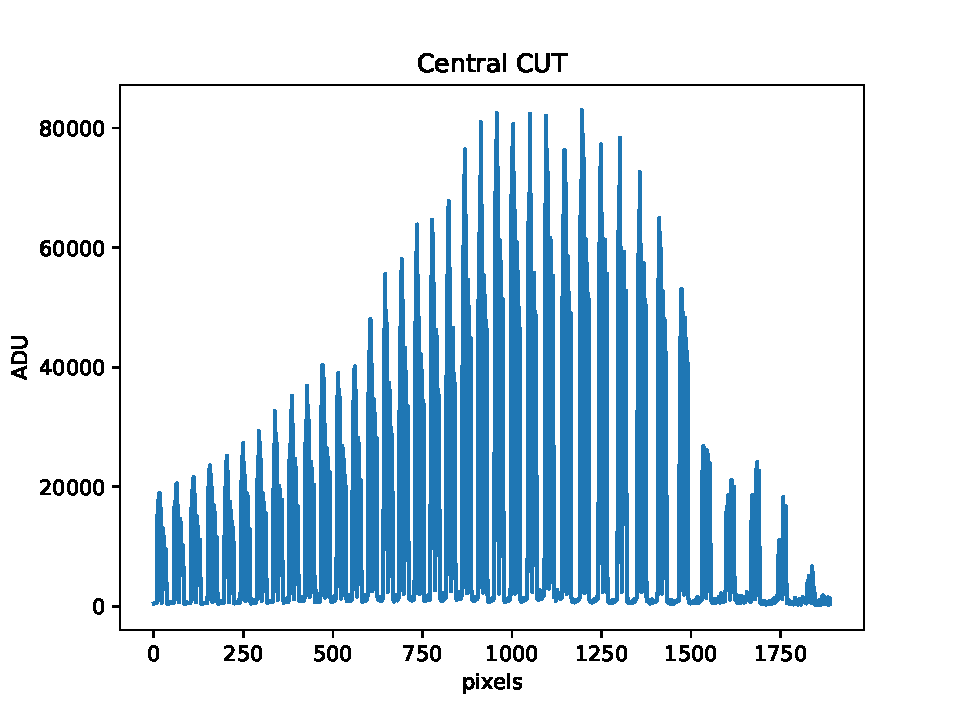
\includegraphics[width=\textwidth]{Figures/cal_loc_RAW_spirou_1.pdf}
a
\end{center}
\end{minipage}%
\begin{minipage}{.495\textwidth}
\begin{center}
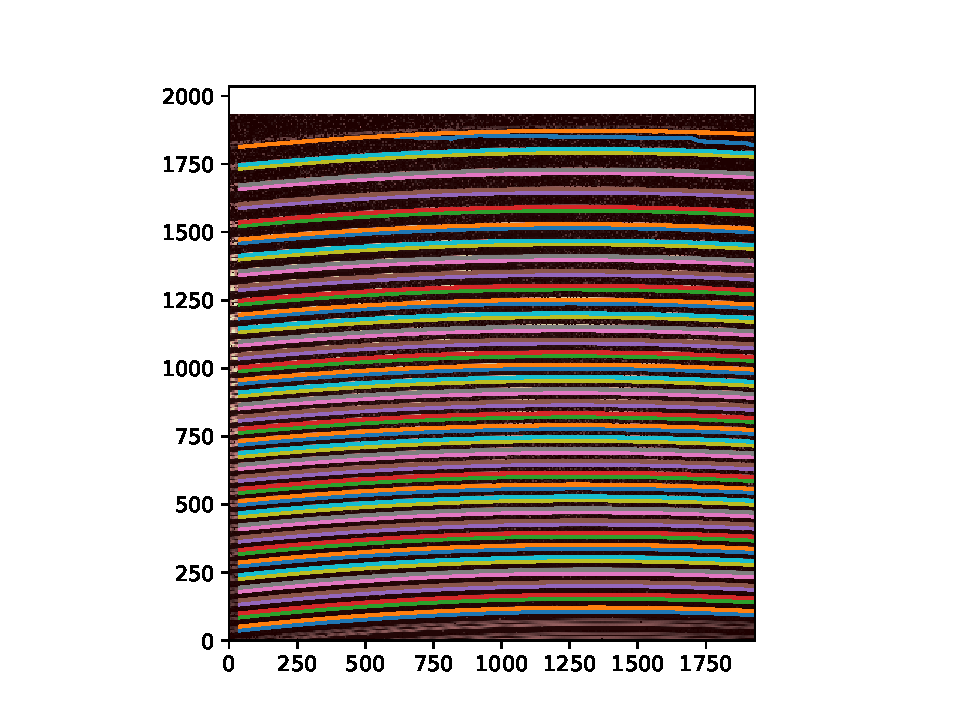
\includegraphics[width=\textwidth]{Figures/cal_loc_RAW_spirou_2.pdf}
b
\end{center}
\end{minipage}%
\end{center}

\begin{center}
\begin{minipage}{.495\textwidth}
\begin{center}
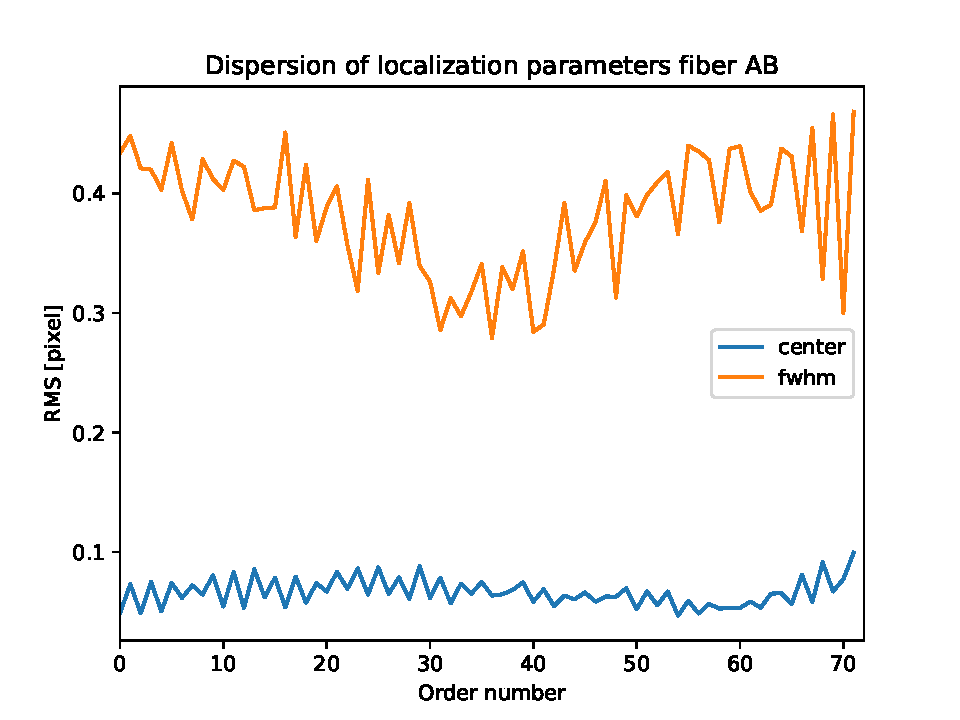
\includegraphics[width=\textwidth]{Figures/cal_loc_RAW_spirou_3.pdf}
c
\end{center}
\end{minipage}%
\end{center}

\caption{\textbf{(a)} Pixel number (across order) against flux value of central pixel. \textbf{(b)} Image with fits to each order. \textbf{(c)} The dispersion of localization parameters. \label{figure:cal_loc_RAW_spirou}}
\end{figure}


%%
\clearpage
\newpage
\section{The cal\_SLIT recipe}
\label{ch:the_recipes:cal_SLIT_spirou}
%%
%%%%%%%%%%%%%%%%%%%%%%%%%%%%%%%%%%%%%%%%%%%%%%%%%%%%%%%%

Fabry-Perot exposures in which the three fibres are simultaneously fed by light from the Fabry-Perot filter. Each exposure is used to build the slit orientation. Finds the tilt of the orders. \\

% -------------------------------------------------------
\subsection{The inputs}
% -------------------------------------------------------
The input of {\calSLIT} is as follows:
\begin{cmdbox}
cal_SLIT_spirou.py night_repository filenames
\end{cmdbox}
\noindent for example:
\begin{cmdbox}
cal_SLIT_spirou.py 20170710 fp_fp02a203.fits fp_fp03a203.fits fp_fp04a203.fits
\end{cmdbox}
\noindent or
\begin{pythonbox}
import cal_SLIT_spirou
night_repository = '20170710'
filenames = ['fp_fp02a203.fits', 'fp_fp03a203.fits', 'fp_fp04a203.fits']
cal_SLIT_spirou.main(night_repository, files=filenames)
\end{pythonbox}

\noindent where `night\_repository' defines \argnightname and `filenames' define the list of files in \argfilenames. All files in filenames must be valid python strings separated by a space (command line) or in a line (python) and must have the folowing prefixes:
\begin{itemize}
	\item fp\_fp
\end{itemize}

% -------------------------------------------------------
\subsection{The outputs}
% -------------------------------------------------------
The outputs of \calSLIT are as follows:

\begin{itemize}
\item \definevariable{text:tiltfits}{tiltfits} in form:
\begin{tcustomdir}
\{\reduceddir\}/\{date prefix\}\_\{file\}\_tilt.fits
\end{tcustomdir}

\end{itemize}

\noindent where `date prefix' is constructed from \argnightname and the file name is the first file in \argfilenames.

\noindent for example for \reduceddir\lstinline[style=pythoninline]|='/drs/data/reduced/20170710'| and \argfilenames\lstinline[style=pythoninline]|=['fp_fp02a203.fits', 'fp_fp03a203.fits', 'fp_fp04a203.fits']| the output files would be:
\begin{tcustomdir}
\begin{itemize}
\item \path{/drs/data/reduced/20170710/20170710_fp_fp02a203_tilt.fits}
\end{itemize}
\end{tcustomdir}

% -------------------------------------------------------
\subsection{Summary of procedure}
% -------------------------------------------------------
\begin{enumerate}
\item adds all fp\_fp files together
\item corrects for dark
\item resizes the image
\item extracts the orders (no weight no tilt)
\item works out the tilt for each order using the location and width
\item saves the tilt to file
\item should do some quality control
\item  updates calibDB with key ``TILT''
\end{enumerate}


% -------------------------------------------------------
\subsection{Quality Control}
% -------------------------------------------------------

There are currently two quality control checks for \calSLIT
\begin{itemize}

\item Abnormal RMS of SLIT angle if:
\begin{thighlight}
\begin{equation}
\text{RMS}_\text{tilt} > \text{\definevariable{text:qc_slit_rms}{qc\_slit\_rms}}
\end{equation}
\end{thighlight}

\item Abnormal SLIT angle if:
\begin{thighlight}
\begin{equation}
\text{max}(\text{tilt}) > \text{\definevariable{text:c_slit_max}{qc\_slit\_max}}
\end{equation}
or
\begin{equation}
\text{min}(\text{tilt}) < \text{\definevariable{text:c_slit_min}{qc\_slit\_min}}
\end{equation}
\end{thighlight}

\end{itemize}

\noindent If none of these quality control criteria are valid then the output file is passed into the \calibdb with key `TILT'. \\

\noindent For example the following lines are added to the \calibdb for 
\argnightname{\lstinline[style=pythoninline]| = "20170710" |} and \argfilenames{\lstinline[style=pythoninline]| = ['fp_fp02a203.fits', 'fp_fp03a203.fits', 'fp_fp04a203.fits'] |}. \\

\begin{textbox}[title={In calibration database file}]
TILT 20170710 20170710_fp_fp02a203_tilt.fits 2017-07-10-13:25:15.590000 1499693115.59
\end{textbox}


% -------------------------------------------------------
\subsection{Example working run}
% -------------------------------------------------------

An example run where everything worked is below:
\begin{cmdbox}
cal_SLIT_spirou.py 20170710 fp_fp02a203.fits fp_fp03a203.fits fp_fp04a203.fits
\end{cmdbox}
\begin{cmdboxprintspecial}[fontupper=\tiny, fontlower=\tiny]
@gHH:MM:SS.S -   || *****************************************@g
@gHH:MM:SS.S -   || * SPIROU \@(#) Geneva Observatory (VERSION)@g
@gHH:MM:SS.S -   || *****************************************@g
@gHH:MM:SS.S -   ||(dir_data_raw)      DRS_DATA_RAW=/scratch/Projects/spirou_py3/data/raw@g
@gHH:MM:SS.S -   ||(dir_data_reduc)    DRS_DATA_REDUC=/scratch/Projects/spirou_py3/data/reduced@g
@gHH:MM:SS.S -   ||(dir_calib_db)      DRS_CALIB_DB=/scratch/Projects/spirou_py3/data/calibDB@g
@gHH:MM:SS.S -   ||(dir_data_msg)      DRS_DATA_MSG=/scratch/Projects/spirou_py3/data/msg@g
@gHH:MM:SS.S -   ||(print_level)       PRINT_LEVEL=all         %(error/warning/info/all)@g
@gHH:MM:SS.S -   ||(log_level)         LOG_LEVEL=all         %(error/warning/info/all)@g
@gHH:MM:SS.S -   ||(plot_graph)        DRS_PLOT=1            %(def/undef/trigger)@g
@gHH:MM:SS.S -   ||(used_date)         DRS_USED_DATE=undefined@g
@gHH:MM:SS.S -   ||(working_dir)       DRS_DATA_WORKING=/scratch/Projects/spirou_py3/data/tmp@g
@gHH:MM:SS.S -   ||                    DRS_INTERACTIVE is not set, running on-line mode@g
@gHH:MM:SS.S -   ||                    DRS_DEBUG is set, debug mode level:1@g
@gHH:MM:SS.S -   |cal_SLIT_spirou:2a203+[...]|Now running : cal_SLIT_spirou on file(s): fp_fp02a203.fits, fp_fp03a203.fits, fp_fp04a203.fits@g
@gHH:MM:SS.S -   |cal_SLIT_spirou:2a203+[...]|On directory /scratch/Projects/spirou_py3/data/raw/20170710@g
@gHH:MM:SS.S -   |cal_SLIT_spirou:2a203+[...]|ICDP_NAME loaded from: /scratch/Projects/spirou_py3/spirou_py3/INTROOT/config/constants_SPIROU.py@g
@gHH:MM:SS.S - * |cal_SLIT_spirou:2a203+[...]|Correct type of image for slit (f or p or _ or f or p)@g
@gHH:MM:SS.S -   |cal_SLIT_spirou:2a203+[...]|Calibration file: 20170710_flat_flat02f10_badpixel.fits already exists - not copied@g
...
@gHH:MM:SS.S -   |cal_SLIT_spirou:2a203+[...]|Calibration file: spirou_wave_ini3.fits already exists - not copied@g
@gHH:MM:SS.S -   |cal_SLIT_spirou:2a203+[...]|Calibration file: 2017-10-11_21-32-17_hcone_hcone02c406_wave_AB.fits already exists - not copied@g
@gHH:MM:SS.S -   |cal_SLIT_spirou:2a203+[...]|Calibration file: spirou_wave_ini3.fits already exists - not copied@g
@gHH:MM:SS.S -   |cal_SLIT_spirou:2a203+[...]|Calibration file: 2017-10-11_21-32-17_hcone_hcone02c406_wave_C.fits already exists - not copied@g
@gHH:MM:SS.S - * |cal_SLIT_spirou:2a203+[...]|Now processing Image TYPE UNKNOWN with cal_SLIT_spirou recipe@g
@gHH:MM:SS.S -   |cal_SLIT_spirou:2a203+[...]|Reading Image /scratch/Projects/spirou_py3/data/raw/20170710/fp_fp02a203.fits@g
@gHH:MM:SS.S -   |cal_SLIT_spirou:2a203+[...]|Image 2048 x 2048 loaded@g
@gHH:MM:SS.S - * |cal_SLIT_spirou:2a203+[...]|Adding 2 frame(s)@g
@gHH:MM:SS.S -   |cal_SLIT_spirou:2a203+[...]|Reading File: /scratch/Projects/spirou_py3/data/raw/20170710/fp_fp03a203.fits@g
@gHH:MM:SS.S -   |cal_SLIT_spirou:2a203+[...]|Reading File: /scratch/Projects/spirou_py3/data/raw/20170710/fp_fp04a203.fits@g
@gHH:MM:SS.S -   |cal_SLIT_spirou:2a203+[...]|Doing Dark Correction using /scratch/Projects/spirou_py3/data/calibDB/20170710_dark_dark02d406.fits@g
@gHH:MM:SS.S -   |cal_SLIT_spirou:2a203+[...]|Image format changed to 1930x2035@g
@gHH:MM:SS.S - * |cal_SLIT_spirou:2a203+[...]|Nb dead pixels = 611716 / 15.58 %@g
@gHH:MM:SS.S -   |cal_SLIT_spirou:2a203+[...]|Reading localization parameters of Fiber AB@g
@gHH:MM:SS.S -   |cal_SLIT_spirou:2a203+[...]|Order 0.0: Tilt = 4.70 on pixel 37.0 = -7.23 deg@g
@gHH:MM:SS.S -   |cal_SLIT_spirou:2a203+[...]|Order 1.0: Tilt = 4.60 on pixel 37.4 = -7.02 deg@g
@gHH:MM:SS.S -   |cal_SLIT_spirou:2a203+[...]|Order 2.0: Tilt = 4.50 on pixel 36.8 = -6.97 deg@g
@gHH:MM:SS.S -   |cal_SLIT_spirou:2a203+[...]|Order 3.0: Tilt = 4.30 on pixel 36.3 = -6.75 deg@g
...
@gHH:MM:SS.S -   |cal_SLIT_spirou:2a203+[...]|Order 32.0: Tilt = 1.40 on pixel 33.3 = -2.41 deg@g
@gHH:MM:SS.S -   |cal_SLIT_spirou:2a203+[...]|Order 33.0: Tilt = 1.10 on pixel 32.3 = -1.95 deg@g
@gHH:MM:SS.S -   |cal_SLIT_spirou:2a203+[...]|Order 34.0: Tilt = 1.00 on pixel 32.1 = -1.79 deg@g
@gHH:MM:SS.S -   |cal_SLIT_spirou:2a203+[...]|Order 35.0: Tilt = 0.30 on pixel 17.1 = -1.01 deg@g
@gHH:MM:SS.S - * |cal_SLIT_spirou:2a203+[...]AB|Tilt dispersion = 0.091 deg@g
@gHH:MM:SS.S -   |cal_SLIT_spirou:2a203+[...]|Saving tilt  information in file: 20170710_fp_fp02a203_tilt.fits@g
@yHH:MM:SS.S - \@ |python warning Line 980  warning reads: Card is too long, comment will be truncated.|@y
@gHH:MM:SS.S - * |cal_SLIT_spirou:2a203+[...]|QUALITY CONTROL SUCCESSFUL - Well Done -@g
@gHH:MM:SS.S - * |cal_SLIT_spirou:2a203+[...]|Updating Calib Data Base with TILT@g
@gHH:MM:SS.S - * |cal_SLIT_spirou:2a203+[...]|Recipe cal_SLIT_spirou has been successfully completed@gHHMSSS
\end{cmdboxprintspecial}

% -------------------------------------------------------
\newpage
\subsection{Interactive mode}
% -------------------------------------------------------

\noindent In interactive mode three figures will also appear (see Figure \ref{figure:cal_SLIT_spirou}).

\begin{figure}

\begin{center}
\begin{minipage}{.495\textwidth}
\begin{center}
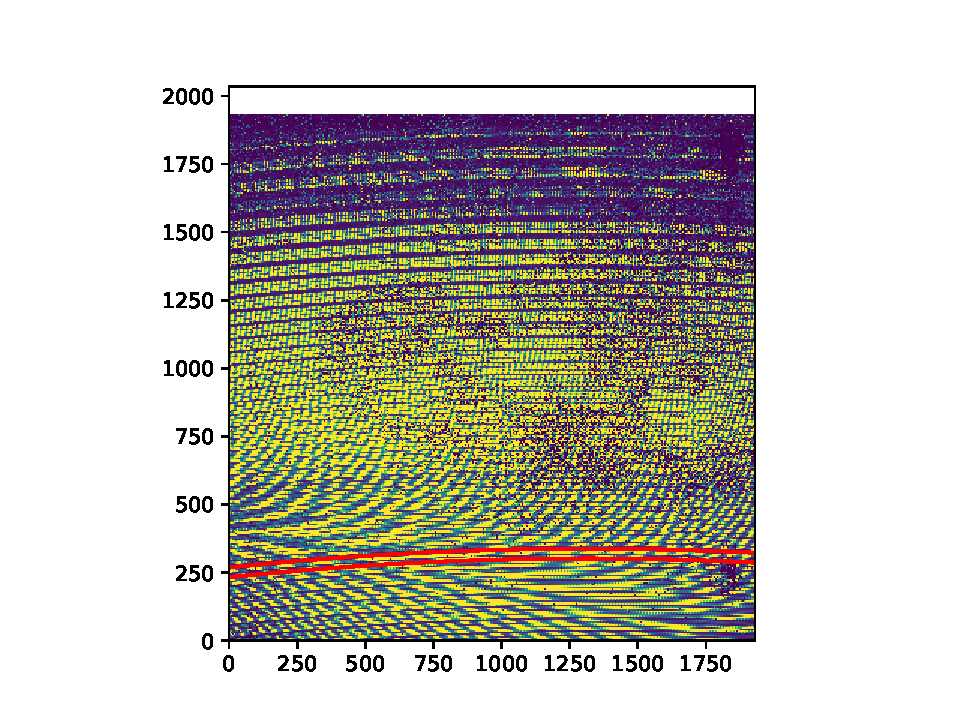
\includegraphics[width=\textwidth]{Figures/cal_SLIT_spirou_1a.pdf}
a
\end{center}
\end{minipage}%
\begin{minipage}{.495\textwidth}
\begin{center}
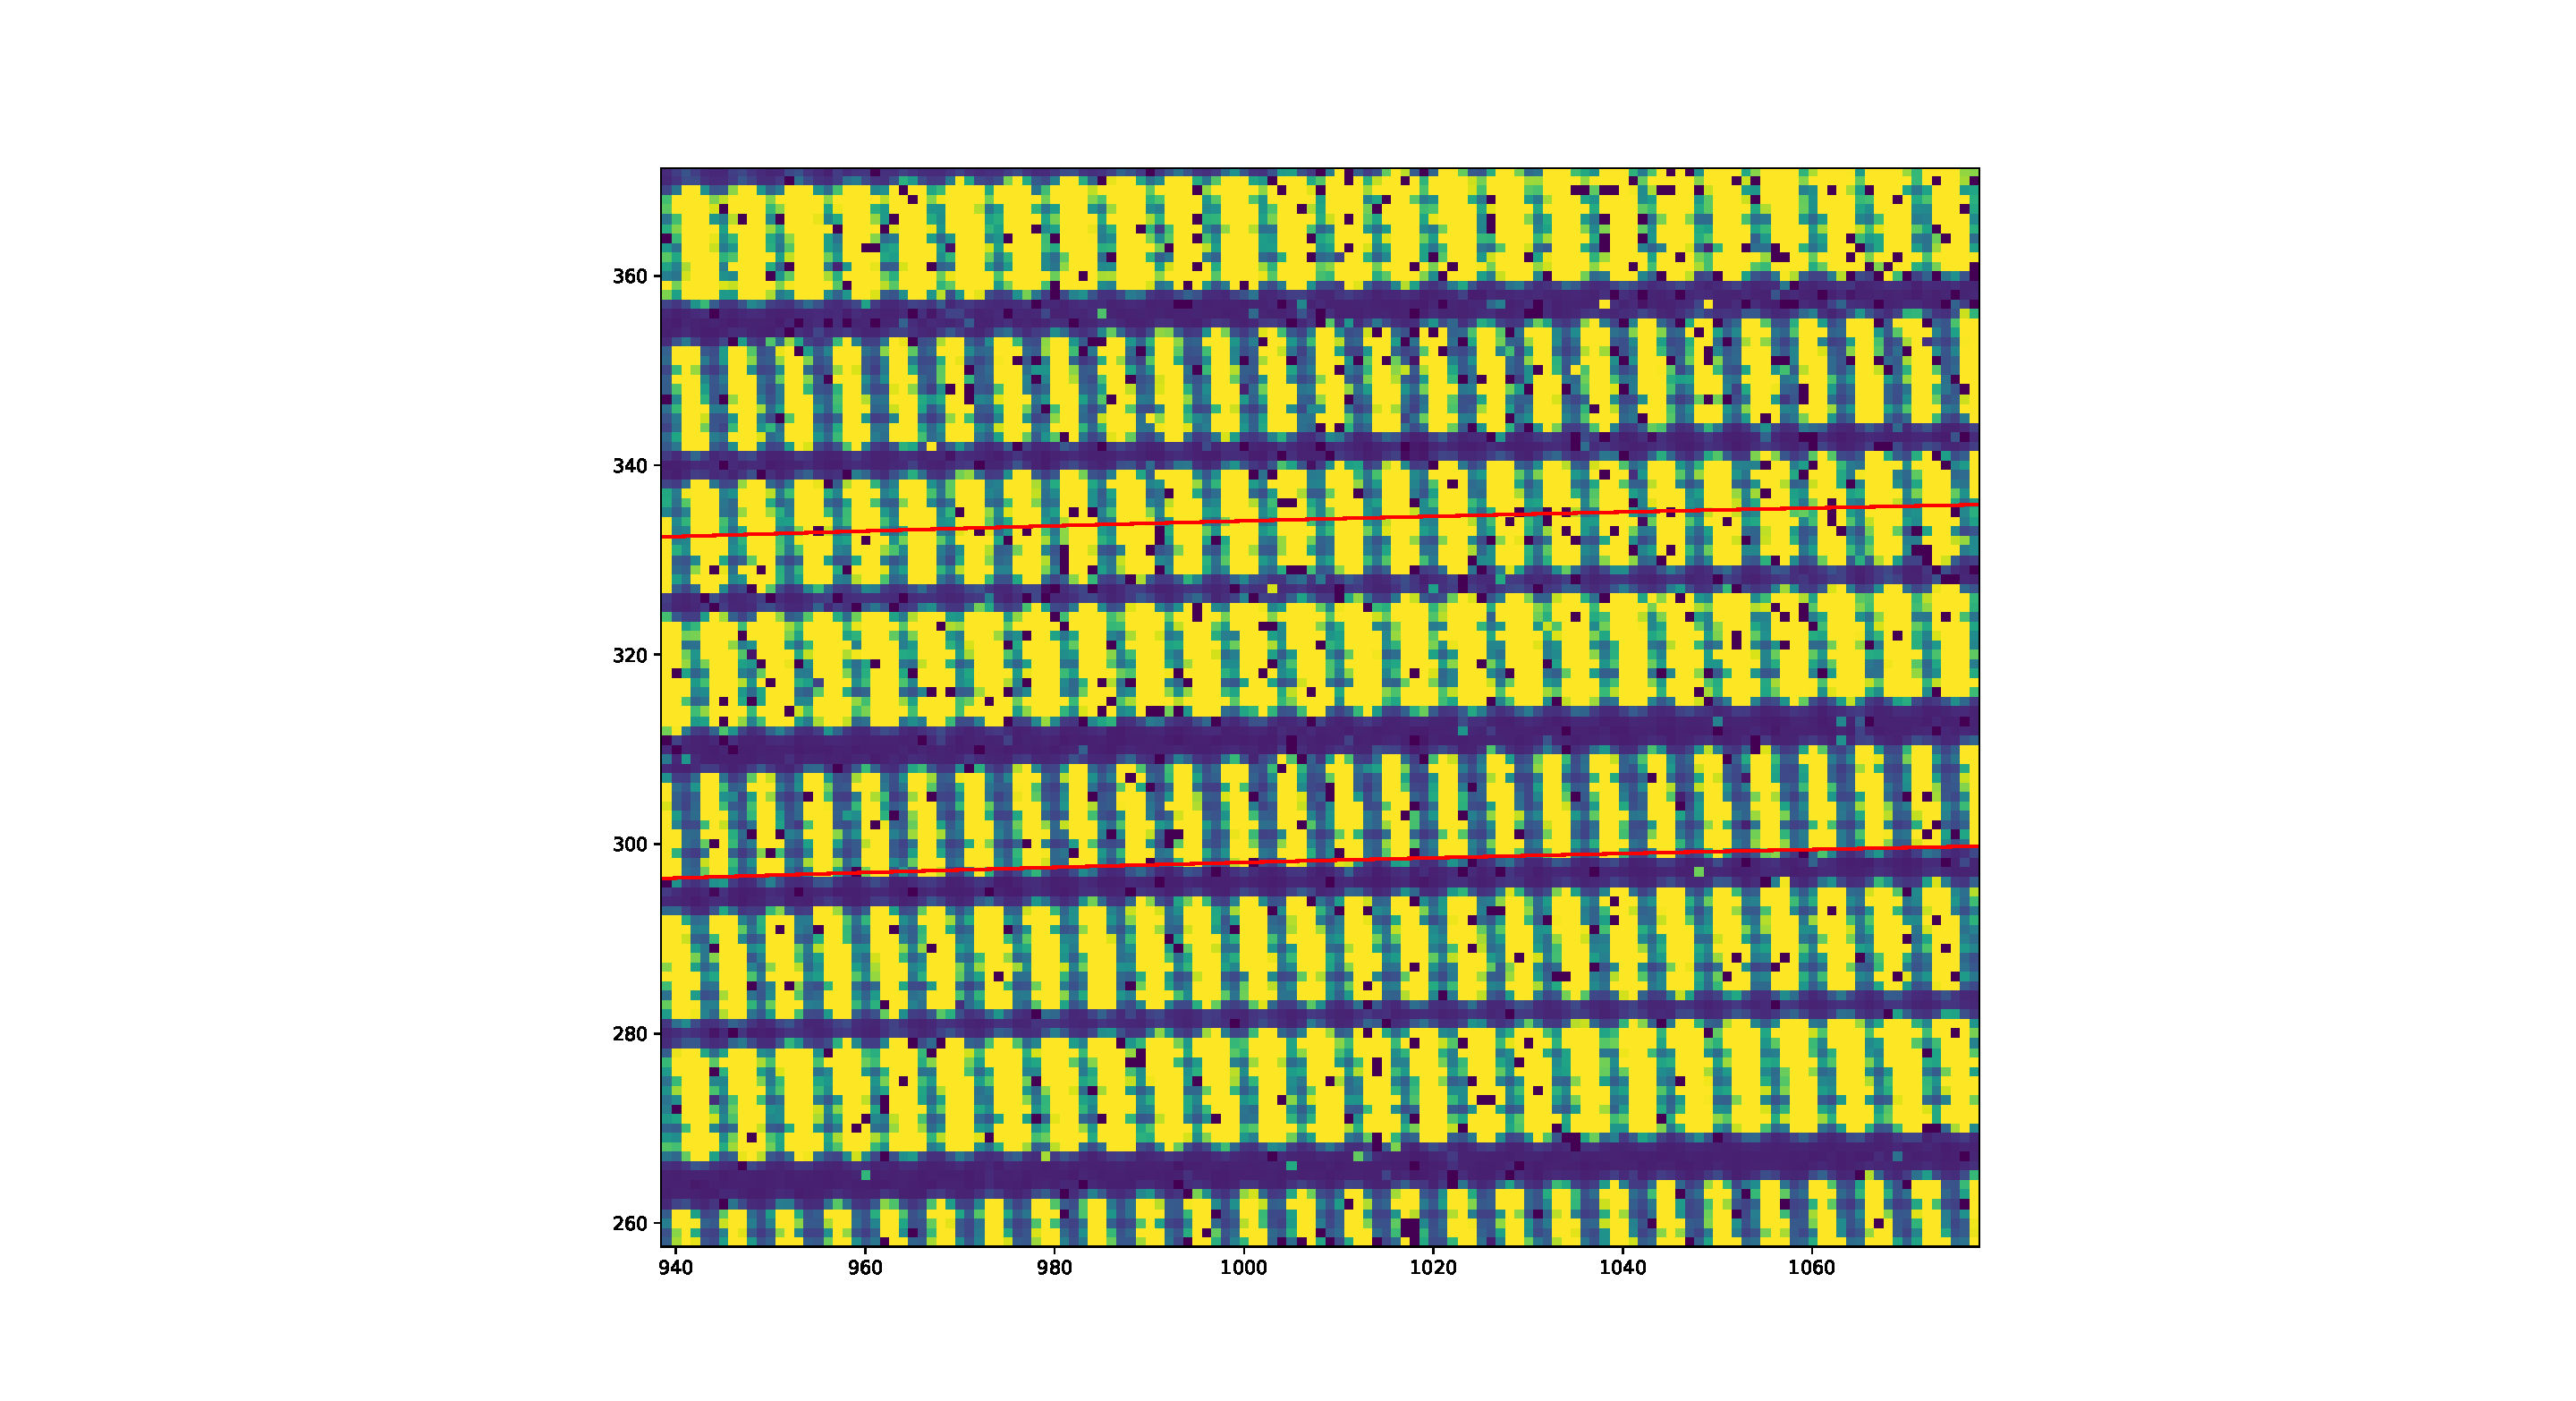
\includegraphics[width=\textwidth]{Figures/cal_SLIT_spirou_1b.pdf}
b
\end{center}
\end{minipage}%
\end{center}

\begin{center}
\begin{minipage}{.495\textwidth}
\begin{center}
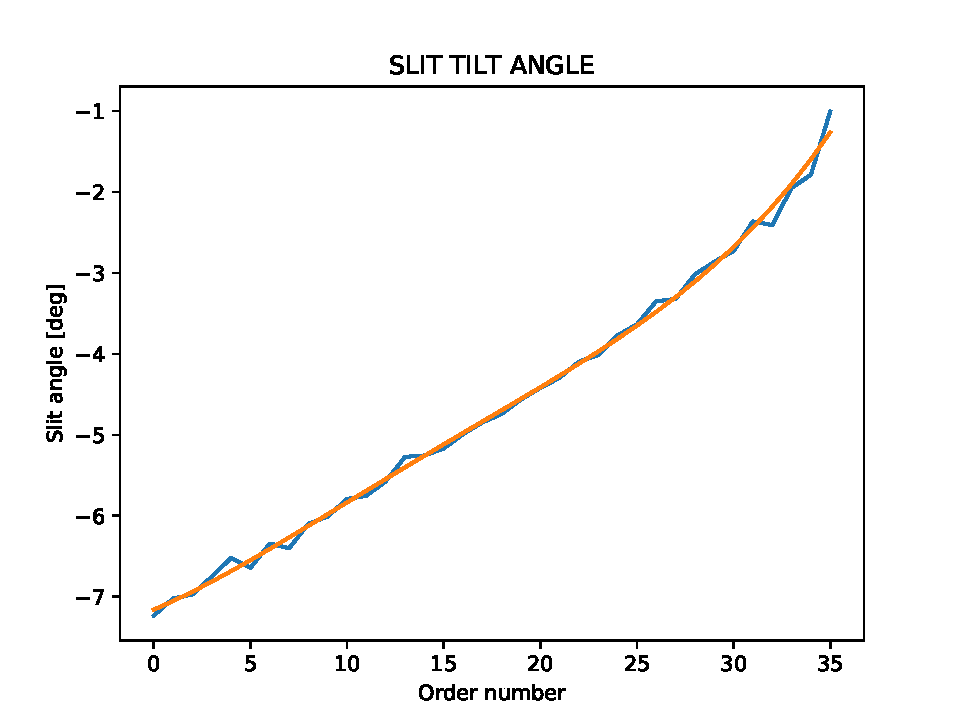
\includegraphics[width=\textwidth]{Figures/cal_SLIT_spirou_2.pdf}
c
\end{center}
\end{minipage}%
\end{center}

\caption{\textbf{(a)} The full `fp\_fp' image with one orders fit plotted. \textbf{(b)} Zoom in on a section of the `fp\_fp' image showing the tilt. \textbf{(c)} Slit aginle as a function of order number with the fit to the tilt also show. \label{figure:cal_SLIT_spirou}}
\end{figure}

%%%%%%%%%%%%%%%%%%%%%%%%%%%%%%%%%%%%%%%%%%%%%%%%%%%%%%%%
%%
\clearpage
\newpage
\section{The cal\_FF recipe}
\label{ch:the_recipes:cal_FF_RAW_spirou}
%%
%%%%%%%%%%%%%%%%%%%%%%%%%%%%%%%%%%%%%%%%%%%%%%%%%%%%%%%%

Creates the flat fields. \\ 

% -------------------------------------------------------
\subsection{The inputs}
% -------------------------------------------------------
The input of \calFFraw is as follows:
\begin{cmdbox}
cal_FF_RAW_spirou.py night_repository filenames
\end{cmdbox}
\noindent for example
\begin{cmdbox}[title={example}]
cal_FF_RAW_spirou.py 20170710 dark_flat02f10.fits dark_flat03f10.fits dark_flat04f10.fits dark_flat05f10.fits dark_flat06f10.fits
\end{cmdbox}
\noindent or
\begin{pythonbox}
import cal_FF_RAW_spirou
night_repository = '20170710'
filenames = ['dark_flat02f10.fits', 'dark_flat03f10.fits', 'dark_flat04f10.fits', 
             'dark_flat05f10.fits', 'dark_flat06f10.fits']
cal_FF_RAW_spirou.main()
\end{pythonbox}

\noindent where `night\_repository' defines \argnightname and `filenames' define the list of files in \argfilenames. All files in filenames must be valid python strings separated by a space (command line) or in a line (python) and must have the folowing prefixes:
\begin{itemize}
	\item dark\_flat
	\item flat\_dark
\end{itemize}

% -------------------------------------------------------
\subsection{The outputs}
% -------------------------------------------------------
The outputs of \calFFraw are as follows:

\begin{itemize}

\item \definevariable{text:blazefits}{blazefits} in form:
\begin{tcustomdir}
\{\reduceddir\}/\{date prefix\}\_\{file\}\_blaze\_\{fiber\}.fits
\end{tcustomdir}

\item \definevariable{text:flatfits}{flatfits} in form:
\begin{tcustomdir}
\{\reduceddir\}/\{date prefix\}\_\{file\}\_flat\_\{fiber\}.fits
\end{tcustomdir}

\end{itemize}


\noindent where `date prefix' is constructed from \argnightname and the file name is the first file in \argfilenames.


\noindent for example for \reduceddir\lstinline[style=pythoninline]|='/drs/data/reduced/20170710'| and \argfilenames\lstinline[style=pythoninline]|=['dark_flat02f10.fits', 'dark_flat03f10.fits', 'dark_flat04f10.fits', 'dark_flat05f10.fits', 'dark_flat06f10.fits']| the output files would be:
\begin{tcustomdir}
\begin{itemize}
\item \path{/drs/data/reduced/20170710/20170710_flat_dark02f10_blaze_AB.fits}
\item \path{/drs/data/reduced/20170710/20170710_flat_dark02f10_flat_AB.fits}
\end{itemize}
\end{tcustomdir}

% -------------------------------------------------------
\subsection{Summary of procedure}
% -------------------------------------------------------
\begin{enumerate}
\item adds all `dark\_flat' or `flat\_dark' files together
\item corrects for darks
\item resizes the image
\item possible background subtraction?
\item extracts the orders using tilt and weight
\item calculates the blaze
\item calculates the flat field, (flat = extraction / blaze)
\item stores the flat fields
\item does some quality control
\item updates calibDB with key "FLAT\_\{fiber\}" where \{fiber\} = [AB, C] etc
\end{enumerate}

% -------------------------------------------------------
\subsection{Quality Control}
% -------------------------------------------------------

There is currently one quality control check for \calFFraw
\begin{itemize}
\item Too much flux in the image: 
\begin{thighlight}
\begin{equation}
\text{maximum signal} > \text{\definevariable{text:qc_max_signal}{qc\_max\_signal}} * \text{\definevariable{text:nbframes}{nbframes}}
\end{equation}
\end{thighlight}
\end{itemize}
\begin{note}
This check does not currently lead to a failed run and all files are processed as passing quality checks
\end{note}

\noindent The output file is passed into the \calibdb with key `FLAT\_\{fiber\}' for the `\definevariable{text:flatfits}{flatfits}' file. \\

\noindent For example the following lines are added to the \calibdb for 
\argnightname{\lstinline[style=pythoninline]| = "20170710" |} and \argfilenames{\lstinline[style=pythoninline]|=['dark_flat02f10.fits', 'dark_flat03f10.fits', 'dark_flat04f10.fits', 'dark_flat05f10.fits', 'dark_flat06f10.fits']|}. \\

\begin{textbox}[title={In calibration database file}]
FLAT_C 20170710 20170710_dark_flat02f10_flat_C.fits 2017-07-10-13:03:50.440000 1499691830.44
BLAZE_C 20170710 20170710_dark_flat02f10_blaze_C.fits 2017-07-10-13:03:50.440000 1499691830.44
\end{textbox}


% -------------------------------------------------------
\newpage
\subsection{Example working run}
% -------------------------------------------------------

An example run where everything worked is below:
\begin{cmdbox}[title={example}]
cal_FF_RAW_spirou.py 20170710 dark_flat02f10.fits dark_flat03f10.fits dark_flat04f10.fits dark_flat05f10.fits dark_flat06f10.fits
\end{cmdbox}
\begin{cmdboxprintspecial}[fontupper=\tiny, fontlower=\tiny]
@gHH:MM:SS.S -   || *****************************************@g
@gHH:MM:SS.S -   || * SPIROU \@(#) Geneva Observatory (VERSION)@g
@gHH:MM:SS.S -   || *****************************************@g
@gHH:MM:SS.S -   ||(dir_data_raw)      DRS_DATA_RAW=/drs/data/raw@g
@gHH:MM:SS.S -   ||(dir_data_reduc)    DRS_DATA_REDUC=/drs/data/reduced@g
@gHH:MM:SS.S -   ||(dir_calib_db)      DRS_CALIB_DB=/drs/data/calibDB@g
@gHH:MM:SS.S -   ||(dir_data_msg)      DRS_DATA_MSG=/drs/data/msg@g
@gHH:MM:SS.S -   ||(print_level)       PRINT_LEVEL=all         %(error/warning/info/all)@g
@gHH:MM:SS.S -   ||(log_level)         LOG_LEVEL=all         %(error/warning/info/all)@g
@gHH:MM:SS.S -   ||(plot_graph)        DRS_PLOT=1            %(def/undef/trigger)@g
@gHH:MM:SS.S -   ||(used_date)         DRS_USED_DATE=undefined@g
@gHH:MM:SS.S -   ||(working_dir)       DRS_DATA_WORKING=/drs/data/tmp@g
@gHH:MM:SS.S -   ||                    DRS_INTERACTIVE is not set, running on-line mode@g
@gHH:MM:SS.S -   ||                    DRS_DEBUG is set, debug mode level:1@g
@gHH:MM:SS.S -   |cal_FF_RAW_spirou:02f10+[...]|Now running : cal_FF_RAW_spirou on file(s): dark_flat02f10.fits, dark_flat03f10.fits, dark_flat04f10.fits, dark_flat05f10.fits, dark_flat06f10.fits@g
@gHH:MM:SS.S -   |cal_FF_RAW_spirou:02f10+[...]|On directory /drs/data/raw/20170710@g
@gHH:MM:SS.S -   |cal_FF_RAW_spirou:02f10+[...]|ICDP_NAME loaded from: /scratch/Projects/spirou_py3/spirou_py3/INTROOT/config/constants_SPIROU.py@g
@gHH:MM:SS.S - * |cal_FF_RAW_spirou:02f10+[...]|Correct type of image for Flat-field (dark_flat or flat_dark)@g
@gHH:MM:SS.S -   |cal_FF_RAW_spirou:02f10+[...]|Calibration file: 20170710_flat_flat02f10_badpixel.fits already exists - not copied@g
@gHH:MM:SS.S -   |cal_FF_RAW_spirou:02f10+[...]|Calibration file: 20170710_dark_dark02d406.fits already exists - not copied@g
...
@gHH:MM:SS.S -   |cal_FF_RAW_spirou:02f10+[...]|Calibration file: 20170710_flat_dark02f10_order_profile_AB.fits already exists - not copied@g
@gHH:MM:SS.S -   |cal_FF_RAW_spirou:02f10+[...]|Calibration file: 20170710_dark_flat02f10_order_profile_C.fits already exists - not copied@g
@gHH:MM:SS.S -   |cal_FF_RAW_spirou:02f10+[...]|Calibration file: 20170710_fp_fp02a203_tilt.fits already exists - not copied@g
@gHH:MM:SS.S -   |cal_FF_RAW_spirou:02f10+[...]|Calibration file: spirou_wave_ini3.fits already exists - not copied@g
@gHH:MM:SS.S -   |cal_FF_RAW_spirou:02f10+[...]|Calibration file: 2017-10-11_21-32-17_hcone_hcone02c406_wave_AB.fits already exists - not copied@g
@gHH:MM:SS.S -   |cal_FF_RAW_spirou:02f10+[...]|Calibration file: spirou_wave_ini3.fits already exists - not copied@g
@gHH:MM:SS.S -   |cal_FF_RAW_spirou:02f10+[...]|Calibration file: 2017-10-11_21-32-17_hcone_hcone02c406_wave_C.fits already exists - not copied@g
@gHH:MM:SS.S - * |cal_FF_RAW_spirou:02f10+[...]|Now processing Image TYPE UNKNOWN with cal_FF_RAW_spirou recipe@g
@gHH:MM:SS.S -   |cal_FF_RAW_spirou:02f10+[...]|Reading Image /drs/data/raw/20170710/dark_flat02f10.fits@g
@gHH:MM:SS.S -   |cal_FF_RAW_spirou:02f10+[...]|Image 2048 x 2048 loaded@g
@gHH:MM:SS.S - * |cal_FF_RAW_spirou:02f10+[...]|Adding 4 frame(s)@g
@gHH:MM:SS.S -   |cal_FF_RAW_spirou:02f10+[...]|Reading File: /drs/data/raw/20170710/dark_flat03f10.fits@g
@gHH:MM:SS.S -   |cal_FF_RAW_spirou:02f10+[...]|Reading File: /drs/data/raw/20170710/dark_flat04f10.fits@g
@gHH:MM:SS.S -   |cal_FF_RAW_spirou:02f10+[...]|Reading File: /drs/data/raw/20170710/dark_flat05f10.fits@g
@gHH:MM:SS.S -   |cal_FF_RAW_spirou:02f10+[...]|Reading File: /drs/data/raw/20170710/dark_flat06f10.fits@g
@gHH:MM:SS.S -   |cal_FF_RAW_spirou:02f10+[...]|Doing Dark Correction using /drs/data/calibDB/20170710_dark_dark02d406.fits@g
@gHH:MM:SS.S -   |cal_FF_RAW_spirou:02f10+[...]|Image format changed to 2035x1930@g
@gHH:MM:SS.S - * |cal_FF_RAW_spirou:02f10+[...]|Nb dead pixels = 568541 / 14.48 %@g
@gHH:MM:SS.S - * |cal_FF_RAW_spirou:02f10+[...]|Maximum average flux/pixel in the spectrum: 73636.3 [ADU]@g
@gHH:MM:SS.S -   |cal_FF_RAW_spirou:02f10+[...]|Reading localization parameters of Fiber C@g
@gHH:MM:SS.S -   |cal_FF_RAW_spirou:02f10+[...]C|Reading order profile of Fiber C@g
@gHH:MM:SS.S -   |cal_FF_RAW_spirou:02f10+[...]|On fiber C order 0: S/N= 1158.4  - FF rms=4.68 %@g
@gHH:MM:SS.S -   |cal_FF_RAW_spirou:02f10+[...]|On fiber C order 1: S/N= 1193.9  - FF rms=4.80 %@g
@gHH:MM:SS.S -   |cal_FF_RAW_spirou:02f10+[...]|On fiber C order 2: S/N= 1232.6  - FF rms=4.76 %@g
...
@gHH:MM:SS.S -   |cal_FF_RAW_spirou:02f10+[...]|On fiber C order 33: S/N= 1686.9  - FF rms=5.67 %@g
@gHH:MM:SS.S -   |cal_FF_RAW_spirou:02f10+[...]|On fiber C order 34: S/N= 1574.5  - FF rms=8.17 %@g
@gHH:MM:SS.S -   |cal_FF_RAW_spirou:02f10+[...]|On fiber C order 35: S/N= 1260.6  - FF rms=8.10 %@g
@gHH:MM:SS.S -   |cal_FF_RAW_spirou:02f10+[...]C|Saving blaze spectrum for fiber: C in 20170710_dark_flat02f10_blaze_C.fits@g
@yHH:MM:SS.S - \@ |python warning Line 980  warning reads: Card is too long, comment will be truncated.|@y
@gHH:MM:SS.S -   |cal_FF_RAW_spirou:02f10+[...]C|Saving FF spectrum for fiber: C in 20170710_dark_flat02f10_flat_C.fits@g
@yHH:MM:SS.S - \@ |python warning Line 980  warning reads: Card is too long, comment will be truncated.|@y
@gHH:MM:SS.S - * |cal_FF_RAW_spirou:02f10+[...]|QUALITY CONTROL SUCCESSFUL - Well Done -@g
@gHH:MM:SS.S - * |cal_FF_RAW_spirou:02f10+[...]|Updating Calib Data Base with FLAT_C@g
@gHH:MM:SS.S - * |cal_FF_RAW_spirou:02f10+[...]|Updating Calib Data Base with BLAZE_C@g
@gHH:MM:SS.S - * |cal_FF_RAW_spirou:02f10+[...]|Recipe cal_FF_RAW_spirou has been successfully completed@g

\end{cmdboxprintspecial}


% -------------------------------------------------------
\newpage
\subsection{Interactive mode}
% -------------------------------------------------------

\noindent In interactive mode three figures will also appear (see Figure \ref{figure:cal_FF_raw_spirou}).

\begin{figure}

\begin{center}
\begin{minipage}{.495\textwidth}
\begin{center}
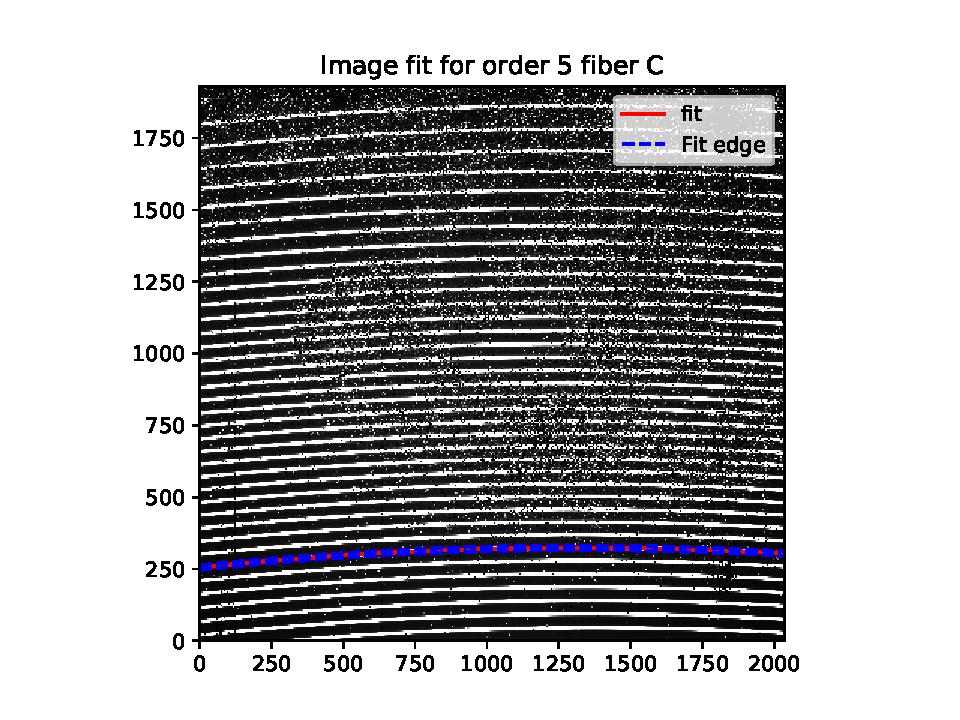
\includegraphics[width=\textwidth]{Figures/cal_FF_raw_spirou_1.pdf}
a
\end{center}
\end{minipage}%
\begin{minipage}{.495\textwidth}
\begin{center}
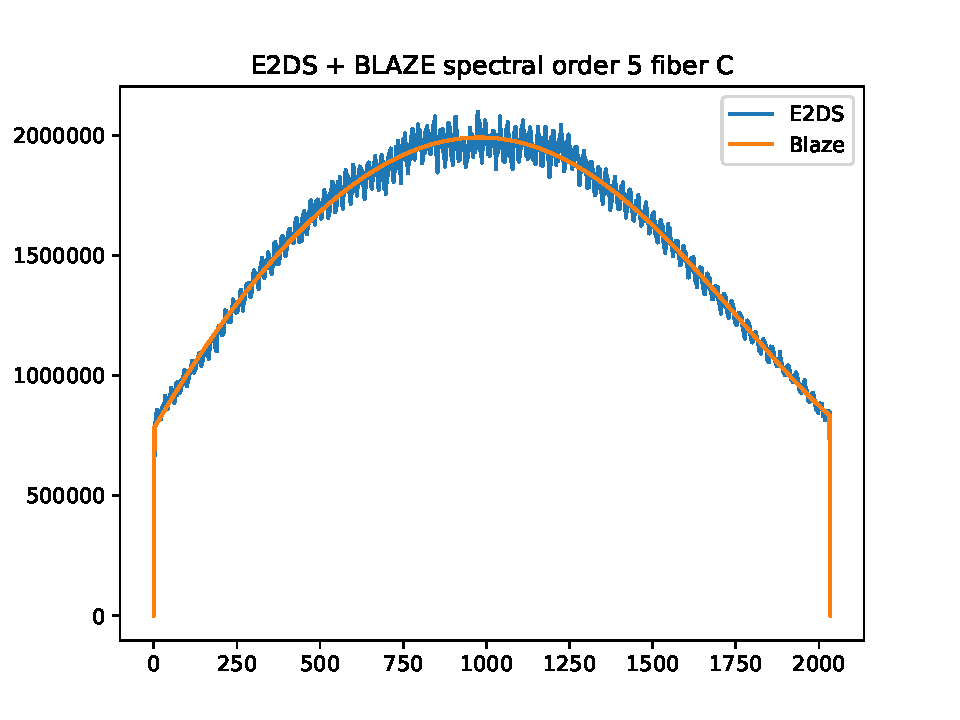
\includegraphics[width=\textwidth]{Figures/cal_FF_raw_spirou_2.pdf}
b
\end{center}
\end{minipage}%
\end{center}

\begin{center}
\begin{minipage}{.495\textwidth}
\begin{center}
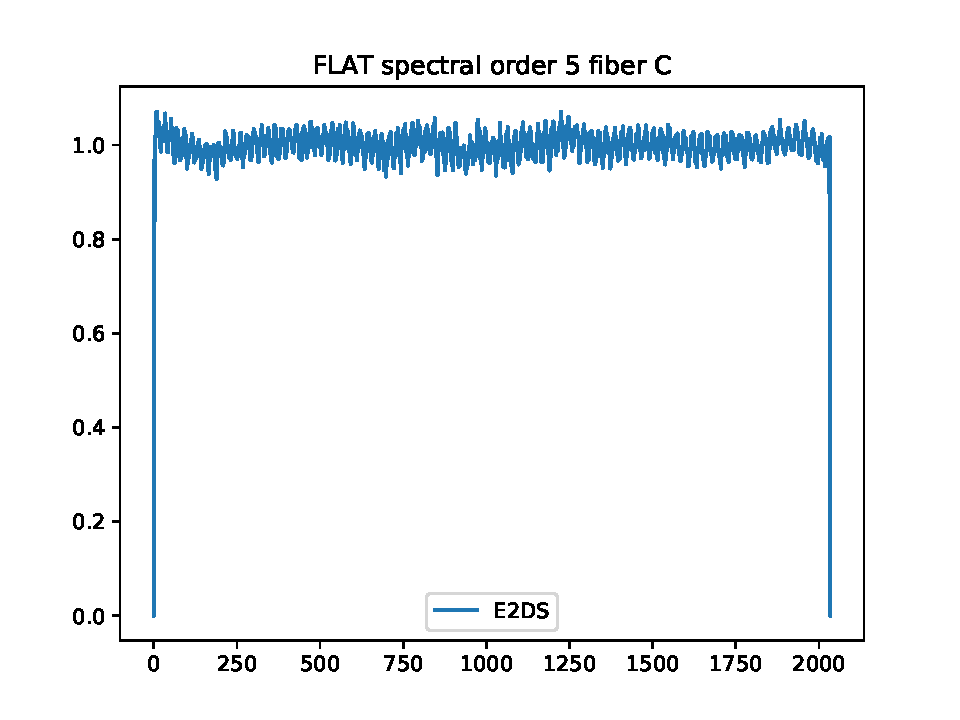
\includegraphics[width=\textwidth]{Figures/cal_FF_raw_spirou_3.pdf}
c
\end{center}
\end{minipage}%
\end{center}

\caption{\textbf{(a)} the full processed image with one order fit highlighted. \textbf{(b)} An extracted overplotted with the blaze fit. \textbf{(c)}  A flattened order. \label{figure:cal_FF_raw_spirou}}
\end{figure}

%%%%%%%%%%%%%%%%%%%%%%%%%%%%%%%%%%%%%%%%%%%%%%%%%%%%%%%%
%%
\clearpage
\newpage
\section{The cal\_extract recipes}
\label{ch:the_recipes:cal_extract_RAW_spirou}
%%
%%%%%%%%%%%%%%%%%%%%%%%%%%%%%%%%%%%%%%%%%%%%%%%%%%%%%%%%

Extracts orders for specific fibers and files. There are currently three extraction recipes. There is the main extraction recipe (\calextractRAW) and two wrapper recipes (\calextractRAWAB and \calextractRAWC, which push certain options into \calextractRAW).

% -------------------------------------------------------
\subsection{The inputs}
% -------------------------------------------------------
The input of \calextractRAW is as follows:
\begin{cmdbox}
cal_extract_RAW_spirou.py night_repository filenames
\end{cmdbox}
\noindent for example
\begin{cmdbox}[title={example}]
cal_extract_RAW_spirou.py 20170710 fp_fp02a203.fits
\end{cmdbox}
\noindent or
\begin{pythonbox}
import cal_extract_RAW_spirou
night_repository = '20170710'
filenames = ['fp_fp02a203.fits']
cal_extract_RAW_spirou.main(night_repository, files=filenames)
\end{pythonbox}

\noindent where `night\_repository' defines \argnightname and `filenames' define the list of files in \argfilenames. In addition to this one can add optional arguments (and this is the case for the wrapper recipes of \calextractRAWAB and \calextractRAWC). \\

\noindent All files in filenames must be valid python strings separated by a space (command line) or in a line (python) and should have the following prefixes:
\begin{itemize}
	\item fp\_fp
	\item hcone\_dark
	\item dark\_hcone
	\item hcone\_hcone
	\item dark\_dark\_AHC1
	\item dark\_hctwo
	\item hctwo\_hctwo
	\item dark\_dark\_AHC2
\end{itemize}

\subsubsection{Optional arguments}

By default \calextractRAW will extract all fibers defined in \definevariable{text:fiber_types}{fiber\_types} (i.e. `AB', `A', `B' and `C'). It may be the case that one wishes to extract only one fiber, this can be done by setting the `fiber\_type' option (when run from python). For example:
\begin{pythonbox}
import cal_extract_RAW_spirou
night_repository = '20170710'
filenames = ['fp_fp02a203.fits']
cal_DARK_spirou.main(night_repository, filenames, fiber_type='A')
\end{pythonbox}
\noindent where `fiber\_type' must be a valid python string and defined in \definevariable{text:fiber_types}{fiber\_types}. On can also overwrite any other variable that is (or even is not) defined in any of the constant files (or run time) by simply adding it as an optional argument in the python function call:
\begin{pythonbox}
import cal_extract_RAW_spirou
night_repository = '20170710'
filenames = ['fp_fp02a203.fits', 'fp_fp03a203.fits', 'fp_fp04a203.fits']
kwargs = dict(parameter1='This', parameter2='That')
cal_DARK_spirou.main(night_repository, filenames, fiber_type='A', **kwargs)
\end{pythonbox}
\begin{note}
This will extract fiber `A' and also set the values \lstinline[style=pythoninline]|parameter1='This'| and \lstinline[style=pythoninline]|parameter2='That'| in the main constant parameter dictionary.
\end{note}
\noindent This is the case for the two wrapper recipes (\calextractRAWAB and \calextractRAWC) which add some specific keywords that are used to individually extract fibers `AB' and `C' respectively. The two calls to the main extraction code are shown below but can be called from the console or python as with all other recipes.
\begin{cmdbox}
cal_extract_RAW_spirouAB.py night_repository filenames
cal_extract_RAW_spirouC.py night_repository filenames
\end{cmdbox}
\noindent for example
\begin{cmdbox}[title={example}]
cal_extract_RAW_spirouAB.py 20170710 fp_fp02a203.fits fp_fp03a203.fits fp_fp04a203.fits
cal_extract_RAW_spirouC.py 20170710 fp_fp02a203.fits fp_fp03a203.fits fp_fp04a203.fits
\end{cmdbox}
\noindent or
\begin{pythonbox}
import cal_extract_RAW_spirouAB
import cal_extract_RAW_spirouC
night_repository = '20170710'
filenames = ['fp_fp02a203.fits']
# extract fiber AB
cal_extract_RAW_spirouAB.main(night_repository, files=filenames)
# extract fiber C
cal_extract_RAW_spirouC.main(night_repository, files=filenames)
\end{pythonbox}
\noindent as mentioned above this can also be done in python just by adding additional arguments to \calextractRAW:
\begin{pythonbox}
import cal_extract_RAW_spirou
night_repository = '20170710'
filenames = ['fp_fp02a203.fits', 'fp_fp03a203.fits', 'fp_fp04a203.fits']
# extract fiber AB (for all extraction types)
cal_extract_RAW_spirou.main(night_repository, files=filenames,fiber_type='AB',
                            ic_extract_type='all', ic_ext_sigdet=-1)
# extract fiber C (for all extraction types)
cal_extract_RAW_spirou.main(night_repository, files=filenames,fiber_type='C',
                            ic_extract_type='all', ic_ext_sigdet=-1)
\end{pythonbox}
\begin{note}
Here we set the optional arguments \lstinline[style=pythoninline]|ic_extract_type='all', ic_ext_sigdet=-1|. \definevariable{text:ic_extract_type}{ic\_extract\_type} defines which type of extraction should be used (simple, tilt, weigh, tiltweight, all) and \definevariable{text:ic_ext_sigdet}{ic\_ext\_sigdet} manually sets the extraction sigdet (-1 sets it to the value from the HEADER else it is defined in \constantsfile).
\end{note}
\noindent The above python code is exactly what \calextractRAWAB and \calextractRAWC do by default.


% -------------------------------------------------------
\subsection{The outputs}
% -------------------------------------------------------
The outputs of \calextractRAW depend on the extraction type (\definevariable{text:ic_extract_type}{ic\_extract\_type}). 

\begin{itemize}

\item \definevariable{text:e2ds_file}{e2ds} in form:
\begin{tcustomdir}
\{\reduceddir\}/\{date prefix\}\_\{file\}\_e2ds\_\{fiber\}.fits
\end{tcustomdir}

\item \definevariable{text:exfitslist}{simple} in form:
\begin{tcustomdir}
\{\reduceddir\}/\{date prefix\}\_\{file\}\_e2ds\_\{fiber\}\_simple.fits
\end{tcustomdir}
\begin{note}
Only if \definevariable{text:ic_extract_type}{ic\_extract\_type} is `all'
\end{note}

\item \definevariable{text:exfitslist}{tilt} in form:
\begin{tcustomdir}
\{\reduceddir\}/\{date prefix\}\_\{file\}\_e2ds\_\{fiber\}\_tilt.fits
\end{tcustomdir}
\begin{note}
Only if \definevariable{text:ic_extract_type}{ic\_extract\_type} is `all'
\end{note}

\item \definevariable{text:exfitslist}{tiltweight} in form:
\begin{tcustomdir}
\{\reduceddir\}/\{date prefix\}\_\{file\}\_e2ds\_\{fiber\}\_tiltweight.fits
\end{tcustomdir}
\begin{note}
Only if \definevariable{text:ic_extract_type}{ic\_extract\_type} is `all'
\end{note}

\item \definevariable{text:exfitslist}{tiltweight2} in form:
\begin{tcustomdir}
\{\reduceddir\}/\{date prefix\}\_\{file\}\_e2ds\_\{fiber\}\_tiltweight2.fits
\end{tcustomdir}
\begin{note}
Only if \definevariable{text:ic_extract_type}{ic\_extract\_type} is `all'
\end{note}

\item \definevariable{text:exfitslist}{weight} in form:
\begin{tcustomdir}
\{\reduceddir\}/\{date prefix\}\_\{file\}\_e2ds\_\{fiber\}\_weight.fits
\end{tcustomdir}
\begin{note}
Only if \definevariable{text:ic_extract_type}{ic\_extract\_type} is `all'
\end{note}

\end{itemize}


\noindent where `date prefix' is constructed from \argnightname and the file name is the first file in \argfilenames.


\noindent for example for \reduceddir\lstinline[style=pythoninline]|='/drs/data/reduced/20170710'| and \argfilenames\lstinline[style=pythoninline]|=['fp_fp02a203.fits']| and, \lstinline[style=pythoninline]|fiber_type='all'| the output files would be:
\begin{tcustomdir}
\begin{itemize}
\item \path{/drs/data/reduced/20170710/fp_fp02a203_e2ds_AB.fits}
\item \path{/drs/data/reduced/20170710/fp_fp02a203_e2ds_A.fits}
\item \path{/drs/data/reduced/20170710/fp_fp02a203_e2ds_B.fits}
\item \path{/drs/data/reduced/20170710/fp_fp02a203_e2ds_C.fits}
\end{itemize}
\end{tcustomdir}
\noindent or if \lstinline[style=pythoninline]|ic_extract_type='all'| and \lstinline[style=pythoninline]|fiber_type='AB'| the output files would be:
\begin{tcustomdir}
\begin{itemize}
\item \path{/drs/data/reduced/20170710/fp_fp02a203_e2ds_AB.fits}
\item \path{/drs/data/reduced/20170710/fp_fp02a203_e2ds_AB_simple.fits}
\item \path{/drs/data/reduced/20170710/fp_fp02a203_e2ds_AB_tilt.fits}
\item \path{/drs/data/reduced/20170710/fp_fp02a203_e2ds_AB_tiltweight.fits}
\item \path{/drs/data/reduced/20170710/fp_fp02a203_e2ds_AB_tiltweight2.fits}
\item \path{/drs/data/reduced/20170710/fp_fp02a203_e2ds_AB_weight.fits}
\end{itemize}
\end{tcustomdir}


% -------------------------------------------------------
\subsection{Summary of procedure}
% -------------------------------------------------------

\begin{enumerate}
\item adds all files together (if more than one)
\item corrects for darks
\item resizes the image
\item checks for saturation
\item possible background subtraction?
\item extracts orders (depending on \definevariable{text:ic_extract_type}{ic\_extract\_type})
	\begin{itemize}
		\item without tilt/weight Fortran
		\item without tilt/weight python
		\item with tilt (no weight)
		\item with tilt and weight
		\item with weight (no tilt)
	\end{itemize}
\item saves extraction to e2ds file(s)
\end{enumerate}


% -------------------------------------------------------
\subsection{Quality Control}
% -------------------------------------------------------

There is currently one quality control check for \calextractRAW
\begin{itemize}
\item Too much flux in the image: 
\begin{thighlight}
\begin{equation}
\text{maximum signal} > \text{\definevariable{text:qc_max_signal}{qc\_max\_signal}} * \text{\definevariable{text:nbframes}{nbframes}}
\end{equation}
\end{thighlight}
\end{itemize}
\begin{note}
This check does not currently lead to a failed run and all files are processed as passing quality checks
\end{note}

% -------------------------------------------------------
\subsection{Example working run}
% -------------------------------------------------------

An example run where everything worked is below:
\begin{cmdbox}[title={example}]
cal_extract_RAW_spirou.py 20170710 fp_fp02a203.fits
\end{cmdbox}
\begin{cmdboxprintspecial}[fontupper=\tiny, fontlower=\tiny]
@gHH:MM:SS.S -   || *****************************************@g
@gHH:MM:SS.S -   || * SPIROU \@(#) Geneva Observatory (VERSION)@g
@gHH:MM:SS.S -   || *****************************************@g
@gHH:MM:SS.S -   ||(dir_data_raw)      DRS_DATA_RAW=/drs/data/raw@g
@gHH:MM:SS.S -   ||(dir_data_reduc)    DRS_DATA_REDUC=/drs/data/reduced@g
@gHH:MM:SS.S -   ||(dir_calib_db)      DRS_CALIB_DB=/drs/data/calibDB@g
@gHH:MM:SS.S -   ||(dir_data_msg)      DRS_DATA_MSG=/drs/data/msg@g
@gHH:MM:SS.S -   ||(print_level)       PRINT_LEVEL=all         %(error/warning/info/all)@g
@gHH:MM:SS.S -   ||(log_level)         LOG_LEVEL=all         %(error/warning/info/all)@g
@gHH:MM:SS.S -   ||(plot_graph)        DRS_PLOT=1            %(def/undef/trigger)@g
@gHH:MM:SS.S -   ||(used_date)         DRS_USED_DATE=undefined@g
@gHH:MM:SS.S -   ||(working_dir)       DRS_DATA_WORKING=/drs/data/tmp@g
@gHH:MM:SS.S -   ||                    DRS_INTERACTIVE is not set, running on-line mode@g
@gHH:MM:SS.S -   ||                    DRS_DEBUG is set, debug mode level:1@g
@gHH:MM:SS.S -   |cal_extract_RAW_spirou:2a203|Now running : cal_extract_RAW_spirou on file(s): fp_fp02a203.fits@g
@gHH:MM:SS.S -   |cal_extract_RAW_spirou:2a203|On directory /drs/data/raw/20170710@g
@gHH:MM:SS.S -   |cal_extract_RAW_spirou:2a203|ICDP_NAME loaded from: /scratch/Projects/spirou_py3/spirou_py3/INTROOT/config/constants_SPIROU.py@g
@gHH:MM:SS.S -   |cal_extract_RAW_spirou:2a203|Calibration file: 20170710_flat_flat02f10_badpixel.fits already exists - not copied@g
...
@gHH:MM:SS.S -   |cal_extract_RAW_spirou:2a203|Calibration file: 2017-10-11_21-32-17_hcone_hcone02c406_wave_C.fits already exists - not copied@g
@gHH:MM:SS.S - * |cal_extract_RAW_spirou:2a203|Now processing Image TYPE UNKNOWN with cal_extract_RAW_spirou recipe@g
@gHH:MM:SS.S -   |cal_extract_RAW_spirou:2a203|Reading Image /drs/data/raw/20170710/fp_fp02a203.fits@g
@gHH:MM:SS.S -   |cal_extract_RAW_spirou:2a203|Image 2048 x 2048 loaded@g
@gHH:MM:SS.S -   |cal_extract_RAW_spirou:2a203|Doing Dark Correction using /drs/data/calibDB/20170710_dark_dark02d406.fits@g
@gHH:MM:SS.S -   |cal_extract_RAW_spirou:2a203|Image format changed to 2035x1930@g
@gHH:MM:SS.S - * |cal_extract_RAW_spirou:2a203|Nb dead pixels = 568485 / 14.47 %@g
@gHH:MM:SS.S - * |cal_extract_RAW_spirou:2a203|Maximum average flux/pixel in the spectrum: 109726.7 [ADU]@g
@gHH:MM:SS.S -   |cal_extract_RAW_spirou:2a203|Reading localization parameters of Fiber AB@g
@gHH:MM:SS.S -   |cal_extract_RAW_spirou:2a203AB|Reading order profile of Fiber AB@g
@gHH:MM:SS.S -   |cal_extract_RAW_spirou:2a203|On fiber AB order 0: S/N= 352.4@g
@gHH:MM:SS.S -   |cal_extract_RAW_spirou:2a203|On fiber AB order 1: S/N= 398.4@g
...
@gHH:MM:SS.S -   |cal_extract_RAW_spirou:2a203|On fiber AB order 34: S/N= 138.8@g
@gHH:MM:SS.S -   |cal_extract_RAW_spirou:2a203|On fiber AB order 35: S/N= 47.8@g
@gHH:MM:SS.S -   |cal_extract_RAW_spirou:2a203|Saving E2DS spectrum of Fiber AB in fp_fp02a203_e2ds_AB.fits@y
@yHH:MM:SS.S - \@ |python warning Line 980  warning reads: Card is too long, comment will be truncated.|@g
@gHH:MM:SS.S -   |cal_extract_RAW_spirou:2a203|Reading localization parameters of Fiber A@g
@gHH:MM:SS.S -   |cal_extract_RAW_spirou:2a203A|Reading order profile of Fiber A@g
@gHH:MM:SS.S -   |cal_extract_RAW_spirou:2a203|On fiber A order 0: S/N= 210.2@g
@gHH:MM:SS.S -   |cal_extract_RAW_spirou:2a203|On fiber A order 1: S/N= 237.4@g
...
@gHH:MM:SS.S -   |cal_extract_RAW_spirou:2a203|On fiber A order 34: S/N= 114.3@g
@gHH:MM:SS.S -   |cal_extract_RAW_spirou:2a203|On fiber A order 35: S/N= 33.8@g
@gHH:MM:SS.S -   |cal_extract_RAW_spirou:2a203|Saving E2DS spectrum of Fiber A in fp_fp02a203_e2ds_A.fits@g
@yHH:MM:SS.S - \@ |python warning Line 980  warning reads: Card is too long, comment will be truncated.|@y
@gHH:MM:SS.S -   |cal_extract_RAW_spirou:2a203|Reading localization parameters of Fiber B@g
@gHH:MM:SS.S -   |cal_extract_RAW_spirou:2a203B|Reading order profile of Fiber B@g
@gHH:MM:SS.S -   |cal_extract_RAW_spirou:2a203|On fiber B order 0: S/N= 286.8@g
@gHH:MM:SS.S -   |cal_extract_RAW_spirou:2a203|On fiber B order 1: S/N= 324.4@g
...
@gHH:MM:SS.S -   |cal_extract_RAW_spirou:2a203|On fiber B order 34: S/N= 87.2@g
@gHH:MM:SS.S -   |cal_extract_RAW_spirou:2a203|On fiber B order 35: S/N= 36.1@g
@gHH:MM:SS.S -   |cal_extract_RAW_spirou:2a203|Saving E2DS spectrum of Fiber B in fp_fp02a203_e2ds_B.fits@g
@yHH:MM:SS.S - \@ |python warning Line 980  warning reads: Card is too long, comment will be truncated.|@y
@gHH:MM:SS.S -   |cal_extract_RAW_spirou:2a203|Reading localization parameters of Fiber C@g
@gHH:MM:SS.S -   |cal_extract_RAW_spirou:2a203C|Reading order profile of Fiber C@g
@gHH:MM:SS.S -   |cal_extract_RAW_spirou:2a203|On fiber C order 0: S/N= 376.6@g
@gHH:MM:SS.S -   |cal_extract_RAW_spirou:2a203|On fiber C order 1: S/N= 424.3@g
...
@gHH:MM:SS.S -   |cal_extract_RAW_spirou:2a203|On fiber C order 34: S/N= 252.7@g
@gHH:MM:SS.S -   |cal_extract_RAW_spirou:2a203|On fiber C order 35: S/N= 130.0@g
@gHH:MM:SS.S -   |cal_extract_RAW_spirou:2a203|Saving E2DS spectrum of Fiber C in fp_fp02a203_e2ds_C.fits@g
@yHH:MM:SS.S - \@ |python warning Line 980  warning reads: Card is too long, comment will be truncated.|@y
@gHH:MM:SS.S - * |cal_extract_RAW_spirou:2a203|Too much flux in the image (max authorized=65500)@g
@gHH:MM:SS.S - * |cal_extract_RAW_spirou:2a203|QUALITY CONTROL SUCCESSFUL - Well Done -@g
@gHH:MM:SS.S - * |cal_extract_RAW_spirou:2a203|Recipe cal_extract_RAW_spirou has been successfully complted@g
\end{cmdboxprintspecial}


% % -------------------------------------------------------
% \newpage
% \subsection{Interactive mode}
% % -------------------------------------------------------

% \noindent In interactive mode three figures will also appear (see Figure \ref{figure:}).

% \begin{figure}

% \begin{center}
% \begin{minipage}{.495\textwidth}
% \begin{center}
% \includegraphics[width=\textwidth]{Figures/cal_DARK_spirou_1.pdf}
% a
% \end{center}
% \end{minipage}%
% \begin{minipage}{.495\textwidth}
% \begin{center}
% \includegraphics[width=\textwidth]{Figures/cal_DARK_spirou_2.pdf}
% b
% \end{center}
% \end{minipage}%
% \end{center}

% \begin{center}
% \begin{minipage}{.495\textwidth}
% \begin{center}
% \includegraphics[width=\textwidth]{Figures/cal_DARK_spirou_3.pdf}
% c
% \end{center}
% \end{minipage}%
% \end{center}

% \caption{\textbf{(a)} The image with overplot red and blue regions (red/blue rectangles). \textbf{(b)} The bad pixel mask, bad pixels have a value=1 (in black) and good pixels have a value=0 (in white). \textbf{(c)} Histograms of the image regions, the full image (in green), the blue section (in blue) and the red section (in red). \label{figure:cal_DARK_spirou}}
% \end{figure}

%%%%%%%%%%%%%%%%%%%%%%%%%%%%%%%%%%%%%%%%%%%%%%%%%%%%%%%%
%%
\clearpage
\newpage
\section{The cal\_DRIFT recipes}
\label{ch:the_recipes:cal_DRIFT_RAW_spirou}
%%
%%%%%%%%%%%%%%%%%%%%%%%%%%%%%%%%%%%%%%%%%%%%%%%%%%%%%%%%

There are currently three different drift recipes: \calDRIFTRAW, \calDRIFTE and \calDRIFTPEAK. The \calDRIFTE and \calDRIFTPEAK\, recipes are the primary drift code recipes and \calDRIFTRAW is an older version where spectra are re-extracted.

% -------------------------------------------------------
\subsection{The inputs}
% -------------------------------------------------------

\subsubsection{cal\_DRIFT\_E2DS\_spirou and cal\_DRIFTPEAK\_E2DS\_spirou}

The input of \calDRIFTE and \calDRIFTPEAK are as follows:
\begin{cmdbox}
cal_DRIFT_E2DS_spirou.py night_repository referenece_file
cal_DRIFTPEAK_E2DS_spirou.py night_repository referenece_file
\end{cmdbox}
\noindent for example
\begin{cmdbox}[title={example}]
cal_DRIFT_E2DS_spirou.py 20170710 fp_fp02a203_e2ds_AB.fits
cal_DRIFTPEAK_E2DS_Spirou.py 20170710 fp_fp02a203_e2ds_AB.fits
\end{cmdbox}
\noindent or
\begin{pythonbox}
import cal_DRIFT_E2DS_spirou
import cal_DRIFTPEAK_E2DS_Spirou
night_repository = '20170710'
reffilename = 'fp_fp02a203_e2ds_AB.fits'
cal_DRIFT_E2DS_spirou.main(night_repository, reffile=reffilename)
cal_DRIFTPEAK_E2DS_Spirou.main(night_repository, reffile=reffilename)
\end{pythonbox}

\noindent where `night\_repository' defines \argnightname and `refilename' define the file to use as the reference spectrum. The reference file must be a valid python string and must have the folowing prefixes:
\begin{itemize}
	\item fp\_fp
\end{itemize}
\noindent and must contain the fiber type (i.e. `AB' or `A' or `C').

% - - - - - - - - - - - - - - - - - - - - - - - - - - - -

\subsubsection{cal\_DRIFT\_RAW\_spirou}

The input of \calDRIFTRAW is as follows:
\begin{cmdbox}
cal_DRIFT_RAW_spirou.py night_repository files
\end{cmdbox}
\noindent for example
\begin{cmdbox}[title={example}]
cal_DRIFT_RAW_spirou.py 20170710 fp_fp02a203.fits
\end{cmdbox}
\noindent or
\begin{pythonbox}
import cal_DRIFT_RAW_spirou
night_repository = '20170710'
filenames = ['fp_fp02a203.fits']
cal_DRIFT_RAW_spirou.main(night_repository, files=filenames)
\end{pythonbox}

\noindent where `night\_repository' defines \argnightname and `filenames' define the list of files in \argfilenames. All files in filenames must be valid python strings separated by a space (command line) or in a line (python) and must have the folowing prefixes:
\begin{itemize}
	\item fp\_fp
\end{itemize}

\begin{note}
\calDRIFTRAW can also take an addition argument. By default it will extract fiber `AB', but this can be changed if using python by specifying the `fiber' keyword, for example:
\begin{pythonbox}
import cal_DRIFT_RAW_spirou
night_repository = '20170710'
filenames = ['fp_fp02a203.fits']
cal_DRIFT_RAW_spirou.main(night_repository, files=filenames, fiber='A')
\end{pythonbox}
\end{note}

% -------------------------------------------------------
\subsection{The outputs}
% -------------------------------------------------------

\subsubsection{cal\_DRIFT\_E2DS\_spirou}

The outputs of \calDRIFTE is as follows:

\begin{itemize}

\item \definevariable{text:driftfits_e2ds}{driftfits\_e2ds} in form:
\begin{tcustomdir}
\{\reduceddir\}/\{date prefix\}\_\{file\}\_drift\_\{fiber\}.fits
\end{tcustomdir}

\item \definevariable{text:drifttblfilename_e2ds}{drifttblfilename\_e2ds} in form:
\begin{tcustomdir}
\{\reduceddir\}/\{date prefix\}\_\{file\}\_drift\_\{fiber\}.tbl
\end{tcustomdir}

\end{itemize}


\noindent where `date prefix' is constructed from \argnightname and the file name is the `reference filename'.


\noindent for example for \reduceddir\lstinline[style=pythoninline]|='/drs/data/reduced/20170710'|, \lstinline[style=pythoninline]|reffile = 'fp_fp02a203_e2ds_AB.fits'| and \lstinline[style=pythoninline]|fiber='AB'| the output files would be:
\begin{tcustomdir}
\begin{itemize}
\item \path{/drs/data/reduced/20170710/fp_fp02a203_e2ds_AB_drift_AB.fits}
\item \path{/drs/data/reduced/20170710/fp_fp02a203_e2ds_AB_drift_AB.tbl}
\end{itemize}
\end{tcustomdir}


% - - - - - - - - - - - - - - - - - - - - - - - - - - - -
\subsubsection{cal\_DRIFTPEAK\_E2DS\_spirou}

The outputs of \calDRIFTPEAK is as follows:

\begin{itemize}

\item \definevariable{text:driftfits_peak_e2ds}{driftfits\_peak\_e2ds} in form:
\begin{tcustomdir}
\{\reduceddir\}/\{date prefix\}\_\{file\}\_driftnew\_\{fiber\}.fits
\end{tcustomdir}

\item \definevariable{text:drifttblfilename_peak_e2ds}{drifttblfilename\_peak\_e2ds} in form:
\begin{tcustomdir}
\{\reduceddir\}/\{date prefix\}\_\{file\}\_driftnew\_\{fiber\}.tbl
\end{tcustomdir}

\end{itemize}


\noindent where `date prefix' is constructed from \argnightname and the file name is the `reference filename'.


\noindent for example for \reduceddir\lstinline[style=pythoninline]|='/drs/data/reduced/20170710'|, \lstinline[style=pythoninline]|reffile = 'fp_fp02a203_e2ds_AB.fits'| and \lstinline[style=pythoninline]|fiber='AB'| the output files would be:
\begin{tcustomdir}
\begin{itemize}
\item \path{/drs/data/reduced/20170710/fp_fp02a203_e2ds_AB_driftnew_AB.fits}
\item \path{/drs/data/reduced/20170710/fp_fp02a203_e2ds_AB_driftnew_AB.tbl}
\end{itemize}
\end{tcustomdir}

% - - - - - - - - - - - - - - - - - - - - - - - - - - - -
\subsubsection{cal\_DRIFT\_RAW\_spirou}

The outputs of \calDRIFTRAW are as follows:

\begin{itemize}

\item \definevariable{text:driftfits_raw}{driftfits\_raw} in form:
\begin{tcustomdir}
\{\reduceddir\}/\{date prefix\}\_\{file\}\_drift\_\{fiber\}.fits
\end{tcustomdir}

\end{itemize}


\noindent where `date prefix' is constructed from \argnightname and the file name is the first file in \argfilenames.


\noindent for example for \reduceddir\lstinline[style=pythoninline]|='/drs/data/reduced/20170710'|, \argfilenames\lstinline[style=pythoninline]|=['fp_fp02a203.fits']| and \lstinline[style=pythoninline]|fiber='AB'| the output files would be:
\begin{tcustomdir}
\begin{itemize}
\item \path{/drs/data/reduced/20170710/fp_fp02a203_e2ds_AB_drift_AB.fits}
\end{itemize}
\end{tcustomdir}


% -------------------------------------------------------
\subsection{Summary of procedure}
% -------------------------------------------------------

\subsubsection{cal\_DRIFT\_E2DS\_spirou}

\begin{enumerate}
	\item first file is reference image (must be an E2DS file) extracted using one of the cal\_extract\_RAW recipes
	\item loops around all other `*\_e2ds\_\{fiber\}.fits' files in directory
	\item calculates photon noise uncertainty and estimated RV uncertainty on spectrum
	\begin{itemize}
		\item uses wave file
	\end{itemize}
	\item calculates RV drift and mean RV drift between reference (mean of files) and other `fp\_fp' files
	\item saves drift values to file
\end{enumerate}

% - - - - - - - - - - - - - - - - - - - - - - - - - - - -
\subsubsection{cal\_DRIFTPEAK\_E2DS\_spirou}

\begin{enumerate}
	\item first file is reference image
	\item resizes the image
	\item background correction
	\item Identifies FP peaks in reference file
	\item Creates a reference ascii file that contains the positions of the FP peaks
	\item Removes lines with suspicious widths
	\item loops around all other `*\_e2ds\_\{fiber\}.fits' files
	\item Gets the centroid of all peaks using Gaussian fitting
	\item Performs a Pearson R test to look for issues with extraction and/or illumination
	\item Performs sigma clipping on measured drift
	\item Saves drifts to file
\end{enumerate}

% - - - - - - - - - - - - - - - - - - - - - - - - - - - -
\subsubsection{cal\_DRIFT\_RAW\_spirou}
\begin{enumerate}
	\item first file is reference image
	\item resizes the image
	\item extracts with weight (no tilt)
	\item loops around all other `fp\_fp' files in directory
	\item calculates photon noise uncertainty and estimated RV uncertainty on spectrum
	\begin{itemize}
		\item uses wave file
	\end{itemize}
	\item calculates RV drift and mean RV drift between reference (mean of files) and other `fp\_fp' files
	\item saves drift values to file
\end{enumerate}


% -------------------------------------------------------
\newpage
\subsection{Example working run}
% -------------------------------------------------------

\subsubsection{cal\_DRIFT\_E2DS\_spirou}

An example run where everything worked is below:
\begin{cmdbox}[title={example}]
cal_DRIFT_E2DS_spirou.py 20170710 fp_fp02a203_e2ds_AB.fits
\end{cmdbox}
\begin{cmdboxprintspecial}[fontupper=\tiny, fontlower=\tiny]
@g

@g
\end{cmdboxprintspecial}



% - - - - - - - - - - - - - - - - - - - - - - - - - - - -
\subsubsection{cal\_DRIFTPEAK\_E2DS\_spirou}

An example run where everything worked is below:
\begin{cmdbox}[title={example}]
cal_DRIFTPEAK_E2DS_Spirou.py 20170710 fp_fp02a203_e2ds_AB.fits
\end{cmdbox}
\begin{cmdboxprintspecial}[fontupper=\tiny, fontlower=\tiny]
@g

@g
\end{cmdboxprintspecial}


% - - - - - - - - - - - - - - - - - - - - - - - - - - - -
\subsubsection{cal\_DRIFT\_RAW\_spirou}

\begin{cmdbox}[title={example}]
cal_DRIFT_RAW_spirou.py 20170710 fp_fp02a203.fits
\end{cmdbox}
\begin{cmdboxprintspecial}[fontupper=\tiny, fontlower=\tiny]
@gHH:MM:SS.S -   || *****************************************@g
@gHH:MM:SS.S -   || * SPIROU \@(#) Geneva Observatory (VERSION)@g
@gHH:MM:SS.S -   || *****************************************@g
@gHH:MM:SS.S -   ||(dir_data_raw)      DRS_DATA_RAW=/drs/data/raw@g
@gHH:MM:SS.S -   ||(dir_data_reduc)    DRS_DATA_REDUC=/drs/data/reduced@g
@gHH:MM:SS.S -   ||(dir_calib_db)      DRS_CALIB_DB=/drs/data/calibDB@g
@gHH:MM:SS.S -   ||(dir_data_msg)      DRS_DATA_MSG=/drs/data/msg@g
@gHH:MM:SS.S -   ||(print_level)       PRINT_LEVEL=all         %(error/warning/info/all)@g
@gHH:MM:SS.S -   ||(log_level)         LOG_LEVEL=all         %(error/warning/info/all)@g
@gHH:MM:SS.S -   ||(plot_graph)        DRS_PLOT=1            %(def/undef/trigger)@g
@gHH:MM:SS.S -   ||(used_date)         DRS_USED_DATE=undefined@g
@gHH:MM:SS.S -   ||(working_dir)       DRS_DATA_WORKING=/drs/data/tmp@g
@gHH:MM:SS.S -   ||                    DRS_INTERACTIVE is not set, running on-line mode@g
@gHH:MM:SS.S -   ||                    DRS_DEBUG is set, debug mode level:1@g
@gHH:MM:SS.S -   |cal_DRIFT_RAW_spirou:2a203|Now running : cal_DRIFT_RAW_spirou on file(s): fp_fp02a203.fits@g
@gHH:MM:SS.S -   |cal_DRIFT_RAW_spirou:2a203|On directory /drs/data/raw/20170710@g
@gHH:MM:SS.S -   |cal_DRIFT_RAW_spirou:2a203|ICDP_NAME loaded from: /scratch/Projects/spirou_py3/spirou_py3/INTROOT/config/constants_SPIROU.py@g
@gHH:MM:SS.S - * |cal_DRIFT_RAW_spirou:2a203|Correct type of image for Drift (f or p or _ or f or p)@g
@gHH:MM:SS.S -   |cal_DRIFT_RAW_spirou:2a203|Calibration file: 20170710_flat_flat02f10_badpixel.fits already exists - not copied@g
@gHH:MM:SS.S -   |cal_DRIFT_RAW_spirou:2a203|Calibration file: 20170710_flat_dark02f10_blaze_AB.fits already exists - not copied@g
...
@gHH:MM:SS.S -   |cal_DRIFT_RAW_spirou:2a203|Calibration file: 2017-10-11_21-32-17_hcone_hcone02c406_wave_C.fits already exists - not copied@g
@gHH:MM:SS.S - * |cal_DRIFT_RAW_spirou:2a203|Now processing Image TYPE UNKNOWN with cal_DRIFT_RAW_spirou recipe@g
@gHH:MM:SS.S -   |cal_DRIFT_RAW_spirou:2a203|Reading Image /drs/data/raw/20170710/fp_fp02a203.fits@g
@gHH:MM:SS.S -   |cal_DRIFT_RAW_spirou:2a203|Image 2048 x 2048 loaded@g
@gHH:MM:SS.S -   |cal_DRIFT_RAW_spirou:2a203|Doing Dark Correction using /drs/data/calibDB/20170710_dark_dark02d406.fits@g
@gHH:MM:SS.S -   |cal_DRIFT_RAW_spirou:2a203|Image format changed to 2035x1930@g
@gHH:MM:SS.S - * |cal_DRIFT_RAW_spirou:2a203|Nb dead pixels = 568485 / 14.47 %@g
@gHH:MM:SS.S -   |cal_DRIFT_RAW_spirou:2a203|Reading localization parameters of Fiber AB@g
@gHH:MM:SS.S -   |cal_DRIFT_RAW_spirou:2a203AB|Reading order profile of Fiber AB@g
@gHH:MM:SS.S -   |cal_DRIFT_RAW_spirou:2a203|Extraction Reference file /drs/data/raw/20170710/fp_fp02a203.fits@g
@gHH:MM:SS.S -   |cal_DRIFT_RAW_spirou:2a203|On fiber AB order 0: S/N= 513.5@g
@gHH:MM:SS.S -   |cal_DRIFT_RAW_spirou:2a203|On fiber AB order 1: S/N= 561.6@g
...
@gHH:MM:SS.S -   |cal_DRIFT_RAW_spirou:2a203|On fiber AB order 34: S/N= 283.3@g
@gHH:MM:SS.S -   |cal_DRIFT_RAW_spirou:2a203|On fiber AB order 35: S/N= 149.9@g
@gHH:MM:SS.S - * |cal_DRIFT_RAW_spirou:2a203|On fiber AB estimated RV uncertainty on spectrum is 0.028 m/s@g
@gHH:MM:SS.S - * |cal_DRIFT_RAW_spirou:2a203|Number of fp_fp files found on directory = 2@g
@gHH:MM:SS.S -   |cal_DRIFT_RAW_spirou:2a203|Reading file fp_fp03a203.fits@g
@gHH:MM:SS.S -   |cal_DRIFT_RAW_spirou:2a203|Time from ref=0.09 h  - Drift mean=2.53 m/s - Flux ratio=0.99 = Nb Comsic=1218@g
@gHH:MM:SS.S -   |cal_DRIFT_RAW_spirou:2a203|Reading file fp_fp04a203.fits@g
@gHH:MM:SS.S -   |cal_DRIFT_RAW_spirou:2a203|Time from ref=0.18 h  - Drift mean=-10.13 m/s - Flux ratio=0.98 = Nb Comsic=1246@g
@gHH:MM:SS.S -   |cal_DRIFT_RAW_spirou:2a203|Total drift Peak-to-Peak=12.596 m/s RMS=6.298 m/s in 0.18 hour@g
@gHH:MM:SS.S -   |cal_DRIFT_RAW_spirou:2a203|Saving drift values of Fiber AB in fp_fp02a203_drift_AB.fits@g
@yHH:MM:SS.S - \@ |python warning Line 980  warning reads: Card is too long, comment will be truncated.|@y
@gHH:MM:SS.S - * |cal_DRIFT_RAW_spirou:2a203|Recipe cal_DRIFT_RAW_spirou has been successfully completed@g
\end{cmdboxprintspecial}

% % -------------------------------------------------------
% \newpage
% \subsection{Interactive mode}
% % -------------------------------------------------------

% \noindent In interactive mode three figures will also appear (see Figure \ref{figure:}).

% \begin{figure}

% \begin{center}
% \begin{minipage}{.495\textwidth}
% \begin{center}
% \includegraphics[width=\textwidth]{Figures/cal_DARK_spirou_1.pdf}
% a
% \end{center}
% \end{minipage}%
% \begin{minipage}{.495\textwidth}
% \begin{center}
% \includegraphics[width=\textwidth]{Figures/cal_DARK_spirou_2.pdf}
% b
% \end{center}
% \end{minipage}%
% \end{center}

% \begin{center}
% \begin{minipage}{.495\textwidth}
% \begin{center}
% \includegraphics[width=\textwidth]{Figures/cal_DARK_spirou_3.pdf}
% c
% \end{center}
% \end{minipage}%
% \end{center}

% \caption{\textbf{(a)} The image with overplot red and blue regions (red/blue rectangles). \textbf{(b)} The bad pixel mask, bad pixels have a value=1 (in black) and good pixels have a value=0 (in white). \textbf{(c)} Histograms of the image regions, the full image (in green), the blue section (in blue) and the red section (in red). \label{figure:cal_DARK_spirou}}
% \end{figure}

%%%%%%%%%%%%%%%%%%%%%%%%%%%%%%%%%%%%%%%%%%%%%%%%%%%%%%%%
%%
\clearpage
\newpage
\section{The cal\_CCF recipe}
\label{ch:the_recipes:cal_CCF_E2DS_spirou}
%%
%%%%%%%%%%%%%%%%%%%%%%%%%%%%%%%%%%%%%%%%%%%%%%%%%%%%%%%%

Computes the CCF for a specific file using a CCF mask, target RV, CCF width and CCF step.

% -------------------------------------------------------
\subsection{The inputs}
% -------------------------------------------------------
The input of \calCCF is as follows:
\begin{cmdbox}
cal_CCF_E2DS_spirou.py night_repository e2dsfile mask rv width step
\end{cmdbox}
\noindent for example
\begin{cmdbox}[title={example}]
cal_CCF_E2DS_spirou.py 20170710 fp_fp02a203_e2ds_AB.fits UrNe.mas 0 10 0.1
\end{cmdbox}
\noindent or
\begin{pythonbox}
import cal_CCF_E2DS_spirou
filename = 'fp_fp02a203_e2ds_AB.fits'
ccf_mask = 'UrNe.mas'
target_rv = 0.0
ccf_width = 10
ccf_step = 0.1
cal_CCF_E2DS_spirou.main(night_repository, filename=e2dsfile, mask=ccfmask, 
                         rv=target_rv, width=ccf_width, step=ccf_step)
\end{pythonbox}

\noindent where:
\begin{itemize}
\item `night\_repository' defines \argnightname
\item `e2dsfile' is the E2DS file to calculate the CCF for
\item `mask' is the name (or full path) of the CCF mask file.

\DevNote{If the CCF mask is not defined as a `full system path' and cannot be found in the current working directory the recipe will search for it in the \definevariable{text:cdata_folder}{const\_data\_folder} (defined in \spirouConst). If it is still not located an error will be raised and the recipe will exit. Therefore in most cases the CCF masks should be located in the \definevariable{text:cdata_folder}{const\_data\_folder} directory.}

\item `rv' is the target radial velocity (central velocity) in km/s
\item `width' is the CCF width (half range in velocity) in km/s
\item `step' is the CCF step in km/s
\end{itemize}

\noindent Filename suffixes allowed are:
\begin{itemize}
	\item *e2ds\_\{fiber\}.fits
\end{itemize}
\noindent where \{fiber\} is the fiber type (i.e. `AB', `A', `B' or `C').

% -------------------------------------------------------
\subsection{The outputs}
% -------------------------------------------------------
The outputs of \calCCF are as follows:

\begin{itemize}

\item \definevariable{text:corfile}{corfile} in form:
\begin{tcustomdir}
\{\reduceddir\}/\{date prefix\}\_\{file\}\_ccf\_\{ccf\_mask\}.fits
\end{tcustomdir}

\item \definevariable{text:ccf_table_file}{ccf\_table\_file} in form:
\begin{tcustomdir}
\{\reduceddir\}/\{date prefix\}\_\{file\}\_ccf\_\{ccf\_mask\}.tbl
\end{tcustomdir}

\end{itemize}


\noindent where `date prefix' is constructed from \argnightname , the file name the `e2dsfile', and \{ccf\_mask\} is `mask' from the inputs.


\noindent for example for \reduceddir\lstinline[style=pythoninline]|='/drs/data/reduced/20170710'|, \lstinline[style=pythoninline]|e2dsfile=fp_fp02a203_e2ds_AB.fits|, and \lstinline[style=pythoninline]|"UrNe.mas"| the output files would be:
\begin{tcustomdir}
\begin{itemize}
\item \path{/drs/data/reduced/20170710/fp_fp02a203_ccf_UrNe_AB.fits}
\item \path{/drs/data/reduced/20170710/fp_fp02a203_ccf_UrNe_AB.tbl}
\end{itemize}
\end{tcustomdir}

% -------------------------------------------------------
\subsection{Summary of procedure}
% -------------------------------------------------------
\begin{enumerate}
\item reads the E2DS file
\item reads the wavelength solution and the flat file
\item corrects for the flat
\item computes photon noise uncertainty
\item gets the CCF mask
\item calculates the CCF for each order
\item fits the CCF for each each
\item averages the CCFs over all orders
\item fits the average CCF over all orders
\item archives the ccf to .fits and .tbl format
\end{enumerate}
\DevNote{Blaze and Flat are currently set to arrays of one. There for no flat or blaze correction is currently done. Blaze file is currently not read and will need to be read to correct for it.}


% -------------------------------------------------------
\newpage
\subsection{Example working run}
% -------------------------------------------------------

An example run where everything worked is below:

\begin{cmdbox}[title={example}]
cal_CCF_E2DS_spirou.py 20170710 fp_fp02a203_e2ds_AB.fits UrNe.mas 0 10 0.1
\end{cmdbox}
\begin{cmdboxprintspecial}[fontupper=\tiny, fontlower=\tiny]
@gHH:MM:SS.S -   || *****************************************@g
@gHH:MM:SS.S -   || * SPIROU \@(#) Geneva Observatory (VERSION)@g
@gHH:MM:SS.S -   || *****************************************@g
@gHH:MM:SS.S -   ||(dir_data_raw)      DRS_DATA_RAW=/drs/data/raw@g
@gHH:MM:SS.S -   ||(dir_data_reduc)    DRS_DATA_REDUC=/drs/data/reduced@g
@gHH:MM:SS.S -   ||(dir_calib_db)      DRS_CALIB_DB=/drs/data/calibDB@g
@gHH:MM:SS.S -   ||(dir_data_msg)      DRS_DATA_MSG=/drs/data/msg@g
@gHH:MM:SS.S -   ||(print_level)       PRINT_LEVEL=all         %(error/warning/info/all)@g
@gHH:MM:SS.S -   ||(log_level)         LOG_LEVEL=all         %(error/warning/info/all)@g
@gHH:MM:SS.S -   ||(plot_graph)        DRS_PLOT=1            %(def/undef/trigger)@g
@gHH:MM:SS.S -   ||(used_date)         DRS_USED_DATE=undefined@g
@gHH:MM:SS.S -   ||(working_dir)       DRS_DATA_WORKING=/drs/data/tmp@g
@gHH:MM:SS.S -   ||                    DRS_INTERACTIVE is not set, running on-line mode@g
@gHH:MM:SS.S -   ||                    DRS_DEBUG is set, debug mode level:1@g
@gHH:MM:SS.S -   |cal_CCF_E2DS_spirou|Now running : cal_CCF_E2DS_spirou with: @g
@gHH:MM:SS.S -   |cal_CCF_E2DS_spirou|       -- e2dsfile=fp_fp02a203_e2ds_AB.fits @g
@gHH:MM:SS.S -   |cal_CCF_E2DS_spirou|       -- ccf_mask=UrNe.mas @g
@gHH:MM:SS.S -   |cal_CCF_E2DS_spirou|       -- target_rv=0.0 @g
@gHH:MM:SS.S -   |cal_CCF_E2DS_spirou|       -- ccf_width=10.0@g
@gHH:MM:SS.S -   |cal_CCF_E2DS_spirou|       -- ccf_step=0.1@g
@gHH:MM:SS.S -   |cal_CCF_E2DS_spirou|ICDP_NAME loaded from: /drs/INTROOT/config/constants_SPIROU.py@g
@gHH:MM:SS.S -   |cal_CCF_E2DS_spirou|Calibration file: 20170710_flat_flat02f10_badpixel.fits already exists - not copied@g
@gHH:MM:SS.S -   |cal_CCF_E2DS_spirou|Calibration file: 20170710_flat_dark02f10_blaze_AB.fits already exists - not copied@g
...
@gHH:MM:SS.S -   |cal_CCF_E2DS_spirou|Calibration file: spirou_wave_ini3.fits already exists - not copied@g
@gHH:MM:SS.S -   |cal_CCF_E2DS_spirou|Calibration file: 2017-10-11_21-32-17_hcone_hcone02c406_wave_C.fits already exists - not copied@g
@gHH:MM:SS.S - * |cal_CCF_E2DS_spirou|Now processing Image TYPE DRIFT with cal_CCF_E2DS_spirou recipe@g
@gHH:MM:SS.S -   |cal_CCF_E2DS_spirou|Reading File: /drs/data/reduced/20170710/fp_fp02a203_e2ds_AB.fits@g
@gHH:MM:SS.S -   |cal_CCF_E2DS_spirou|Reading wavelength solution@g
@gHH:MM:SS.S -   |cal_CCF_E2DS_spirou|Reading Flat-Field@g
@gHH:MM:SS.S - * |cal_CCF_E2DS_spirou|On fiber AB estimated RV uncertainty on spectrum is 0.025 m/s@g
@gHH:MM:SS.S - * |cal_CCF_E2DS_spirou|Template used for CCF computation: /drs/INTROOT/SpirouDRS/data/UrNe.mas@g
@gHH:MM:SS.S -   |cal_CCF_E2DS_spirou|Using RV template: UrNe.mas (2052 rows)@g
@gHH:MM:SS.S -   |cal_CCF_E2DS_spirou|Computing CCF at RV=    0.0 [km/s]@g
@gHH:MM:SS.S - * |cal_CCF_E2DS_spirou|Correlation: C=2.8[%] RV=-0.55305[km/s] FWHM=4.2613[km/s] maxcpp=422345.0@g
@gHH:MM:SS.S -   |cal_CCF_E2DS_spirou|Archiving CCF on file /drs/data/reduced/20170710/fp_fp02a203_ccf_UrNe_AB.tbl@g
@gHH:MM:SS.S -   |cal_CCF_E2DS_spirou|Archiving CCF on file fp_fp02a203_ccf_UrNe_AB.fits@g
@gHH:MM:SS.S - * |cal_CCF_E2DS_spirou|Recipe cal_CCF_E2DS_spirou has been successfully completed@g
\end{cmdboxprintspecial}


% -------------------------------------------------------
\newpage
\subsection{Interactive mode}
% -------------------------------------------------------

\noindent In interactive mode three figures will also appear (see Figure \ref{figure:cal_ccf_spirou}).

\begin{figure}

\begin{center}
\begin{minipage}{.495\textwidth}
\begin{center}
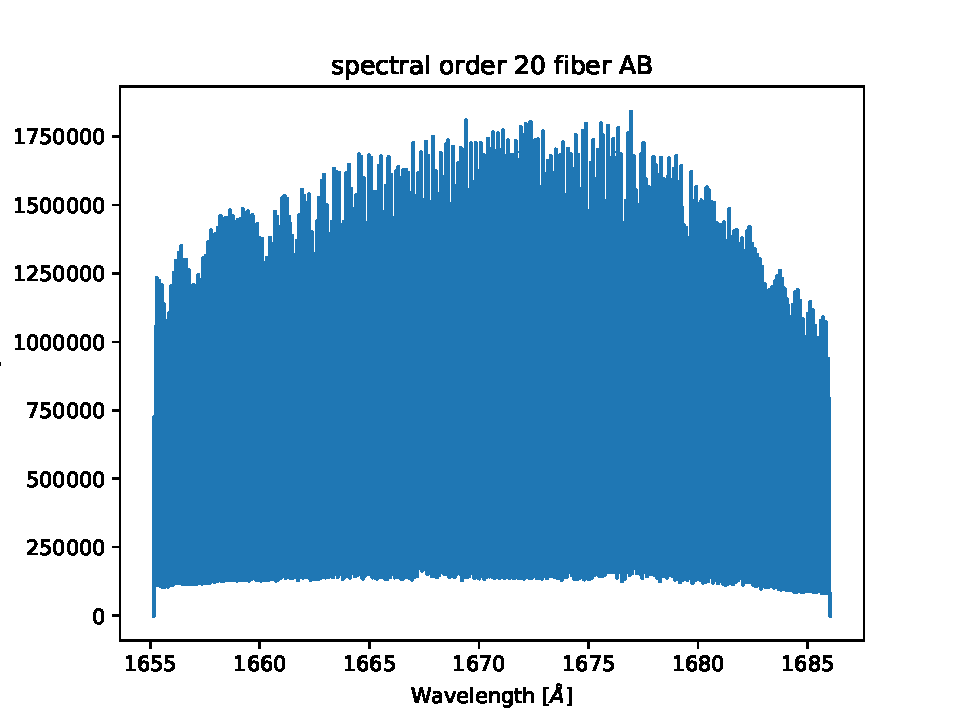
\includegraphics[width=\textwidth]{Figures/cal_ccf_e2ds_1.pdf}
a
\end{center}
\end{minipage}%
\begin{minipage}{.495\textwidth}
\begin{center}
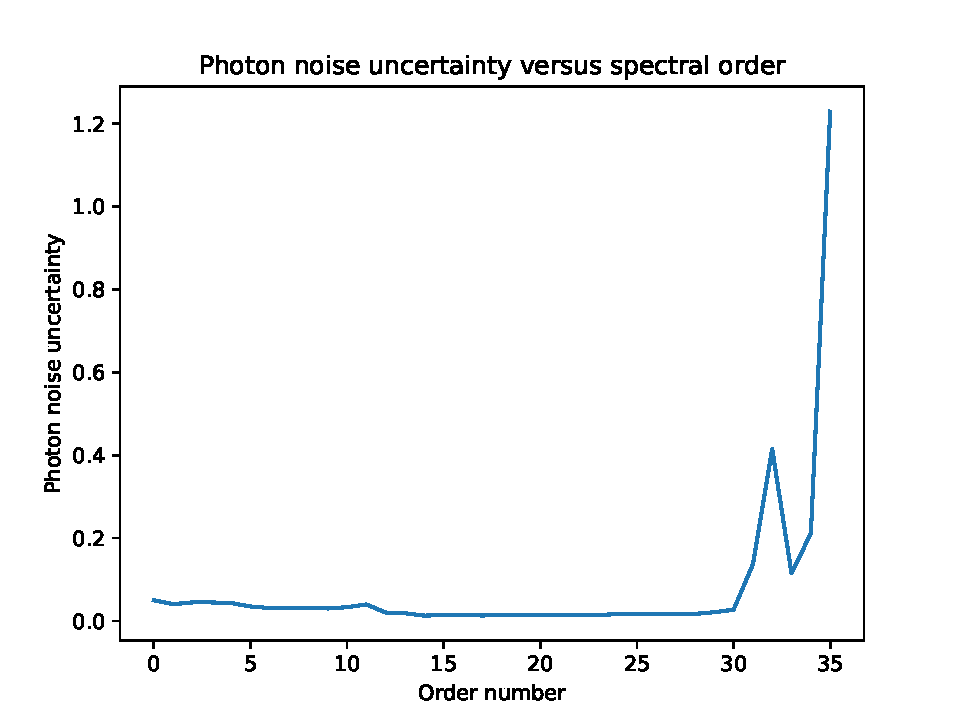
\includegraphics[width=\textwidth]{Figures/cal_ccf_e2ds_2.pdf}
b
\end{center}
\end{minipage}%
\end{center}

\begin{center}
\begin{minipage}{.495\textwidth}
\begin{center}
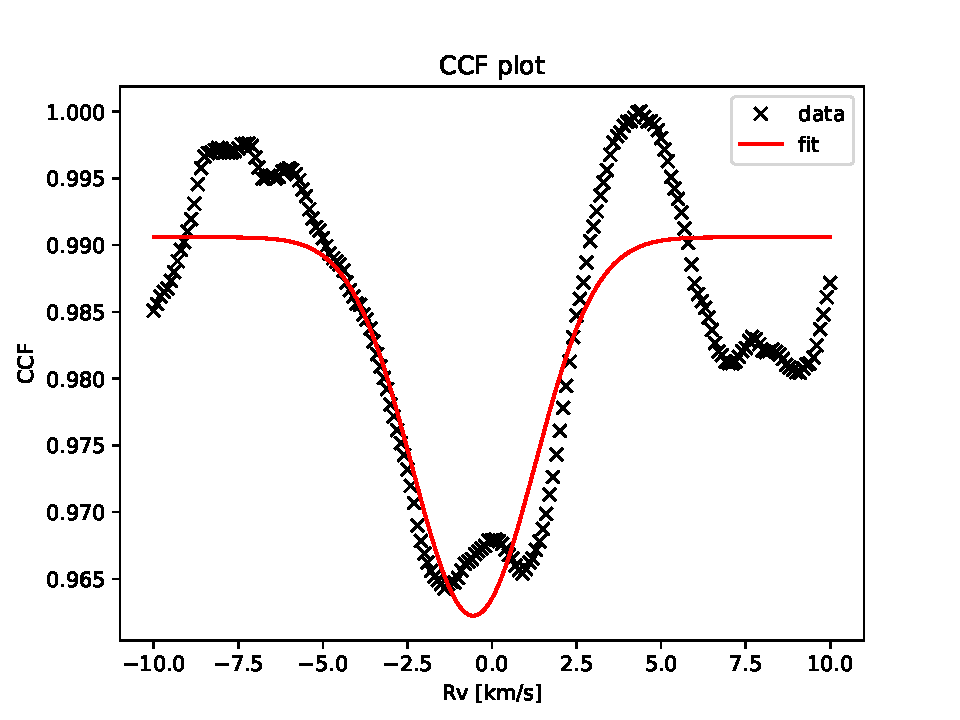
\includegraphics[width=\textwidth]{Figures/cal_ccf_e2ds_3.pdf}
c
\end{center}
\end{minipage}%
\end{center}

\caption{\textbf{(a)} The extract FP orders for spectral order 20, x-axis is wavelength and y-axis is extract flux. \textbf{(b)} Photon noise uncertainty versus spectral order. \textbf{(c)} The normalised CCF averaged across all orders, in red the fit to this CCF. \label{figure:cal_ccf_spirou}}
\end{figure}

%%%%%%%%%%%%%%%%%%%%%%%%%%%%%%%%%%%%%%%%%%%%%%%%%%%%%%%%
%%
\clearpage
\newpage
\section{The validation recipe}
\label{ch:the_recipes:cal_validate_spirou}
%%
%%%%%%%%%%%%%%%%%%%%%%%%%%%%%%%%%%%%%%%%%%%%%%%%%%%%%%%%

This recipe validates that the DRS has be installed correctly and insures that all recipes should run. This is mentioned in Section \ref{ch:install:validating_installunix}.
\begin{note}
The validation recipe does not protect against incorrect or missing constants and keywrods. If all constants are defined as they were when installed and if all paths were set up correctly, then running the validation recipe should be enough to confirm that the DRS installed correctly. Again this does not protect against invalid files and other user inputs.
\end{note}

% -------------------------------------------------------
\subsection{The inputs}
% -------------------------------------------------------
The \calvalidate recipe requires no input. Thus run the validation as follows:
\begin{cmdbox}
cal_validate_spirou.py
\end{cmdbox}
\noindent or
\begin{pythonbox}
import cal_validate_spirou
cal_validate_spirou.main()
\end{pythonbox}
\noindent One can also define an optional argument to put the validation recipe into debug mode with:
\begin{pythonbox}
import cal_validate_spirou
cal_validate_spirou.main(DEBUG=1)
\end{pythonbox}
\noindent where a value of True or 1 runs the validation script in debugging mode. This lists all sub-module tests that are performed during the validation and thus allows problems to be identified more easily.

% -------------------------------------------------------
\subsection{The outputs}
% -------------------------------------------------------

There are no outputs to \calvalidate other than printing to screen and the log file (see Section \ref{ch:the_recipes:cal_validate_spirou:example_run}).

% -------------------------------------------------------
\subsection{Summary of procedure}
% -------------------------------------------------------
\begin{enumerate}
\item checks core module imports:
	\begin{itemize}
	\item SpirouDRS
	\item \spirouConfig
	\item \spirouCore
	\end{itemize}
\item checks that configuration files can be read
\item checks recipe modules
	\begin{itemize}
	\item \spirouBACK
	\item \spirouCDB
	\item \spirouEXTOR
	\item \spirouFLAT
	\item \spirouImage
	\item \spirouLOCOR
	\item \spirouRV
	\item \spirouStartup
	\item \spirouTHORCA
	\end{itemize}
\item displays and prints the configuration file paths
\item confirms validation of the DRS installation
\end{enumerate}

% -------------------------------------------------------
\newpage
\subsection{Example working run}
\label{ch:the_recipes:cal_validate_spirou:example_run}
% -------------------------------------------------------

An example run where everything worked is below:

\begin{cmdbox}
cal_validate_spirou.py
\end{cmdbox}
\begin{cmdboxprintspecial}[fontupper=\tiny, fontlower=\tiny]
 *****************************************
 *        VALIDATING DRS 
 *****************************************

1) Running core module tests

2) Running config test

         Testing /drs/INTROOT/config/config.py

                Congraulations all paths in /drs/INTROOT/config/config.py set up correctly.

2) Running sub-module tests

4) Running recipe test

@gHH:MM:SS.S -   || *****************************************@g
@gHH:MM:SS.S -   || * SPIROU \@(#) Geneva Observatory (VERSION)@g
@gHH:MM:SS.S -   || *****************************************@g
@gHH:MM:SS.S -   ||(dir_data_raw)      DRS_DATA_RAW=/drs/data/raw@g
@gHH:MM:SS.S -   ||(dir_data_reduc)    DRS_DATA_REDUC=/drs/data/reduced@g
@gHH:MM:SS.S -   ||(dir_calib_db)      DRS_CALIB_DB=/drs/data/calibDB@g
@gHH:MM:SS.S -   ||(dir_data_msg)      DRS_DATA_MSG=/drs/data/msg@g
@gHH:MM:SS.S -   ||(print_level)       PRINT_LEVEL=all         %(error/warning/info/all)@g
@gHH:MM:SS.S -   ||(log_level)         LOG_LEVEL=all         %(error/warning/info/all)@g
@gHH:MM:SS.S -   ||(plot_graph)        DRS_PLOT=1            %(def/undef/trigger)@g
@gHH:MM:SS.S -   ||(used_date)         DRS_USED_DATE=undefined@g
@gHH:MM:SS.S -   ||(working_dir)       DRS_DATA_WORKING=/drs/data/tmp@g
@gHH:MM:SS.S -   ||                    DRS_INTERACTIVE is not set, running on-line mode@g
@gHH:MM:SS.S -   ||                    DRS_DEBUG is set, debug mode level:1@g
@gHH:MM:SS.S -   ||@g
@gHH:MM:SS.S -   ||Validation successful. DRS installed corrected.@g

\end{cmdboxprintspecial}



%%%%%%%%%%%%%%%%%%%%%%%%%%%%%%%%%%%%%%%%%%%%%%%%%%%%%%%%
%%
\clearpage
\newpage
\section{The cal\_HC recipe}
\label{ch:the_recipes:cal_HC_E2DS_spirou}
%%
%%%%%%%%%%%%%%%%%%%%%%%%%%%%%%%%%%%%%%%%%%%%%%%%%%%%%%%%

Recipe not yet updated.


%%%%%%%%%%%%%%%%%%%%%%%%%%%%%%%%%%%%%%%%%%%%%%%%%%%%%%%%
%%
\section{The cal\_WAVE recipe}
\label{ch:the_recipes:cal_WAVE_E2DS_spirou}
%%
%%%%%%%%%%%%%%%%%%%%%%%%%%%%%%%%%%%%%%%%%%%%%%%%%%%%%%%%

Recipe not yet updated.


%%%%%%%%%%%%%%%%%%%%%%%%%%%%%%%%%%%%%%%%%%%%%%%%%%%%%%%%
%%
\section{The pol\_spirou recipe}
\label{ch:the_recipes:pol_spirou}
%%
%%%%%%%%%%%%%%%%%%%%%%%%%%%%%%%%%%%%%%%%%%%%%%%%%%%%%%%%

Recipe not yet updated.


% Chapter: The Recipes
%%%%%%%%%%%%%%%%%%%%%%%%%%%%%%%%%%%%%%%%%%%%%%%%%%%%%%%%
%%
\chapter{The DRS Module}
\label{ch:the_module}
%%
%%%%%%%%%%%%%%%%%%%%%%%%%%%%%%%%%%%%%%%%%%%%%%%%%%%%%%%%


%%%%%%%%%%%%%%%%%%%%%%%%%%%%%%%%%%%%%%%%%%%%%%%%%%%%%%%%
%%
\section{The spirouBACK module}
\label{ch:the_module:spirouBACK}
%%
%%%%%%%%%%%%%%%%%%%%%%%%%%%%%%%%%%%%%%%%%%%%%%%%%%%%%%%%


%%%%%%%%%%%%%%%%%%%%%%%%%%%%%%%%%%%%%%%%%%%%%%%%%%%%%%%%
%%
\section{The spirouCDB module}
\label{ch:the_module:spirouCDB}
%%
%%%%%%%%%%%%%%%%%%%%%%%%%%%%%%%%%%%%%%%%%%%%%%%%%%%%%%%%


%%%%%%%%%%%%%%%%%%%%%%%%%%%%%%%%%%%%%%%%%%%%%%%%%%%%%%%%
%%
\section{The spirouCore module}
\label{ch:the_module:spirouCore}
%%
%%%%%%%%%%%%%%%%%%%%%%%%%%%%%%%%%%%%%%%%%%%%%%%%%%%%%%%%


%%%%%%%%%%%%%%%%%%%%%%%%%%%%%%%%%%%%%%%%%%%%%%%%%%%%%%%%
%%
\section{The spirouEXTOR module}
\label{ch:the_module:spirouEXTOR}
%%
%%%%%%%%%%%%%%%%%%%%%%%%%%%%%%%%%%%%%%%%%%%%%%%%%%%%%%%%


%%%%%%%%%%%%%%%%%%%%%%%%%%%%%%%%%%%%%%%%%%%%%%%%%%%%%%%%
%%
\section{The spirouFLAT module}
\label{ch:the_module:spirouFLAT}
%%
%%%%%%%%%%%%%%%%%%%%%%%%%%%%%%%%%%%%%%%%%%%%%%%%%%%%%%%%


%%%%%%%%%%%%%%%%%%%%%%%%%%%%%%%%%%%%%%%%%%%%%%%%%%%%%%%%
%%
\section{The spirouImage module}
\label{ch:the_module:spirouImage}
%%
%%%%%%%%%%%%%%%%%%%%%%%%%%%%%%%%%%%%%%%%%%%%%%%%%%%%%%%%


%%%%%%%%%%%%%%%%%%%%%%%%%%%%%%%%%%%%%%%%%%%%%%%%%%%%%%%%
%%
\section{The spirouLOCOR module}
\label{ch:the_module:spirouLOCOR}
%%
%%%%%%%%%%%%%%%%%%%%%%%%%%%%%%%%%%%%%%%%%%%%%%%%%%%%%%%%


%%%%%%%%%%%%%%%%%%%%%%%%%%%%%%%%%%%%%%%%%%%%%%%%%%%%%%%%
%%
\section{The spirouRV module}
\label{ch:the_module:spirouRV}
%%
%%%%%%%%%%%%%%%%%%%%%%%%%%%%%%%%%%%%%%%%%%%%%%%%%%%%%%%%


%%%%%%%%%%%%%%%%%%%%%%%%%%%%%%%%%%%%%%%%%%%%%%%%%%%%%%%%
%%
\section{The spirouStartup module}
\label{ch:the_module:spirouStartup}
%%
%%%%%%%%%%%%%%%%%%%%%%%%%%%%%%%%%%%%%%%%%%%%%%%%%%%%%%%%


%%%%%%%%%%%%%%%%%%%%%%%%%%%%%%%%%%%%%%%%%%%%%%%%%%%%%%%%
%%
\section{The spirouUnitTests module}
\label{ch:the_module:spirouUnitTests}
%%
%%%%%%%%%%%%%%%%%%%%%%%%%%%%%%%%%%%%%%%%%%%%%%%%%%%%%%%%



% % Appendi
% \appendix

% % \addtocontents{toc}{\setlength\cftchapternumwidth{1em}}

% % Appendix A: env_setup.sh
% \input{Chapters/appendix_env_setup_sh}

%%%---------------------------------------------------------

\backmatter

%%% BIBLIOGRAPHY
%%% -------------------------------------------------------------

% \bibliographystyle{utphysics}
% \bibliography{ref}

\end{document}
